% how to compile: platex xxx ; dvipdfmx xxx.dvi

%\documentclass[a4paper]{book}
\documentclass[a4paper]{jsbook}
\usepackage{mcmd_jp}
\usepackage{color}
\newcommand{\textColor}[3]{\colorbox{#1}{\color{#2}#3}}

\title{MCMD利用マニュアル}
\author{nysol corporation}
\date{}
\usepackage{makeidx}
\makeindex

\begin{document}
\begin{titlepage}
\begin{center}
{\huge MCMD利用マニュアル}\\
\vspace{10truept}
{\normalsize 対応NYSOLバージョン: Ver. 3.0}\\
\vspace{1cm}

履歴:\\
2017年4月30日 : Ver. 3.0対応\\
2016年6月30日 : 集計処理コマンドについての注意点追記、パラメータ微修正\\
2015年12月24日 : Ver. 2.4 対応、assert機能追加\\
2014年10月 6日 : Ver. 2.0 対応\\
2014年4月30日 : 例題のError修正など\\
2014年3月10日 : nysolパッケージへの統合に伴いインストール方法変更\\
2014年2月15日 : mxml2csv追加,微修正\\
2013年11月2日 : mpadding,mvnullto,mvdelnull追加,微修正\\
2013年9月20日 : 初期リリース\\
\vspace{13cm}
{\small \today}

{\small Copyright \copyright 2013-2017 by NYSOL CORPORATION}

\end{center}
\end{titlepage}

%\setlength{\baselineskip}{4mm}
\setcounter{tocdepth}{1}
\label{mcmd:toc}
\tableofcontents

\chapter{変更点}

%\begin{document}

\section{ver.2での変更点\label{sect:changes}}
\subsection{自動並べ替え機能の追加}

MCMD Ver. 1.0 では、たとえば\verb|msum|コマンドでキー項目を指定して集計する場合や、\verb|mjoin|コマンドで
複数のファイルをキー項目で結合する場合、事前に\verb|msortf|コマンドを使用してキー項目を並べ替えておく
必要があった。

多くのコマンドで事前の並べ替えが必要であり、また並べ替えを忘れてもエラーになることなく
誤った結果を出力して処理を終えるため、スクリプトにバグを生みやすいという難点があった。
そこで、\verb|k=|オプションでキー項目を指定するすべてのコマンドで、項目の並べ替えを自動的に行う
機能を追加したのがVer. 2.0の最大の変更点である。
どの項目で並べ替えられたのかがCSVヘッダの項目名にも追加されるため
(詳細は\hyperref[sect:csv_sort]{項目の並べ替え情報}参照)
、各コマンドは並べ替えが必要であるときのみ並べ替えを行う。

\subsubsection*{Ver. 1.0 での実行例}

\verb|msum k=顧客| コマンドを実行する前に、\verb|msortf|コマンドで\verb|顧客|項目を
並べ替えておく必要があった。

\begin{Verbatim}[baselinestretch=0.7,frame=single]
$ more dat1.csv
顧客,金額
A,10
B,10
A,20
B,15
B,20
$ msortf i=dat1.csv f=顧客 | msum k=顧客 f=金額:金額合計 o=rsl1.csv
#END# kgsortf f=顧客 i=dat1.csv
#END# kgsum f=金額:金額合計 k=顧客 o=rsl1.csv
$ more rsl1.csv
顧客,金額合計
A,30
B,45
\end{Verbatim}

\subsubsection*{Ver. 2.0 での実行例}

\verb|msum|コマンドが並べ替えの要否を判断し、必要であれば自身で並べ替えるため、
\verb|msortf|コマンドを省略しても正しい結果が得られる。
\verb|msum|コマンドが\verb|顧客|項目で並べ替えた証左として、
項目名に\verb|%0|が付加されている。


\begin{Verbatim}[baselinestretch=0.7,frame=single]
$ more dat1.csv
顧客,金額
A,10
B,10
A,20
B,15
B,20
$ msum i=dat1.csv k=顧客 f=金額:金額合計 o=rsl1.csv
#END# kgsum f=金額:金額合計 k=顧客 i=dat1.csv o=rsl1.csv
$ more rsl1.csv
顧客%0,金額合計
A,30
B,45
\end{Verbatim}
%\input{examples/tex/changes2_ex.tex}

\subsection{仕様が変更されたコマンド\label{sect:changedcommands}}

表\ref{tbl:changed_commands}に、Ver. 1.0 から仕様が変更されたコマンドを示す
(\verb|k=|パラメータに自動並べ替え機能が追加されたのみのコマンドを除く)。
行の順序が処理結果に影響するコマンドに\verb|s=|パラメータが追加されたほか、
いずれも行の並べ替えに関する仕様の変更である。

\begin{table}[!htbp]
\begin{center}
\caption{仕様が変更されたコマンド\label{tbl:changed_commands}}
{\small
  \begin{tabular}{l|l|l} \hline
コマンド                             & 説明               & 変更内容 \\ \hline
\hyperref[sect:maccum]{maccum}       & 累積計算           & \verb|s=|パラメータを追加(必須) \\
\hyperref[sect:mbest]{mbest}         & 指定行の選択       & \verb|s=|パラメータを追加(必須) \\
\hyperref[sect:mcombi]{mcombi}       & 組合せ計算         & \verb|s=|パラメータを追加 \\
\hyperref[sect:mkeybreak]{mkeybreak} & キーブレイク箇所   & \verb|s=|パラメータを追加 \\
\hyperref[sect:mmvavg]{mmvavg}       & 移動平均の算出     & \verb|s=|パラメータを追加(必須) \\
\hyperref[sect:mmvsim]{mmvsim}       & 移動窓の類似度計算 & \verb|s=|パラメータを追加(必須) \\
\hyperref[sect:mmvstats]{mmvstats}   & 移動窓の統計量の計算 & \verb|s=|パラメータを追加(必須) \\
\hyperref[sect:mnumber]{mnumber}     & 連番               & \verb|-B|使用時以外は\verb|s=|パラメータ必須に \\
\hyperref[sect:mpadding]{mpadding}   & 行補完コマンド     & \verb|type=|パラメータがなくなり、 \\
                                     &                    & 補完方法は\verb|f=|で指定するように \\
\hyperref[sect:mrjoin]{mrjoin}       & 参照ファイルの範囲条件による結合 & \verb|r=|パラメータで並べ替え方法を指定するように \\
\hyperref[sect:mslide]{mslide}       & 行ずらし           & \verb|s=|パラメータを追加(必須) \\
\hyperref[sect:mtra]{mtra}           & 縦型データをベクトル項目に変換 & \verb|s=|パラメータを追加 \\
\hyperref[sect:mwindow]{mwindow}     & スライド窓の生成   & \verb|wk=|パラメータで並べ替え方法を指定するように \\

\hline
  \end{tabular}
  }
  \end{center}
\end{table}

\subsection{従来のスクリプトを実行するには\label{sect:howtomodify}}

\verb|-q|オプションを使用すると、\verb|k=|パラメータで指定した項目の自動並べ替えが無効化される。
表\ref{tbl:changed_commands}で\verb|s=|パラメータが必須とされたコマンドで\verb|s=|パラメータを
省略できるようにもなるため、各コマンドはVer. 1.0と同等の動作をする。
よって、Ver. 1.0で使用していたスクリプトについては、\verb|k=|パラメータが指定された全コマンドに
\verb|-q|オプションを付加することでVer. 2.0でも同等の結果が得られる
(ただし\hyperref[sect:mpadding]{mpadding}コマンドについては、\verb|type=|パラメータが
なくなっているので、\verb|f=|パラメータでの指定に変更する必要がある)。

\subsubsection*{修正前のスクリプト}
Ver. 2.0環境で実行すると、\verb|maccum|コマンドに\verb|s=|パラメータがないというエラーが出る。
\begin{Verbatim}[baselinestretch=0.7,frame=single]
msortf i=customer.csv f=custID,date |
maccum k=custID f=amount o=accum.csv
#ERROR# parameter s= is mandatory without -q (kgaccum); kgaccum f=amount i=test.csv k=custID
\end{Verbatim}

\subsubsection*{修正例}
\verb|maccum|コマンドは\verb|s=|パラメータが必須となったが、
\verb|-q|オプションを追加することでVer. 1.0と同等の使い方ができる。
\begin{Verbatim}[baselinestretch=0.7,frame=single]
msortf i=customer.csv f=custID,date |
maccum -q k=custID f=amount o=accum.csv
\end{Verbatim}

\section{ver.3での変更点\label{sect:changes}}

MCMDをNYSOLパッケージから独立させGitHuBに登録したことにより、
バージョンを2.xから3.0へ上げた。
コマンド仕様の大きな変更はなく、以下に示す細かな点が改善されている。
また入力系コマンドを始めとして幾つかの新たなコマンドが追加されている。

\subsection{-paramsパラメータの追加}
全コマンド共通で-paramsパラメータを追加した。
主にシステム利用を目的としたもので、指定できるパラメータの一覧を標準出力に出力する。

\begin{Verbatim}[baselinestretch=0.7,frame=single]
$ mcut -params
-assert_diffSize
-assert_nullin
-nfn
-nfni
-nfno
-params
-r
-x
f=
i=
o=
precision=
tmpPath=
\end{Verbatim}

\subsection{環境変数KG\_msgTimebyfsec追加}
この環境変数をtrueに設定すると終了メッセージの時刻がマイクロ秒単位で表示される。

\begin{Verbatim}[baselinestretch=0.7,frame=single]
$ export KG_msgTimebyfsec=true
\end{Verbatim}

\subsection{mchkcsvの機能強化}

\begin{itemize}
 \item UTF BOMを自動的に除去する。
 \item -diagで内容が英語で出力され、-diaglで日本語で出力されるように変更。
\end{itemize}

\subsection{mcalの機能強化}
\begin{itemize}
 \item c=,a=に複数指定できるように変更。
 \item \verb|$t{},#t{},0t|でマイクロ秒までを扱えるように変更。
小数点(6桁)でマイクロ秒を表現している。
それに伴い、\verb|diffusecond(T,T),tuseconds(T),usecond(T),useconds(T),unow()|関数を追加。
 \item \verb|if(B,B,B)|のように、ブール値を返す使い方ができるようにする。
\end{itemize}

\subsection{mcatの機能強化}
\begin{itemize}
 \item \verb|-skip_zero|を指定することで、\verb|-nfn|を指定していない場合でも0バイトファイルでエラーにならない。
 \item \verb|flist=|を指定することで、併合するファイルリストをCSVデータとして指定することができるようにした。
        flist=fileName:fldNameで指定する。
 \item \verb|kv=|を指定することで、パス名に含めた"key-value"の文字列を抜き出し項目名とその値としてデータに付加する機能を追加。
\end{itemize}

\subsection{追加コマンド}
以下に示す画面入力系のコマンドが5つ追加された。
ただし、これらのコマンドは開発バージョンであり、今後仕様が変更される可能性がある。
\begin{itemize}
\item \hyperref[sect:minput] {minput} :入力画面を表示する。
\item \hyperref[sect:mminput] {mminput} : 複数入力枠による入力画面を表示する。
\item \hyperref[sect:mdsp] {mdsp} : 画面の指定位置に文字列を表示する。
\item \hyperref[sect:mseldsp] {mseldsp} : 画面に単一選択入力窓を表示する。
\item \hyperref[sect:mmseldsp] {mmseldsp} : 画面に複数選択入力窓を表示する。
\end{itemize}

その他にも以下に示すコマンドが追加された。
\begin{itemize}
\item \hyperref[sect:mshuffle] {mshuffle} :ハッシュキーによるファイル分割
\item \hyperref[sect:mcsvconv] {mcsvconv} : CSVを多様なフォーマットに変換
\item \hyperref[sect:mcsv2json] {mcsv2json} : CSVをjsonに変換
\end{itemize}

%\end{document}



\chapter{Mコマンド}
\index{えむこまんど@Mコマンド}

%\documentclass[a4paper]{book}
%\usepackage{zdd}
%\begin{document}

\section{Summary\label{sect:abstract}}
ZDD (Zero-suppressed Binary Decision Diagrams) is a data structure used for efficient manipulation of weighted item combinations based on reduction rules. ZDD VSOP (Valued-Sum-of-Products calculator)\cite{minato2005} is implemented as a Ruby Extension Library for the computation of item combinations. 

The founder of ZDD, Professor Shin-ichi Minato, developed a ZDD program which is made available for extended development in Ruby language. The Ruby Extension Library for ZDD is therefore developed in collaboration with \href{http://www-erato.ist.hokudai.ac.jp/index.php?language=jp}{ERATO Minato Discrete Structure Manipulation System Project}.

ZDD can enumerate huge number of combinations represented in a compact structure. For example, to enumerate all possible combinations of the products (frequent itemsets) purchased from the supermarket in the purchase history at a defined minimum support, in most cases, the number of combinations generated will grow exponentially. The ZDD data structure therefore is designed to provide a powerful framework to store all possible combinations in an unique and compact form efficiently.

Various calculations can be applied directly on ZDD objects where large scale itemsets are stored in a compact form for efficient processing.  
For example, users will be able to select the patterns containing "natto" from millions of enumerated frequent itemsets, or identify the differences of frequent itemset patterns between male and female. It is also possible to compute the ratio of size of ZDD. For details on theoretical context, please refer to \hyperref[sect:bib]{the reference} at the end of this document.

In this package, ZDD is handled as (known as {\bf ZDD object}) Ruby object.  Various functions for the ZDD objects correspond to class methods, operator overloading is used for ZDD objects using operands for ZDD object (\verb|+,-,==| etc.), to enable seamlessly integration of functions between Ruby and ZDD.

The ZDD package also supports automatic type conversion designed to reduce stress on   programming.

\section{Installation\label{sect:install}}
ZDD package is distributed as part of the mining package distribution by Nysol. Installation can be done by compiling from source or by installing rubygem.  Refer to mining package manual at \href{http://www.nysol.jp}{NYSOL} for details on the installation.

\section{Modify the maximum number of nodes}
The maximum number of ZDD nodes in this package is set to 40 million by default.
The program terminates with an error if the number of nodes exceeds this value.
The maximum number of nodes can be modified by setting the environment variable at \verb|ZDDLimitNode|.
For example, the maximum number of nodes can be set to 100 million nodes in the  bash shell as follows.
\begin{Verbatim}[baselinestretch=0.7,frame=single]
$ export ZDDLimitNode=100000000
\end{Verbatim}

The memory consumption per node is about 21-25 bytes on a 32bit OS machine. The program will consume about 1GB of main memory when the default limit of 40 million nodes is used. 

On a 64bit OS machine, the memory allocation is twice of the normal 32bit OS implementation, with 30\%percent increase in speed, and each node takes up to 28 to 32 bytes. Approximately 1.3GB of main memory is consumed when the program runs up to the default limit of 40 million nodes. By changing the maximum number of nodes according to the processing environment, the scale of ZDD structure can be increased.

\section{Terminologies\label{sect:terminology}}
The following section explains the terminologies used in this manual.
Note that there may be differences of the terms used in the \hyperref[sect:bib]{reference} at the end of this manual.

\subsubsection*{Item, Itemset, Term, Valued sum of products set, Expression}

An element in a set is referred to as "{\bf item}", and an "{\bf itemset}" contains a group of item elements.

The concept is easier to understand when these terms are set into context in a supermarket scenario. Commodity products are considered as items, and the combination of the products are referred to as itemset. When weight is attached to a "{\bf term}" in the itemset, it is known as "{\bf valued sum of products set}".
For example, the valued sum of products for 3 items a,b,c is represented as "\verb|abc+3ab+4bc+7c|" (this notation is referred to as "valued sum of products format"). It consists of four terms \verb|abc,3ab,4bc,7c|. In this case, \verb|3ab| consists of weight of \verb|3| for itemset \{a,b\}. Back to the supermarket scenario, this means that one customer purchased 3 products \verb|a,b,c| at the same time, and there are three customers who bought \verb|a,b| at the same time.

\subsubsection*{Empty itemset, ZDD constant object}
The itemset without element is referred to as "{\bf empty itemset}". Considering the valued sum of products set "\verb|abc+3ab+4bc+7c+3|", the a weight of \verb|3|  is attached to an empty itemset and thus it is shown as 3.

In supermarket scenario, it means that there are three customers did not purchase anything. 
Thus, empty itemsets of ZDD object is referred to as {\bf ZDD constant object}.

\subsubsection*{Item order table}
ZDD is a binary decision tree that contains a compact decision tree graph, and the level of the decision tree (depth) corresponds to the item. Further, this level, the order from  root to the leaves is managed by the table known as "{\bf item order table}".

It is important to manage item order since the order significantly impacts the size of ZDD (number of nodes). When the size of the ZDD increases, the processing speed will be reduced accordingly.
The item order table can be registered at any time using the \hyperref[sect:symbol]{symbol} function. If the number of combinations is extremely large, it is necessary to use the order table to register order of items.

\section{Notation\label{sect:notation}}

\subsubsection*{Notation of itemset}
The execution results in Ruby present the itemset which contains items and weight separated by space. Itemsets are displayed as character strings within text or comments, spaces between items are removed for simplicity.  For example, itemset \{a,b,c\} with weight of 3 is displayed as "\verb|3 a b c|" in the results. However, it will be displayed as "\verb|3abc|" in text or comment.

\subsubsection*{Example}

Multiple examples are included in this manual. The meaning of symbols used in the examples are as follows.\begin{itemize}
\item \verb|>| : Display Ruby input method.
\item \verb|$| : Display shell command line input.
\item \verb|#| : Display comments.
\item No symbol : Display the execution results.
\end{itemize}

The example contains the execution results log from the basic Ruby command line tool \verb|irb|. 


%\end{document}




%\begin{document}

\section{処理フロー(data processing flow)\label{sect:csv}}
nysol\_pythonでは、単一機能に特化した80以上のメソッドを自由に組み合わせることで、
データ処理の複雑なフローを構築することができ、その実行には最適な並列処理が適用される。
このようなフロー全体のことをデータ処理フローと呼ぶ。
そして処理フローを扱うパッケージがnysol.shellである。
以下では、単純な例から始め、nysol.shellがデータ処理フローをどのように扱うかについて説明する。

単純なデータ処理フローから始めよう。
図\ref{code:flow1}は、チュートリアルで示した図xを少し修正したフローである。
リストで表現された\verb|customer|と\verb|amount|の2項目3行のデータを読み込み、\verb|amount|項目のみを切り出し、
\verb|amount|項目を合計してリスト変数\verb|result|にセットするというものである。
チュートリアルとの違いは、全てのメソッドにソケット名を指定している点である。
nysolが提供するほとんどのメソッドには、他のメソッドとのデータのやりとりをするための口をもっており、それを{\bf ソケット}と呼ぶ。
ソケットには入力ソケットと出力ソケットがあり、それら入力と出力のソケットを接続することで処理フローを構成していく。

多くのメソッドにとって、パラメータ\verb|i=|と\verb|o=|は特殊な意味を持ち、
対象のメソッドに対する入力ソケット名、および出力ソケット名を指定するパラメータである。
ある処理Aの出力ソケット名と別の処理Bの入力ソケット名を同じにすることによりにより、
処理Aの出力データを処理Bの入力データに接続することができる。
図\ref{code:flow1}では、\verb|read|メソッドの出力ソケット(\verb|o=|)が\verb|mcut|メソッドの
入力ソケット(\verb|i=|)に\verb|p1|という名称にて接続されている。
ソケット名には任意の文字を用いることが可能であるが、\verb|_ns.|で始まる文字列はシステムによって予約されており利用できない。

データ処理フロー全体の接続関係を表示したければ、nysol.shellの\verb|topology|メソッドを用いれば良い(図\ref{code:flow1_topo}の1行目)。
\verb|name=|でhtmlファイル名を指定すれば図\ref{fig:flow1}のようなネットワーク図が出力される。
このネットワーク図には、ノードにメソッドが示され、エッジにソケットの接続関係が示される。
\verb|read|メソッドと\verb|mcut|メソッドを連結する有向エッジにラベル\verb|p1:o >> i|と示されているが、
これは、連結元の\verb|read|メソッドの出力ソケット\verb|o=|が\verb|mcut|メソッドの入力ソケット\verb|i=|に連結されていることを示している。
さらに、ノードにカーソルを合わせると、各メソッドに指定されたパラメータがポップアップで表示される。
ただしリストデータの内容は、省略表示される。

また\verb|topology|メソッドをパラメータなしで実行すれば、ネットワーク情報が辞書型データとして出力される。
図\ref{code:flow1_topo}に示されたネットワークの情報全てを含んでおり、
辞書のキーワードの意味を表\ref{tbl:flow_dic}に示す。


\begin{figure}[htbp]
\begin{Verbatim}[baselinestretch=0.7,frame=single]
>>> import nysol.mod as nm
>>> import nysol.flow as nf
>>> result=[]
>>> f=nf.new()
>>> f << nm.read(i=[["customer","amount"],["A",10],["B",50],["C",40]],o="p1")
>>> f << nm.mcut(f="amount",i="p1",o="p2")
>>> f << nm.msum(f="amount",i="p2",o="p3")
>>> f << nm.write(i="p3",o=result)
>>> f.run()
>>> print(result)
["amount"],[100]]
\end{Verbatim}
\caption{データ処理フローの例\label{code:flow1}}
\end{figure}

\begin{figure}[htbp]
\begin{Verbatim}[baselinestretch=0.7,frame=single]
>>> f.topology(name="flow1.html")
>>> g=f.topology()
>>> print(g["nodes"])
[0,1,2,3]
>>> print(g["methods"])
["read","mcut","msum","write"]
>>> print(g["params"])
[[("i",[]),("o","p1")],[("f","amount"),("i","p1"),("o","p2")],...]
>>> print(g["edges"])
[(0,1),(1,2),(2,3)]
>>> print(g["sockets"]
[("p1","o=","i="),("p2","o=","i="),("p3","o=","i=")]
\end{Verbatim}
\caption{データ処理フローのネットワーク情報を出力する\label{code:flow1_topo}}
\end{figure}

\begin{table}[hbt]
\begin{center}
 \caption{topologyメソッドで出力されるデータ処理フローのネットワークデータ\label{tbl:flow_dic}}
{\footnotesize
	\begin{tabular}{l|l|p{4cm}|p{8cm}}
\hline
キー & 内容 & 備考 & 図\ref{code:flow1_topo},\ref{fig:flow1}での例 \\
\hline
nodes   & ノードID   & 登録順に0から採番される。& \verb|[0,1,2,3]|: readメソッドのノードIDが0で、次のmcutメソッドのIDが1、以下同様。 \\
methods & メソッド名 & ノードIDに対応したメソッド名。& \verb|["read","mcut","msum","write"]|: ノードIDが0のメソッド名は\verb|read|で、IDが3のメソッド名は\verb|write|である。\\
params  & パラメータ & パラメータは(key,value)のタップルを要素に持ったリスト。& \verb|[[("i",[]),("o","p1")],...]|ノードIDが0のパラメータは\verb|i=[]|と\verb|o="p1"|である。ただし、データとして指定されたリストの内容は省略表記されることに注意する。\\
edgess  & エッジ     & 接続元ノードID(出力)と接続先ノードID(入力)のタップル & \verb|[(0,1),(1,2),(2,3)]|: ノードIDが0の\verb|read|の結合先はノードIDが1の\verb|mcut|である。\\
sockets & ソケット   & エッジに対応したソケットを、ソケット名、出力ソケット、入力ソケットのタップルで出力。 & \verb|[("p1","o=","i="),...]|: エッジ\verb|(0,1)|の接続ソケット名は\verb|p1|で、出力ソケットが\verb|o=|で、入力ソケットが\verb|i=|である。\\
\hline
 \end{tabular}
}
\end{center}
\end{table}

\verb|i=|であってもソケット名として解釈されないメソッドもある。
その一つが\verb|read|メソッドである。
\verb|read|メソッドの\verb|i=|に文字列を指定しても、それは入力ソケット名ではなくCSVファイル名として解釈される。
また同様に、\verb|write|メソッドの\verb|o=|に文字列を指定すれば、CSVファイル名として解釈される。

また、\verb|i=|と\verb|o=|以外にもソケットは存在し、
例えば\verb|mjoin|メソッドは入力ソケット\verb|i=|の他にもう一つ入力ソケット\verb|m=|を持っており、
結合対象となる参照データを指定することができる。
また、\verb|mselstr|メソッドは、出力ソケット\verb|o=|の他にもう一つ出力ソケット\verb|u=|を持っており、
条件にマッチしなかったデータの出力先を指定することができる。
このようにnysol.modでは、ソケット名を指定するパラメータはコマンドによって規定されている(表\ref{tbl:nysol.mod_socket})。

\begin{table}[hbt]
\begin{center}
 \caption{nysol.modが提供するメソッドのソケット指定パラメータ\label{tbl:nysol.mod_socket}}
{\footnotesize
	\begin{tabular}{l|p{10cm}|p{5cm}}
\hline
パラメータ & メソッド & 備考 \\
\hline
i=, o=    & m2tee$_*$, maccum, marff2csv, mavg, mbest, mbucket, mchgnum, mchgstr, mcombi, mcount, mcross, m2cross, mcsv2arff, mcut, mdformat, mduprec, mfldname, mfsort, mhashavg, mhashsum, mkeybreak, mmbucket, mmvavg, mmvsim, , , vstats, mnormalize, mnullto, mnumber, mpadding, mrand, msed, msetstr, mshare, msim, mslide, msortf, msplit, mstats, msum, msummary, mtab2csv, mtonull, mtra, mtrafld, mtraflg, muniq, mvcat, mvcount, mvdelim, mvdelnull, mvjoin, mvnullto, mvreplace, mvsort, mvuniq, mwindow, mxml2csv &
$_*$ m2teeは、o=に感まで区切って複数の出力ソケット名を記述できる。\\
i=, m=, o= & mcommon, mjoin, mnjoin, mnrcommon, mnrjoin, mpaste, mproduct, mrjoin, mvcommon &  \\
i=, u=, o= & mdelnull, mdata, msel, mselnum, mselrand, mselstr \\
o=       & mcat, mnewnumber, mnewrand, mnewstr \\
i=       & msep, msep2, mshuffle &
これら3つのメソッドは、\verb|o=|で実ファイルを指定しなければならない。
すなわち、次の接続のないメソッドである。\\
\hline
 \end{tabular}
}
\end{center}
\end{table}

図\ref{code:flow2}に、2つの入力ソケットを用いる例を示す。
この処理は図\ref{code:flow1}で計算した\verb|amount|の合計を元の3行データに結合(\verb|mproduct|)し、
各顧客の\verb|amount|の構成比を計算したものである。
ポイントは、\verb|read|メソッドの出力ソケット\verb|o=|が、2つのメソッド\verb|mcut,mproduct|に分岐して接続されており、
また、\verb|mproduct|メソッドが2つの入力ソケットにより接続されていることである。
データ処理フローのトポロジーの出力方法を図\ref{code:flow2_topo}に、その結果を\ref{fig:flow3}に示す。

\begin{figure}[htbp]
\begin{Verbatim}[baselinestretch=0.7,frame=single]
>>> import nysol.mod as nm
>>> import nysol.flow as nf
>>> result=[]
>>> f=nf.new()
>>> f << nm.read(i=[["customer","amount"],["A",10],["B",50],["C",40]],o="p1")
>>> f << nm.mcut(f="amount",i="p1",o="p2")
>>> f << nm.msum(f="amount:total",i="p2",o="p3")
>>> f << nm.mproduct(m="p3",f="total",i="p1",o="p4")
>>> f << nm.mcal(c="${amount}/${total}",a="share",i="p4",o="p5")
>>> f << nm.write(i="p5",o=result)
>>> f.run()
>>> print(result)
>>> [["customer","amount","total","share"],["A",10,100,0.1],["B",50,100,0.5],["C",40,100,0.4]]
\end{Verbatim}
\caption{フローが分岐する例\label{code:flow2}}
\end{figure}

\begin{figure}[htbp]
\begin{Verbatim}[baselinestretch=0.7,frame=single]
>>> f.topology(name="flow2.html")
>>> g=f.topology()
>>> print(g["nodes"])
[0,1,2,3,4,5]
>>> print(g["methods"])
["read","mcut","msum","mproduct","mcal","write"]
>>> print(g["params"])
[[("i",[]),("type","CSV"),("o","p1")],[("f","amount"),("i","p1"),("o","p2")],...]
>>> print(g["edges"])
[(0,1),(1,2),(2,3),(0,3),(3,4),(4,5)]
>>> print(g["sockets"]
[("p1","o=","i="),("p2","o=","i="),("p3","o=","i="),("p1","o=","i="),("p4","o=","i="),("p5","o=","i=")]
\end{Verbatim}
\caption{フローが分岐する場合のトポロジーの出力\label{code:flow2_topo}}
\end{figure}

\begin{figure}[htbp]
\begin{center}
\begin{tabular}{c}

\begin{minipage}{0.30\hsize}
\begin{center}
\includegraphics[scale=.25]{figure/flow/flow1.eps}
\end{center}
\caption{図\ref{code:flow1}のフロー図(flow1.html)\label{fig:flow1}}
\end{minipage}

\begin{minipage}{0.30\hsize}
\begin{center}
\includegraphics[scale=.25]{figure/flow/flow2.eps}
\end{center}
\caption{図\ref{code:flow2}のフロー図(flow2.html)\label{fig:flow1}}
\end{minipage}

\begin{minipage}{0.30\hsize}
\begin{center}
\includegraphics[scale=.25]{figure/flow/flow3.eps}
\end{center}
\caption{図\ref{code:flow2}の拡張フロー図(flow3.html)\label{fig:flow3}}
\end{minipage}

\end{tabular}
\end{center}
\end{figure}

このフローを実現させるために、nysol.shellは2つのメソッドを追加している。
まず、\verb|read|メソッドの出力を2つのフローに分岐させる\verb|mtee|メソッドを追加し、
\verb|mcut|へつながる流れと\verb|mproduct|へつながる流れを作る。

次に、バッファの機能を担う\verb|buffer|を挿入する。
nysol.shellでは、個々のメソッドはスレッドで実行され、2つのメソッドの接続にはパイプ(FIFOキュー)を用いている。
そしてデータの読み込みは基本的にはシーケンシャルreadによって実現している。
そのため、データ処理フローのトポロジーによってはデッドロックを起こす可能性がある。
例えば図\ref{code:flow2}の処理で、もし\verb|read|メソッドの入力データのサイズが非常に大きかった場合、
最終的に\verb|msum|が合計金額を計算するためには\verb|read|メソッドから全てのデータを読み切る必要がある。
一方で\verb|mproduct|メソッドは、その\verb|total|が\verb|m=|ソケットを通して届かない限り、
\verb|read|メソッドからのデータを読み込みできない状態が続く。
パイプのバッファサイズは通常さほど大きくはないのでデッドロックを起こしてしまう。
そのため、\verb|nysol.sell|では、そのようなデッドロックが起こる可能性のある箇所に巨大バッファをメソッドとして挿入する。

最終的に\verb|nysol.shell|が追加修正したフロー図({\bf 拡張フロー図}と呼ぶ)を表示したければ、
図\ref{code:flow3}にあるように、\verb|topology|メソッドに\verb|extention=True|を指定すればよい。
すると図\ref{fig:flow3}のように、nysol.shellによって\verb|buffer|メソッドが追加されたフローを確認できるであろう。

\begin{figure}[htbp]
\begin{Verbatim}[baselinestretch=0.7,frame=single]
>>> f.topology(name="flow3.html",extention=True)
\end{Verbatim}
\caption{拡張フロー図の表示例\label{code:flow3}}
\end{figure}

\subsection{ソケット名の省略}
前節では、説明のために全てのメソッドに入出力ソケット名を指定したが、
多くの場合、ソケット名は省略することが可能である。

2つの連続するメソッドをA,Bとすると、

A,B共にAにo=がなく、Bにi=がない: A(o=\_ns.num)
Aの

よって、図\ref{code:flow1}のフローは図\ref{code:flow1_omit}のように全てのソケット名を省略することができる。
一方で図\ref{code:flow2}のフローは、\verb|mproduct|の入力ソケット\verb|p1|が3行前の\verb|read|であるため省略できない。
m=を省略できる

\begin{figure}[htbp]
\begin{Verbatim}[baselinestretch=0.7,frame=single]
>>> import nysol.mod as nm
>>> import nysol.flow as nf
>>> result=[]
>>> f=nf.new()
>>> f << nm.read(i=[["customer","amount"],["A",10],["B",50],["C",40]],o="p1")
>>> f << nm.mcut(f="amount",i="p1",o="p2")
>>> f << nm.msum(f="amount:total",i="p2",o="p3")
>>> f << nm.mproduct(m="p3",f="total",i="p1",o="p4")
>>> f << nm.mcal(c="${amount}/${total}",a="share",i="p4")
>>> f << nm.write(o=result)
>>> f.run()
>>> print(result)
>>> [["customer","amount","total","share"],["A",10,100,0.1],["B",50,100,0.5],["C",40,100,0.4]]
\end{Verbatim}
\caption{フローが分岐する例\label{code:flow2}}
\end{figure}

\subsection{I/Oメソッド}
処理フローの中では、データはCSV形式のバイトストリームとして流れていく。
一方で、処理対象とするデータとしては、例えばCSVファイルや、
pythonのリスト、pandasパッケージのデータフレームなど多様なタイプのデータがあるであろう。
nysol.shellにとって\verb|read|と\verb|write|メソッドは、それらの様々なデータタイプとデータストリームを相互に変換する機能を担っている。
\verb|read,write|メソッドが扱えるデータタイプは以下のとおりで、いずれも固定数の列と可変数の行を備えたデータある。
特定のデータタイプの選択は\verb|type=|パラメータで指定する。
最後の項目のパラメータについては、他のデータタイプとは異なり、データを指定せずに後に\verb|run|メソッドの中で指定する方式で、
これは処理フローを新たなメソッドとして登録する方法であり、後の節で詳述する。

\begin{table}[hbt]
\begin{center}
 \caption{read,writeメソッドが扱うことのできるデータタイプ一覧\label{tbl:nysol.mod_socket}}
{\footnotesize
	\begin{tabular}{l|l|l}
\hline
データタイプ名 & \verb|type=|で指定する値 & 説明 \\
\hline
CSVファイル & \verb|"csv"|    & 複数の同一構造のCSVファイル \\
ディレクトリ& \verb|"dir"|    & 複数のCSVファイルを含んだディレクトリ階層 \\
リストデータ& \verb|"list"|   & pythonのリスト型データ \\
辞書型データ& \verb|"dic"|    & pythonの辞書型データ \\
pandasデータ& \verb|"pandas"| & pandasパッケージが扱うデータフレーム \\
numpyデータ & \verb|"numpy"|  & numpyパッケージが扱う2階テンソル \\
パラメータ  & \verb|"param"|  & ユーザが\verb|run|メソッドでデータを与える \\
\hline
 \end{tabular}
}
\end{center}
\end{table}

\subsubsection*{CSVファイル}
同一の項目名を備えた複数のCSVファイルを指定できる。
図\ref{code:io_csv1}は、単一のCSVファイル\verb|input.csv|を読み込み、\verb|mcut|メソッドで全項目を選択し、
CSVファイル\verb|output.csv|に書き込む例である。
\verb|output.csv|の内容は\verb|input.csv|の内容と同じになる。

\begin{figure}[htbp]
\begin{Verbatim}[baselinestretch=0.7,frame=single]
>>> # input.csvの内容(pythonを実行したディレクトリに存在するものとする)
>>> # a,b,c
>>> # x,1,0.1
>>> # y,2,0.2
>>> f=nf.new()
>>> f << nm.read(i="input.csv",type="csv")
>>> f << nm.mcut(f="a,b,c")
>>> f << nm.write(o="output.csv",type="csv")
>>> f.run()
\end{Verbatim}
\caption{CSVファイルの読み込みと書き込み(nm,nsのimport文は省略している)\label{code:io_csv1}}
\end{figure}

複数のファイルを行方向に併合して読み込むには、複数のCSVファイル名をリストに格納して\verb|i=|に指定してやれば良い
(一つのファイル名を指定した先程の例でもリストにファイル名を一つ格納して与えてもよい)。
図\ref{code:io_csv2}では、2つのファイルを併合して、先程の例と同様にそのままCSVファイルとして出力している。
入力ファイルが多数ある場合は、\verb|glob|パッケージ等を用いて事前にファイル名一覧をリストにセットしておけばよい(図\ref{code:io_csv3})。
複数のCSVファイルを指定する場合に項目名が異なる場合は、
リストの最初に指定したCSVの項目が採用され、それ以降のCSVデータに項目がなければNULL値が出力され、
また余分な項目は無視される。
ただし、\verb|name=|パラメータに必要な項目名を指定すれば、それらの項目名が併合対象として優先される。
なお、ファイル名にワイルドカードを使って複数ファイルを指定することはできない。

\begin{figure}[htbp]
\begin{Verbatim}[baselinestretch=0.7,frame=single]
>>> # input1.csv,input2.csvの内容は以下の通り同じものとする。
>>> # a,b,c
>>> # x,1,0.1
>>> # y,2,0.2
>>> f=nf.new()
>>> f << nm.read(i=["input1.csv","input2.csv"],type="csv")
>>> f << nm.mcut(f="a,b,c")
>>> f << nm.write(o="output.csv",type="csv")
>>> # output.csvの内容は以下の通り。
>>> # a,b,c
>>> # x,1,0.1
>>> # y,2,0.2
>>> # x,1,0.1
>>> # y,2,0.2
>>> f.run()
\end{Verbatim}
\caption{複数のCSVファイルの読み込みと書き込み\label{code:io_csv2}}
\end{figure}

\begin{figure}[htbp]
\begin{Verbatim}[baselinestretch=0.7,frame=single]
>>> import glob
>>> f=nf.new()
>>> f << nm.read(i=glob.glob("input*.csv"),type="csv")
>>> f << nm.mcut(f="a,b,c")
>>> f << nm.write(o="output.csv",type="csv")
>>> f.run()
\end{Verbatim}
\caption{図\ref{code:io_csv2}の例をワイルドカードを使って実行する例\label{code:io_csv3}}
\end{figure}


\subsubsection*{ディレクトリ}
ディレクトリ名を指定すれば、そのディレクトリ内にある全てのCSVファイルを併合してデータストリームに変換する。
ディレクトリは階層になっていてもよく、指定したディレクトリの下に存在する全てのCSVデータが対象となる。
これらのCSVデータの併合順序は不定である。
図\ref{code:io_dir}では、\verb|inputs|ディレクトリにある2つのファイルを併合して読み込む例である。
\begin{figure}[htbp]
\begin{Verbatim}[baselinestretch=0.7,frame=single]
>>> # 以下の同じ内容を持つinput1.csv,input2.csvがinputsディレクトリに存在するとする。
>>> # a,b,c
>>> # x,1,0.1
>>> # y,2,0.2
>>> f=nf.new()
>>> f << nm.read(i="inputs",type="dir",name="a,b,c")
>>> f << nm.mcut(f="a,b,c")
>>> f << nm.write(o="output.csv",type="csv")
>>> f.run()
>>> # output.csvの内容は以下の通り。
>>> # a,b,c
>>> # x,1,0.1
>>> # y,2,0.2
>>> # x,1,0.1
>>> # y,2,0.2
\end{Verbatim}
\caption{ディレクトリ名を指定して実行する例\label{code:io_dir}}
\end{figure}

\subsubsection{リストデータ}
\subsubsection{辞書型データ}
\subsubsection{pandasデータ}
\subsubsection{numpyデータ}

\subsection{パラメータ}

\subsection{処理フローのネットワークに島ができる場合}
島(連結成分)ができるということは、処理順序に依存関係がないということである。

登録順に実行される。
独立した処理フローをわざわざ一つのフローの中に入れて実行するメリットは並列処理にある。
nysol.shellでは、処理フローの中に島になったフローが複数あれば、それらを並列で実行する。

\begin{figure}[htbp]
\begin{Verbatim}[baselinestretch=0.7,frame=single]
>>> import nysol.mod as nm
>>> import nysol.flow as nf
>>> results={}
>>> f=nf.new()
>>> for tax_rate in [0.05,0.08,0.1]:
>>>   results[tax_rate]=[]
>>>   f << nm.read(i=[["amount"],[100]])
>>>   f << nm.mcal(c="${amount}*%g"%(tax_rate), a="tax")
>>>   f << nm.write(o=results[tax_rate])
>>> f.run()
>>> print(results)
{0.05:[["amount","tax"],["100","5"]] ,0.08:[["amount","tax"],["100","8"]] , 0.1:[["amount","tax"],["100","10"]]}
\end{Verbatim}
\caption{独立の処理フローを並列処理する例\label{code:flow_para1}}
\end{figure}

図\ref{code:flow_para2}は、図\ref{code:flow_para1}の処理を逐次実行するように変更したものである。
変更点は一箇所、\verb|f.run()|を\verb|for|文の中に入れた点である。

\begin{figure}[htbp]
\begin{Verbatim}[baselinestretch=0.7,frame=single]
>>> import nysol.mod as nm
>>> import nysol.flow as nf
>>> results={}
>>> f=nf.new()
>>> for tax_rate in [0.05,0.08,0.1]:
>>> 	results[tax_rate]=[]
>>>   f << nm.read(i=[["amount"],[100]])
>>>   f << nm.mcal(c="${amount}*%g"%(tax_rate), a="tax")
>>>   f << nm.write(o=results[tax_rate])
>>>   f.run()
>>> print(results)
{0.05:[["amount","tax"],["100","5"]] ,0.08:[["amount","tax"],["100","8"]] , 0.1:[["amount","tax"],["100","10"]]}
\end{Verbatim}
\caption{独立の処理フローを逐次処理する例\label{code:flow_para2}}
\end{figure}

\subsubsection{制限}
処理フローは時に非常に大きくなる可能性がある。
店別のデータがあって、全ての店に同じ処理を実行したい場合、
一つの処理フローの中に店の数だけ独立したフローができることになる。
10万店あるチェーン店であった場合、それらを並列処理して大丈夫であろうか?

pipeで2
ソートが走ると32
macの場合の制限10240


%\end{document}


%
%\begin{document}

\section{CSV\label{sect:csv}}
MCMD processes spreadsheet data in CSV format (Comma Separated Values) as illustrated in Figure \ref{fig:csv_exp1}. CSV is a \textit{de facto} standard format for spreadsheet data. It is widely used as an intermediate format for data interchange between different application programs.

\begin{figure}[hbt]
\begin{Verbatim}[baselinestretch=0.7,frame=single]
Product code, product name, classification, price
0899781,bread, food,128
8879674,orange juice, beverage,98 3244565,cheese, food,350
6711298,bowl, tableware,168
\end{Verbatim}
\caption{Example of CSV data\label{fig:csv_exp1}}
\end{figure}

\begin{figure}[hbt]
\begin{Verbatim}[baselinestretch=0.7,frame=single]
(A) file = [header CRLF] record *(CRLF record) [CRLF]
(B) header = name *(COMMA name)
(C) record = field *(COMMA field)
(D) name = field
(E) field = (escaped / non-escaped)
(F) escaped = DQUOTE *(TEXTDATA / COMMA / CR / LF / 2DQUOTE) DQUOTE
(G) non-escaped = *TEXTDATA
(H) COMMA = %x2C
(I) CR = %x0D ;as per section 6.1 of RFC 2234 [2]
(J) DQUOTE = %x22 ;as per section 6.1 of RFC 2234 [2]
(K) LF = %x0A ;as per section 6.1 of RFC 2234 [2]
(L) CRLF = CR LF ;as per section 6.1 of RFC 2234 [2]
(M) TEXTDATA = %x20-21 / %x23-2B / %x2D-7E
\end{Verbatim}

\caption{Definition of ABNF for CSV\label{fig:csv_abnf}}
\end{figure}

The meaning of each line in Figure \ref{fig:csv_abnf} is as follows:

\begin{itemize}
\item (A) File consists of a header and record of one or more lines. A header is not required. The line break (CRLF) is attached at the end of the header and at each record. The line break (CRLF) in the last row is not required.
\item (B) Header consists of one or more names separated by a single comma.
\item (C) Record consists of one or more fields separated by a single comma.
\item (D) Name refers to field.
\item (E) Field can include an escape character or a non-escape character.
\item (F) Field values containing 1 or more text characters (TEXTDATA), comma(COMMA), and a newline character (CR or LF) shall have a pair of consecutive double quotes character escaped by doubling it.
\item (G) Non-escape refers to 1 or more text characters (TEXTDATA).
\item (H) ASCII code of comma in hexadecimal is 2C.
\item (I) ASCII code of carriage return (CR) in hexadecimal is 0D.
\item (J) ASCII code of double quotation (DQUOTE) in hexadecimal is 22.
\item (K) ASCII code of line feed (LF) in hexadecimal is 0A.
\item (L) Line break or newline is represented as a carriage return + line feed.
\item (M) Text character (TEXTDATA) had the range of 20-21, 23-2B, 2D-7E in hexadecimal ASCII code.
\end{itemize}

\subsection{Definition specific to MCMD}
In addition to the above definitions, MCMD has the following restrictions regarding CSV:

\begin{itemize}
\item The number of fields must be the same in all the rows.
\item There is a limit on the maximum length of a single row (1024000 bytes (1 MB) by default and expandable to 10 MB by changing the value of \verb|KG_LimitRecLen| in the source code kgConfig.h).
\item Line break is only marked with Line Feed (LF).
\item Line break is mandatory even in the last record.
\item Added the 80-FF (hexadecimal) range to text characters for handling multibyte characters.
\end{itemize}
To check if a CSV file meets the above definitions, use the \hyperref[sect:mchkcsv]{mchkcsv} command.

\subsection{Common input and output process}
The input and output sequence of CSV file for MCMD follows the steps listed below.

\begin{enumerate}
\item Read file into memory blocks.
\item Split the comma-delimited string into different fields while taking consideration of escape character.
\item Interpret escape characters and convert to original data (except DQUOTE).
\item Run the specific processing function of the command and write the results to the output buffer.
\item Add character escapes if necessary.
\item Output to a file when buffer is full.
\end{enumerate}


\subsection{Field sorting information\label{sect:csv_sort}}
When the msortf command is used to sort fields or the \verb|s=| or \verb|k=| parameter is used in any other command, records in the specified fields will be sorted. Then, sorting information is added to the fieldnames in the output CSV file. Specifically, numerals will be added to the fieldnames in the order they are specified as sorting fields, starting with a zero: \verb|%0|, \verb|%1|, and so on. When the fields are sorted as numerical values, \verb|n| will be added. When they are sorted in the descending order, \verb|r| will be added. The added information is internally used by the commands for efficiency; the user must not specify it as part of a fieldname.

\begin{Verbatim}[baselinestretch=0.7,frame=single]
$ cat dat1.csv
id,item,price
2,b2,200
1,a1,100
2,b1,120
$ msortf f=id,price%n i=dat1.csv
id%0,item,price%1n
1,a1,100
2,b1,120
2,b2,200
$ msum k=id f=price i=dat1.csv
id%0,item,price
1,a1,100
2,b1,320
\end{Verbatim}

To delete the added information, run \verb|mfldname -q| as described below.

\begin{Verbatim}[baselinestretch=0.7,frame=single]
$ cat dat2.csv
id%0,item,price%1n
1,a1,100
2,b1,120
2,b2,200
$ mfldname i=dat2.csv
id,item,price
1,a1,100
2,b1,120
2,b2,200
\end{Verbatim}

If the fieldname sorting information does not match the actual sequence of records (for instance, a fieldname includes \verb|%0| although records have not been sorted), the operation of the commands is indefinite.

\subsection{Notes}
Points to note when preparing the CSV data will be described below with examples.

\subsubsection{Data containing comma characters}
Escape comma characters in data by enclosing them in double quotes.
The following is a CSV file comprising of two fields \verb|f1,f2|. 
The data in row 01 at column \verb|f1| is enclosed in double quotes since it contains a comma.

\begin{Verbatim}[baselinestretch=0.7,frame=single]
f1,f2
"abc,def",2
xyz,2
\end{Verbatim}
\footnote{MCMD address the value of the first row as 0 (except for the field name row) consistently.}

\subsubsection{Data containing double quotes}
Data containing double quotes characters can be represented by a pair of consecutive double quotes. The following is the CSV file that consists of two columns \verb|f1,f2|. Data in row 0 and 1 at column \verb|f1| is escaped with a double quotation. The original data is written as \verb|abc"def| and \verb|"| respectively.

\begin{Verbatim}[baselinestretch=0.7,frame=single]
f1,f2
"abc""def",2
"""",2
\end{Verbatim}

\subsubsection{Line breaks in data}
Data including a line break can be a process when enclosed in double quotes. A line break is included in the data at row 0 in column \verb|f1| after \verb|abc|. Since the data is enclosed in double quotes, it is identified as part of the data instead of the end of the line.

\begin{Verbatim}[baselinestretch=0.7,frame=single]
f1,f2
"abc
def",1
\end{Verbatim}

\subsubsection{Unnecessary double quotes}
Unnecessary double quotes are removed in the output.

\begin{Verbatim}[baselinestretch=0.7,frame=single]
$ more data.csv
f1,f2
"abc",efg
abc,"efg"
$ mcut f=f1,f2 i=data.csv
f1,f2
abc,efg
abc,efg
\end{Verbatim}

%\end{document}


%
%\begin{document}

\section{データ型\label{sect:datatype}}
MCMDで扱うCSVデータはプレーンテキストであり、全てのデータは文字列で表されている。
よってその文字列をどのようなデータ型として扱うかはコマンドによって決まる。
例えば、\verb|msum|コマンドで\verb|f=|で指定した項目データは、コマンド内部で文字列から数値へと変換される。
MCMDで扱うことのできる型は、表\ref{tbl:datatype_types}に示される通り、
数値型、文字列型、日付型、時刻型、論理型、ベクトル型の6つである。

\begin{table}[!hb]
\begin{center}
\caption{MCMDが扱う6つのデータ型\label{tbl:datatype_types}}
{\small
  \begin{tabular}{l|l|l} \hline
データ型  & CSVデータ表記例        & 変換内容 \\ \hline
数値型    & 10, 2.5, 1.5E+10       & 倍精度実数 \\
文字列型  & abc, あいう            & 文字列 \\
日付型    & 20130920               & 日付オブジェクト$^{*1}$(グレゴリオ暦,8桁固定長) \\
時刻型    & 20130920151154.123456  & 日付オブジェクト$^{*1}$(グレゴリオ暦,8桁固定長) \\
          &                        & \ \ \ \ +POSIX時刻$^{*2}$(6桁の時分秒+最大小数6桁のマイクロ秒) \\
          & 151154.123456          & 日付が指定されていない場合は、内部的には本日日付が付加される \\
論理型    & 1,0                    & "1"を真、"0"を偽のbool値に変換する \\
ベクトル型& a c b, 1 5 11          & スペースで区切られた文字列を、上記のいずれかのデータ型に変換したもの \\
\hline
  \end{tabular}
\\
$^{*1}$ boostライブラリのboost::gregorian::dateクラスを利用 \\
$^{*2}$ boostライブラリのboost::posix\_time::ptimeクラスを利用 \\
  }
  \end{center}
\end{table}

また、表\ref{tbl:datatype_commands}に各データ型として扱う代表的なコマンドを示しておく。

\begin{table}[!hb]
\begin{center}
\caption{各データ型を扱う代表的なコマンド\label{tbl:datatype_commands}}
{\small
  \begin{tabular}{l|l|l} \hline
データ型  & コマンド               & 内容 \\ \hline
数値型    & \hyperref[sect:msum]{msum} & 数値項目の合計計算 \\
          & \hyperref[sect:msim]{msim} & 2つの項目の類似度計算 \\
\hline
文字列型  & \hyperref[sect:mjoin]{mjoin} & 参照ファイルの項目の結合 \\
          & \hyperref[sect:mcombi]{mcombi} & 組み合せの列挙 \\
\hline
日付型    & \hyperref[sect:mcal]{mcal}の\hyperref[sect:age]{age}関数 & 年齢計算 \\
          & \hyperref[sect:mcal]{mcal}の\hyperref[sect:leapyear]{leapyear}関数 & 閏年の判定 \\
\hline
時刻型    & \hyperref[sect:mcal]{mcal}の\hyperref[sect:now]{now}関数 & 現在時刻の出力(秒単位) \\
          & \hyperref[sect:mcal]{mcal}の\hyperref[sect:unow]{unow}関数 & 現在時刻の出力(マイクロ秒単位) \\
          & \hyperref[sect:mcal]{mcal}の\hyperref[sect:diff]{diffminute}関数 & 分単位での時刻差の計算 \\
\hline
論理型    & \hyperref[sect:mcal]{mcal}の\hyperref[sect:and]{and}関数 & 論理積の計算 \\
          & \hyperref[sect:mcal]{mcal}の\hyperref[sect:if]{if}関数  & 条件による値の設定 \\
\hline
ベクトル型& \hyperref[sect:mvsort]{mvsort}    & ベクトル要素の並べ替え \\
          & \hyperref[sect:mvuniq]{mvuniq}    & ベクトル要素の単一化 \\
\hline
  \end{tabular}
  }
  \end{center}
\end{table}


%
%\begin{document}

\section{項目の指定\label{sect:fieldname}}
MCMDでは、CSVデータの先頭行を項目名として扱うことも可能であるし、
また項目名行がなくても項目番号で項目を指定することもできる。
項目名行の扱いに関係するパラメータは-nfn,-nfno,-nfni,-xの4つある。
以下では、例を示しながら、その利用方法について説明する。
なお、項目番号は左から0,1,2のように0から始まることに注意する。

\subsubsection*{例1: -nfn指定}

\verb|-nfn|(no field names)を指定すると,先頭行を項目名行と見なさない。
そして項目は必ず番号で指定する(番号は0から始まることに注意する)。


\begin{Verbatim}[baselinestretch=0.7,frame=single]
$ more dat2.csv
a,2
b,5
b,4
$ msum -nfn k=0 f=1 i=dat2.csv o=rsl1.csv
#END# kgsum -nfn f=1 i=dat2.csv k=0 o=rsl1.csv
$ more rsl1.csv
a,2
b,9
\end{Verbatim}
\subsubsection*{例2: -nfno指定}

\verb|-nfno|(no field names for output)を指定すると,入力データの先頭行は項目名行として扱うが,出力データには項目名を出力しない.


\begin{Verbatim}[baselinestretch=0.7,frame=single]
$ more dat1.csv
key,val
a,2
b,5
b,4
$ msum k=key f=val -nfno i=dat1.csv o=rsl2.csv
#END# kgsum -nfno f=val i=dat1.csv k=key o=rsl2.csv
$ more rsl2.csv
a,2
b,9
\end{Verbatim}
\subsubsection*{例3: -nfni指定}

\verb|-nfni|(no field name for input)の指定はmcutでのみ可能であるオプションである.
このオプションは-nfnoと逆の働きをする.
すなわち,入力データの先頭行は項目名行として扱わないが,
出力データには項目名を出力する.
よって、入力項目番号に続けて出力項目名を":"に続けて指定する必要がある.


\begin{Verbatim}[baselinestretch=0.7,frame=single]
$ mcut f=0:key,1:val -nfni i=dat2.csv o=rsl3.csv
#END# kgcut -nfni f=0:key,1:val i=dat2.csv o=rsl3.csv
$ more rsl3.csv
key,val
a,2
b,5
b,4
\end{Verbatim}
\subsubsection*{例4: -x指定}

項目名行があるCSVデータに対して、項目番号で指定したい場合は\verb|-x|オプションを利用する。


\begin{Verbatim}[baselinestretch=0.7,frame=single]
$ msum -x k=0 f=1 i=dat1.csv o=rsl4.csv
#END# kgsum -x f=1 i=dat1.csv k=0 o=rsl4.csv
$ more rsl4.csv
key%0,val
a,2
b,9
\end{Verbatim}


\subsection{有効な項目名}

項目名として利用可能な文字は以下の通りである。
\begin{itemize}
\item アルファベット(a-z,A-Z)
\item 数字(0-9)
\item マルチバイト文字(UTF-8など)
\item 記号
\end{itemize}

ただし、記号については、以下の9つの利用は避けることを推奨する。
利用してエラーとなるわけではないが、いずれもMCMDの中で項目指定時の特殊文字として利用しており
その特殊用途を利用できなくなる可能性があるからである。

\begin{itemize}
\item \verb|,| カンマ
\item \verb|:| コロン
\item \verb|%| パーセント
\item \verb|*| アスタリスク
\item \verb|?| クエスチョンマーク
\item \verb|&| アンド
\item \verb|\| バックスラッシュ
\item \verb|]| 四角括弧右
\item \verb|[| 四角括弧左
\end{itemize}

\subsection{有効な項目番号}

項目番号の指定では、単純に項目番号をカンマで区切って列挙する以外にも、
後ろの項目からの番号指定(\verb|"L"|を付ける)や範囲(\verb|-|)を指定することが可能である。
例えば\verb|0L|とすれば、最後の項目を指定したことになり、
\verb|2L|とすれば、最後から数えて2番目の項目(0番から始まることに注意)を指定したことになる。
また\verb|0-5|と指定すれば、0番項目から5番項目まで6つの項目を指定したことになる。
すなわち\verb|0,1,2,3,4,5|と指定したことと同等である。

\subsubsection*{Example 1: Specify range}

By specifying "0-4", fields 0,1,2,3,4 are specified.  


\begin{Verbatim}[baselinestretch=0.7,frame=single]
$ more dat1.csv
brand,quantity01,quantity02,quantity03,quantity04,quantity05,quantity06,quantity07,quantity08,quantity09,quantity10
A,10,50,90,130,170,210,250,290,330,370
B,20,60,100,140,180,220,260,300,340,380
C,30,70,110,150,190,230,270,310,350,390
D,40,80,120,160,200,240,280,320,360,400
$ mcut -x f=0-4 i=dat1.csv o=rsl1.csv
#END# kgcut -x f=0-4 i=dat1.csv o=rsl1.csv
$ more rsl1.csv
brand,quantity01,quantity02,quantity03,quantity04
A,10,50,90,130
B,20,60,100,140
C,30,70,110,150
D,40,80,120,160
\end{Verbatim}
\subsubsection*{Example 2: Specify range in reverse order}

By specifying “4-0”,  fields 0,1,2,3,4 are specified.


\begin{Verbatim}[baselinestretch=0.7,frame=single]
$ mcut -x f=4-0 i=dat1.csv o=rsl2.csv
#END# kgcut -x f=4-0 i=dat1.csv o=rsl2.csv
$ more rsl2.csv
quantity04,quantity03,quantity02,quantity01,brand
130,90,50,10,A
140,100,60,20,B
150,110,70,30,C
160,120,80,40,D
\end{Verbatim}
\subsubsection*{Example 3: Specify Multiple ranges}

By specifying “1-0,2-4”, fields “1,0,2,3,4” are specified.EOF
scp=<<'EOF'
mcut -x f=1-0,2-4 i=dat1.csv o=rsl3.csv
more rsl3.csv


\begin{Verbatim}[baselinestretch=0.7,frame=single]
$ mcut -x f=4-0 i=dat1.csv o=rsl2.csv
#END# kgcut -x f=4-0 i=dat1.csv o=rsl2.csv
$ more rsl2.csv
quantity04,quantity03,quantity02,quantity01,brand
130,90,50,10,A
140,100,60,20,B
150,110,70,30,C
160,120,80,40,D
\end{Verbatim}
\subsubsection*{Example 4: Specified field from the end}

By specifying "2L", the second field from the end is specified (quantity 08).


\begin{Verbatim}[baselinestretch=0.7,frame=single]
$ mcut -x f=2L i=dat1.csv o=rsl4.csv
#END# kgcut -x f=2L i=dat1.csv o=rsl4.csv
$ more rsl4.csv
quantity08
290
300
310
320
\end{Verbatim}
\subsubsection*{Example 5: Specify the range of fields from the end}

By specifying "5-3L", the 5th to the 3rd item from end is specified, i.e. "5,6,7".


\begin{Verbatim}[baselinestretch=0.7,frame=single]
$ mcut -x f=5-3L i=dat1.csv o=rsl5.csv
#END# kgcut -x f=5-3L i=dat1.csv o=rsl5.csv
$ more rsl5.csv
quantity05,quantity06,quantity07
170,210,250
180,220,260
190,230,270
200,240,280
\end{Verbatim}


\subsection{入力項目と出力項目}

多くのコマンドで項目の指定には\verb|f=|が利用される。
\verb|f=|の書式は、「入力項目:出力項目」で、
出力項目名の指定を省略すれば、入力項目名が出力項目名として利用される。
また、\verb|-x|を指定することで\verb|f=0:数量|のように、番号指定と混在させることも可能である。

\subsubsection*{例1: 基本例}

「数量:売上数量」の指定により、項目名が「数量」から「売上数量」に変換されて出力される。


\begin{Verbatim}[baselinestretch=0.7,frame=single]
$ more dat1.csv
ブランド,数量
A,10
B,20
C,30
D,40
$ mcut f=ブランド,数量:売上数量 i=dat1.csv o=rsl1.csv
#END# kgcut f=ブランド,数量:売上数量 i=dat1.csv o=rsl1.csv
$ more rsl1.csv
ブランド,売上数量
A,10
B,20
C,30
D,40
\end{Verbatim}
\subsubsection*{例2: 追加項目名}

以下のmaccumコマンドでは、「ブランド」項目で並べ替えた後、
「数量」項目の値を累積し、「累積数量」項目として追加出力する。
もし、「f=数量」とだけすれば、累積結果も「数量」という名の項目となり、
オリジナルの「数量」項目とダブってしまいエラーとなる。


\begin{Verbatim}[baselinestretch=0.7,frame=single]
$ maccum s=ブランド f=数量:累積数量 i=dat1.csv o=rsl2.csv
#END# kgaccum f=数量:累積数量 i=dat1.csv o=rsl2.csv s=ブランド
$ more rsl2.csv
ブランド%0,数量,累積数量
A,10,10
B,20,30
C,30,60
D,40,100
$ maccum s=ブランド f=数量 i=dat1.csv o=rsl2.csv
#ERROR# same field name is specified: 数量 (kgaccum)
\end{Verbatim}
\subsubsection*{例3: 番号指定との混在}

番号指定と出力項目名指定を混在させることも可能である。


\begin{Verbatim}[baselinestretch=0.7,frame=single]
$ mcut f=0,1:売上数量 -x i=dat1.csv o=rsl3.csv
#END# kgcut -x f=0,1:売上数量 i=dat1.csv o=rsl3.csv
$ more rsl3.csv
ブランド,売上数量
A,10
B,20
C,30
D,40
\end{Verbatim}


\subsection{ワイルドカード}
複数項目を指定する際にはには、項目名に\verb|"*"|と\verb|"?"|のワイルドカードを利用することができる。
\verb|"*"|は任意の長さの任意の文字列にマッチし、\verb|"?"|は任意の1文字にマッチする。
また、ワイルドカードの評価順は入力データ上の項目の並び順となることに注意する。
例えば、入力データの項目の並びが、\verb|A5,A3,A4,A2,A1|であれば、\verb|f=A*|は
\verb|f=A5,A3,A4,A2,A1|と評価される。

\subsubsection*{Example 1: Basic Example}

The expression "quantity*" matches field names starting with quantity ("quantity10", "quantity11", "quantity12" and "quantity123").  


\begin{Verbatim}[baselinestretch=0.7,frame=single]
$ more dat1.csv
brand,quantity10,quantity11,quantity12,quantity123
A,10,15,9,1
B,20,16,8,2
C,30,17,7,3
D,40,18,6,4
$ mcut f= quantity* i=dat1.csv o=rsl1.csv
#ERROR# invalid argument: quantity* (kgcut)
$ more rsl1.csv
rsl1.csv: No such file or directory
\end{Verbatim}
\subsubsection*{Example 2: Wildcard character “?”}

Select field names which begin with "quantity" followed by 1, and match any single character after 1. In this case, the wildcard does not match with field name “quantity123”. 


\begin{Verbatim}[baselinestretch=0.7,frame=single]
$ mcut f= quantity 1? i=dat1.csv o=rsl2.csv
#ERROR# invalid argument: quantity (kgcut)
$ more rsl2.csv
rsl2.csv: No such file or directory
\end{Verbatim}


\subsection{出力項目名の置換}

出力項目名で指定された\verb|"&"|は特殊な意味を持ち、入力項目名に置換される。
例えば、\verb|f=abc:xx&xx|では、出力項目名は\verb|xxabcxx|に置換される。
\verb|"&"|は、出力項目名の任意の位置に指定することができ、またその指定数に制限はない。
ただし、\verb|"&"|記号は、シェルにおいて「バックグラウンド実行」と解釈されてしまうので、
ダブルクォーツで囲うなどしてエスケープする必要がある。

\subsubsection*{Example 1: Basic Example}

In this example, \verb|"&"| is replaced with “\verb|brand|” in the input field name, which is equivalent to the expression "\verb|f=brand:brand code|".


\begin{Verbatim}[baselinestretch=0.7,frame=single]
$ more dat1.csv
brand,quantity10,quantity11,quantity12,quantity123
A,10,15,9,1
B,20,16,8,2
C,30,17,7,3
D,40,18,6,4
$ mcut f="brand:& code" i=dat1.csv o=rsl1.csv
#END# kgcut f=brand:& code i=dat1.csv o=rsl1.csv
$ more rsl1.csv
brand code
A
B
C
D
\end{Verbatim}
\subsubsection*{Example 2: Combine with wildcard}

Attach “\verb|&|” after \verb|sales&| to replace the character with input field name (e.g. "quantity10") in the output field name.  For all input fields name beginning with “\verb|quantity|”, attach “\verb|sales|” as the prefix in the output field name. 


\begin{Verbatim}[baselinestretch=0.7,frame=single]
$ mcut f="brand,quantity*:sales&" i=dat1.csv o=rsl2.csv
#END# kgcut f=brand,quantity*:sales& i=dat1.csv o=rsl2.csv
$ more rsl2.csv
brand,salesquantity10,salesquantity11,salesquantity12,salesquantity123
A,10,15,9,1
B,20,16,8,2
C,30,17,7,3
D,40,18,6,4
\end{Verbatim}


\subsection{集計処理コマンドについての注意点}
集計処理コマンドでは、キー項目ごとに指定された項目が集計処理され、キー項目ごとに1行出力される際、指定した項目以外の項目はどのレコードが出力さるかについては不定である。
例えば、msumコマンドで、顧客、日付、商品、金額という項目のデータを想定し、
msumコマンドで顧客別に金額を集計するのに、\verb|msum k=顧客 f=金額|と指定した場合、
それ以外の日付、商品項目についてはどのレコードが出力されるか不定であることに注意する。

%\end{document}


%%\documentclass[a4paper]{jsbook}
%\usepackage{mcmd}
%\begin{document}

\section{Working with Data Without Field Names\label{sect:nulldata}}

If fields names are included in CSV input data, the set of field names are usually included in the output corresponding to the context of data processing. 

On the other hand, if the CSV input data do not include field names, and data is 0 byte file, the result will also return 0 byte file. Both the number of input and output records are 0.

\subsubsection*{例1: 項目名行ありデータ}



\begin{Verbatim}[baselinestretch=0.7,frame=single]
$ more dat1.csv
A,B,C
$ msetstr v="string" a=X i=dat1.csv o=rsl1.csv
#END# kgsetstr a=X i=dat1.csv o=rsl1.csv v=string
$ more rsl1.csv
A,B,C,X
\end{Verbatim}
\subsubsection*{例2: 項目名行なしデータ}



\begin{Verbatim}[baselinestretch=0.7,frame=single]
$ more dat2.csv
$ msetstr v="string" -nfn i=dat2.csv o=rsl2.csv
#END# kgsetstr -nfn i=dat2.csv o=rsl2.csv v=string
$ more rsl2.csv
\end{Verbatim}


%\end{document}


%
%\begin{document}

\section{マルチバイト文字\label{sect:multibyte}}

MCMDが扱う漢字等のマルチバイト文字は基本的にはUTF-8を前提としている。
SHIFT\_JIS等、異なるエンコーディングによるマルチバイト文字でも運用は可能であるが、一部の機能は正しく動作しないであろう。
以下ではマルチバイト文字の扱いについてのMCMDでの処理方式について説明する。

MCMDでは処理速度を重視する観点から、漢字コードはマルチバイト文字のまま扱っているために、
エンコーディングによっては、文字列検索や置換の処理で思わぬ結果がもたらされることがある。
例えば、SHIFT\_JISで「陰」は0x8941であるが、これは2バイト目がシングルバイト文字の「A」にあたる。
そのため「陰」に対して「A」を「B」に置換する処理を付すと「隠」(0x8942)に変換されてしまう。
UTF-8ではこのような問題が起こらないようなコード体系を採用している。
さらにマルチバイト文字とASCII文字が混在した文字列において文字数をカウントすることは、
たとえUTF-8であろうと非常に困難である。

このような問題を避ける最良の方法は、ASCIIコードも含めて全ての文字を固定長に変換してしまうことである。
これがワイド文字と呼ばれるものである(MCMDでは32bit固定長を採用)。
ワイド文字への変換には、マルチバイト文字のエンコーディング方式が分かっている必要がある。
変換プログラムは、環境変数\verb|LANG|に設定された値によって、その方式を識別している。
環境変数は以下のように確認すればよい。

\begin{Verbatim}[baselinestretch=0.7,frame=single]
$ echo $LANG
ja_JP.UTF-8
\end{Verbatim}

MCMDの中の一部のコマンドは、データ処理に先立ち入力データを全てワイド文字に変換してから処理するオプション(\verb|-W|)が提供されている。
対応しているコマンド一覧を表\ref{tbl:wide_cmd}に示す。
これらのコマンドは検索もしくは置換の機能であり、エンコーディングがUTF-8であれば利用する必要はない。

\begin{table}[htbp]
\begin{center}
\caption{ワイド文字への変換処理機能を持つコマンド一覧\label{tbl:wide_cmd}}
\begin{tabular}{lll}
\hline
コマンド名 & 機能 & 説明 \\
\hline
mchgstr & 置換 & -Wを指定することでf=で指定した項目データは内部でワイド文字に変換される。 \\
mselstr & 検索 & 部分文字列マッチング(-sub)を行う場合、\\
        &      & -Wを指定することでf=で指定した項目データは内部でワイド文字に変換される。 \\
msed    & 置換 & -Wを指定することでf=で指定した項目データは内部でワイド文字に変換される。 \\
mtonull & 検索 & 部分文字列マッチング(-sub)を行う場合、\\
        &      & -Wを指定することでf=で指定した項目データは内部でワイド文字に変換される。 \\
\hline
\end{tabular}
\end{center}
\end{table}

また、mcal、mselについてはワイド文字を扱う関数が用意されている(表\ref{tbl:wide_mcal})。
これらの中で、\verb|lengthw|などの文字数をカウントしたり文字位置を計算する関数においては、
エンコーディングがUTF-8であっても利用する必要がある。

\begin{table}[htbp]
\begin{center}
\caption{ワイド文字への変換処理機能を持つmcal関数一覧\label{tbl:wide_mcal}}
\begin{tabular}{llc}
\hline
関数名    & 機能 & 説明 \\
\hline
lengthw   & 文字数     & 対象文字列を処理前にワイド文字に変換する。 \\
midw      & 部分文字列 & 〃 \\
rightw    & 部分文字列 & 〃  \\
leftw     & 部分文字列 & 〃  \\
regexsw   & 正規表現マッチ & 〃  \\
regexmw   & 正規表現マッチ & 〃  \\
regexrepw & 正規表現置換   & 〃  \\
regexlenw & 正規表現マッチ長 & 〃  \\
regexposw & 正規表現マッチ位置 & 〃  \\
regexstrw & 正規表現マッチ部分文字列 & 〃  \\
regexpfxw & 正規表現マッチプレフィックス & 〃  \\
regexsfxw & 正規表現マッチサフィックス & 〃  \\
\hline
\end{tabular}
\end{center}
\end{table}

その他、ワイド文字の扱いについては、以下の点に注意されたい。
\begin{itemize}
\item ワイド文字への変換オーバーヘッドがかかるため処理速度は犠牲になる。
\item 項目名については例外なくワイド文字に変換して処理を行っているために問題とはならない。
\item ファイル名はマルチバイト文字のまま扱っている。
\end{itemize}

%\end{document}


%
%\documentclass[a4paper]{jsbook}
%\usepackage{mcmd_jp}
%\begin{document}

\section{パラメータ指定}
Mコマンドで使われるパラメータの書式は、一般的なUNIXコマンドのものとは少し異なる。
値を伴うパラメータは「\verb|キーワード=値|」のように、キーワードと値をイコール記号で区切って指定する。
またオプション型のパラメータは、「\verb|-キーワード|」のように、先頭にマイナス記号一つを付ける。

またMコマンドで使われるパラメータには、概ね共通した意味で用いられるものが多い。
以下では、それらのパラメータについて解説する。
ただし、コマンドによっては全く異なる意味として実装されているケースもあるので注意されたい。

\begin{table}[!htbp]
{\small
\begin{center}
\begin{tabular}{l|l}
\hline
キーワード&意味 \\
\hline
\hyperref[sect:option_i]{i=}                & 入力ファイル名 \\
\hyperref[sect:option_o]{o=}                & 出力ファイル名 \\
\hyperref[sect:option_f]{f=}                & 入出力項目名 \\
\hyperref[sect:option_k]{k=}                & キー項目名 \\
\hyperref[sect:option_s]{s=}                & 並べ替え項目名 \\
\hyperref[sect:option_a]{a=}                & 追加項目名 \\
\hyperref[sect:option_nfn]{-nfn}            & 項目名行のないCSV \\
\hyperref[sect:option_nfno]{-nfno}          & 項目名行を出力しない \\
\hyperref[sect:option_x]{-x}                & 項目番号による指定 \\
\hyperref[sect:option_q]{-q}                & 自動並べ替えの無効化 \\
\hyperref[sect:option_assert_diffSize]{[-assert\_diffSize]} & 入力、出力件数比較を行う \\
\hyperref[sect:option_assert_nullkey]{[-assert\_nullkey]}   & キー項目にNULL値が含まれているかどうかのチェックを行う \\
\hyperref[sect:option_assert_nullin]{[-assert\_nullin]}     &  入力項目のf=またはvf=で指定された項目のNULL値チェックを行う \\
\hyperref[sect:option_assert_nullout]{[-assert\_nullout]}   & 出力項目のNULL値チェックを行う \\
\hyperref[sect:option_precision]{precision=}& 有効桁数 \\
\hyperref[sect:option_tmpPath]{tmpPath=}    & 作業ファイル格納パス名 \\
\hyperref[sect:option_delim]{delim=}        & ベクトル型データの区切り文字 \\
\hyperref[sect:option_bufcount]{bufcount=}  & バッファの数 \\
                         \verb|--help|      & 英語ヘルプを表示する \\
                         \verb|--helpl|     & 日本語ヘルプを表示する \\
\hline
\end{tabular} 
\end{center}
}
\end{table} 

%\documentclass[a4paper]{book}
%\usepackage{mcmd}
%\begin{document}

\subsection{i= Input file name\label{sect:option_i}}
Specify the name of input file.
Most commands only allow a single file to be specified, with the exception of \verb|mcat| command where multiple files can be specified separated with a comma.
Yet, certain commands such as \verb|mnewnumber| and \verb|mnewrand| do not require input data. 

When this parameter is not defined, data is read from standard input by using pipeline. In the example below, \verb|i=| parameter is not specified for \verb|msum| command because the input data is the result of \verb|msortf|, which is read from standard input through the pipeline.

\begin{Verbatim}[baselinestretch=0.7,frame=single]
$ msortf f=a i=dat.csv | msum k=a f=b o=rsl.csv
\end{Verbatim}

However, it is difficult to identify errors when results are piped directly from one command to the next. 
In the following example, \verb|i=| parameter is also specified for \verb|msum|. 
The results of \verb|msortf| is sent to standard output, and msum reads input data from \verb|dat.csv|. 
Since \verb|msortf| did not add meaning to the input for \verb|msum|, the results from this example is different from the above. 

\begin{Verbatim}[baselinestretch=0.7,frame=single]
$ msortf f=a i=dat.csv | msum k=a f=b i=dat.csv o=rsl.csv
\end{Verbatim}

\subsection*{Examples}
\subsubsection*{例1: 基本例}

\verb|dat1.csv|を入力データとして\verb|mcut|は実行される。


\begin{Verbatim}[baselinestretch=0.7,frame=single]
$ more dat1.csv
顧客,数量,金額
A,1,10
A,2,20
$ mcut f=顧客,金額 i=dat1.csv o=rsl1.csv
#END# kgcut f=顧客,金額 i=dat1.csv o=rsl1.csv
$ more rsl1.csv
顧客,金額
A,10
A,20
\end{Verbatim}
\subsubsection*{例2: 出力項目名の指定}

標準入力をリダイレクト(\verb|"<"|記号)して読み込む。


\begin{Verbatim}[baselinestretch=0.7,frame=single]
$ mcut f=顧客,金額 o=rsl2.csv <dat1.csv
#END# kgcut f=顧客,金額 o=rsl2.csv
$ more rsl2.csv
顧客,金額
A,10
A,20
\end{Verbatim}


\subsubsection*{Related commands}
The parameter can be used in all commands except for commands such as \verb|mnewnumber| and \verb|mnewrand|.

%\end{document}



%\begin{document}

\subsection{o= 出力ファイル名\label{sect:option_o}}
出力ファイル名を指定する。
単一のファイルのみ指定可能である。
ただし、例外として、\verb|mtee|コマンドは複数の出力ファイルを指定でき、
また出力データを必要としないコマンド、例えば、\verb|msep|などもある。

このパラメータが省略された時には標準出力にデータを書き込む。
この機能があるために、パイプラインによる接続が可能となる。
例えば、以下の例では、\verb|msortf|で\verb|o=|を指定していないが、
これは\verb|msortf|の結果が標準出力を通じてパイプラインに出力されるためである。

\begin{Verbatim}[baselinestretch=0.7,frame=single]
$ msortf f=a i=dat.csv | msum k=a f=b o=rsl.csv
\end{Verbatim}

また、上記の似たような処理ではあるが、以下に示した例はうまく動作しない。
上記との違いは\verb|msortf|に\verb|o=|パラメータが指定されている点である。
\verb|msortf|の結果は\verb|tmp.csv|に出力されるが、標準出力に出力するデータがなく、
パイプ接続された\verb|msum|はいつまでも入力データが来るのを待つこととなり、一見動いているように見えて、いつまでも終了しない。

\begin{Verbatim}[baselinestretch=0.7,frame=single]
$ msortf f=a i=dat.csv o=tmp.csv | msum k=a f=b o=rsl.csv
\end{Verbatim}

少し複雑な例であるが、上記の例は以下のように\verb|mtee|コマンドを利用することでうまく動作するようになる。

\begin{Verbatim}[baselinestretch=0.7,frame=single]
$ msortf f=a i=dat.csv | mtee o=tmp.csv | msum k=a f=b o=rsl.csv
\end{Verbatim}

\verb|mtee|コマンドは、標準入力を\verb|o=|で指定されたファイルおよび標準出力に書き出す。
結果として、\verb|msortf|の結果は\verb|tmp.csv|に書きこまれ、\verb|msum|も\verb|mtee|よりパイプラインを通じてデータ供給を受け、
最終結果を\verb|rsl.csv|に書き出す。


\subsection*{利用例}
\subsubsection*{Example 1: Basic Example}

The result of \verb|mcut| is saved to \verb|rsl1.csv| as specified in \verb|o=| parameter.


\begin{Verbatim}[baselinestretch=0.7,frame=single]
$ more dat1.csv
customer,quantity,amount
A,1,10
A,2,20
$ mcut f=customer,amount i=dat1.csv o=rsl1.csv
#END# kgcut f=customer,amount i=dat1.csv o=rsl1.csv
$ more rsl1.csv
customer,amount
A,10
A,20
\end{Verbatim}
\subsubsection*{Example 2: Redirect}

Write to standard input using redirection (\verb|">"|).


\begin{Verbatim}[baselinestretch=0.7,frame=single]
$ mcut f=customer,amount i=dat1.csv >rsl2.csv
#END# kgcut f=customer,amount i=dat1.csv
$ more rsl2.csv
customer,amount
A,10
A,20
\end{Verbatim}


\subsubsection*{対応コマンド}
\verb|sep|など一部のコマンドを除いて全てのコマンドで利用できる。

%\end{document}


%\documentclass[a4paper]{book}
%\usepackage{mcmd}
%\begin{document}

\subsection{f= Input and output field name\label{sect:option_f}}

Specify the input and output field name for processing.
For example, this parameter specifies the "field name to select" in mcut, "field name to aggregate" for magg, and "field name to merge" for mjoin.
In addition, multiple field names can be specified separated by a comma in between such as \verb|f=a,b,c|.

The output field name for every specified item from the input file can be renamed in MCMD. This can be done by defining the input field name and output field name separated by a colon in between e.g. \verb|f=a:A,b:B|. The field name in the output remains the same if the output field name is not specified. 

\subsection*{Examples}
\subsubsection*{Example 1: Basic Example}

Extract fields \verb|val1| and \verb|val2|.


\begin{Verbatim}[baselinestretch=0.7,frame=single]
$ more dat1.csv
id,val1,val2
A,1,2
B,2,3
C,3,4
$ mcut f=val1,val2 i=dat1.csv o=rsl1.csv
#END# kgcut f=val1,val2 i=dat1.csv o=rsl1.csv
$ more rsl1.csv
val1,val2
1,2
2,3
3,4
\end{Verbatim}
\subsubsection*{Example 2: Specify name of output field}

Aggregate \verb|val1,val2|, and rename the fields in the output as \verb|sum1,sum2| respectively.


\begin{Verbatim}[baselinestretch=0.7,frame=single]
$ msum f=val1:sum1,val2:sum2 i=dat1.csv o=rsl2.csv
#END# kgsum f=val1:sum1,val2:sum2 i=dat1.csv o=rsl2.csv
$ more rsl2.csv
id,sum1,sum2
C,6,9
\end{Verbatim}


\subsubsection*{Related commands}
\hyperref[sect:mcut]{mcut},
\hyperref[sect:msum]{msum},
\hyperref[sect:mcat]{mcat},
\hyperref[sect:mjoin]{mjoin}, etc. 

%\end{document}



%\begin{document}

\subsection{k= キー項目名\label{sect:option_k}}



キー項目を指定する(複数項目指定可)。
キー項目とは、集計の単位として指定したり、
またファイルの結合時に2ファイル間の共通項目として指定したりする項目である。

たとえば\verb|msum|コマンドでは、同一キーごとに合計処理を実施する(集計キーブレイク処理)。
またmjoinコマンドでは、2つのデータファイルについて、キー項目の大小を見比べて
結合処理を実施する(結合キーブレイク処理)。

\verb|k=|パラメータが指定されたとき、コマンドはまずその項目を文字列昇順で並べ替えた上で、
それぞれの処理を実行する(ただし、\hyperref[sect:mhashsum]{mhashsum}コマンドのような例外もある)。

なおキーブレイク処理の詳細は、\hyperref[sect:keybreak]{キーブレイク処理}を参照のこと。
項目の並べ替えが頻繁に発生するとパフォーマンスの低下を招くため、
キーブレイク処理の内容と必要性を理解した上で、並べ替えの回数を少なくする
スクリプトを記述することが望ましい。

\subsection*{利用例}
\subsubsection*{Example 1: Basic Example}

Compute sum on \verb|val| column by \verb|id|.


\begin{Verbatim}[baselinestretch=0.7,frame=single]
$ more dat1.csv
id,val
A,1
B,1
B,2
A,2
B,3
$ msum i=dat1.csv k=id f=val o=rsl1.csv
#END# kgsum f=val i=dat1.csv k=id o=rsl1.csv
$ more rsl1.csv
id%0,val
A,3
B,6
\end{Verbatim}
\subsubsection*{Example 2: Join Process}

Use the join key “id” from \verb|dat1.csv|, and join the field “name” from \verb|ref1.csv|.


\begin{Verbatim}[baselinestretch=0.7,frame=single]
$ more dat1.csv
id,val
A,1
B,1
B,2
A,2
B,3
$ more ref1.csv
id,name
A,nysol
B,mcmd
$ mjoin k=id i=dat1.csv m=ref1.csv f=name o=rsl4.csv
#END# kgjoin f=name i=dat1.csv k=id m=ref1.csv o=rsl4.csv
$ more rsl4.csv
id%0,val,name
A,1,nysol
A,2,nysol
B,1,mcmd
B,2,mcmd
B,3,mcmd
\end{Verbatim}


\subsubsection*{対応コマンド}
\hyperref[sect:msum]{msum},
\hyperref[sect:mslide]{mslide},
\hyperref[sect:mjoin]{mjoin},
\hyperref[sect:mrjoin]{mrjoin},
\hyperref[sect:mcommon]{mcommon}など

%\end{document}



%\begin{document}

\subsection{s= Sort Field Name\label{sect:option_s}}

Specify the field name for sorting (multiple fields can be specified). 

The order of records affects the process results for some commands such as \verb|maccum|. 
When \verb|s=| parameter is specified, sorting is carried out on the specified fields before the processing command. 

There are four combinations of sorting methods (order), including numeric / string, and ascending / descending order. 
The sorting methods can be specified by appending \verb|%| followed by \verb|n| or \verb|r| after the column name. The examples are as follows. 

Character string ascending order: \verb|field|  (\verb|%| not required), character string descending order: \verb|f=field%r|, numeric ascending order: \verb|f=field%n|, numeric descending order:\verb|f=field%nr|.


\subsection*{Example}
\subsubsection*{例1: 基本例}

\verb|id|項目で並べ替えた後、\verb|val|項目の累計を計算する。


\begin{Verbatim}[baselinestretch=0.7,frame=single]
$ more dat1.csv
id,val
A,1
B,1
B,2
A,2
B,3
$ maccum s=id k=id f=val:val_accum i=dat1.csv o=rsl1.csv
#END# kgaccum f=val:val_accum i=dat1.csv k=id o=rsl1.csv s=id
$ more rsl1.csv
id,val,val_accum
A,1,1
A,2,3
B,1,1
B,2,3
B,3,6
\end{Verbatim}
\subsubsection*{例2: 並べ替え方法を指定する}

\verb|val|項目を数値降順で並べ替えた後、\verb|val|項目の累計を計算する。


\begin{Verbatim}[baselinestretch=0.7,frame=single]
$ more dat1.csv
id,val
A,1
B,1
B,2
A,2
B,3
$ maccum s=id,val%nr k=id f=val:val_accum i=dat1.csv o=rsl1.csv
#END# kgaccum f=val:val_accum i=dat1.csv k=id o=rsl1.csv s=id,val%nr
$ more rsl1.csv
id,val,val_accum
A,2,2
A,1,3
B,3,3
B,2,5
B,1,6
\end{Verbatim}


\subsubsection*{Corresponding Commands}
\hyperref[sect:maccum]{maccum},
\hyperref[sect:mbest]{mbest},
\hyperref[sect:mmvavg]{mmvavg},
\hyperref[sect:mnumber]{mnumber},
\hyperref[sect:mslide]{mslide}, etc. 

%\end{document}



%\begin{document}

\subsection{a= 追加項目名\label{sect:option_a}}

新たに項目を追加するようなコマンドにおいて、その項目名を指定する。
多くのコマンドは、追加する項目は一つであるため、ここで指定する項目名も一つであることが多い。
中には、\verb|mcombi|コマンドのように複数の項目を出力するものもあるが、その際はカンマで区切って複数の項目名を指定する。

\subsection*{利用例}
\subsubsection*{Example 1: Basic Example}

Add a new field as “payday”.


\begin{Verbatim}[baselinestretch=0.7,frame=single]
$ more dat1.csv
id
A
B
C
$ msetstr v=20070101 a=payday i=dat1.csv o=rsl1.csv
#END# kgsetstr a=payday i=dat1.csv o=rsl1.csv v=20070101
$ more rsl1.csv
id,payday
A,20070101
B,20070101
C,20070101
\end{Verbatim}
\subsubsection*{Example 2: Add multiple fields}

Enumerate the two combination of each item \verb|A,B,C| in the column “id”.


\begin{Verbatim}[baselinestretch=0.7,frame=single]
$ mcombi f=id n=2 a=id1,id2 i=dat1.csv o=rsl2.csv
#END# kgcombi a=id1,id2 f=id i=dat1.csv n=2 o=rsl2.csv
$ more rsl2.csv
id,id1,id2
C,A,B
C,A,C
C,B,C
\end{Verbatim}


\subsubsection*{対応コマンド}
\hyperref[sect:mcal]{mcal},
\hyperref[sect:mcombi]{mcombi},
\hyperref[sect:mrand]{mrand},
\hyperref[sect:msetstr]{msetstr}など

%\end{document}



%\begin{document}

\subsection{-nfn 項目名行のないCSV(No Field Namesの略)\label{sect:option_nfn}}

このオプションを指定すると入力データの1行目を項目名行とみなさない。
主に1行目に項目名がないデータの場合に利用される。
このフラグを指定すると項目指定のときに項目名は利用できないので項目番号指定をすることになる。
項目番号は0から始まる整数で指定することに注意する。
\verb|-nfn|オプションを指定すると、出力ファイルにも項目名は出力されない。

\subsection*{利用例}
\subsubsection*{Example 1: Basic Example}

Extract column0 and 2.


\begin{Verbatim}[baselinestretch=0.7,frame=single]
$ more dat1.csv
A,1,10
A,2,20
B,1,15
B,3,10
B,1,20
$ mcut -nfn f=0,2 i=dat1.csv o=rsl1.csv
#END# kgcut -nfn f=0,2 i=dat1.csv o=rsl1.csv
$ more rsl1.csv
A,10
A,20
B,15
B,10
B,20
\end{Verbatim}


\subsubsection*{対応コマンド}
mchkcsv以外全てのコマンドで利用できる。

%\end{document}



%\begin{document}

\subsection{-nfno 項目名行を出力しない(No Field Names for Outputの略)\label{sect:option_nfno}}
このオプションを指定すると出力データに項目名行を出力しない。
\verb|-nfn|とは違い、\verb|i=|や\verb|m=|で指定される入力データは項目名行を伴うデータを前提とする。

\subsection*{利用例}
\subsubsection*{Example 1: Basic Example}

Extract quantity and amount,but the field names is removed from the output data.


\begin{Verbatim}[baselinestretch=0.7,frame=single]
$ more dat1.csv
顧客,数量,金額
A,1,10
A,2,20
B,1,15
B,3,10
B,1,20
$ mcut -nfno f= quantity, amount i=dat1.csv o=rsl1.csv
#ERROR# invalid argument: quantity, (kgcut)
$ more rsl1.csv
rsl1.csv: No such file or directory
\end{Verbatim}


\subsubsection*{対応コマンド}
mchkcsv以外全てのコマンドで利用できる。

%\end{document}


%\documentclass[a4paper]{book}
%\usepackage{mcmd}
%\begin{document}

\subsection{-x Specify by item number\label{sect:option_x}}

This option allows user to specify a column with corresponding field number where input data includes field names. Users can specify the output field name(s) by adding colon right after input field, followed by the output field name. 

\subsection*{Examples}
\subsubsection*{例1: 基本例}

0番目項目を集計キーとして1番目と2番目の項目を合計する。


\begin{Verbatim}[baselinestretch=0.7,frame=single]
$ more dat1.csv
顧客,数量,金額
A,1,10
A,2,20
B,1,15
B,3,10
B,1,20
$ msum -x k=0 f=1,2 i=dat1.csv o=rsl1.csv
#END# kgsum -x f=1,2 i=dat1.csv k=0 o=rsl1.csv
$ more rsl1.csv
顧客%0,数量,金額
A,3,30
B,5,45
\end{Verbatim}
\subsubsection*{例2: 出力項目名も利用可能}

1番目と2番目の項目は、\verb|a,b|という名前で出力する。


\begin{Verbatim}[baselinestretch=0.7,frame=single]
$ msum -x k=0 f=1:a,2:b i=dat1.csv o=rsl2.csv
#END# kgsum -x f=1:a,2:b i=dat1.csv k=0 o=rsl2.csv
$ more rsl2.csv
顧客%0,a,b
A,3,30
B,5,45
\end{Verbatim}
\subsubsection*{例3: -nfnではうまくいかない}

\verb|-nfn|は、最初の行をデータ行としてみなすので、「数量」「金額」というデータを合計しようとしてしまい、うまくいかない。
\verb|-x|は、あくまでも最初の行は項目名行とみなす点が\verb|-nfn|と異なる。


\begin{Verbatim}[baselinestretch=0.7,frame=single]
$ msum -nfn k=0 f=1,2 i=dat1.csv o=rsl3.csv
#END# kgsum -nfn f=1,2 i=dat1.csv k=0 o=rsl3.csv
$ more rsl3.csv
顧客,0,0
A,3,30
B,5,45
\end{Verbatim}


\subsubsection*{Related commands}
This option can be used in all commands except mchkcsv.

%\end{document}



%\begin{document}

\subsection{-q 自動並べ替えの無効化\label{sect:option_q}}

\verb|k=|パラメータで指定した項目による自動並べ替えを無効にしたい場合にこのオプションを用いる。
\verb|s=|オプションも省略可能となり、各コマンドはMCMD Ver. 1.0と同等の動作をするようになる。

\subsection*{利用例}
\subsubsection*{Example 1: Basic Example }

Find out the cumulative value by \verb|id| field. When \verb|-q| option is specified, sorting by field specified at \verb|k=| parameter will be disabled.


\begin{Verbatim}[baselinestretch=0.7,frame=single]
$ more dat1.csv
id,val
A,1
B,1
B,2
A,2
B,3
$ maccum -q k=id f=val:val_accum i=dat1.csv o=rsl1.csv
#END# kgaccum -q f=val:val_accum i=dat1.csv k=id o=rsl1.csv
$ more rsl1.csv
id,val,val_accum
A,1,1
B,1,1
B,2,3
A,2,2
B,3,3
\end{Verbatim}


\subsubsection*{対応コマンド}
\verb|k=|パラメータを持つすべてのコマンドで利用できる。

%\end{document}




%\documentclass[a4paper]{jsbook}
%\usepackage{mcmd_jp}
%\begin{document}

\subsection{-assert\_diffSize Compare numbers of inputs and outputs\label{sect:option_assert_diffSize}}

Specify this option to compare the numbers of the input and output files. 
When the numbers do not match, the \verb|“#WARNING# ; the number of lines is different”| message is shown.

\subsection*{Example}
\subsubsection*{(基本例) }
例えば、mjoin(参照ファイルの項目結合)コマンドを利用する際に、入力ファイルのキー項目(k=パラメータで指定する項目)と参照ファイルのキー項目(K=パラメータで指定する項目)が完全に一致しているかどうかを確認したい場合を想定する。mjoinコマンドでNULL値を出力する-n、-Nパラメータを指定しない場合は、入力ファイルと参照ファイルで共通のキー項目のみが結合され、一致しないキー項目の値は除外される為、入力データと出力データの件数が異なる。その際、-assert\_diffSizeパラメータを指定しておくと、入力ファイルと出力ファイルの件数の比較を行い、入力ファイルと出力ファイルの件数が異なる場合に\verb|「#WARNING# ; the number of lines is different」|というメッセージを表示するので入力ファイルと参照ファイルのキー項目が完全に一致していないことを確認することができる。

\begin{Verbatim}[baselinestretch=0.7,frame=single]
$ more dat1.csv
item,date,price
A,20081201,100
A,20081213,98
B,20081002,400
B,20081209,450
C,20081201,100

$ more ref1.csv
item,cost
A,50
B,300
E,200

$ mjoin k=item f=cost m=ref1.csv -assert_diffSize i=dat1.csv o=rsl1.csv
#WARNING# ; the number of lines is different
#END# kgjoin -assert_diffSize f=cost i=dat1.csv k=item m=ref1.csv o=rsl1.csv; IN=5 OUT=4

$ more rsl1.csv
item%0,date,price,cost
A,20081201,100,50
A,20081213,98,50
B,20081002,400,300
B,20081209,450,300
\end{Verbatim}


\subsubsection*{Related commands}
This option can be used for all commands except for the following: \\
\hyperref[sect:marff2csv]{marff2csv},
\hyperref[sect:mchkcsv]{mchkcsv},
\hyperref[sect:mcsv2arff]{mcsv2arff},
\hyperref[sect:mnewnumber]{mnewnumber},
\hyperref[sect:mnewrand]{mnewrand},
\hyperref[sect:mnewstr]{mnewstr},
\hyperref[sect:msep]{msep},
\hyperref[sect:msep2]{msep2},
\hyperref[sect:mtee]{mtee},
\hyperref[sect:mxml2csv]{mxml2csv}\\

%\end{document}



%\documentclass[a4paper]{jsbook}
%\usepackage{mcmd_jp}
%\begin{document}

\subsection{-assert\_nullkey Check whether a key field contains a NULL value \label{sect:option_assert_nullkey}}

Specify this option to check whether a key field (a field specified by the k= or K= parameter) contains a NULL value. When a NULL value is contained, the \verb|“#WARNING# ; exist NULL in key filed”| message is shown.

\subsection*{Example}
\subsubsection*{(Basic example) }
Assume, for instance, the msum command (sum the field values) is used. When the values in the fields specified by the f= parameter is summed for the rows that have the same value in the fields specified by the k= parameter, the value of the key field specified by the k= parameter may contain a NULL value. Specify the -assert\_nullkey option to check whether a key field contains a NULL value. When a NULL value is contained, the \verb|“#WARNING# ; exist NULL in key filed”| message is shown.

\begin{Verbatim}[baselinestretch=0.7,frame=single]
$ more dat1.csv
customer,quantity,金額
A,1,10
,1,10
B,1,15
A,2,20
B,3,10
B,1,20

$ msum k=customer f=quantity:quantityT,Amount:AmountT -assert_nullkey i=dat1.csv o=rsl1.csv
#WARNING# ; exist NULL in key filed
#END# kgsum -assert_nullkey f=quantity:quantityT,Amount:AmountT i=dat1.csv k=customer o=rsl1.csv

$ more rsl1.csv
customer%0,quantityT,AmountT
,1,10
A,3,30
B,5,45
\end{Verbatim}


\subsubsection*{Related commands}
This option can be used for the following commands: \\
\hyperref[sect:maccum]{maccum},
\hyperref[sect:mavg]{mavg},
\hyperref[sect:mbest]{mbest},
\hyperref[sect:mbucket]{mbucket},
\hyperref[sect:mcal]{mcal},
\hyperref[sect:mcommon]{mcommon},
\hyperref[sect:mcount]{mcount},
\hyperref[sect:mcross]{mcross},
\hyperref[sect:mdelnull]{mdelnull},
\hyperref[sect:mhashavg]{mhashavg},
\hyperref[sect:mhashsum]{mhashsum},
\hyperref[sect:mjoin]{mjoin},
\hyperref[sect:mkeybreak]{mkeybreak},
\hyperref[sect:mmbucket]{mmbucket},
\hyperref[sect:mmvavg]{mmvavg},
\hyperref[sect:mmvsim]{mmvsim},
\hyperref[sect:mstats]{mstats},
\hyperref[sect:mnjoin]{mnjoin},
\hyperref[sect:mnormalize]{mnormalize},
\hyperref[sect:mnrcommon]{mnrcommon},
\hyperref[sect:mnrjoin]{mnrjoin},
\hyperref[sect:mnumber]{mnumber},
\hyperref[sect:mpadding]{mpadding},
\hyperref[sect:mrand]{mrand},
\hyperref[sect:mrjoin]{mrjoin},
\hyperref[sect:mselnum]{mselnum},
\hyperref[sect:mselrand]{mselrand},
\hyperref[sect:mselstr]{mselstr},
\hyperref[sect:msep2]{msep2},
\hyperref[sect:mshare]{mshare},
\hyperref[sect:msim]{msim},
\hyperref[sect:mslide]{mslide},
\hyperref[sect:mstats]{mstats},
\hyperref[sect:msum]{msum},
\hyperref[sect:msummary]{msummary},
\hyperref[sect:mtra]{mtra},
\hyperref[sect:muniq]{muniq},
\hyperref[sect:mwindow]{mwindow}\\

%\end{document}




%\documentclass[a4paper]{jsbook}
%\usepackage{mcmd_jp}
%\begin{document}

\subsection{-assert\_nullin -assert nullin Check NULL value in the input field specified by f= or vf= \label{sect:option_assert_nullin}}
Specify this option to check whether the input field specified by f= or vf= contains a NULL value. When a NULL value is contained, the \verb|“#WARNING# ; exist NULL in input data”| message is shown.

\subsection*{Example}
\subsubsection*{(Basic example) }
Assume, for instance, the maccum command (accumulation) is used. The maccum command ignores the fields specified by the f= parameter if they contain a NULL value. Specify the -assert\_nullin option to check whether a key field specified by the f= parameter contains a NULL value. When a NULL value is contained, the \verb|“#WARNING# ; exist NULL in input data”| message is shown.

\begin{Verbatim}[baselinestretch=0.7,frame=single]
$ more dat1.csv
customer,quantity,amount
A,1,
A,2,20
B,1,15
B,3,10
B,,20

$ maccum s=customer f=quantity:quantityC,amount:amountC -assert_nullin i=dat1.csv o=rsl1.csv
#WARNING# ; exist NULL in input data
#END# kgaccum -assert_nullin f=quantity:quantityC,amount:amountC i=dat1.csv o=rsl1.csv s=customer

$ more rsl1.csv
customer%0,quantity,amount,quantityC,amountC
A,1,,1,
A,2,20,3,20
B,1,15,4,35
B,3,10,7,45
B,,20,,65
\end{Verbatim}


\subsubsection*{Related commands}
This option can be used for all commands except for the following: \\
\hyperref[sect:marff2csv]{marff2csv},
\hyperref[sect:mbest]{mbest},
\hyperref[sect:mbucket]{mbucket},
\hyperref[sect:mchkcsv]{mchkcsv},
\hyperref[sect:mcommon]{mcommon},
\hyperref[sect:mcount]{mcount},
\hyperref[sect:mdelnull]{mdelnull},
\hyperref[sect:mfldname]{mfldname},
\hyperref[sect:mkeybreak]{mkeybreak},
\hyperref[sect:mnewnumber]{mnewnumber},
\hyperref[sect:mnewrand]{mnewrand},
\hyperref[sect:mnewstr]{mnewstr},
\hyperref[sect:mnrcommon]{mnrcommon},
\hyperref[sect:mnullto]{mnullto},
\hyperref[sect:mnumber]{mnumber},
\hyperref[sect:mrand]{mrand},
\hyperref[sect:msel]{msel},
\hyperref[sect:mselrand]{mselrand},
\hyperref[sect:msep2]{msep2},
\hyperref[sect:msetstr]{msetstr},
\hyperref[sect:msortf]{msortf},
\hyperref[sect:mtee]{mtee},
\hyperref[sect:muniq]{muniq},
\hyperref[sect:mwindow]{mwindow},
\hyperref[sect:mxml2csv]{mxml2csv}\\

%\end{document}




%\documentclass[a4paper]{jsbook}
%\usepackage{mcmd_jp}
%\begin{document}

\subsection{-assert\_nullout Check NULL value in output fields\label{sect:option_assert_nullout}}

Specify this option to check whether an output field contains a NULL value. When a NULL value is contained, the \verb|“#WARNING# ; exist NULL in output data”| message is shown. This option does not work on fields in which the input data is output as is, such as the calculation field.

\subsection*{Example}
\subsubsection*{(Basic example)}
Assume, for instance, the mslide command (slide rows) is used. When the values of the fields specified by the f= parameter are slid for the number of rows specified by the t= parameter for each field specified by the k= parameter, the number of slides specified by the t= parameter can be greater than the number of rows of the fields specified by the f= parameter depending on the data. If that is the case, the -n option can be specified to output a field with a NULL value in it in the absence of the next (or previous) row. Specify the -assert\_nullout option to check whether an output field contains a NULL value. When a NULL value is contained, the \verb|“#WARNING# ; exist NULL in output data”| message is shown.
\\In the example below, the option is used to check whether the syo\_1 and syo\_2 output fields contain a NULL value. Since the two fields contain a NULL value, the \verb|“#WARNING# ; exist NULL in output data”| message is shown.

\begin{Verbatim}[baselinestretch=0.7,frame=single]
$ more dat1.csv
customer,date,product,quantity
A,20130406,a,1
A,20130408,b,1
A,20130416,c,1
B,20130407,k,2
C,20130408,d,1
C,20130409,e,4

$ mslide s=customer,date k=customer f=product:syo_ t=2 -n -assert_nullout i=dat1.csv o=rsl1.csv
#WARNING# ; exist NULL in output data
#END# kgslide -assert_nullout -n f=product:syo_ i=dat1.csv k=customer o=rsl1.csv s=customer,date t=2

$ more rsl1.csv
customer,date,product,quantity,syo_1,syo_2
A,20130406,a,1,b,c
A,20130408,b,1,c,
A,20130416,c,1,,
B,20130407,k,2,,
C,20130408,d,1,e,
C,20130409,e,4,,
\end{Verbatim}


\subsubsection*{Related commands}
This option can be used for all commands except for the following: \\
\hyperref[sect:mbest]{mbest},
\hyperref[sect:mcat]{mcat},
\hyperref[sect:mcombi]{mcombi},
\hyperref[sect:mcommon]{mcommon},
\hyperref[sect:mcount]{mcount},
\hyperref[sect:mcsv2arff]{mcsv2arff},
\hyperref[sect:mcut]{mcut},
\hyperref[sect:mdelnull]{mdelnull},
\hyperref[sect:mduprec]{mduprec},
\hyperref[sect:mfldname]{mfldname},
\hyperref[sect:mfsort]{mfsort},
\hyperref[sect:mnewnumber]{mnewnumber},
\hyperref[sect:mnewrand]{mnewrand},
\hyperref[sect:mnewstr]{mnewstr},
\hyperref[sect:mnrcommon]{mnrcommon},
\hyperref[sect:mnullto]{mnullto},
\hyperref[sect:mnumber]{mnumber},
\hyperref[sect:mproduct]{mproduct},
\hyperref[sect:mrand]{mrand},
\hyperref[sect:msel]{msel},
\hyperref[sect:mselnum]{mselnum},
\hyperref[sect:mselrand]{mselrand},
\hyperref[sect:mselstr]{mselstr},
\hyperref[sect:msep]{msep},
\hyperref[sect:msep2]{msep2},
\hyperref[sect:msetstr]{msetstr},
\hyperref[sect:msortf]{msortf},
\hyperref[sect:mtee]{mtee},
\hyperref[sect:mtonull]{mtonull},
\hyperref[sect:muniq]{muniq},
\hyperref[sect:mvcount]{mvcount},
\hyperref[sect:mwindow]{mwindow},
\hyperref[sect:mxml2csv]{mxml2csv}\\

%\end{document}



%\begin{document}

\subsection{precision= 有効桁数\label{sect:option_precision}}
内部的にはC言語におけるsprintfの書式「\verb|"%.|$n$\verb|g"|」を用いている。
この書式は、データの桁数と指定した有効桁数によって、標準標記(整数部.小数部: ex. \verb|123.456|)と、
指数表記(仮数部e$\pm$指数部: ex. \verb|1.23456e+02|)を切り替える。
切り替えの基準であるが、データを指数表記で表したときに、指数部が指定の有効桁数を超えるか、
もしくは-5以下の場合(すなわち、小数点以下に0が4つ以上続く場合)に指数表記を採用する。

$n$は1〜16の整数が指定可能で、デフォルトは10である。
$n<1$の場合は$n=1$にセットされ、$n>16$の場合は$n=16$にセットされる。

また、環境変数\verb|KG_Precision|を設定することでも有効桁数を変更できる。
ただし、環境変数を変更すると、それ以降に実行するコマンド全てに反映されることに注意する。

\subsection*{利用例}
\subsubsection*{例1: 基本例}

id=1は指数表現で1.2345678e+08であり、指数部が有効桁数6を超えているので指数表記となり、仮数部の有効桁数が6となっている。
id=2は指数表現で1.23456789e+03であり、指数部が有効桁数7を超えていないので標準標記となり、整数部+小数部の桁数が6となっている。
id=4は指数表現で1.23456789e-04であり、指数部が-4未満ではないので標準標記となり、有効桁数が6となっている。
id=5は指数表現で1.23456789e-05であり、指数部が-4未満となるため指数表記となり、仮数部の有効桁数が6となっている。


\begin{Verbatim}[baselinestretch=0.7,frame=single]
$ more dat1.csv
id,val
1,123456789
2,1234.56789
3,0.123456789
4,0.000123456789
5,0.0000123456789
$ mcal c='${val}' a=result precision=6 i=dat1.csv o=rsl1.csv
#END# kgcal a=result c=${val} i=dat1.csv o=rsl1.csv precision=6
$ more rsl1.csv
id,val,result
1,123456789,1.23457e+08
2,1234.56789,1234.57
3,0.123456789,0.123457
4,0.000123456789,0.000123457
5,0.0000123456789,1.23457e-05
\end{Verbatim}
\subsubsection*{例2: presicion=2の場合}



\begin{Verbatim}[baselinestretch=0.7,frame=single]
$ mcal c='${val}' a=result precision=2 i=dat1.csv o=rsl2.csv
#END# kgcal a=result c=${val} i=dat1.csv o=rsl2.csv precision=2
$ more rsl2.csv
id,val,result
1,123456789,1.2e+08
2,1234.56789,1.2e+03
3,0.123456789,0.12
4,0.000123456789,0.00012
5,0.0000123456789,1.2e-05
\end{Verbatim}
\subsubsection*{例3: 環境変数による指定}

環境変数によって設定すると、それ以降全てのコマンドがその設定値を使う。


\begin{Verbatim}[baselinestretch=0.7,frame=single]
$ export KG_Precision=4
$ mcal c='${val}' a=result i=dat1.csv o=rsl3.csv
#END# kgcal a=result c=${val} i=dat1.csv o=rsl3.csv
$ more rsl3.csv
id,val,result
1,123456789,1.235e+08
2,1234.56789,1235
3,0.123456789,0.1235
4,0.000123456789,0.0001235
5,0.0000123456789,1.235e-05
\end{Verbatim}


\subsubsection*{対応コマンド}
\hyperref[sect:msum]{msum},
\hyperref[sect:mcal]{mcal}などの実数値の演算を伴うコマンド全てで利用できる。

%\end{document}


%\documentclass[a4paper]{book}
%\usepackage{mcmd}
%\begin{document}

\subsection{tmpPath= Path name of temporary file\label{sect:option_tmpPath}}

Specify the name of the directory which stores the temporary files for use by the command.
For example, the results from \verb|msortf| is saved as a temporary file during partitioned sort. If the path is not specified, the file is saved in \verb|/tmp|. The name of temporary files begins with \verb|__KGTMP|.

The temporary files are deleted if the command terminates normally (includes termination by exit signal, or termination by signal from MCMD signal). Temporary files will be retained in the directory when the program is terminated unexpectedly by power outage or bug.

Depending on the amount of data, enormous amount of temporary data may be generated (more than 1 million files). This will significantly slow down the execution of commands, therefore, clean out the files in the temporary path on a regular basis. Currently there is no plans to implement functions for garbage collection to remove objects no longer used by the program.

The temporary directory can be changed by setting the environment variable \verb|KG_Tmp_Path|, however, the same variable applies to the execution of all commands. 


\subsection*{Examples}
\subsubsection*{Example 1: Basic Example}

Set the \verb|tmp| directory under the current directory for temporary files.


\begin{Verbatim}[baselinestretch=0.7,frame=single]
$ msortf f=val tmpPath=./tmp i=dat1.csv o=rsl1.csv
#ERROR# internal error: cannot create temp file (kgsortf)
\end{Verbatim}
\subsubsection*{Example 2: Specify the environment variable}

The settings of the environment variable will be applied to subsequent commands.


\begin{Verbatim}[baselinestretch=0.7,frame=single]
$ export KG_TmpPath=~/tmp
$ msortf f=val i=dat1.csv o=rsl1.csv
#END# kgsortf f=val i=dat1.csv o=rsl1.csv
\end{Verbatim}


\subsubsection*{Related commands}
This applies to commands such as \hyperref[sect:msortf]{msortf} and \hyperref[sect:mselstr]{mdelnull} which select records by key field,  and commands such as \hyperref[mbucket]{mbucket}, \hyperref[mnjoin]{mnjoin}, and \hyperref[mshare]{mshare} that require multiple pass scanning based on key field.

%\end{document}



%\begin{document}

\subsection{delim= ベクトル要素の区切り文字\label{sect:option_delim}}
ベクトル型データについて、要素の区切り文字を指定する。
デフォルトは半角スペースである。
CSVの区切り文字であるカンマを指定することもできるが、
ベクトルの区切り文字と混同しないよう、ベクトル全体がダブルクオーテーションで囲われる。

\subsection*{利用例}
\subsubsection*{例1: 基本例}

コロンを区切り文字として、ベクトル項目\verb|vec|の要素を並べ替える。


\begin{Verbatim}[baselinestretch=0.7,frame=single]
$ more dat1.csv
vec
b:a:c
x:p
$ mvsort vf=vec delim=: i=dat1.csv o=rsl1.csv
#END# kgvsort delim=: i=dat1.csv o=rsl1.csv vf=vec
$ more rsl1.csv
vec
a:b:c
p:x
\end{Verbatim}
\subsubsection*{例2: delimを指定しないと}

delimを指定していないので\verb|b:a:c|や\verb|x:p|は一つの要素として解釈される。


\begin{Verbatim}[baselinestretch=0.7,frame=single]
$ mvsort vf=vec i=dat1.csv o=rsl2.csv
#END# kgvsort i=dat1.csv o=rsl2.csv vf=vec
$ more rsl2.csv
vec
b:a:c
x:p
\end{Verbatim}
\subsubsection*{例3: カンマを区切り文字にする}

区切り文字をカンマにした場合は、ベクトル全体がダブルクオーテーションで囲われることで
CSVの区切り文字との区別がつけられる。


\begin{Verbatim}[baselinestretch=0.7,frame=single]
$ more dat2.csv
id,vec1,vec2
1,a,b
2,p,q
$ mvcat vf=vec1,vec2 a=vec3 delim=, i=dat2.csv o=rsl3.csv
#END# kgvcat a=vec3 delim=, i=dat2.csv o=rsl3.csv vf=vec1,vec2
$ more rsl3.csv
id,vec3
1,"a,b"
2,"p,q"
\end{Verbatim}


\subsubsection*{対応コマンド}
\hyperref[sect:mvcat]{mvcat},
\hyperref[sect:mvsort]{mvsort}などベクトル型項目を扱うコマンド全てに適用できる。

%\end{document}



%\begin{document}

\subsection{bufcount= バッファの数\label{sect:option_bufcount}}
mbucket,mnjoin,mshareなど、キー単位の処理において、データを複数パス走査する必要のあるコマンドにおいて
利用する内部バッファの数(ブロック数)を指定する。
一つのバッファは4MBで、デフォルトでは10ブロック(40MB)である。
データがバッファに収まらない場合は一時ファイルに書き出されるため、
キーのサイズが非常に大きい場合は、メモリに余裕があれば、このパラメータを調整することで処理速度の向上が期待できる。

\subsection*{利用例}
\subsubsection*{例1: 基本例}

参照ファイルのキーサイズが80MB(4MB×20)以内であれば、一時ファイルは使われない。


\begin{Verbatim}[baselinestretch=0.7,frame=single]
$ mnjoin k=id m=ref.csv f=name i=dat.csv o=rsl.csv bufcount=20
#END# kgnjoin bufcount=20 f=name i=dat.csv k=id m=ref.csv o=rsl.csv
\end{Verbatim}


\subsubsection*{対応コマンド}
\hyperref[sect:mbucket]{mbucket},
\hyperref[sect:mnjoin]{mnjoin},
\hyperref[sect:mshare]{mshare}など、キー単位の処理において、データを複数パス走査する必要のあるコマンド。

%\end{document}



%\end{document}

%%\documentclass[a4paper]{book}
%\usepackage{mcmd}
%\begin{document}

\section{Environment Variable}
Shell environment variable can be set in MCMD to customize the settings for commands. The environment variables that can be set for MCMD are listed in Table \ref{tb:env}.

\begin{table}[htpb]
\begin{center}
\caption{List of the environment variable to configure KGMOD\label{tb:env}}
%{\scriptsize 
{\small
\begin{tabular}{l|r|l}
\hline
Variable name & Default value & Description\\ \hline
\verb|KG_iSize|          & 4096000 & Size of data read for each time \\
                         &         & Four times of \verb|KG_iSize| is allocated for input buffer.\\
                         &         & However, 10 times of the command parameters is allocated for kgsortf.\\
                         &         & Refer to \verb|KG_BlockCount| for command’s buffer size on processing by key block.\\
                         &         & The following conditions must be satisfied. \\
                         &         & \verb|KG_iSize|=\verb|KG_MaxRecLen|$*$i (given i is an integer greater than 1) \\
                         &         & \verb|KG_iSize|$\ge$\verb|KG_MaxRecLen|$*$2\\
\hline
\verb|KG_oSize|          & 2048000 & Size of data written for each time \\
                         &         & The same memory size in \verb|KG_oSize| is allocated for output buffer.\\
                         &         & \verb|KG_oSize|=\verb|KG_MaxRecLen|$*$i (given i is an integer greater than 1) \\
                         &         & \verb|KG_oSize|$\ge$\verb|KG_MaxRecLen|$*$2\\
\hline
\verb|KG_MaxRecLen|      & 1024000 & The maximum number of characters per row (maximum:10240000) \\
                         &         & It must satisfy the conditions shown in \verb|KG_iSize| and \verb|KG_oSize|.\\
\hline
\verb|KG_BlockCount|     &     128 & The number of buffers required when processing$^{1)}$ by key. \\
                         &         & The column \verb|KG_iSize| shows buffer size$*$\verb|KG_BlockCount| is allocated.\\
                         &         & \verb|KG_MaxRecLen| $*$2 + 4$*$ \verb|KG_ioSize|) $*$ \verb|KG_BlockCount| \\
\hline
\verb|KG_TmpPath|        & /tmp    & The directory of temporary files in the default directory used by library functions. \\
\hline
\verb|KG_Precision|      & 10      & Significant figures \\
\hline
\verb|KG_VerboseLevel|   &       4 & Output error message for M-Command \\
                         &         & 0: Do not print any messages. \\
                         &         & 1: + error message output \\
                         &         & 2: + warning message output \\
                         &         & 3: + end message output \\
                         &         & 4: + msg message output (default) \\
\verb|KG_msgTimebyfsec|  & false   & false: The end message time is shown in seconds. \\
                         &         & ture: The end message time is shown in microseconds. \\
\hline
\end{tabular}  
}
Note 1) Processing by key, such as \verb|mnjoin|, refers to reading data with same key into the memory at once. Refer to the manual of corresponding command for more details. 
\end{center}
\end{table}  

%\hline
%\verb|KG_MaxFileNameLen| & 256 & ファイル名(パス込)の最大長 \\
%\hline
%\verb|KG_DEFAULT_ENC|    & \verb|ja_JP.UTF-8| & KGMODが内部で扱うデフォルトの文字列encoding \\
Below is an example of changing the settings of \verb|KG_VerboseLevel| to control the command message.

\subsection*{Examples}
\subsubsection*{Example 1: End message}

The default setting of output message is set as \verb|KG_Verbose=4| which displays a message when the program finished processing normally or terminates upon an error.


\begin{Verbatim}[baselinestretch=0.7,frame=single]
$ more dat.csv
k,v
A,1
B,2
$ mcut f=k,v i=dat.csv o=out.csv
#END# kgcut f=k,v i=dat.csv o=out.csv
$ mcut x=k,v i=dat.csv o=out.csv
#ERROR# unknown parameter x= (kgcut)
\end{Verbatim}
\subsubsection*{Example 2: Only display error messages}

If \verb|KG_Verbose=1|, the stop error message is displayed, but not the normal exit message.


\begin{Verbatim}[baselinestretch=0.7,frame=single]
$ export KG_VerboseLevel=1
$ mcut f=k,v i=dat.csv o=out.csv
$ mcut x=k,v i=dat.csv o=out.csv
#ERROR# unknown parameter x= (kgcut)
\end{Verbatim}
\subsubsection*{Example 3: Do not display any messages}

If \verb|KG_Verbose=0|, no message will be displayed. 


\begin{Verbatim}[baselinestretch=0.7,frame=single]
$ export KG_VerboseLevel=0
$ mcut f=k,v i=dat.csv o=out.csv
$ mcut x=k,v i=dat.csv o=out.csv
\end{Verbatim}


%\end{document}


%
%\begin{document}

\section{Key Break Processing\label{sect:keybreak}}

In key break processing, it is assumed that within the column which matches the column specified, processing is executed for key fields with the same value. 
Key break processing is broadly divided into two type of processes. First is key break processing  for aggregate calculation (referred to as  "{\bf aggregate key break processing}" below), second is key break processing for joins (referred to as "{\bf join key break processing}" below ). 
 
Join key break processing is executed for commands such as \hyperref[sect:mjoin]{mjoin}, 
\hyperref[sect:mcommon]{mcommon} which contains the word "join" and "common". Aggregate key break processing is carried out on other commands with \verb|k=| parameter. 


For example, when the \verb|msum| command triggers aggregate key break processing, it detects the change of value in the key field, and executes aggregate processing for records with the same key. 
 That is, the records need to be sorted according to the key field beforehand (unless the input files are sorted in advance). Thus, the msum command internally sorts the records before aggregate processing.
Join key break processing involves a more complicated process. For instance, the \verb|mjoin| command takes in two data files, and compare the values in the key field.  The key fields from the smaller data set is read continuously, and the records are joined when the key fields in the input file and the reference file matches. When the comparing the key field values, since the key break processing is used for join operation,  the key fields from the two data files need to be sorted beforehand. 
Therefore, the \verb|mjoin| command internally sorts the records in the two data files first.

Basic sorting {\bf character string ascending order} is carried out for both key break processing, however, when joining records by numerical range in \verb|mrjoin| command, sorting is carried out by {\bf numeric ascending order}. 

Besides the fields defined at \verb|k=| parameter are automatically sorted, in other commands automatic sorting is pre-determined, thus users do not need to resolve whether the input files requires sorting. 
Even though users no longer need to initiate the sort command, note that sorting is handled within each command internally. Thus, depending on the construction of the script, sort processing may frequently take place which could reduce performance.  


\subsection*{Example of Script}

\subsubsection*{Example of script when sorting takes place frequently}

Initially, \verb|name| column is sorted and saved as xxcustomer output file, afterwards, join processing by \verb|id| key field is carried out by \verb|mjoin| command. In this case, \verb|mjoin| is executed three times, and \verb|id| column from xxcustomer inputer data is sorted at each instance of \verb|mjoin| command. 


\begin{Verbatim}[baselinestretch=0.7,frame=single]
mcut   i=customer.csv f=id,name |
msortf f=name o=xxcustomer

mjoin i=xxcustomer m=address.csv k=id f=address o=cust_address.csv
mjoin i=xxcustomer m=phone.csv   k=id f=phone   o=cust_phone.csv
mjoin i=xxcustomer m=age.csv     k=id f=age     o=cust_age.csv
\end{Verbatim}

\subsubsection*{Example of script to minimize sorting}

When the script is modified as follows, since xxcustomer file is sorted by \verb|id| field and saved as xxcustomer. Automatic sorting of the input file at \verb|mjoin| commands is not carried out. 


\begin{Verbatim}[baselinestretch=0.7,frame=single]
mcut   i=customer.csv f=id,name |
msortf f=id o=xxcustomer

mjoin i=xxcustomer m=address.csv k=id f=address o=cust_address.csv
mjoin i=xxcustomer m=phone.csv   k=id f=phone   o=cust_phone.csv
mjoin i=xxcustomer m=age.csv     k=id f=age     o=cust_age.csv
\end{Verbatim}

%\subsection*{利用例}
%\input{examples/tex/keybreak_ex.tex}




\if0

\chapter{便利ツール}
\index{べんりつーる@便利ツール}

%\begin{document}
%\newcommand{\ctab2}{\fcolorbox{red}{yellow}{TABを2回}}

\section{bash completion\label{sect:whatis}}
The bash-completion tool assists command input on the command line.
To use the input completion functions shown below,install the 
\href{https://github.com/scop/bash-completion}{bash-completion}
configuration file for MCMD.
It will greatly enhance the ease of using MCMD on the command line.
\begin{itemize}
\item Listing parameters available for each command and completing them
\item Completing input/output filenames 
\item Completing fieldnames in the input CSV data 
\item Completing values of choice parameters
\end{itemize}

\subsection{Installation\label{sect:bash_comp_install}}
To check whether bash-completion has been installed, check whether the \verb|complete| command can be used as described below.
If it has not been installed, see the 
\href{https://github.com/scop/bash-completion}{development page}
and install it.
You can search the Internet to find simple installation procedures for different platforms.

\begin{Verbatim}[baselinestretch=0.7,frame=single]
$ complete --help
-bash: complete: --: invalid option
complete: usage: complete [-abcdefgjksuv] [-pr] [-o option] [-A action]
[-G globpat] [-W wordlist] [-P prefix] [-S suffix] [-X filterpat] [-F function]
[-C command] [name ...]
\end{Verbatim}

For the MCMD configuration file, find the \verb|bash_completion_mcmd.sh| file in the root of the \verb|mcmd/unitilies| directory of the MCMD source tree, copy it to the root of the \verb|home| directory, and rename it.

%\begin{figure}[htbp]
\begin{Verbatim}[baselinestretch=0.7,frame=single]
$ cp mcmd/unitilies/bash_completion_mcmd.sh ~/.bash_completion_mcmd.sh
\end{Verbatim}
%\caption{bash completionのMCMD用設定ファイルのインストール\label{fig:bash_comp_install}}
%\end{figure}
Then, as described below, add an instruction to run the script to \verb|~/.bash_profile|. 
That way, the configuration is automatically loaded each time you log in.

\begin{Verbatim}[baselinestretch=0.7,frame=single]
. ~/.bash_completion_mcmd.sh
\end{Verbatim}

\subsection{Completing parameters\label{sect:bash_comp_param}}
After typing a command name, press the \verb|TAB| key twice to list the parameters and options that can be specified for that command. As an example, the following shows the list for the \verb|msum| command.

\begin{Verbatim}[baselinestretch=0.7,frame=single]
$ msum [Press TAB twice]
-assert_diffSize  -assert_nullkey   -n      -nfno     -q      f=      k=      precision=
-assert_nullin    -assert_nullout   -nfn    -params   -x      i=      o=      tmpPath=
\end{Verbatim}

With the above list displayed, typing \verb|p| and pressing \verb|TAB| completes the keyword character string "\verb|precision=|” because it is the only parameter name that starts with a \verb|p|.
Following the completion, a space is inserted after the keyword. To enter another value, you need to move back one character.

\begin{Verbatim}[baselinestretch=0.7,frame=single]
$ msum p[Press TAB]
# The string will be completed as shown below. 
$ msum precision= 
\end{Verbatim}

Typing \verb|-a| and pressing TAB completes the keyword character string only up to “\verb|-assert_|” because it is common to the multiple options starting with -a. Then, pressing TAB again shows the four parameters that start with \verb|-assert_|.

\begin{Verbatim}[baselinestretch=0.7,frame=single]
$ msum -a[Press TAB]
-assert_diffSize  -assert_nullin    -assert_nullkey   -assert_nullout   
\end{Verbatim}

\subsection{Completing input/output filenames\label{sect:bash_comp_file}}
In MCMD, several parameters are used to specify a filename or a directory name, such as \verb|i=|, \verb|m=|, and \verb|o=|. You can use filename completion by typing any of such parameters and pressing TAB. Typing \verb|=| only and pressing TAB lists the files in the root of the current directory. Typing a certain character string and pressing TAB shows the one filename or multiple candidate filenames starting with that character string.
Only one filename can be completed per command, except for the \verb|mcat| command. When using the mcat command, you can enter multiple filenames by completion by pressing TAB after a comma.

\begin{Verbatim}[baselinestretch=0.7,frame=single]
$ msum i=[Press TAB twice]
test1.csv   test2.csv ...

$ mcat i=test1.csv,[Press TAB twice]
test1.csv   test2.csv ...
\end{Verbatim}

\subsection{Completing fieldnames\label{sect:bash_comp_field}}
In MCMD, many parameters are used to specify a fieldname. If an input file has already been entered, the fieldnames in the file can be entered by completion.

\begin{Verbatim}[baselinestretch=0.7,frame=single]
$ cat test1.csv 
codeA,codeB,date,value1,value2
A,aaa,20170101,3,120
A,bbb,20170102,6,100

$ msum i=test1.csv k=[Press TAB twice]
codeA   codeB   date    value1  value2  
~ $ msum i=test1.csv k=c[Press TAB]
# The string will be completed as shown below.
~ $ msum i=test1.csv k=code[Press TAB]
codeA  codeB
~ $ msum i=test1.csv k=codeA f=value[Press TAB twice]
value1  value2
~ $ msum i=test1.csv k=codeA f=value*
codeA%0,codeB,date,value1,value2
A,bbb,20170102,9,220
#END# kgsum f=value* i=test1.csv k=codeA; IN=2 OUT=1;
\end{Verbatim}

For some commands like \verb|mjoin|, two input files are specified. If that is the case, which file to use has been predetermined for each keyword used to specify a filename. Thus, fieldnames in the file corresponding to the keyword are used for completion.

\begin{Verbatim}[baselinestretch=0.7,frame=single]
$ cat test1.csv 
codeA,codeB,date,value1,value2
A,aaa,20170101,3,120
A,bbb,20170102,6,100

$ cat test2.csv
code,name
A,aaa
B,bbb

$ mjoin i=test1.csv m=test2.csv k=[Press TAB twice]
codeA   codeB   date    value1  value2
$ mjoin i=test1.csv m=test2.csv k=codeA K=[Press TAB twice]
codeA  name
$ mjoin i=test1.csv m=test2.csv k=codeA K=code f=[Press TAB twice]
codeA  name
$ mjoin i=test1.csv m=test2.csv k=codeA K=code f=name
codeA%0,codeB,date,value1,value2,name
A,aaa,20170101,3,120,aaa
A,bbb,20170102,6,100,aaa
#END# kgjoin K=code f=name i=test1.csv k=codeA m=test2.csv; IN=2 OUT=2;
\end{Verbatim}

\subsection{Completing choices\label{sect:bash_comp_items}}
Some parameters allow you to choose one of several predetermined items, like the \verb|c=| parameter in the \verb|mstats| command. You can enter such parameters by completion.

\begin{Verbatim}[baselinestretch=0.7,frame=single]
$ msim c=[Press TAB twice]
chi       confMax convMax cosine euclid  jaccard kendall oddsRatio phi      supportr yuleQ
cityblock confMin convMin covar  hamming kappa   lift    pearson   spearman ucovar   yuleY

~ $ mstats c=[Press TAB twice]
USD     cv      kurt    mean    min     qrange  qtile3  sd      sum     ukurt   uskew   var
count   devsq   max     median  mode    qtile1  range   skew    ucount  usd     uvar

\end{Verbatim}

%\end{document}



\chapter{コマンドリファレンス}

%\begin{document}

%\section{書式について\label{sect:format}}
全コマンドに共通して示される書式の意味について解説する。
全てのコマンドリファレンスにおいて、書式は以下の例のように示される。

\begin{table}[htbp]
\begin{center}
\begin{tabular}{l}
\hline
{\large 書式} \\
\verb/  mjoin k= [f=] [K=] [-n] [-N] m=|/ 
\hyperref[sect:option_i]{i=}
\hyperref[sect:option_o]{[o=]}
\hyperref[sect:option_nfn]{[-nfn]} 
\hyperref[sect:option_nfno]{[-nfno]}  
\hyperref[sect:option_x]{[-x]}
\verb|[--help]|
\verb|[--helpl]|
\verb|[--version]|\\

\\
{\large パラメータ} \\
\verb|  k=  ここで指定した入力データの項目とK=パラメータで指定された|\\
\verb|      参照データの項目が同じ行の項目結合が行われる。|\\
\verb|      NULL値は,参照ファイルのK=で指定した項目のどの値にもマッチしない値として扱われる。|\\
\verb|  f=  結合する参照ファイル上の項目名リストを指定する。|\\
\verb|      省略するとキー項目を除いた全ての項目が結合される。|\\
\verb|  :                  :|\\
\hline
\end{tabular} 
\end{center}
\end{table} 

コマンド名に続いて、そのコマンドに指定可能なパラメータおよびオプションが列挙されている。
多くのコマンドで共通する\verb|i=,-nfn|などのパラメータやオプションについては、別の節にてまとめて記述されており、
その節へのリンクが張られている。
そして、各パラメータの説明が、書式の下に記述される。

\verb|[f=]|のように四角括弧で囲われたパラメータは省略可能であることを意味する。
一方で、\verb|k=|のように四角括弧で囲われていないパラメータは必須であることを意味する。
また\verb/[to=|size=]/のように縦棒で区切られたパラメータは、
いずれか一つのパラメータしか指定できないことを意味し、括弧で囲われていることで省略することも可能という意味になる
(例えば\hyperref[sect:mbest]{mbestコマンド})。
一方で\verb/m=|i=/のように四角括弧で囲われていなければ、必ずいずれかのパラメータは指定しなければならない、
すなわち選択必須のパラメータであることを意味する(例えば、上記のmjoinコマンド)。

また、あるオプションを指定していたときのみ必須となるパラメータなど、より条件が複雑なパラメータもあるが、
それらは、各パラメータの説明欄にて解説している。

%\end{document}


%\documentclass[a4paper]{jsbook}
%\usepackage{mcmd_jp}
%\begin{document}

\section{maccum 累積計算\label{sect:maccum}}
\index{maccum@maccum}
\verb|f=|パラメータで指定した項目の累積を計算し、新しい項目として追加する。
\verb|k=|を指定することで、キー単位毎に累積計算が可能となる。

\subsection*{書式}
\verb|maccum f= s= [k=] |
\hyperref[sect:option_i]{[i=]}
\hyperref[sect:option_o]{[o=]}
\hyperref[sect:option_assert_diffSize]{[-assert\_diffSize]}
\hyperref[sect:option_assert_nullkey]{[-assert\_nullkey]}
\hyperref[sect:option_assert_nullin]{[-assert\_nullin]}
\hyperref[sect:option_assert_nullout]{[-assert\_nullout]}
\hyperref[sect:option_nfn]{[-nfn]} 
\hyperref[sect:option_nfno]{[-nfno]}  
\hyperref[sect:option_x]{[-x]}
\hyperref[sect:option_q]{[-q]}
\hyperref[sect:option_option_tmppath]{[tmpPath=]}
\hyperref[sect:option_precision]{[precision=]}
\verb|[-params]|
\verb|[--help]|
\verb|[--helpl]|
\verb|[--version]|\\

\subsection*{パラメータ}
\begin{table}[htbp]
%\begin{center}
{\small
\begin{tabular}{ll}
\verb|i=|    & 入力ファイル名を指定する。\\
\verb|o=|    & 出力ファイル名を指定する。\\
\verb|f=|    & ここで指定した項目(複数項目指定可)の値が累積される。\\
             & 項目の値がNULL値である場合は無視される。\\
             & :(コロン)で新項目名を指定する必要がある。例)\verb|f=数量:数量累計| \\
\verb|s=|    & ここで指定した項目(複数項目指定可)で並べ替えられた後、累積が計算される。\\
             & \verb|-q|オプションを指定しないとき、\verb|s=|パラメータは必須。\\
\verb|k=|    & 累積の単位となる項目名リスト(複数項目指定可)を指定する。\\
\end{tabular} 
}
\end{table} 

\subsection*{利用例}
\subsubsection*{Example 1: Basic Example}

Calculate the cumulative values ​​of "Quantity" and "Amount" fields for each "Customer", save output as new data attributes in new columns named "AccumQuantity" and "AccumlAmount".


\begin{Verbatim}[baselinestretch=0.7,frame=single]
$ more dat1.csv
Customer,Quantity,Amount
A,1,10
A,2,20
B,1,15
B,3,10
B,1,20
$ maccum s=Customer f=Quantity:AccumQuantity,Amount:AccumAmount i=dat1.csv o=rsl1.csv
#END# kgaccum f=Quantity:AccumQuantity,Amount:AccumAmount i=dat1.csv o=rsl1.csv s=Customer
$ more rsl1.csv
Customer%0,Quantity,Amount,AccumQuantity,AccumAmount
A,1,10,1,10
A,2,20,3,30
B,1,15,4,45
B,3,10,7,55
B,1,20,8,75
\end{Verbatim}
\subsubsection*{Example 2: Specify Calculation by Key}

Calculates the cumulative value of "Quantity" and "Amount" fields for each "Customer", and save the output in new columns named "AccumQuantity" and  "AccumAmount".


\begin{Verbatim}[baselinestretch=0.7,frame=single]
$ more dat1.csv
Customer,Quantity,Amount
A,1,10
A,2,20
B,1,15
B,3,10
B,1,20
$ maccum k=Customer s=Customer f=Quantity:AccumQuantity,Amount:AccumAmount i=dat1.csv o=rsl2.csv
#END# kgaccum f=Quantity:AccumQuantity,Amount:AccumAmount i=dat1.csv k=Customer o=rsl2.csv s=Customer
$ more rsl2.csv
Customer,Quantity,Amount,AccumQuantity,AccumAmount
A,1,10,1,10
A,2,20,3,30
B,1,15,1,15
B,3,10,4,25
B,1,20,5,45
\end{Verbatim}
\subsubsection*{Example 3: Cumulative computation with NULL values}

Calculate the cumulative values ​​of "Quantity" and "Amount" item, and save the output as new columns named "AccumQuantity" and "AccumAmount". NULL values are ignored. Records with NULL values will be retained in the output.


\begin{Verbatim}[baselinestretch=0.7,frame=single]
$ more dat2.csv
Customer,Quantity,Amount
A,1,10
A,,20
B,1,15
B,3,
B,1,20
$ maccum s=Customer f=Quantity:AccumQuantity,Amount:AccumAmount i=dat2.csv o=rsl3.csv
#END# kgaccum f=Quantity:AccumQuantity,Amount:AccumAmount i=dat2.csv o=rsl3.csv s=Customer
$ more rsl3.csv
Customer%0,Quantity,Amount,AccumQuantity,AccumAmount
A,1,10,1,10
A,,20,,30
B,1,15,2,45
B,3,,5,
B,1,20,6,65
\end{Verbatim}


\subsection*{関連コマンド}
\hyperref[sect:mshare]{mshare} : 構成比を計算する。\verb|maccum|と組み合わせて累積相対度数が計算できる。

\hyperref[sect:mcal]{mcal} : 前行の計算結果\verb|#{}|を利用することで累計計算ができる。

%\end{document}


%\begin{document}

\section{marff2csv -  Conversion from arff to csv Format \label{sect:marff2csv}}
\index{marff2csv@marff2csv}
Convert data from arff format (data format for WEKA) to csv format. 

\subsubsection*{arff format data}
The arff data format is described below.
\begin{Verbatim}[baselinestretch=0.7,frame=single,fontsize=\small]
@RELATION       Title

@ATTRIBUTE      Field name    string(character string)
@ATTRIBUTE      Field name    date(date format:format is optional.
                                If not defined, "yyyy-MM-dd'T'HH:mm:ss")
@ATTRIBUTE      Quantity    numeric(number)
@ATTRIBUTE      Product    {A,B}(category field type)

@DATA(Actual data)
No.1,20081201,1,10,A
No.2,20081202,2,20,A
No.3,20081203,3,30,A
No.4,20081201,4,40,B
No.5,20081203,5,50,B
\end{Verbatim}

\subsection*{Format}
%marff2csv [\href{run:option.pdf}{i=}] [\href{run:option.pdf}{-nfn}] [\href{run:option.pdf}{-nfno}] [\href{run:option.pdf}{o=}] [--help]\\
\verb|marff2csv|
\hyperref[sect:option_i]{[i=]}
\hyperref[sect:option_o]{[o=]}
\hyperref[sect:option_assert_nullout]{[-assert\_nullout]}
\hyperref[sect:option_nfn]{[-nfn]}
\hyperref[sect:option_nfno]{[-nfno]}
\hyperref[sect:option_x]{[-x]}
\hyperref[sect:option_q]{[-q]}
\hyperref[sect:option_option_tmppath]{[tmpPath=]}
\verb|[--help]|
\verb|[--helpl]|
\verb|[--version]|\\

\subsection*{Examples}
\subsubsection*{Example 1: Basic Example}

Convert customer purchasing data in arff format to csv format. 


\begin{Verbatim}[baselinestretch=0.7,frame=single]
$ more dat1.arff
@RELATION       Customer Purchase Data

@ATTRIBUTE      Customer    string
@ATTRIBUTE      Date    date yyyymmdd
@ATTRIBUTE      Quantity    numeric
@ATTRIBUTE      Amount    numeric
@ATTRIBUTE      Product    {A,B}

@DATA
No.1,20081201,1,10,A
No.2,20081202,2,20,A
No.3,20081203,3,30,A
No.4,20081201,4,40,B
No.5,20081203,5,50,B
$ marff2csv i=dat1.arff  o=rsl1.csv
#END# kgarff2csv i=dat1.arff o=rsl1.csv
$ more rsl1.csv
Customer,Date,Quantity,Amount,Product
No.1,20081201,1,10,A
No.2,20081202,2,20,A
No.3,20081203,3,30,A
No.4,20081201,4,40,B
No.5,20081203,5,50,B
\end{Verbatim}

\subsection*{Related Command}

\hyperref[sect:mcsv2arff] {mcsv2arff}

\subsection*{Reference}
\href{http://weka.wikispaces.com/ARFF}{http://weka.wikispaces.com/ARFF}

%\end{document}


%\begin{document}
\section{mavg - Calculate Average\label{sect:mavg}}
\index{mavg@mavg}
Calculates the average values in column specified by the \verb|f=| parameter. 

\subsection*{Format}
\verb|mavg f= [k=] [-n]|
\hyperref[sect:option_i]{[i=]}
\hyperref[sect:option_o]{[o=]}
\hyperref[sect:option_assert_diffSize]{[-assert\_diffSize]}
\hyperref[sect:option_assert_nullkey]{[-assert\_nullkey]}
\hyperref[sect:option_assert_nullin]{[-assert\_nullin]}
\hyperref[sect:option_assert_nullout]{[-assert\_nullout]}
\hyperref[sect:option_nfn]{[-nfn]} 
\hyperref[sect:option_nfno]{[-nfno]}  
\hyperref[sect:option_x]{[-x]}
\hyperref[sect:option_q]{[-q]}
\hyperref[sect:option_option_tmppath]{[tmpPath=]}
\hyperref[sect:option_precision]{[precision=]}
\verb|[--help]|
\verb|[--helpl]|
\verb|[--version]|\\

\subsection*{Parameters}
\begin{table}[htbp]
%\begin{center}
{\small
\begin{tabular}{ll}
\verb|f=|    & Specify the field(s) (multiple fields can be specified) with the values to be aggregated.\\
             & Use : (colon) to specify the new field name. Example: \verb|f=|Quantity:AverageQuantity\\
\verb|k=|    & Specify the set of field name(s) (Multiple fields can be specified) as unit of aggregation. \\
\verb|-n|    & Output as NULL if the data consist at least one NULL value. \\
\end{tabular} 
}
\end{table} 


\subsection*{Examples}
\subsubsection*{例1: 基本例}

「顧客」項目を単位に「数量」と「金額」項目の平均値を計算し、「数量平均」と「金額平均」という項目名で出力する。


\begin{Verbatim}[baselinestretch=0.7,frame=single]
$ more dat1.csv
顧客,数量,金額
A,1,5
A,2,20
B,1,15
B,,10
B,5,20
$ mavg k=顧客 f=数量:数量平均,金額:金額平均 i=dat1.csv o=rsl1.csv
#END# kgavg f=数量:数量平均,金額:金額平均 i=dat1.csv k=顧客 o=rsl1.csv
$ more rsl1.csv
顧客%0,数量平均,金額平均
A,1.5,12.5
B,3,15
\end{Verbatim}
\subsubsection*{例2: NULL値がある場合の出力}

「顧客」項目を単位に「数量」と「金額」項目の平均値を計算し、「数量平均」と「金額平均」という項目名で出力する。
\verb|-n|オプションを指定することで、NULL値が含まれている場合は、結果もNULL値として出力する。


\begin{Verbatim}[baselinestretch=0.7,frame=single]
$ mavg k=顧客 f=数量:数量平均,金額:金額平均 -n i=dat1.csv o=rsl2.csv
#END# kgavg -n f=数量:数量平均,金額:金額平均 i=dat1.csv k=顧客 o=rsl2.csv
$ more rsl2.csv
顧客%0,数量平均,金額平均
A,1.5,12.5
B,,15
\end{Verbatim}
\subsubsection*{例3: 顧客項目を単位としない例}

「数量」と「金額」項目の平均値を計算し、「数量平均」と「金額平均」という項目名で出力する。


\begin{Verbatim}[baselinestretch=0.7,frame=single]
$ mavg f=数量:数量平均,金額:金額平均 i=dat1.csv o=rsl3.csv
#END# kgavg f=数量:数量平均,金額:金額平均 i=dat1.csv o=rsl3.csv
$ more rsl3.csv
顧客,数量平均,金額平均
B,2.25,14
\end{Verbatim}

\subsection*{Related Commands}

\hyperref[sect:mhashavg]{mhashavg} : Aggregate calculation does not require prior sorting on the key field.

\hyperref[sect:msum]{msum} : Command to calculate sum. 

\hyperref[sect:mstats]{mstats} : Calculate a variety of statistics. 

%\end{document}


%\begin{document}

\section{mbest - Select Rows \label{sect:mbest}}
\index{mbest@mbest}
Select records based on the specified row numbers.  Note that row number starts at 0 (the first row of data starts at row 0 excluding the row of field names). Define the row numbers at from= and to= parameters (and size= parameter in some instances).   

\subsection*{Format}
\verb/mbest s= [R=] [from=] [to=|size=] [k=] [u=] [-r]/
\hyperref[sect:option_i]{[i=]}
\hyperref[sect:option_o]{[o=]}
\hyperref[sect:option_assert_diffSize]{[-assert\_diffSize]}
\hyperref[sect:option_assert_nullkey]{[-assert\_nullkey]}
\hyperref[sect:option_nfn]{[-nfn]} 
\hyperref[sect:option_nfno]{[-nfno]}  
\hyperref[sect:option_x]{[-x]}
\hyperref[sect:option_q]{[-q]}
\hyperref[sect:option_option_tmppath]{[tmpPath=]}
\verb|[--help]|
\verb|[--helpl]|
\verb|[--version]|\\

\subsection*{Parameters}
\begin{table}[htbp]
%\begin{center}
{\small
\begin{tabular}{ll}
\verb|s=|    & After sorted by specified field(s) (multiple fields can be specified), the rows are selected.  \\
             & \verb|s=| parameter is required if \verb|-q| option is not specified. \\
\verb|from=| & Define the start of row number (integers greater than 0) [default value: 0] \\
\verb|to=|   & Define the end of row number (integers greater than 0) [default value: 0] \\
             & Where [value of \verb|from=| ] $\le$ [value of \verb|to=|] . \\
\verb|size=| & Number of rows to select [default value: 1]\\
             & \verb|to=| and \verb|size=| cannot be specified at the same time. \\
\verb|R=|    & Range list (accept multiple fields)【required parameter】* Method of specifying the range that was used in the previous version\\
             & Set the range using line numbers.\\
             & Use \_(underscore) to specify the range in the format of MIN (start of row)\_MAX (end of row).\\
             & ※Note: Sort the data in advance based on user's preference.  \\
\verb|k=|    & Key field (accept multiple key fields) [aggregate key break processing] \\
             & Records with same key values will be selected based on the defined rows at \verb|from=|,\verb|to=|,\verb|size=|. \\
		& \verb|-x|,\verb|-nfn| options can be used to specify the field number (0〜). \\
\verb|u=|    & Output file of unmatched records. \\
             & Unmatched records the do not match the criteria is written to the defined file.\\
\verb|-r|    & Reverse selection\\
             & Select the rows other than the ones defined at the parameter \verb|from=,to=(size=)|.\\
\end{tabular} 
}
\end{table} 


\subsection*{Examples}
\subsubsection*{例1: 基本例}

この例では、「数量」と「金額」項目値の大きい順(降順)に並べ替えている。
\verb|from=|,\verb|to=|,\verb|size=|を指定しなければ先頭行(0行目)のみ選択する


\begin{Verbatim}[baselinestretch=0.7,frame=single]
$ more dat1.csv
顧客,数量,金額
A,20,5200 
B,18,4000   
C,15,3500 
D,10,2000 
E,3,800 
$ mbest s=数量%nr,金額%nr i=dat1.csv o=rsl1.csv
#END# kgbest i=dat1.csv o=rsl1.csv s=数量%nr,金額%nr
$ more rsl1.csv
顧客,数量%0nr,金額%1nr
A,20,5200 
\end{Verbatim}
\subsubsection*{例2: 基本例2}

「顧客」で並べ替えた後、先頭行(0行目)から3行選択する


\begin{Verbatim}[baselinestretch=0.7,frame=single]
$ mbest s=顧客 from=0 size=3 i=dat1.csv o=rsl2.csv
#END# kgbest from=0 i=dat1.csv o=rsl2.csv s=顧客 size=3
$ more rsl2.csv
顧客%0,数量,金額
A,20,5200 
B,18,4000   
C,15,3500 
\end{Verbatim}
\subsubsection*{例3: 基本例3}

並べ替えを行わず(もとのレコード順序を維持したまま)、0行目から1行目まで選択する


\begin{Verbatim}[baselinestretch=0.7,frame=single]
$ mbest -q from=0 to=1 i=dat1.csv o=rsl3.csv
#END# kgbest -q from=0 i=dat1.csv o=rsl3.csv to=1
$ more rsl3.csv
顧客,数量,金額
A,20,5200 
B,18,4000   
\end{Verbatim}
\subsubsection*{例4: 条件反転}

顧客の初回来店日以外の行を選択する。
初回来店日は\verb|fvd.csv|というファイルに出力する。


\begin{Verbatim}[baselinestretch=0.7,frame=single]
$ more dat2.csv
顧客,日付,金額
A,20081201,10
A,20081207,20
A,20081213,30
B,20081002,40
B,20081209,50
$ mbest s=顧客,日付 k=顧客 -r u=fvd.csv i=dat2.csv o=rsl4.csv
#END# kgbest -r i=dat2.csv k=顧客 o=rsl4.csv s=顧客,日付 u=fvd.csv
$ more rsl4.csv
顧客,日付,金額
A,20081207,20
A,20081213,30
B,20081209,50
$ more fvd.csv
顧客,日付,金額
A,20081201,10
B,20081002,40
\end{Verbatim}


\subsection*{Related commands}

\hyperref[sect:msel]{msel} : The \verb|line()| function can be specified in the condition parameter to carry out similar processing functions. 

\hyperref[sect:muniq]{muniq} : Returns unique values in key field.

\hyperref[sect:mselnum]{mselnum} :Select rows within a numeric range. 

%\end{document}


%\documentclass[a4paper]{jsbook}
%\usepackage{mcmd_jp}
%\begin{document}

\section{mbucket 件数均等化バケット分割\label{sect:mbucket}}
\index{mbucket@mbucket}
\verb|f=|で指定した数値項目を\verb|n=|で指定した数の区間に分割する。
区間の計算には2通りの方法があり、一つは、
各区間に属する件数ができるだけ均等になるような区間を計算する
(件数均等化バケット分割と呼ぶ)。
他方は、区間の範囲が均等になるような区間を計算する
(範囲均等化バケット分割と呼ぶ)。
\verb|-rng|を指定すると範囲均等分割となり、指定しなければ件数均等分割となる。
\verb|f=|に複数の項目を指定した場合は、それぞれの項目ごとにバケット分割を実行する。

\subsection*{書式}
\verb|mbucket f= n= [-rng] [-r] [F=] [k=] [O=]| 
\hyperref[sect:option_i]{[i=]}
\hyperref[sect:option_o]{[o=]}
\hyperref[sect:option_bufcount]{[bufcount=]} 
\hyperref[sect:option_assert_diffSize]{[-assert\_diffSize]}
\hyperref[sect:option_assert_nullkey]{[-assert\_nullkey]}
\hyperref[sect:option_assert_nullin]{[-assert\_nullin]}
\hyperref[sect:option_assert_nullout]{[-assert\_nullout]}
\hyperref[sect:option_nfn]{[-nfn]} 
\hyperref[sect:option_nfno]{[-nfno]}  
\hyperref[sect:option_x]{[-x]}
\hyperref[sect:option_q]{[-q]}
\hyperref[sect:option_option_tmppath]{[tmpPath=]}
\hyperref[sect:option_precision]{[precision=]}
\verb|[-params]|
\verb|[--help]|
\verb|[--helpl]|
\verb|[--version]|\\

\subsection*{パラメータ}
\begin{table}[htbp]
%\begin{center}
{\small
\begin{tabular}{ll}
\verb|i=|    & 入力ファイル名を指定する。\\
\verb|o=|    & 出力ファイル名を指定する。\\
\verb|f=|    & ここで指定した項目(複数項目指定可)の値に基づいて分割をおこなう。\\
             & 分割対象の項目名:出力する項目名\\
\verb|n=|    & 分割数\\
             & \verb|f=|で指定した項目それぞれの分割数をカンマで区切って指定する。\\
             & ただし1つの数字を指定した場合は全ての項目の分割数として扱われる。
\\
\verb|F=|    & 出力形式【デフォルト値:0】\\
             & バケットの名前を出力形式。\\
             & 0:バケット番号のみを表示する。\\
             & 1:バケットの範囲のみを表示する。\\
             & 2:バケット番号とバケット範囲の両方を表示する。\\
\verb|k=|    & バケット分割を行う単位となる項目(複数項目指定可)名リスト。\\
\verb|O=|    & バケット範囲出力ファイル\\
             & \verb|f=|パラメータで指定した各項目の各バケットの数値範囲を出力するファイル名。\\
\verb|-rng|  & バケットの範囲均等指定 \\
             & バケットの範囲が均等になるように分割する。\\
\verb|-r|    & バケットの番号を逆順に出力する。 \\
\verb|bufcount=| & バッファのサイズ数を指定する。 \\
\end{tabular} 
}
\end{table} 


\subsection*{利用例}
\subsubsection*{例1: 基本例}

\verb|x,y|項目それぞれで、件数ができるだけ均等になるように2分割する。
その際、各バケットの数値範囲を\verb|rng1.csv|に出力する。


\begin{Verbatim}[baselinestretch=0.7,frame=single]
$ more dat1.csv
id,x,y
A,2,7
B,6,7
C,5,6
D,7,5
E,6,4
F,1,3
G,3,3
H,4,2
I,7,2
J,2,1
$ mbucket f=x:xb,y:yb n=2 O=rng1.csv i=dat1.csv o=rsl1.csv
#END# kgbucket O=rng1.csv f=x:xb,y:yb i=dat1.csv n=2 o=rsl1.csv
$ more rsl1.csv
id,x,y,xb,yb
A,2,7,1,2
B,6,7,2,2
C,5,6,2,2
D,7,5,2,2
E,6,4,2,2
F,1,3,1,1
G,3,3,1,1
H,4,2,1,1
I,7,2,2,1
J,2,1,1,1
$ more rng1.csv
fieldName,bucketNo,rangeFrom,rangeTo
x,1,,4.5
x,2,4.5,
y,1,,3.5
y,2,3.5,
\end{Verbatim}
\subsubsection*{例2: 範囲均等化分割}

\verb|-rng|オプションを指定すると範囲均等化分割となる。


\begin{Verbatim}[baselinestretch=0.7,frame=single]
$ mbucket f=x:xb,y:yb n=2 -rng O=rng2.csv i=dat1.csv o=rsl2.csv
#END# kgbucket -rng O=rng2.csv f=x:xb,y:yb i=dat1.csv n=2 o=rsl2.csv
$ more rsl2.csv
id,x,y,xb,yb
A,2,7,1,2
B,6,7,2,2
C,5,6,2,2
D,7,5,2,2
E,6,4,2,2
F,1,3,1,1
G,3,3,1,1
H,4,2,2,1
I,7,2,2,1
J,2,1,1,1
$ more rng2.csv
fieldName,bucketNo,rangeFrom,rangeTo
x,1,,4
x,2,4,
y,1,,4
y,2,4,
\end{Verbatim}
\subsubsection*{例3: キー項目を指定した例}

id項目を集計キーとして、\verb|x,y|項目それぞれを件数均等化バケット分割する。
\verb|n=2,3|と指定することで、\verb|x|項目の分割数は2に、
\verb|y|項目の分割数は3となる。
出力形式はバケット番号とバケット範囲の両方を表示する(\verb|F=2|)。


\begin{Verbatim}[baselinestretch=0.7,frame=single]
$ more dat2.csv
id,x,y
A,2,7
A,6,7
A,5,6
B,7,5
B,6,4
B,1,3
C,3,3
C,4,2
C,7,2
C,2,1
$ mbucket k=id f=x:xb,y:yb n=2,3 F=2 i=dat2.csv o=rsl3.csv
#END# kgbucket F=2 f=x:xb,y:yb i=dat2.csv k=id n=2,3 o=rsl3.csv
$ more rsl3.csv
id%0,x,y,xb,yb
A,2,7,1:_3.5,2:6.5_
A,6,7,2:3.5_,2:6.5_
A,5,6,2:3.5_,1:_6.5
B,7,5,2:3.5_,3:4.5_
B,6,4,2:3.5_,2:3.5_4.5
B,1,3,1:_3.5,1:_3.5
C,3,3,1:_3.5,3:2.5_
C,4,2,2:3.5_,2:1.5_2.5
C,7,2,2:3.5_,2:1.5_2.5
C,2,1,1:_3.5,1:_1.5
\end{Verbatim}

\subsection*{問題の定式化\footnote{定式化およびアルゴリズムは加藤直樹教授(京都大学工学研究科)による。}}

いま、$n$個のデータ$x_1,x_2,\cdots,x_n$(このデータ集合を$D$とする) が与えられている。
これらのデータを$k$個のグループ(バケットと呼ぶ)に分割し、得られる$k$個のバケットに
入っているデータの個数が一様になるようにしたい。
一様性の評価基準としては分散を用いる。

\[
X=\{x_i~|~1~\leq~i~\leq~n~,~x_i~\in~D\}
  \]


とおく。$X$の異なる値を小さい順に並べたものを$v_1,v_2,\dots,v_n$とする。
$X$のバケット分割とは、$\{v_1,v_2,\dots,v_n\}$を区間に分割することを表し,その区間を、$I_1,I_2,\dots,I_k$とおき、$D_j$、$n_j$を以下のように定める。
\[
 D_j=\{x_i~|~1~\leq~i~\leq~n~,~x_i~\in~I_j\}
  \]
  \[
 n_j=|D_j|
 \]
一様さの基準である分散は以下のように定められる。\\
\[
Var=\sum_{j=1}^{k}~(n_j-\bar{n})
\]
ここで、$\bar{n}=n/k$である。展開すると、\\
\[
Var~=~\sum_{j=1}^{k}~(n_j^2-2n_j\bar{n}+\bar{n}^2)~~~~=~\sum_{j=1}^{k}~n_j^2~-~k\bar{n}^2
\]
となる。
$k\bar{n}^2$は分割の仕方によらず定数なので、$Var$を最小化するには上式の第1項のみを考えたらよい。
つまり、
\[
Var'=~\sum_{j=1}^{k}~n_j^2
\]
を最小化するような区間分割を求めることを考えたらよい。

\subsection*{アルゴリズム}

再帰方程式を用いることによって動的計画法により解ける。詳細は以下のとおりである。
$DP(m,h)$を$v_1,v_2,\dots,v_m$を$h$個
の区間$I_1,I_2,\dots,I_h$に分割したときの$\displaystyle \sum_{j=1}^{h}~n_j^2$の最小値とする。
最終目標は$DP(n,k)$を求めることである。このとき,$DP(m,h)$は以下の方程式を満たす。
\[
DP(m,~h)~=~\min_{g=h-1,~\dots,m-1}~\{~DP(g,h-1)~+~|\{~x_i~|~v_{g+1}~\leq~x_i~\leq~v_m~\}|^2\}
\]
この再帰方程式を解く。ただし,初期値は
\[
DP(m,~1)~=~|\{~x_i~|~v_1~\leq~x_i~\leq~v_m~\}|^2~,~m=1,...,n
\]
である。再帰方程式は
$DP(m,2)(m=1,\dots,n),DP(m,3)(m=1,\dots,n),\dots,DP(m,k-1)(m=1,\dots,n)$
の順に解いていく。最後は,
\[
DP(n,~k)~=~\min_{g=k-1,~\dots,n-1}~\{~DP(g,k-1)~+~|\{~x_i~|~v_{g+1}~\leq~x_i~\leq~v_n~\}|^2\}
\]
により,$DP(n,k)$を求める

\subsection*{関連コマンド}
\hyperref[sect:mmbucket]{mmbucket} : 多次元のセルで件数均等化分割をする場合はこちらを使う。

%\end{document}


%\section{mcal 項目間およびレコード間の計算}
%mcalは、一つのコマンドであるが、他のコマンドに比べ非常に多機能であるため、
%\ref{chapter:mcal}章にて詳細に解説する。


% how to compile: platex xxx.tex ; dvipdfmx xxx.dvi

\documentclass[a4paper]{jarticle}

%--余白の設定
\setlength{\topmargin}{20mm}
\addtolength{\topmargin}{-1in}
\setlength{\oddsidemargin}{20mm}
\addtolength{\oddsidemargin}{-1in}
\setlength{\evensidemargin}{15mm}
\addtolength{\evensidemargin}{-1in}
\setlength{\textwidth}{170mm}
\setlength{\textheight}{254mm}
\setlength{\headsep}{0mm}
\setlength{\headheight}{0mm}
\setlength{\topskip}{0mm}

%--ハイバーリンクを可能にするパッケージ
\usepackage[dvipdfmx,%
 bookmarks=true,%
 bookmarksnumbered=true,%
 colorlinks=true,%
 setpagesize=false,%
 pdftitle={mcat},%
 pdfauthor={BMRC},%
 pdfkeywords={TeX; dvipdfmx; hyperref; color;}]{hyperref}


\begin{document}

\setlength{\baselineskip}{4mm}

\section*{mcat (conCATenate) command}
Concatenate CSV files specified.

\subsection*{Format}
mcat [f=] [-skip\_fnf] [-nostop/-skip/-force] 
[\href{run:option.pdf}{-nfn}] 
[\href{run:option.pdf}{-nfno}] 
[\href{run:option.pdf}{-x}] 
[\href{run:option.pdf}{i=}]
[\href{run:option.pdf}{o=}] 
[--help]\\

\subsection*{Parameters}
\begin{table}[htbp]
%\begin{center}
{\small
\begin{tabular}{ll}
\verb [i= ] 	& Input file name \\
& Read multiple CSV files separated by comma delimiter. Wild card characters can be used in the file name. \\
\verb [f= ] 	& Specify the field name(s) to concatenate. \\
& If \emph{f=} is not specified, the field names defaults to the first file defined in the \emph{i=} parameter. \\
\end{tabular}
}
\end{table}

\subsection*{Options}
\begin{table}[htbp]
%\begin{center}
{\small
\begin{tabular}{l p{15cm} l}
\verb [-skip_fnf] 	& If the specified file in  the \emph{i=} parameter does not exist, the program will bypass the error. The program returns an error if all files cannot be found. \\
\verb [-nostop] 	  & \emph{-nostop,-skip,-force} are parameters for controlling exceptions when header is not present. \\
& \emph{-nostop} flag returns null if field name is not specified. When \emph{-nfn} flag is used with \emph{stop} flag, the program terminates if the number of items in the data is different than the parameter defined. \\
\verb [-skip] 		& Files are not concatenated if field name(s) is not specified. \\
& When \emph{-nfn} flag is used with \emph{-skip} flag, the files are not concatenated if the number of data items are different. \\
\verb [-force] 		& Force concatenation of files using location of fields when header is not present. Print output to null if item number is not available. \\
\end{tabular}
}
\end{table}


\subsection*{Note}
\begin{itemize}
\item This command cannot be connected with pipe if file input stream is not available. 
\item The files are concatenated according to the order defined in the \emph{i=} parameter. 
\item Wild card characters ("?" and "*") can be used to read multiple directory and file names. 
\item An input file with 0 bytes returns an error and return bytes with value 0. 
\end{itemize}

\subsection*{Examples}
\subsubsection*{Example 1 Concatenate files with the same header}

\hrule width 8cm
\begin{verbatim}

# dat1.csv
customer,date,amount
A,20081201,10
B,20081002,40

# dat2.csv
customer,date,amount
A,20081207,20
A,20081213,30
B,20081209,50

$ mcat i=dat1.csv,dat2.csv o=rsl.csv

# rsl.csv
customer,date,amount
A,20081201,10
B,20081002,40
A,20081207,20
A,20081213,30
B,20081209,50
\end{verbatim}
\hrule width 8cm

\subsubsection*{Example 2 Concatenate files with different header}

\hrule width 8cm
\begin{verbatim}

# dat1.csv
customer,date,sum total
A,20081201,10
B,20081002,40

# dat2.csv
customer,date,amount
A,20081207,20
A,20081213,30
B,20081209,50

$ mcat -nostop i=dat1.csv,dat2.csv o=rsl.csv

# rsl.csv
customer,date,sum total
A,20081201,10
B,20081002,40
A,20081207,
A,20081213,
B,20081209,
\end{verbatim}
\hrule width 8cm

\subsubsection*{Example 3 Concatenate specific field names from input files}

\hrule width 8cm
\begin{verbatim}

# dat1.csv
customer,date,quantity
A,20081201,3
B,20081002,1

# dat2.csv
customer,date,amount
A,20081207,20
A,20081213,30
B,20081209,50

$ mcat f=customer,date i=dat1.csv,dat2.csv o=rsl1.csv

# rsl1.csv
customer,date
A,20081201
B,20081002
A,20081207
A,20081213
B,20081209

$ mcat f=customer,date,amount i=dat1.csv,dat2.csv o=rsl2.csv

# rsl.csv
customer,date,amount
A,20081201,
B,20081002,
A,20081207,20
A,20081213,30
B,20081209,50

\end{verbatim}
\hrule width 8cm

\subsubsection*{Example 4 Wild card}
This example concatenates all the files with file names starting with "abc". Wild card characters should be enclosed in single quotes to avoid misinterpretation in shell. \\

\hrule width 8cm
\begin{verbatim}
$ mcat i='abc*'
\end{verbatim}
\hrule width 8cm
\leavevmode \\ \\

Concatenates all the files that end it by "abc" or " xyz'' in the following examples.\\

\hrule width 8cm
\begin{verbatim}
$ mcat i='abc*,*xyz'
\end{verbatim}
\hrule width 8cm

\subsection*{Related command}

\hyperlink{msep.pdf}{msep} : Separate data files
%\hypertarget{ht}
%\hyperlink{ht}{bbb}

\end{document}


%\documentclass[a4paper]{book}
%\usepackage{mcmd}
%\begin{document}

\section{mchgnum - Substitute Values within Numerical Range\label{sect:mchgnum}}
\index{mchgnum@mchgnum}
The field name for encoding is specified at \verb|f=| parameter, number and range criteria is specified at the \verb|R=| parameter, the substitution string specified in the \verb|v=| parameter replaces the value in the defined field.

\subsection*{Format}
\verb/mchgnum f= R= [O=|-F] [v=] [-A] [-r]/
\hyperref[sect:option_i]{[i=]}
\hyperref[sect:option_o]{[o=]}
\hyperref[sect:option_assert_diffSize]{[-assert\_diffSize]}
\hyperref[sect:option_assert_nullin]{[-assert\_nullin]}
\hyperref[sect:option_assert_nullout]{[-assert\_nullout]}
\hyperref[sect:option_nfn]{[-nfn]} 
\hyperref[sect:option_nfno]{[-nfno]}  
\hyperref[sect:option_x]{[-x]}
\hyperref[sect:option_q]{[-q]}
\hyperref[sect:option_option_tmppath]{[tmpPath=]}
\verb|[--help]|
\verb|[--helpl]|
\verb|[--version]|\\

\subsection*{Parameters}
\begin{table}[htbp]
%\begin{center}
{\small
\begin{tabular}{ll}
\verb|f=|    & Replace the specified field (multiple fields can be specified) according to the replacement string list \\
		& at \verb|v=| parameter and the numerical ranges list at \verb|R=| parameter. \\
\verb|R=|    & Specify the numerical range to be replaced (multiple fields can be specified) \\ 
		& (\verb|1.1,2.5| : more than 1.1 and less than 2.5).\\
             & Use \verb|MIN| for minimum value, \verb|MAX| for maximum value ( MIN, 2.5 : 2.5 or less).\\
\verb|O=|    & Out of range character strings\\
             & Specify the replacement string when values fall outside the numeric range list at the \\
             & \verb|R=| parameter (returns NULL values in output when this parameter is not specified). \\
\verb|-F|    & Display out of range values in the column. \\
		& Retain the out of range values in the output even though the values fall outside the \\
		& specified numeric range defined in the \verb|R=| parameter. \\
\verb|v=|    & Specify the replacement character string corresponding to the numerical range in the \verb|R=| parameter. \\
             & More than 1 argument must be defined at \verb|R=|.\\
\verb|-A|    & This option adds output to a new column instead of replacing the specified item.\\
\verb|-r|    & The range defined at \verb|R=| parameter deals with '~greater than ~less than'.\\
		& For example, \verb|1.1_2.5| represents "greater than 1.1 <  less than 2.5".\\

\end{tabular} 
}
\end{table} 

\subsection*{Examples}
\subsubsection*{Example 1: Basic Example}

Encodes the numeric values in \verb|quantity| column to character strings where values of less than but not equal to 10 are treated as \verb|low|, 10 or more but less than 20 are treated as \verb|middle|, values of 20 or more is treated as \verb|high|.


\begin{Verbatim}[baselinestretch=0.7,frame=single]
$ more dat1.csv
customer,quantity
A,5
B,10
C,15
D,2
E,50
$ mchgnum f=quantity R=MIN,10,20,MAX v=low,middle,high i=dat1.csv o=rsl1.csv
#END# kgchgnum R=MIN,10,20,MAX f=quantity i=dat1.csv o=rsl1.csv v=low,middle,high
$ more rsl1.csv
customer,quantity
A,low
B,middle
C,middle
D,low
E,high
\end{Verbatim}
\subsubsection*{Example 2: Equal to paramter range}

Replace the numeric values in \verb|quantity| column to character strings where 10 or below is treated as \verb|low|, more than 10 but less than or equal to 20 is treated as \verb|middle|, more than 20 is treated as \verb|high|.


\begin{Verbatim}[baselinestretch=0.7,frame=single]
$ mchgnum f=quantity R=MIN,10,20,MAX v=low,middle,high -r i=dat1.csv o=rsl2.csv
#END# kgchgnum -r R=MIN,10,20,MAX f=quantity i=dat1.csv o=rsl2.csv v=low,middle,high
$ more rsl2.csv
customer,quantity
A,low
B,low
C,middle
D,low
E,high
\end{Verbatim}
\subsubsection*{Example 3: Replace values out of the list of numeric range}

Replace numeric values in \verb|quantity| column to character strings  where 10 or above and less than 20 is coded as \verb|low|, 20 or above and less than 30 is coded as \verb|middle|, 30 or more is coded as \verb|high|, values that are less than 10 is coded as \verb|OutOfRange|.


\begin{Verbatim}[baselinestretch=0.7,frame=single]
$ mchgnum f=quantity R=10,20,30,MAX v=low,middle,high O="OutOfRange" i=dat1.csv o=rsl3.csv
#END# kgchgnum O=OutOfRange R=10,20,30,MAX f=quantity i=dat1.csv o=rsl3.csv v=low,middle,high
$ more rsl3.csv
customer,quantity
A,OutOfRange
B,low
C,low
D,OutOfRange
E,high
\end{Verbatim}
\subsubsection*{Example 4: Add a new column}

Replace the numeric values in \verb|quantity| column to character strings where values less than 10  is treated as \verb|low|, 10 or above but less than 20 is treated as \verb|middle|, 20 or above is treated as \verb|high|. Store the output of replacement strings in a new column as \verb|evaluate|.


\begin{Verbatim}[baselinestretch=0.7,frame=single]
$ mchgnum f=quantity:evaluate R=MIN,10,20,MAX v=low,middle,high -A i=dat1.csv o=rsl4.csv
#END# kgchgnum -A R=MIN,10,20,MAX f=quantity:evaluate i=dat1.csv o=rsl4.csv v=low,middle,high
$ more rsl4.csv
customer,quantity,evaluate
A,5,low
B,10,middle
C,15,middle
D,2,low
E,50,high
\end{Verbatim}
\subsubsection*{Example 5: Display original values in column if out of defined range}

Replace the numeric values in \verb|quantity| column to character strings where values of 10 or above but less than 20 is coded as \verb|low|, 20 or above but less than 30 is coded as \verb|middle|, 30 or above is coded as \verb|high|. Retain original values in the output if the value is less than 10.


\begin{Verbatim}[baselinestretch=0.7,frame=single]
$ mchgnum f=quantity R=10,20,30,MAX v=low,middle,high -F i=dat1.csv o=rsl5.csv
#END# kgchgnum -F R=10,20,30,MAX f=quantity i=dat1.csv o=rsl5.csv v=low,middle,high
$ more rsl5.csv
customer,quantity
A,5
B,low
C,low
D,2
E,high
\end{Verbatim}


\subsection*{Related Commands}

\hyperref[sect:mchgstr]{mchgstr} : Substitute string. 

\hyperref[sect:msed]{msed} : Replace text with regular expressions. 

%\end{document}


%\documentclass[a4paper]{jsbook}
%\usepackage{mcmd_jp}
%\begin{document}

\section{mchgstr 文字列の置換\label{sect:mchgstr}}
\index{mchgstr@mchgstr}
\verb|f=|パラメータで指定した項目について、
\verb|c=|パラメータで指定した置換条件で文字列を置換する。

\subsection*{書式}
\verb|mchgstr c= f= [O=] [-A] [-F] [-sub] [-W] |    
\hyperref[sect:option_i]{[i=]}
\hyperref[sect:option_o]{[o=]}
\hyperref[sect:option_assert_diffSize]{[-assert\_diffSize]}
\hyperref[sect:option_assert_nullin]{[-assert\_nullin]}
\hyperref[sect:option_assert_nullout]{[-assert\_nullout]}
\hyperref[sect:option_nfn]{[-nfn]} 
\hyperref[sect:option_nfno]{[-nfno]}  
\hyperref[sect:option_x]{[-x]}
\hyperref[sect:option_option_tmppath]{[tmpPath=]}
\hyperref[sect:option_precision]{[precision=]}
\verb|[-params]|
\verb|[--help]|
\verb|[--helpl]|
\verb|[--version]|\\

\subsection*{パラメータ}
\begin{table}[htbp]
%\begin{center}
{\small
\begin{tabular}{ll}
\verb|i=|    & 入力ファイル名を指定する。\\
\verb|o=|    & 出力ファイル名を指定する。\\
\verb|c=|    & 置換対象となる文字列と置換文字列を指定する。\\
\verb|f=|    & ここで指定した項目(複数項目指定可)の文字列を\verb|c=|パラメータで指定した置換条件リストに従って置換する。\\
\verb|O=|    & \verb|c=|パラメータで指定した置換条件リストのいずれとも合致しない値を\\
             & 置換するときの文字列(指定がなければNULL値となる)を指定する。\\
\verb|-A|    & このオプションにより、指定した項目を置き換えるのではなく、
               新たに項目が追加される。\\
\verb|-F|    & \verb|c=|パラメータで指定した置換条件リストのいずれとも合致しない値は、\\
             & その項目の値のまま出力する。\\
\verb|-sub|  & 検索を完全一致ではなく部分文字列マッチで比較する\\
             & すなわち、\verb|f=|パラメータで指定した項目の値に、\\
             & \verb|c=|パラメータで指定した置換条件で文字列を置換する。\\
\verb|-W|    & \verb|-sub|オプションが指定されているときにワイド文字として部分文字列マッチをおこなう。\\
\end{tabular} 
}
\end{table} 

\subsection*{利用例}
\subsubsection*{例1: 基本例}

\verb|item|の値が
\verb|"01"|を\verb|"A"|に、
\verb|"03"|を\verb|"B"|に、
\verb|"04"|を\verb|"C"|に置換する。
その他はNULL値として出力する。


\begin{Verbatim}[baselinestretch=0.7,frame=single]
$ more dat1.csv
id,item
1,01
2,02
3,03
4,04
5,05
$ mchgstr f=item c=01:A,03:B,05:C i=dat1.csv o=rsl1.csv
#END# kgchgstr c=01:A,03:B,05:C f=item i=dat1.csv o=rsl1.csv
$ more rsl1.csv
id,item
1,A
2,
3,B
4,
5,C
\end{Verbatim}
\subsubsection*{例2: 条件に合致しない値を置換する文字列の指定}

\verb|O=|パラメータを指定することで、
置換条件に合致しない場合は\verb|"out of range"|という文字列に置換して出力する。


\begin{Verbatim}[baselinestretch=0.7,frame=single]
$ mchgstr f=item c=01:A,03:B,05:C O="out of range" i=dat1.csv o=rsl2.csv
#END# kgchgstr O=out of range c=01:A,03:B,05:C f=item i=dat1.csv o=rsl2.csv
$ more rsl2.csv
id,item
1,A
2,out of range
3,B
4,out of range
5,C
\end{Verbatim}
\subsubsection*{例3: 新しい項目として出力}

\verb|-A|オプションを付けることで、新しい項目(\verb|item info|)として出力する。


\begin{Verbatim}[baselinestretch=0.7,frame=single]
$ mchgstr f=item:"item info" c=01:A,03:B,05:C O="out of range" -A i=dat1.csv o=rsl3.csv
#END# kgchgstr -A O=out of range c=01:A,03:B,05:C f=item:item info i=dat1.csv o=rsl3.csv
$ more rsl3.csv
id,item,item info
1,01,A
2,02,out of range
3,03,B
4,04,out of range
5,05,C
\end{Verbatim}
\subsubsection*{例4: 条件外を項目の値として出力}

\verb|-F|オプションを付けることで、
置換条件に合致しない場合は、元の値をそのまま出力する。


\begin{Verbatim}[baselinestretch=0.7,frame=single]
$ mchgstr f=item c=01:A,03:B,05:C -F i=dat1.csv o=rsl4.csv
#END# kgchgstr -F c=01:A,03:B,05:C f=item i=dat1.csv o=rsl4.csv
$ more rsl4.csv
id,item
1,A
2,02
3,B
4,04
5,C
\end{Verbatim}
\subsubsection*{例5: 条件を部分文字列マッチで置換}

\verb|-sub|オプションをつけることで、部分文字列の置換となる。
以下の例では、\verb|item|項目に文字列\verb|"01"|が含まれていれば、それを\verb|"A"|に置換する。


\begin{Verbatim}[baselinestretch=0.7,frame=single]
$ more dat2.csv
id,item
1,0111
2,0121
3,0231
4,0241
5,0151
$ mchgstr f=item c=01:A -sub i=dat2.csv o=rsl5.csv
#END# kgchgstr -sub c=01:A f=item i=dat2.csv o=rsl5.csv
$ more rsl5.csv
id,item
1,A11
2,A21
3,
4,
5,A51
\end{Verbatim}
\subsubsection*{例6: ワイド文字での部分文字列マッチ}

ワイド文字の部分文字列置換をする場合は\verb|-W|オプションを用いる。
ただし、UTF-8エンコーディングを用いているのであれば\verb|-W|をつけなくても正しく動作する。
詳しくは「\hyperref[sect:multibyte]{マルチバイト文字}」の節を参照されたい。


\begin{Verbatim}[baselinestretch=0.7,frame=single]
$ more dat3.csv
id,city
1,奈良市
2,下市町
3,十津川村
4,五條市
5,山添村
$ mchgstr f=city c=市:01,町:02,村:02 -sub -W i=dat3.csv o=rsl6.csv
#END# kgchgstr -W -sub c=市:01,町:02,村:02 f=city i=dat3.csv o=rsl6.csv
$ more rsl6.csv
id,city
1,奈良01
2,下0102
3,十津川02
4,五條01
5,山添02
\end{Verbatim}

\subsection*{関連コマンド}
\hyperref[sect:mchgnum]{mchgnum} : 数値範囲による置換ならばこちら。

\hyperref[sect:msed]{msed} : 正規表現による置換が可能。

%\end{document}


%\begin{document}

\section{mchkcsv - Check CSV Data\label{sect:mchkcsv}}
\index{mchkcsv@mchkcsv}

Automatically repair (standardize the number of fields for all rows) comma-separated-values (CSV) data that do not meet the f[sect:csv]{CSV format for MCMD}. Use the \verb|-diag| option to perform checking on CSV data.


\subsection*{Format}
\verb|mchkcsv [a=] [-diag] [-r]|
\hyperref[sect:option_o]{[i=]}
\hyperref[sect:option_o]{[o=]}
\hyperref[sect:option_assert_nullout]{[-assert\_nullout]}
\hyperref[sect:option_nfn]{[-nfn]} 
\hyperref[sect:option_nfno]{[-nfno]}
\hyperref[sect:option_x]{[-x]}
\hyperref[sect:option_q]{[-q]}
\hyperref[sect:option_option_tmppath]{[tmpPath=]}
\verb|[--help]|
\verb|[--helpl]|
\verb|[--version]|\\

\subsection*{Parameters}
\begin{table}[htbp]
%\begin{center}
{\small
\begin{tabular}{ll}
\verb|i=|    & Input file name\\
             & The CSV data defined here is checked for incomplete lines. \\
             & Issues identified in this file is automatically repaired. \\
             & If this parameter is omitted, the standard input is used. \\
\verb|a=|   & Substitute the field name(s) in the input data with the field name(s) specified at this parameter.\\
		& If the number of fields specified is less than the number of fields in the header, \\
		& the output will only yield portion of columns from the input data starting from the left. \\
		& Conversely, if the number of fields specified here is greater than the number of fields in input data, \\
		& data items in the extra fields are expressed as NULL values in the output.\\
\verb|-diag| & Execute check. \\
             & When this option is specified, write result to standard output.\\
\verb|-r|    & Exclude control characters\\
             & This defines the control character as ASCII character code 0x00-0x1f,0x7f (remove 0x09,0x0a,0x0d).\\
             & Control code is automatically converted to the string \&\#x when this option is not specified. \\\end{tabular} 
}
\end{table} 

\subsection*{Examples}
%\if0 #no help# following sentences will not apear on the help document. \fi
\subsubsection*{Example 1: Repair data}

This data contains different number of columns in all records. For instance, only 3 records have 4 columns. Use M-Command to repair and standardize 3rd and 5th rows to 4 columns.


\begin{Verbatim}[baselinestretch=0.7,frame=single]
$ more dat1.csv
product,date,quantity,amount
A,20081201,1,10
A,20081202,2,
A,*,3
B,20081201,4,40
B,20081203,50
$ mchkcsv i=dat1.csv o=rsl1.csv
#END# kgchkcsv i=dat1.csv o=rsl1.csv
$ more rsl1.csv
product,date,quantity,amount
A,20081201,1,10
A,20081202,2,
A,*,3,
B,20081201,4,40
B,20081203,50,
\end{Verbatim}
\subsubsection*{Example 2: Change field name after repairing the data}

This data contains different number of columns in all records. For instance, only 3 records have 4 columns. Use M Command to repair and standardize 3rd and 5th rows to 4 columns. At the same time, label the field names from the input data as ¥verb|“product,date,quantity,amount”| starting from the left.


\begin{Verbatim}[baselinestretch=0.7,frame=single]
$ more dat2.csv
fld1,fld2,fld3,fld4
A,20081201,1,10
A,20081202,2,
A,*,3
B,20081201,4,40
B,20081203,50
$ mchkcsv a=product,date,quantity,amount i=dat2.csv o=rsl2.csv
#END# kgchkcsv a=product,date,quantity,amount i=dat2.csv o=rsl2.csv
$ more rsl2.csv
product,date,quantity,amount
A,20081201,1,10
A,20081202,2,
A,*,3,
B,20081201,4,40
B,20081203,50,
\end{Verbatim}
\subsubsection*{Example 3: Check data integrity and output diagnostic results}

It merely checks for incomplete data structure in the CSV data, and save the diagnosis result in CSV file.


\begin{Verbatim}[baselinestretch=0.7,frame=single]
$ mchkcsv -diag i=dat1.csv o=rsl3.csv
#END# kgchkcsv -diag i=dat1.csv o=rsl3.csv
$ more rsl3.csv
#===================================================
# diagnosis for the CSV file 
# file name : dat1.csv
#---------------------------------------------------
# meaning of the first charactor on each line
# # : commnet or resutl with no error
#   : that is, mcmd can handle the CSV file if all lines begin with '#'
# ? : error that mcmd cannot handle
#   : refer the 'explanation' section for the meaning of the alphabet next of '?'
#===================================================
############################ CSV header for field names(first line) ###
# the number of fields : 4
# fieldNo.  name
# 1   product
# 2   date
# 3   quantity
# 4   amount
#
############## about EOL(End Of Line) (including a CSV header) ##
# the number of lines with LF : 6 (LineNo: 0 1 2 ... )
#
################# about data lines (no including a CSV header) ###
# the number of lines : 5
# data volume in byte : 66
# the average number of lines : 13.2
# the maximum number of lines : 16 (LineNo:2)
# the maximum number of lines : 6 (LineNo:4)
# note: EOL charactor is counted in the numbers
#
################################# aoubt the number of fields ###
?g lines with different number of fields are detected
?g  # of fields:3 (LineNo:4)
?g  # of fields:3 (LineNo:6)
#
####################################### about field ###
#  fieldNo[1] name[product]
#    # of lines in NULL : 0 
#    # of lines not enclosed with double quotation : 5 (LineNo: 1 2 3 ... )
#    # of lines enclosed with double quotation : 0 
#
#  fieldNo[2] name[date]
#    # of lines in NULL : 0 
#    # of lines not enclosed with double quotation : 5 (LineNo: 1 2 3 ... )
#    # of lines enclosed with double quotation : 0 
#
#  fieldNo[3] name[quantity]
#    # of lines in NULL : 0 
#    # of lines not enclosed with double quotation : 5 (LineNo: 1 2 3 ... )
#    # of lines enclosed with double quotation : 0 
#
#  fieldNo[4] name[amount]
#    # of lines in NULL : 1 (LineNo: 2 )
#    # of lines not enclosed with double quotation : 3 (LineNo: 1 2 4 )
#    # of lines enclosed with double quotation : 0 
#
################################### explanation ###
# ?a : It cannot assign the field if there are duplicat name of fields.
#  [how to] Specify a complete set of field names like 'mchkcsv a=x,y,z'
# ?b : MCMD has a valid set of charactors for a field name.
#  [how to]Specify a complete set of field names like 'mchkcsv a=x,y,z'
# ?c : MCMD can handle only lines with LF as a EOL.
#      This is MCMD original restriction, conforming to RFC4180.
#  [how to] Run mchkcsv command that convert CR,CRLF to LF.
#
# ?d : The last line does not have a EOL charactor.
#      It does not conform to RFC4180.
#  [how to] Run mchkcsv command add LF at the end.
#
# ?e : Data file has '\0' charactor.
#      The data may not be a text.
#      It does not conform to RFC4180.
#  [how to] Run mchkcsv that convert the charactor to "&#x00
#           Run mchkcsv command with '-r' option that delete '\0' characotr.
#
# ?f : The number of charactors per line exceed the limit MCMD can handle.
#      MCMD can handle a line less than or equal to 1024000 bytes of charactors.
#  [how to] Change a enviroment variable KG_MaxRecLen.
#        ex) export KG_MaxRecLen=2048000
#      You cannot specify the number greater than 10240000 bytes.
#      This is MCMD original restriction, conforming to RFC4180.
#
# ?g : MCMD can handle only a CSV data that all lines have same number of fields.
#      This is MCMD original restriction, conforming to RFC4180.
#  [how to]
#       1) Use mchkcsv command that aligns all lines with same number of the field name header.
#            Exceeded field value will be cut off, and it will add a NULL value for missing field.
#       2) Use mchkcsv command with a= parameter.
#            It uses the field names on a= parameter just as a header line (the header line will be skipped).
#
# ?h : Field value include a control charactors (0x01~0x1F,0x7F).
#      The data may not be a text.
#      It does not conform to RFC4180.
#  [how to] Run mchkcsv that convert the charactor to text like "&#x01
#           Run mchkcsv command with '-r' option that delete the control characotrs.
#
# ?i : TAB cannot be used.
#      It does not conform to RFC4180.
#  [how to] Run mchkcsv that convert the TAB to "&#x09
#           Run mchkcsv command with '-r' option that delete the TAB.
#
# ?j : Double quotation charactor is found in a value not enclosed by double quotation.
#        ex) NG: xxx,oo"oo,xxx  -> OK: xxx,"oo""oo",xxx
#      It does not conform to RFC4180.
#  [how to] Run mchkcsv that makes convertion in the above example.
#
# ?k : Double quotation charactor is found in a value enclosed by double quotation.
#      ex) NG: xxx,"oo"oo",xxx  -> OK: xxx,"oo""oo",xxx
#      It does not conform to RFC4180.
#  [how to] Run mchkcsv that makes convertion in the above example.
# ?l : It has BOM (Bite Order Mark) at the beginning of data.
#  [how to] Run mchkcsv command that remove the BOM.
#-------------------------------------------------------------
\end{Verbatim}


\subsection*{Related Command}

%\end{document}


%\documentclass[a4paper]{jsbook}
%\usepackage{mcmd_jp}
%\begin{document}

\section{mcombi 組合せ計算\label{sect:mcombi}}
\index{mcombi@mcombi}
\verb|f=|パラメータで指定した項目について、
\verb|n=|パラメータで指定した数の組み合せを求め、
\verb|a=|パラメータで指定した項目名で出力する。
\verb|-p|を指定することで順列として出力することも可能である。

\subsection*{書式}
\verb/mcombi a= f= n= [s=] [k=] [-p] [-dup]/
\hyperref[sect:option_i]{[i=]}
\hyperref[sect:option_o]{[o=]}
\hyperref[sect:option_assert_diffSize]{[-assert\_diffSize]}
\hyperref[sect:option_assert_nullin]{[-assert\_nullin]}
\hyperref[sect:option_nfn]{[-nfn]} 
\hyperref[sect:option_nfno]{[-nfno]}  
\hyperref[sect:option_x]{[-x]}
\hyperref[sect:option_q]{[-q]}
\hyperref[sect:option_option_tmppath]{[tmpPath=]}
\hyperref[sect:option_precision]{[precision=]}
\verb|[-params]|
\verb|[--help]|
\verb|[--helpl]|
\verb|[--version]|\\

\subsection*{パラメータ}
\begin{table}[htbp]
%\begin{center}
{\small
\begin{tabular}{ll}
\verb|i=|    & 入力ファイル名を指定する。\\
\verb|o=|    & 出力ファイル名を指定する。\\
\verb|a=|    & 新たに追加される項目の名前を指定する。\\
\verb|f=|    & 組合せを求める項目名リスト(複数項目指定可)を指定する。\\
             & ここで指定した項目の値の全組合せを出力する。\\
\verb|n=|    & 組合せの数を指定する。\\
             & 組み合わせ数を大きくすると、出力レコードが爆発的に大きくなることに注意する。\\
\verb|s=|    & ここで指定した項目(複数項目指定可)で並べ替えられた後、\verb|f=|で指定した項目の組み合わせを求める。\\
\verb|k=|    & キー項目名リスト(複数項目指定可)\\
             & 組合せを求める単位となる項目名リスト。\\
\verb|-p|    & 組合せでなく順列を求める。\\
\verb|-dup|  & 同一の値の組み合せも出力する\\
\end{tabular} 
}
\end{table} 

\subsection*{利用例}
\subsubsection*{Example 1: Basic Example}

Enumerate all combinations of two items in the \verb|item| field for each \verb|customer|, and save the output in \verb|item1,item2|.  Fields not specified at \verb|k=,f=| (\verb|item| field in this case) remains after the key field column.


\begin{Verbatim}[baselinestretch=0.7,frame=single]
$ more dat1.csv
customer,item
A,a1
A,a2
A,a3
B,a4
B,a5
$ mcombi k=customer f=item n=2 a=item1,item2 i=dat1.csv o=rsl1.csv
#END# kgcombi a=item1,item2 f=item i=dat1.csv k=customer n=2 o=rsl1.csv
$ more rsl1.csv
customer%0,item,item1,item2
A,a3,a1,a2
A,a3,a1,a3
A,a3,a2,a3
B,a5,a4,a5
\end{Verbatim}
\subsubsection*{Example 2: Basic Example 2}

When you specify the \verb|-dup| option, the output includes combination of the same field.


\begin{Verbatim}[baselinestretch=0.7,frame=single]
$ mcombi k=customer f=item n=2 a=item1,item2 i=dat1.csv o=rsl2.csv -dup
#END# kgcombi -dup a=item1,item2 f=item i=dat1.csv k=customer n=2 o=rsl2.csv
$ more rsl2.csv
customer%0,item,item1,item2
A,a3,a1,a1
A,a3,a1,a2
A,a3,a1,a3
A,a3,a2,a2
A,a3,a2,a3
A,a3,a3,a3
B,a5,a4,a4
B,a5,a4,a5
B,a5,a5,a5
\end{Verbatim}
\subsubsection*{Example 3: Compute permutation}

Enumerate permutation of two items in the \verb|item| field for each \verb|customer|, and save the output in column \verb|item1,item2|.


\begin{Verbatim}[baselinestretch=0.7,frame=single]
$ mcombi k=customer f=item n=2 a=item1,item2 -p i=dat1.csv o=rsl3.csv
#END# kgcombi -p a=item1,item2 f=item i=dat1.csv k=customer n=2 o=rsl3.csv
$ more rsl3.csv
customer%0,item,item1,item2
A,a3,a1,a2
A,a3,a2,a1
A,a3,a1,a3
A,a3,a3,a1
A,a3,a2,a3
A,a3,a3,a2
B,a5,a4,a5
B,a5,a5,a4
\end{Verbatim}

\subsection*{関連コマンド}

%\end{document}


% how to compile: platex xxx.tex ; dvipdfmx xxx.dvi

\documentclass[a4paper]{jarticle}

%--余白の設定
\setlength{\topmargin}{20mm}
\addtolength{\topmargin}{-1in}
\setlength{\oddsidemargin}{20mm}
\addtolength{\oddsidemargin}{-1in}
\setlength{\evensidemargin}{15mm}
\addtolength{\evensidemargin}{-1in}
\setlength{\textwidth}{170mm}
\setlength{\textheight}{254mm}
\setlength{\headsep}{0mm}
\setlength{\headheight}{0mm}
\setlength{\topskip}{0mm}

%--ハイバーリンクを可能にするパッケージ
\usepackage[dvipdfmx,%
 bookmarks=true,%
 bookmarksnumbered=true,%
 colorlinks=true,%
 setpagesize=false,%
 pdftitle={mcommon},%
 pdfauthor={BMRC},%
 pdfkeywords={TeX; dvipdfmx; hyperref; color;}]{hyperref}

\begin{document}

\setlength{\baselineskip}{4mm}

\section*{mcommon (select common records in reference file) command}
Compare the records in the input file with the records in the reference file specified by the \emph{m=} parameter. Select the records that are common in both files based on the key specified in the \emph{k=} parameter. 

\subsection*{Format}
mcommon  k= m= [K=] [u=] [-r] 
[\href{run:option.pdf}{-nfn}] 
[\href{run:option.pdf}{-nfno}] 
[\href{run:option.pdf}{-x}] 
[\href{run:option.pdf}{i=}] 
[\href{run:option.pdf}{o=}] 
[--help]\\

\subsection*{Parameters}
\begin{table}[htbp]
%\begin{center}
{\small
\begin{tabular}{ll}
\verb|k=|    & Key field(s) in input file  (Multiple keys can be specified)【required parameter】\\
& Records in the reference file that matches the key field specified in the \emph{k=} parameter in the input data is selected.   \\
& Note: Sort data by key field(s) as specified in the "k =" parameter prior to the command. \\
& Records with same key values will therefore appear in consecutive rows.  \\
& Specify in the item number (0〜) when using the x,nfn option. \\
\verb|m=|    & Reference file【required parameter】\\
& Name of reference file \\
& Standard input specified by \emph{i=} option is used when reference file is not defined. \\
\verb|K=|    & Key field(s) in the reference data (Multiple keys can be specified). 【optional parameter】\\
& Records in the input file that matches the key field specified in the \emph{k=} parameter in the reference data is selected.   \\
& The parameter is not required if the key field is the same on both input data and reference file. \\
&  ※Note: Sort data by key field(s) as specified in the "K=" parameter prior to the command. \\
& Records with same key values will therefore appear in consecutive rows. \\
& Use x,nfn option to specify the item number (0...). \\
\verb|u=|    & Output file containing unmatched records. 【optional parameter】\\
& Write the unmatched records to this output file. \\
\end{tabular} 
}
\end{table} 

\subsection*{Option}
\begin{table}[htbp]
%\begin{center}
{\small
\begin{tabular}{ll}
\verb|-r|  & Reverse selection\\
& The field(s) specified in \emph{k=} parameter from the input file is compared with the same field(s) specified in the \emph{m=} paramater. \\
& Select unmatched records defined at specified fields in both input and output files. \\
\end{tabular} 
}
\end{table} 

\subsection*{Remarks}
Key field in reference file

\subsection*{Examples}
\subsubsection*{Example 1 Select records with common customers in both input file and reference file. Save the records that did not exist in the reference file to a separate file oth.csv.}
\noindent
※Note: Data is sorted by customer in ascending order in both input file and reference file beforehand.

\begin{verbatim}
------------------------------------------------
# Input file (dat.csv)
Customer, Quantity, Amount
A,1,10
B,2,20
C,1,15
D,3,10
E,1,20

# Reference file(ref.csv)
Customer, Sex
A,Female
B,Male
E,Female

$ mcommon k=Customer m=ref.csv u=oth.csv i=dat.csv o=rsl.csv

# Output file (rsl.csv)
Customer, Quantity, Amount
A,1,10
B,2,20
E,1,20

#Output file2(oth.csv)
Customer, Quantity, Amount
C,1,15
D,3,10

------------------------------------------------
\end{verbatim}

\subsubsection*{Example 2 Select the customers in the input file that are not in the reference file.}
\noindent
※Note: Data is sorted by customer in ascending order in both input file and reference file beforehand.

\begin{verbatim}
------------------------------------------------
# Input file (dat.csv)
Customer, Quantity, Amount
A,1,10
B,2,20
C,1,15
D,3,10
E,1,20

# Reference file(ref.csv)
Customer, Sex
A,Female
B,Male
E,Female

$ mcommon k=Customer m=ref.csv -r i=dat.csv o=rsl2.csv

# Output file1(rsl2.csv)
Customer, Quantity, Amount
C,1,15
D,3,10
------------------------------------------------
\end{verbatim}

\subsubsection*{Example 3 Select records with the same customer and date in both input file and reference file. }
\noindent
※Note: Data is sorted by customer in ascending order in both input file and reference file beforehand. 

\begin{verbatim}
------------------------------------------------
# Input file (dat2.csv)
Customer, Quantity, Amount, Date
A,1,10,2012/01/01
A,1,10,2012/01/01
A,1,10,2012/01/02
A,1,10,2012/01/03
B,2,20,2012/01/01
B,2,20,2012/01/01
C,1,15,2012/01/01
C,1,15,2012/01/03
C,1,15,2012/01/04
C,1,15,2012/01/05
D,3,10,2012/01/01
D,3,10,2012/01/01
E,1,20,2012/01/02

# Reference file(ref2.csv)
Customer ID, Sex, Date of coming
A,Female,2012/01/01
A,Female,2012/01/02
B,Male,2012/01/01
B,Male,2012/01/02
B,Male,2012/01/03
E,Female,2012/01/01
E,Female,2012/01/02

$ mcommon k=Customer,Date K=Customer ID, Date of coming i=dat2.csv m=ref2.csv  o=rsl3.csv

# Output file(rsl3.csv)
Customer, Quantity, Amount, Date
A,1,10,2012/01/01
A,1,10,2012/01/01
A,1,10,2012/01/02
B,2,20,2012/01/01
B,2,20,2012/01/01
E,1,20,2012/01/02
------------------------------------------------
\end{verbatim}

\subsubsection*{Example 4 Select records with duplicate common key fields from input file and reference file.  }
\noindent
※Note: Data is sorted by customer in ascending order in both input file and reference file beforehand. 

\begin{verbatim}
------------------------------------------------
# Input file (dat4.csv)
Customer,Quantity 
A,1
A,2
A,3
B,1
D,1
D,2

# Reference file (ref4.csv)
Customer
A
A
D

$ mcommon k=Customer m=ref4.csv i=dat4.csv o=rsl4.csv

# Output file 4(rsl4.csv)
Customer,Quantity
A,1
A,2
A,3
D,1
D,2
------------------------------------------------
\end{verbatim}


\subsection*{Related commands}
\noindent
\href{run:mselstr.pdf}{mselstr}: Select records by character string\\
\href{run:msel.pdf}{msel}:Select records with condition\
\href{run:mjoin.pdf}{mjoin}:Join data from the reference file \\
\href{run:mnjoin.pdf}{mnjoin}:Natural join with data from reference file \\

\end{document}


%\documentclass[a4paper]{jsbook}
%\usepackage{mcmd_jp}
%\begin{document}

\section{mcount 行数カウント\label{sect:mcount}}
\index{mcount@mcount}
行数をカウントし、\verb|a=|パラメータで指定した項目名で出力する。
\verb|k=|を指定すると、集計キー毎の件数をカウントし、
\verb|k=|を指定しなければ、全行数がカウントされる。

\subsection*{書式}
\verb|mcount a= [k=]|
\hyperref[sect:option_i]{[i=]}
\hyperref[sect:option_o]{[o=]}
\hyperref[sect:option_assert_diffSize]{[-assert\_diffSize]}
\hyperref[sect:option_assert_nullkey]{[-assert\_nullkey]}
\hyperref[sect:option_nfn]{[-nfn]} 
\hyperref[sect:option_nfno]{[-nfno]}  
\hyperref[sect:option_x]{[-x]}
\hyperref[sect:option_q]{[-q]}
\hyperref[sect:option_option_tmppath]{[tmpPath=]}
\hyperref[sect:option_precision]{[precision=]}
\verb|[-params]|
\verb|[--help]|
\verb|[--helpl]|
\verb|[--version]|\\

\subsection*{パラメータ}
\begin{table}[htbp]
%\begin{center}
{\small
\begin{tabular}{ll}
\verb|i=|    & 入力ファイル名を指定する。\\
\verb|o=|    & 出力ファイル名を指定する。\\
\verb|a=|    & 新たに追加される項目の名前を指定する。\\
             & \verb|nfn|オプション使用時は、必須ではない。\\
\verb|k=|    & キー項目名リスト(複数項目指定可)\\
             & カウントの単位となる項目名リスト。\\
\end{tabular} 
}
\end{table} 

\subsection*{利用例}
\subsubsection*{Example 1: Basic Example}

Count the number of rows by date, and save the results in a new column \verb|count|.


\begin{Verbatim}[baselinestretch=0.7,frame=single]
$ more dat1.csv
date
20090109
20090109
20090109
20090110
20090110
$ mcount k=date a=count i=dat1.csv o=rsl1.csv
#END# kgcount a=count i=dat1.csv k=date o=rsl1.csv
$ more rsl1.csv
date%0,count
20090109,3
20090110,2
\end{Verbatim}
\subsubsection*{Example 2: Count without aggregate key}

Count the number of rows without specifying the aggregate key.


\begin{Verbatim}[baselinestretch=0.7,frame=single]
$ mcount a=count i=dat1.csv o=rsl2.csv
#END# kgcount a=count i=dat1.csv o=rsl2.csv
$ more rsl2.csv
date,count
20090110,5
\end{Verbatim}


\subsection*{関連コマンド}
\hyperref[sect:mstats]{mstats} : \verb|c=count|を指定することで、NULL値でないデータ件数をカウントできる。

%\end{document}


% how to compile: platex xxx.tex ; dvipdfmx xxx.dvi

\documentclass[a4paper]{jarticle}

%--余白の設定
\setlength{\topmargin}{20mm}
\addtolength{\topmargin}{-1in}
\setlength{\oddsidemargin}{20mm}
\addtolength{\oddsidemargin}{-1in}
\setlength{\evensidemargin}{15mm}
\addtolength{\evensidemargin}{-1in}
\setlength{\textwidth}{170mm}
\setlength{\textheight}{254mm}
\setlength{\headsep}{0mm}
\setlength{\headheight}{0mm}
\setlength{\topskip}{0mm}

%--ハイバーリンクを可能にするパッケージ
\usepackage[dvipdfmx,%
 bookmarks=true,%
 bookmarksnumbered=true,%
 colorlinks=true,%
 setpagesize=false,%
 pdftitle={mcross},%
 pdfauthor={BMRC},%
 pdfkeywords={TeX; dvipdfmx; hyperref; color;}]{hyperref}

\begin{document}

\setlength{\baselineskip}{4mm}

\section*{mcross (transpose columns to rows) command}
Transpose fields names specified by \emph{s=} parameter horizontally and itemize the array of data specified at the \emph{f=} parameter accordingly. 

\subsection*{Format}
mcross f= s= [a=] [k=] [v=] [-n]    
[\href{run:option.pdf}{-nfn}] 
[\href{run:option.pdf}{-nfno}] 
[\href{run:option.pdf}{-x}] 
[\href{run:option.pdf}{i=}] 
[\href{run:option.pdf}{o=}] 
[--help]\\

\subsection*{Parameter}
\begin{table}[htbp]
%\begin{center}
{\small
\begin{tabular}{ll}
\verb|f=|    & Field name. 【required parameter】\\
& The data series in this column will be transposed horizontally to the corresponding key. \\
& Specify the fields names of the new rows transposed at the \emph{s=} parameter. \\
& Use \emph{a=} parameter to rename the field. \\
\verb|s=|    & Field names of transposed data. 【required parameter】 \\
& The data series in the field becomes column name of transposed rows.\\
& Thus, it is important that the value of the field specified here is unique.\\
& Use \emph{r} option to specify multiple field names. \\
& \emph{fld} will be printed before the transposed rows of field names. \\
& \emph{fld} can be renamed using a ":" followed by the item name. \\
& Example  s=2008*:Date"\&"\\
\verb|a=|    & New field name. 【required parameter】\\
& Rename field name.  The field name is set to \emph{fld} by default if this parameter is not used. \\
\verb|k=|    & Key field name. 【required parameter】\\
& Key to transpose data into horizontal rows. \\
\verb|v=|    & Replace null character.  【optional parameter】\\
& Replace null character with a character defined at \emph{v=} parameter. \\
\end{tabular} 
}
\end{table} 

\subsection*{Option}
\begin{table}[htbp]
%\begin{center}
{\small
\begin{tabular}{ll}
\end{tabular} 
}
\end{table} 

\subsection*{Condition for Sorting }
When \emph{k=} is specified, the array of data specified should be sorted beforehand. Sorting can be done in numerical or reverse order, there is no particular order on how the the array is sorted. 

\subsection*{Examples}
\subsubsection*{Example 1 Transpose the array of \emph{date} horizontally and itemize quantity and price to the corresponding date.
}
(Note) The field to be transposed into rows is sorted by product \emph{item}. 

\begin{verbatim}
------------------------------------------------
# Input file (dat.csv)
item,date,quantity,price
A,20081201,1,10
A,20081202,2,20
A,20081203,3,30
B,20081201,4,40
B,20081203,5,50

$ mcross k=item f=quantity,price s=date i=dat.csv o=rsl.csv

# Output file (rsl.csv)
item,fld,20081201,20081202,20081203
A,quantity,1,2,3
A,price,10,20,30
B,quantity,4,,5
B,price,40,,50
------------------------------------------------
\end{verbatim}

\subsubsection*{Example 2  Restore the output from Example 1 to the original input data with  \emph{mcross}. Use \emph{a=} parameter to change the field name. 
The transaction record at row 2008/12/02 for product b do not exist, does null values are included when the data is restored. Use \emph{mdelnull} to delete row with null values. 
}

\begin{verbatim}
------------------------------------------------
# Input file (dat.csv)
item,fld,20081201,20081202,20081203
A,quantity,1,2,3
A,price,10,20,30
B,quantity,4,,5
B,price,40,,50

$ mcross k=item f=2008* s=fld a=date i=rsl.csv o=dat.csv

# Output file (rsl.csv)
item,date,quantity,price
A,20081201,1,10
A,20081202,2,20
A,20081203,3,30
B,20081201,4,40
B,20081202,,
B,20081203,5,50
------------------------------------------------
\end{verbatim}

\subsubsection*{Example 3 Transpose the rows according to date in reverse order starting with end date. 
}

\begin{verbatim}
------------------------------------------------
# Input file (dat.csv)
item,date,quantity,price
A,20081201,1,10
A,20081202,2,20
A,20081203,3,30
B,20081201,4,40
B,20081203,5,50

$ mcross k=item f=quantity,price s=date%r i=dat.csv o=rsl.csv

# Output file (rsl.csv)
item,fld,20081203,20081202,20081201
A,quantity,3,2,1
A,price,30,20,10
B,quantity,5,,4
B,price,50,,40
------------------------------------------------
\end{verbatim}

\subsection*{Related command}
\noindent
\href{run:mtra.pdf}{mtra}: Convert vertical data to a transaction item\\
\href{run:mtrafld.pdf}{mtrafld}: Convert cross tabulation to a transaction item(Convert item and value pairs to an item)\\
\href{run:mtraflg.pdf}{mtraflg}: Convert cross tabulation to a transaction item(Convert item name to a data value)\\
\end{document}

%\documentclass[a4paper]{jsbook}
%\usepackage{mcmd_jp}
%\begin{document}

\section{m2cross Perform 1-to-N Crosstab\label{sect:mcross}}
\index{m2cross@m2cross}
This command performs 1-to-N crosstab.
Use the \verb|s=| parameter to specify the field whose value will be horizontally transposed as a fieldname. Use the \verb|f=| parameter to specify the field to be output as a cell. Use the \verb|a=| parameter (specify two fields) to specify the values to be fieldnames; the fieldname specified for the \verb|f=| parameter will be vertically transposed to the first field, and the value specified for the \verb|f=| parameter will be vertically transposed to the second field. Use the \verb|k=| parameter to specify the value to be the row id used for the transposition.

\subsection*{Format}
\verb/m2cross f= s=|a= [k=] [v=]/
\hyperref[sect:option_i]{[i=]}
\hyperref[sect:option_o]{[o=]}
\hyperref[sect:option_assert_diffSize]{[-assert\_diffSize]}
\hyperref[sect:option_assert_nullkey]{[-assert\_nullkey]}
\hyperref[sect:option_assert_nullin]{[-assert\_nullin]}
\hyperref[sect:option_assert_nullout]{[-assert\_nullout]}
\hyperref[sect:option_nfn]{[-nfn]} 
\hyperref[sect:option_nfno]{[-nfno]}  
\hyperref[sect:option_x]{[-x]}
\hyperref[sect:option_q]{[-q]}
\hyperref[sect:option_option_tmppath]{[tmpPath=]}
\verb|[--help]|
\verb|[--helpl]|
\verb|[--version]|\\

\subsection*{Parameters}
\begin{table}[htbp]

{\small
\begin{tabular}{ll}
\verb|f=|    & Specify the field whose value is to be output as the cell value.\\
             & Multiple fields can be specified only when a= is used.\\
\verb|s=|    & Specify the field to be transposed as the column fieldname.\\
             & The value of the field specified here will be output as the fieldname.\\
\verb|a=|    & Specify two fields.\\
             & In the first field, specify the fieldname to which the fieldname specified for \verb|f=| is transposed.\\
             & In the second field, specify the fieldname of the field value specified for \verb|f=|.\\
\verb|k=|    & Specify the key fieldname list.\\
             & The field specified here will be used as the key for transposition.\\
\verb|v=|    & Specify the character string to replace a null value.\\
             & A null value will be replaced by the character string specified here.\\
\end{tabular} 
}
\end{table} 

\subsection*{Examples}
\subsubsection*{例1: 基本例}

\verb|item|項目を単位に\verb|date|項目を横に展開し、
\verb|quantity|項目を出力する。


\begin{Verbatim}[baselinestretch=0.7,frame=single]
$ more dat1.csv
item,date,quantity
A,20081201,1
A,20081202,2
A,20081203,3
B,20081201,4
B,20081203,5
$ m2cross k=item f=quantity s=date i=dat1.csv o=rsl1.csv
#END# kg2cross f=quantity i=dat1.csv k=item o=rsl1.csv s=date
$ more rsl1.csv
item%0,20081201,20081202,20081203
A,1,2,3
B,4,,5
\end{Verbatim}
\subsubsection*{例2: 元の入力データに戻す例}

例1の出力結果を元に戻すには、同じく\verb|m2cross|を以下のよう用いればよい。


\begin{Verbatim}[baselinestretch=0.7,frame=single]
$ more rsl1.csv
item%0,20081201,20081202,20081203
A,1,2,3
B,4,,5
$ m2cross f=2008* a=date,quantity i=rsl1.csv o=rsl2.csv
#END# kg2cross a=date,quantity f=2008* i=rsl1.csv o=rsl2.csv
$ more rsl2.csv
item%0,date,quantity
A,20081201,1
A,20081202,2
A,20081203,3
B,20081201,4
B,20081202,
B,20081203,5
\end{Verbatim}
\subsubsection*{例3: 並びを逆順する例}

横に展開する項目名の並びを逆順にする。


\begin{Verbatim}[baselinestretch=0.7,frame=single]
$ m2cross k=item f=quantity s=date%r i=dat1.csv o=rsl3.csv
#END# kg2cross f=quantity i=dat1.csv k=item o=rsl3.csv s=date%r
$ more rsl3.csv
item%0,20081203,20081202,20081201
A,3,2,1
B,5,,4
\end{Verbatim}
\subsubsection*{例4: データがない場合に項目を追加する例}

横に展開する際に、データがない場合に項目を追加する"


\begin{Verbatim}[baselinestretch=0.7,frame=single]
$ more dat2.csv
item,week,quantity
A,Monday,1
A,Tuesday,2
A,Wednesday,3
B,Thursday,4
B,Friday,5
$ m2cross k=item f=quantity s=week i=dat2.csv fixfld=Sunday,Monday,Tuesday,Wednesday,Thursday,Friday,Saturday o=rsl4.csv
#END# kg2cross f=quantity fixfld=Sunday,Monday,Tuesday,Wednesday,Thursday,Friday,Saturday i=dat2.csv k=item o=rsl4.csv s=week
$ more rsl4.csv
item%0,Friday,Monday,Saturday,Sunday,Thursday,Tuesday,Wednesday
A,,1,,,,2,3
B,5,,,,4,,
\end{Verbatim}
 %added from ver.3.0

\subsection*{Related Command}
\hyperref[sect:mcross]{mcross} : A very similar command. Performs N-to-N crosstab.\\

%\end{document}


%\begin{document}

\section{mcsv2arff - Convert csv to arff Format\label{sect:mcsv2arff}}
\index{mcsv2arff@mcsv2arff}
Convert csv formatted data into arff file (data format for WEKA). 
User must specify the type of attribute for arff, for instance, \verb|d=| defines category format field, \verb|n=| defines numeric format field, \verb|s=| defines string format field, and finally, \verb|D=| defines date format field. The date format includes time information when attached \verb|%t| to date format field name.

\subsection*{Format}
\verb/mcsv2arff n=|d=|D=|s= [T=]/
\hyperref[sect:option_i]{i=}
\hyperref[sect:option_o]{[o=]}
\hyperref[sect:option_assert_nullin]{[-assert\_nullin]}
\hyperref[sect:option_nfn]{[-nfn]}
\hyperref[sect:option_nfno]{[-nfno]}
\hyperref[sect:option_x]{[-x]}
\hyperref[sect:option_q]{[-q]}
\hyperref[sect:option_option_tmppath]{[tmpPath=]}
\verb|[--help]|
\verb|[--helpl]|
\verb|[--version]|\\

\subsection*{Parameters}
\begin{table}[htbp]
%\begin{center}
{\small
\begin{tabular}{ll}
\verb|n=|    & Numeric field name(s) (multiple items can be specified).\\
\verb|d=|    & Category field name(s) (multiple items can be specified).\\
\verb|D=|    & List of date (time) field name(s) (multiple items can be specified).  [\%{t}]\\
             & When \verb|%t| is not specified:yyyyMMdd\\
             & When \verb|%t| is specified   :yyyyMMddHHmmss\\
\verb|s=|    & Character string field names (multiple items can be specified).\\
\verb|T=|    & Title in character string. \\
\end{tabular} 
}
\end{table} 


\subsection*{Examples}
\subsubsection*{Example 1: Convert csv format data to arff format}

Convert data to arff format and define "customer" field as string type, "product" field as category type, "date" field as date type (exclude time), “quantity” and “amount” fields as numeric attributes.


\begin{Verbatim}[baselinestretch=0.7,frame=single]
$ more dat1.csv
customer,product,date,quantity,amount
No.1,A,20081201,1,10
No.2,A,20081202,2,20
No.3,A,20081203,3,30
No.4,B,20081201,4,40
No.5,B,20081203,5,50
$ mcsv2arff s=customer d=product D=date n=quantity,amount T=Purchase_Data i=dat1.csv  o=rsl1.csv
#END# kgcsv2arff D=date T=Purchase_Data d=product i=dat1.csv n=quantity,amount o=rsl1.csv s=customer
$ more rsl1.csv
@RELATION	Purchase_Data

@ATTRIBUTE	customer	string
@ATTRIBUTE	date	date yyyyMMdd
@ATTRIBUTE	quantity	numeric
@ATTRIBUTE	amount	numeric
@ATTRIBUTE	product	{A,B}

@DATA
No.1,20081201,1,10,A
No.2,20081202,2,20,A
No.3,20081203,3,30,A
No.4,20081201,4,40,B
No.5,20081203,5,50,B
\end{Verbatim}
\subsubsection*{Example 2: Convert csv format data to arff format (include time in the date attribute)}

Specify the date with the time information by adding \verb|%t| such that \verb|D=date%t|.


\begin{Verbatim}[baselinestretch=0.7,frame=single]
$ more dat2.csv
customer,product,date,quantity,amount
No.1,A,20081201102030,1,10
No.2,A,20081202123010,2,20
No.3,A,20081203153010,3,30
No.4,B,20081201174010,4,40
No.5,B,20081203133010,5,50
$ mcsv2arff s=customer d=product D=date%t n=quantity,amount T=Purchase_Data i=dat2.csv  o=rsl2.csv
#END# kgcsv2arff D=date%t T=Purchase_Data d=product i=dat2.csv n=quantity,amount o=rsl2.csv s=customer
$ more rsl2.csv
@RELATION	Purchase_Data

@ATTRIBUTE	customer	string
@ATTRIBUTE	date	date yyyyMMddHHmmss
@ATTRIBUTE	quantity	numeric
@ATTRIBUTE	amount	numeric
@ATTRIBUTE	product	{A,B}

@DATA
No.1,20081201102030,1,10,A
No.2,20081202123010,2,20,A
No.3,20081203153010,3,30,A
No.4,20081201174010,4,40,B
No.5,20081203133010,5,50,B
\end{Verbatim}

\subsection*{Related Command}

\hyperref[sect:marff2csv]{marff2csv} : Reverse conversion. 

\subsection*{Reference}
\href{http://weka.wikispaces.com/ARFF}{http://weka.wikispaces.com/ARFF}

%\end{document}


%\documentclass[a4paper]{jsbook}
%\usepackage{mcmd_jp}
%\begin{document}

\section{mcsv2json Convert CSV to JSON format\label{sect:mcsv2json}}
\index{mcsv2json@mcsv2json}
\underline{Note: This command is a beta. Its specifications may be changed.}

This command converts CSV data into JSON format, which is the object notation syntax for JavaScript. 
This command has the following characteristics. 
For details, see the examples.

\begin{itemize}
 \item Only character strings are supported on JSON.
 \item Outputs can be arrays and objects (key-value pairs).
 \item With a key field specified, outputs can be in nesting structures of arrays.
\end{itemize}

\subsection*{Format}
\verb/mcsv2json [k=] [s=] f=|h=|p= -flat /
\hyperref[sect:option_i]{i=}
\hyperref[sect:option_o]{[o=]}
\hyperref[sect:option_assert_nullin]{[-assert\_nullin]}
\hyperref[sect:option_nfn]{[-nfn]}
\hyperref[sect:option_nfno]{[-nfno]}
\hyperref[sect:option_x]{[-x]}
\hyperref[sect:option_q]{[-q]}
\hyperref[sect:option_option_tmppath]{[tmpPath=]}
\verb|[--help]|
\verb|[--helpl]|
\verb|[--version]|\\

\subsection*{Parameters}
\begin{table}[htbp]
%\begin{center}
{\small
\begin{tabular}{ll}
\verb|k=|    & Specify a list of fieldnames for which arrays are nested on JSON\\
             & Specifying three fields makes three-fold JSON arrays.\\
\verb|s=|    & Specify the order of values. Specify \verb|%n| for numerical order or \verb|%r| for reverse order.\\
\verb|f=|    & Specify the field whose value is to be output as a JSON array.\\
\verb|h=|    & Specify the fieldname used as the key for outputting a JSON object (hash structure).\\
\verb|p=|    & Specify pairs of key and value fieldnames of JSON objects.\\
             & Use colons as delimiters between the two fieldnames as follows: \verb|p=key fieldname 1: value fieldname 1,key fieldname 2:value fieldname 2,...|\\
\end{tabular} 
}
\end{table} 


\subsection*{Examples}
\subsubsection*{Example 1: Example 1: Outputting arrays}



\begin{Verbatim}[baselinestretch=0.7,frame=single]
$ more dat1.csv
key1,key2,v1,v2
A,X,1,a
A,Y,2,b
A,Y,3,c
B,X,4,d
B,Y,5,e
$ mcsv2json f=v1,v2 i=dat1.csv
[["1","a"],["2","b"],["3","c"],["4","d"],["5","e"]]
#END# kgcsv2json f=v1,v2 i=dat1.csv
\end{Verbatim}
\subsubsection*{Example 2: Example 2: Outputting objects (key-value pairs)}



\begin{Verbatim}[baselinestretch=0.7,frame=single]
$ mcsv2json h=v1,v2 i=dat1.csv
[{"v1":"1","v2":"a"},{"v1":"2","v2":"b"},{"v1":"3","v2":"c"},{"v1":"4","v2":"d"},{"v1":"5","v2":"e"}]
#END# kgcsv2json h=v1,v2 i=dat1.csv
\end{Verbatim}
\subsubsection*{Example 3: Example 3: Outputting objects according to field specification}



\begin{Verbatim}[baselinestretch=0.7,frame=single]
$ mcsv2json p=v2:v1 i=dat1.csv
[{"a":"1"},{"b":"2"},{"c":"3"},{"d":"4"},{"e":"5"}]
#END# kgcsv2json i=dat1.csv p=v2:v1
\end{Verbatim}
\subsubsection*{Example 4: Example 4: Specifying a key field}

The three rows whose \verb|key1| field is \verb|A| are output as a single array. Then, the two rows whose \verb|key1| field is \verb|B| are output as a single array.


\begin{Verbatim}[baselinestretch=0.7,frame=single]
$ mcsv2json k=key1 f=v1 i=dat1.csv
[[["1"],["2"],["3"]],
[["4"],["5"]]]
#END# kgcsv2json f=v1 i=dat1.csv k=key1
\end{Verbatim}
\subsubsection*{Example 5: Example 5: Nesting key fields}

One row where \verb|key1=A| and \verb|key2=X| is output as a single array, two rows where \verb|key1=A| and \verb|key2=Y| are output as a single array, and the two arrays (that is, rows where \verb|key1=A|) are bundled as a single array.


\begin{Verbatim}[baselinestretch=0.7,frame=single]
$ mcsv2json k=key1,key2 f=v1 i=dat1.csv
[[[["1"]],
[["2"],["3"]]],
[[["4"]],
[["5"]]]]
#END# kgcsv2json f=v1 i=dat1.csv k=key1,key2
\end{Verbatim}
\subsubsection*{Example 6: Example 6: Outputting rows flatly without bundling them as an array}



\begin{Verbatim}[baselinestretch=0.7,frame=single]
$ mcsv2json f=v1,v2 -flat i=dat1.csv
["1","a","2","b","3","c","4","d","5","e"]
#END# kgcsv2json -flat f=v1,v2 i=dat1.csv
\end{Verbatim}

\subsection*{Related Commands}

\subsection*{Reference}
http://www.rfc-editor.org/rfc/rfc4627.txt

%\end{document}


%\documentclass[a4paper]{jsbook}
%\usepackage{mcmd_jp}
%\begin{document}

\section{mcsvconv CSVを多様なフォーマットに変換\label{sect:mcsvconv}}
\index{mcsvconv@mcsvconv}
\underline{注)本コマンドは開発バージョンであり、仕様が変更される可能性があります。}

CSVデータを多様なフォーマットに変換する。
変換したいデータフォーマットのルールを記述したテキストファイルを用意し、
ルールキーワードに従って指定したCSVのデータ項目を出力する。
ルールファイルに記述できる項目名指定や出力タイミング指定は以下のとおりである。

\begin{description}
 \item[項目名キーワード] 項目名を\verb|%|で括ると、CSV上の対応する項目の値に置き換えられる。ex. \verb|%項目名%|
 \item[出力タイミングキーワード] CSVデータの出力タイミングを決めるためのキーワードは以下の3種類ある。
 \item[LINEDATA] \verb|%LINEDATA|〜\verb|%LINEEND|で囲われた項目名キーワード及びその他の文字列は、CSVの各行が読み込まれる度に出力される。
 \item[KEYHEAD] \verb|%KEYHEAD|〜\verb|%KEYEND|で囲われた項目名キーワード及びその他の文字列は、\verb|k=|で指定されたキー項目がキーブレイクした時にのみ出力される。LINEDATAより前に出力される。
 \item[KEYFOOT] \verb|%KEYFOOT|〜\verb|%KEYEND|で囲われた項目名キーワード及びその他の文字列は、\verb|k=|で指定されたキー項目がキーブレイクした時にのみ出力される。LINEDATAより後に出力される。
 \item[キーワド前後] 上述の出力タイミングキーワードで囲われたブロックが出現する前の文字列、および最後のブロック以降の文字列は、CSVの読み込み前、および読み込み後に一度だけ出力される。
\end{description}

\verb|k=|で複数の項目を指定した場合、KEYHADとKEYFOOTは更に細かなタイミング制御も可能である。
\verb|%KEYHEAD1|のように、番号を後ろに付けることで、\verb|k=|の何番目の項目がキーブレイクしたかを指定できる。
例えば、\verb|k=A,B,C|において\verb|%KEYHEAD1|であれば、
キー項目\verb|A|がキーブレイクしたタイミングで出力され、
また\verb|%KEYHEAD2|であれば、キー項目\verb|A,B|がキーブレイクしたタイミングで出力される。
そして\verb|%KEYHEAD3|もしくは単に\verb|%KEYHEAD|であれば、全てのキー項目\verb|A,B,C|がキーブレイクしたタイミングで出力される。

出力タイミング制御キーワードを記載した行は、それ以外の文字を記述することはできない。

\subsection*{書式}
\verb/mcsvconv [k=] [s=] m= /
\hyperref[sect:option_i]{i=}
\hyperref[sect:option_o]{[o=]}
\hyperref[sect:option_assert_nullkey]{[-assert\_nullkey]}
\hyperref[sect:option_nfn]{[-nfn]}
\hyperref[sect:option_nfno]{[-nfno]}
\hyperref[sect:option_x]{[-x]}
\hyperref[sect:option_q]{[-q]}
\hyperref[sect:option_option_tmppath]{[tmpPath=]}
\verb|[-params]|
\verb|[--help]|
\verb|[--helpl]|
\verb|[--version]|\\

\subsection*{パラメータ}
\begin{table}[htbp]
%\begin{center}
{\small
\begin{tabular}{ll}
\verb|i=|    & 入力ファイル名を指定する。\\
\verb|o=|    & 出力ファイル名を指定する。\\
\verb|k=|    & キー項目名リスト。\\
\verb|s=|    & \verb|k=|で指定した項目の値が同じ行の中での並べ替え順を決める項目名リスト。\\
\verb|m=|    & ルールファイル名\\
\end{tabular} 
}
\end{table} 


\subsection*{利用例}
\subsubsection*{例1: 基本例1}

CSVの2項目\verb|key1,v1|をスペース区切りで出力する。


\begin{Verbatim}[baselinestretch=0.7,frame=single]
$ more dat1.csv
key1,key2,v1,v2
A,X,1,a
A,Y,2,b
A,Y,3,c
B,X,4,d
B,Y,5,e
$ more form1.txt
%LINEDATA
%key1% %v1%
%LINEEND
$ mcsvconv m=form1.txt i=dat1.csv o=rsl1.txt
#END# kgcsvconv i=dat1.csv m=form1.txt o=rsl1.txt
$ more rsl1.txt
A 1
A 2
A 3
B 4
B 5
\end{Verbatim}
\subsubsection*{例2: 基本例2}

2行にズラして出力する。


\begin{Verbatim}[baselinestretch=0.7,frame=single]
$ more dat1.csv
key1,key2,v1,v2
A,X,1,a
A,Y,2,b
A,Y,3,c
B,X,4,d
B,Y,5,e
$ more form2.txt
%LINEDATA
%key1% %v1%
       %key2% %v2%
%LINEEND
$ mcsvconv m=form2.txt i=dat1.csv o=rsl2.txt
#END# kgcsvconv i=dat1.csv m=form2.txt o=rsl2.txt
$ more rsl2.txt
A 1
       X a
A 2
       Y b
A 3
       Y c
B 4
       X d
B 5
       Y e
\end{Verbatim}
\subsubsection*{例3: keyを指定した例}



\begin{Verbatim}[baselinestretch=0.7,frame=single]
$ more dat1.csv
key1,key2,v1,v2
A,X,1,a
A,Y,2,b
A,Y,3,c
B,X,4,d
B,Y,5,e
$ more form3.txt
Head Area
%KEYHEAD
KeyHead=%key1% %key2% %v1% %v2%
%KEYEND
%LINEDATA
%v1%-%v2%
%LINEEND
%KEYFOOT
KeyFoot=%key1% %key2% %v1% %v2%
%KEYEND
Foot Area
$ mcsvconv k=key1 m=form3.txt i=dat1.csv o=rsl3.txt
#END# kgcsvconv i=dat1.csv k=key1 m=form3.txt o=rsl3.txt
$ more rsl3.txt
Head Area
KeyHead=A X 1 a
1-a
2-b
3-c
KeyFoot=A Y 3 c
KeyHead=B X 4 d
4-d
5-e
KeyFoot=B Y 5 e
Foot Area
\end{Verbatim}
\subsubsection*{例4: texデータとして出力する例}



\begin{Verbatim}[baselinestretch=0.7,frame=single]
$ more dat1.csv
key1,key2,v1,v2
A,X,1,a
A,Y,2,b
A,Y,3,c
B,X,4,d
B,Y,5,e
$ more form3.txt
Head Area
%KEYHEAD
KeyHead=%key1% %key2% %v1% %v2%
%KEYEND
%LINEDATA
%v1%-%v2%
%LINEEND
%KEYFOOT
KeyFoot=%key1% %key2% %v1% %v2%
%KEYEND
Foot Area
$ mcsvconv k=key1 m=form4.txt i=dat1.csv o=rsl4.tex
#END# kgcsvconv i=dat1.csv k=key1 m=form4.txt o=rsl4.tex
$ more rsl4.tex
\documentclass{article}
\begin{document}
\begin{table}
\begin{tabular}{l|l|r|r}
\hline
key1 & key2 & v1 & v2 \\
\hline
A & X & 1 & a \\
  & X & 1 & a \\
  & Y & 2 & b \\
  & Y & 3 & c \\
\hline
B & X & 4 & d \\
  & X & 4 & d \\
  & Y & 5 & e \\
\hline
\end{tabular}
\end{table}
\end{document}
\end{Verbatim}


\subsection*{関連コマンド}
\hyperref[sect:mcsv2arff]{mcsv2arff} : CSV形式のデータからarff形式(WEKA用のデータフォーマット)のデータへ変換する。\\
\hyperref[sect:mcsv2json]{mcsv2json} : CSVデータをJavaScriptのオブジェクト表記構文であるJSON形式に変換する。\\

%\end{document}


%\documentclass[a4paper]{jsbook}
%\usepackage{mcmd_jp}
%\begin{document}

\section{mcut 項目の選択\label{sect:mcut}}
\index{mcut@mcut}
指定した項目を選択する。
\verb|-r|オプションを付けると、指定した項目を削除する。

\subsection*{書式}
\verb|mcut f= [-r] [-nfni]|
\hyperref[sect:option_i]{[i=]}
\hyperref[sect:option_o]{[o=]}
\hyperref[sect:option_assert_diffSize]{[-assert\_diffSize]}
\hyperref[sect:option_assert_nullin]{[-assert\_nullin]}
\hyperref[sect:option_nfn]{[-nfn]} 
\hyperref[sect:option_nfno]{[-nfno]}  
\hyperref[sect:option_x]{[-x]}
\hyperref[sect:option_option_tmppath]{[tmpPath=]}
\hyperref[sect:option_precision]{[precision=]}
\verb|[-params]|
\verb|[--help]|
\verb|[--helpl]|
\verb|[--version]|\\

\subsection*{パラメータ}
\begin{table}[htbp]
%\begin{center}
{\small
\begin{tabular}{ll}
\verb|i=|    & 入力ファイル名を指定する。\\
\verb|o=|    & 出力ファイル名を指定する。\\
\verb|f=|    & 抜き出す項目名\\
             & 項目名をコロンで区切ることで、出力項目名を変更することができる。\\
             & ex. \verb|f=a:A,b:B| \\
\verb|-r|    & 項目削除スイッチ\\
             & \verb|f=|で指定した項目を削除し、それ以外の項目が抜き出される。\\
\verb|-nfni| & 入力データの1行目を項目名行とみなさない。よって項目番号で指定しなければならない。\\
             & 以下のように、新項目名を組み合わせて指定することで項目名行を追加出力することが可能となる。\\
             & 例)f=0:日付,2:店,3:数量 \\
\end{tabular} 
}
\end{table} 

\subsection*{利用例}
\subsubsection*{Example 1: Basic Example}

Extract customer and amount information from the data file \verb|dat1.csv|
Rename the column "amount " to "sales" in the output.


\begin{Verbatim}[baselinestretch=0.7,frame=single]
$ more dat1.csv
customer,quantity,amount
A,1,10
A,2,20
B,1,15
B,3,10
B,1,20
$ mcut f=customer,amount:sales i=dat1.csv o=rsl1.csv
#END# kgcut f=customer,amount:sales i=dat1.csv o=rsl1.csv
$ more rsl1.csv
customer,sales
A,10
A,20
B,15
B,10
B,20
\end{Verbatim}
\subsubsection*{Example 2: Remove columns}

Remove columns customer and amount specified at \verb|-r|.


\begin{Verbatim}[baselinestretch=0.7,frame=single]
$ mcut f=customer,amount -r i=dat1.csv o=rsl2.csv
#END# kgcut -r f=customer,amount i=dat1.csv o=rsl2.csv
$ more rsl2.csv
quantity
1
2
1
3
1
\end{Verbatim}
\subsubsection*{Example 3: Data without field names}

Select columns 0, 2 from an input file without field header, add \verb|customer| and \verb|amount| as field names in the output file.


\begin{Verbatim}[baselinestretch=0.7,frame=single]
$ mcut f=0:customer,2:amount -nfni i=dat1.csv o=rsl3.csv
#END# kgcut -nfni f=0:customer,2:amount i=dat1.csv o=rsl3.csv
$ more rsl3.csv
customer,amount
customer,amount
A,10
A,20
B,15
B,10
B,20
\end{Verbatim}

\subsection*{関連コマンド}
\hyperref[sect:mfldname]{mfldname} : 項目名を変更したいだけの場合は\verb|mfldname|を使う。

%\end{document}


%\section{mdata データセットの生成}
%mdataは多様なデータセットを生成するコマンドであり、
%\ref{chapter:mdata}章にて詳細に解説する。

%\documentclass{jarticle}
%\begin{document}

\section{mdata Generate datasets\label{sect:mdata}}
\index{mdata@mdata}
This command generates various datasets. For details of the datasets, see the descriptions below.

\subsection*{Format}
\verb/mdata [O=] -iris|-man0|-man1|-tutorial_en|-tutorial_jp|-yakiniku_en|-yakiniku_jp/
\verb|[--help]|
\verb|[--helpl]|
\verb|[--version]|\\

\subsection*{Parameters}
\begin{table}[htbp]
%\begin{center}
{\small
\begin{tabular}{ll}
\verb|O=|    & Output filename. By default, data is output to the standard output.\\
             & When \verb|-tutorial_jp| or \verb|-tutorial_en| is specified, it is a directory name.\\
             & By default, \verb|O=tutorial_jp| or \verb|O=tutorial_en| is assumed.\\
\verb|-iris| & A data set designed for building a classification model for the species of irises based on the sepal and petal sizes\\
             & Fieldnames: SepalLength, SepalWidth, PetalLength, PetalWidth, Species\\
             & \href{http://archive.ics.uci.edu/ml/datasets/Iris?ref=datanews.io}{http://archive.ics.uci.edu/ml/datasets/Iris?ref=datanews.io} \\
\verb|man0|  & 5-row data used in Figure \ref{fig:abstract0_1} of this manual\\
             & Fieldnames: customer, amount\\
\verb|man1|  & 8-row data used in Figure \ref{fig:abstract2_1} of this manual\\
             & Fieldnames: customer, date, product\\
\verb|yakiniku_jp| & Sales data from a rotisserie \verb|(|sales data from Rotisserie \href{https://r.gnavi.co.jp/c032802/}{Fukugyu} provided by \href{http://okayamafs.com/}{Okayama Food Service}\verb|)|\\
                   & \verb|Fieldnames: 日付(date),時間(time),レシート(receipt),商品(product),単価(unit price),数量(quantity),金額(totalAmount)|\\
                   & \verb|Note 1: The 日付(date) field holds the order time. Even on the same receipt, a different time is recorded for each additional order.|\\
                   & \verb|Note 2: 金額(totalAmount)=単価(unit price)×数量(quantity)|\\
\verb|yakiniku_en| & English version of the rotisserie order data\\
                   & Fieldnames: date,time,receipt,item,price,quantity,totalAmount \\
\verb|tutorial_jp| & Pseudo purchase data of a supermarket used in the tutorial\\
                   & \verb|dat.csv|: Purchase history data\\
                   & \verb|Fieldnames:店(store),日付(date),時間(time),レシート(receipt),顧客(customer),商品(product),大分類(CategoryCode1),中分類(CategoryCode2),小分類(CategoryCode4),細分類(CategoryCode6),メーカー(maker),ブランド(brand),|\\
                   & \verb|仕入単価(purchase price),単価(unit price),数量(quantity),金額(totalAmount),仕入金額(purchase amount),粗利金額(gross profit amount)|\\
                   & \verb|syo.csv|: product master\\
                   & \verb| Fieldnames: 商品(product),商品名(product name),大分類(CategoryCode1),中分類(CategoryCode2),小分類(CategoryCode4),細分類(CategoryCode6),メーカー(maker),ブランド(brand),仕入単価(purchase price)|\\
                   & \verb|cust.csv|: Customer master\\
                   & \verb|Fieldnames: 顧客(customer),生年月日(birthday),性別(sex)|\\
                   & \verb|jicfs1,2,4,6.csv|: Product category master\\
                   &   Fieldnames: 大分類(CategoryCode1),大分類名(Category1),中分類(CategoryCode2),中分類名(Category2),小分類(CategoryCode4),小分類(Category4),細分類(CategoryCode6),細分類名(Category6)\\
\verb|tutorial_en| & English version of the tutorial\_jp dataset\\
                   & \verb|dat.csv|: Purchase history data\\
                   &   Fieldnames: shop,date,time,receipt,customer,product,CategoryCode1,CategoryCode2,CategoryCode4,\\
                   & CategoryCode6,manufacturer,brand,unitCost,unitPrice,quantity,amount,costAmount,profit\\
                   & \verb|syo.csv|: product master\\
                   &   Fieldnames: product,productName,CategoryCode1,CategoryCode2,CategoryCode4,CategoryCode6,\\
                   & manufacturer,brand,unitCost \\
                   & \verb|cust.csv|: customer master\\
                   &   Fieldnames: customer,dob,gender \\
                   & \verb|jicfs1,2,4,6.csv|: product category master\\
                   &   Fieldnames: CategoryCode1,Category1(CategoryCode2,Category2)(CategoryCode4,Category4)\\
                   & (CategoryCode6,Category6)\\
\end{tabular} 
}
\end{table} 

%データセット名とそれに対するパラメータを"/"で区切ることで指定する。
%データセットの一覧と内容は表\ref{tbl:mdata_dataset}に示すとおりである。
%パラメータの与え方はそれぞれのデータセットによって異なり、その方法も同表に示されている。

%\begin{table}[hbt]
%\begin{center}
%\caption{データセット名とその内容\label{tbl:mdata_dataset}}
%{\small
%\begin{tabular}{l|l|l}
%\hline
%データセット名 & 内容 & パラメータ \\ \hline \hline
%\verb|iris| & 萼片と花びらの大きさによって、アヤメの種類の   & なし \\
%            & 分類モデルの構築を目的に構成されるデータセット &\\ \hline
%\verb|man0| & 本マニュアルの図\ref{fig:abstract0_1}で使われているデータ & なし \\ \hline
%\verb|man1| & 本マニュアルの図\ref{fig:abstract2_1}で使われているデータ & なし \\ \hline
%\verb|yakiniku_jp| & 焼肉店の注文データ & なし \\ \hline
%\verb|yakiniku_en| & 焼肉店の注文データの英語版 & なし \\ \hline
%\verb|tutorial_jp| & チュートリアルで利用されるスーパーマーケットの & データ名を指定すると各データが標準出力に出力される。\\
%                   & 擬似購買データ。顧客マスターや商品マスターなど & 指定しないと全てのファイルが\verb|tutorial_jp|\\
%                   & 複数のデータファイルから構成される。           & ディレクトリの下に生成される。\\
%                   &                                                & データ名とその内容は以下のとおり。\\
%                   &                                                & \verb|dat|:購買データ \\
%                   &                                                & \verb|syo|:商品マスター \\
%                   &                                                & \verb|cust|:顧客マスター \\
%                   &                                                & \verb|jicfs1,jicfs2,jicfs4,jicfs6|:商品分類マスター \\ \hline
%\verb|tutorial_en| & \verb|tutorial_jp|データセットの英語版 & \verb|tutorial_jp|に同じ \\ \hline
%\end{tabular}
%}
%\end{center}
%\end{table}

\subsection*{Examples}
\subsubsection*{Example 1 Generating iris dataset}
The iris dataset is generated and sent to the standard output.

\begin{Verbatim}[baselinestretch=0.7,frame=single,fontsize=\small]
$ mdata -iris
SepalLength,SepalWidth,PetalLength,PetalWidth,Species
5.1,3.5,1.4,0.2,setosa
4.9,3,1.4,0.2,setosa
4.7,3.2,1.3,0.2,setosa
4.6,3.1,1.5,0.2,setosa
         :
\end{Verbatim}

\subsubsection*{Example 2 Creating tutorial datasets}
All tutorial datasets are output to a file.

\begin{Verbatim}[baselinestretch=0.7,frame=single,fontsize=\small]
$ mdata -tutorial_en
#END# mdata -tutorial_en

$ ls -l tutorial_en
total 4704
-rw-r--r--  1 nysol  staff    20673  8 22 08:14 cust.csv
-rw-r--r--  1 nysol  staff  2281312  8 22 08:14 dat.csv
-rw-r--r--  1 nysol  staff      128  8 22 08:14 jicfs1.csv
-rw-r--r--  1 nysol  staff      529  8 22 08:14 jicfs2.csv
-rw-r--r--  1 nysol  staff     6630  8 22 08:14 jicfs4.csv
-rw-r--r--  1 nysol  staff    36400  8 22 08:14 jicfs6.csv
-rw-r--r--  1 nysol  staff    46466  8 22 08:14 syo.csv

$ more tutorial_en/dat.csv
customer,dob,gender
00000A,19711107,female
00000B,19461025,female
00000C,19660307,female
         :
\end{Verbatim}

\subsubsection*{Example 3 Generating rotisserie data}

\begin{Verbatim}[baselinestretch=0.7,frame=single,fontsize=\small]
$ mdata -yakiniku_jp
日付,時間,レシート,商品,単価,数量,金額
20070701,1123,10000,焼肉ヘルシーセット,1410,1,1410
20070701,1152,10001,和牛焼肉弁当,1240,1,1240
20070701,1202,10002,ランチコーヒー,130,2,260
             :
$ mdata -yakiniku_en
date,time,receipt,item,price,quantity,totalAmount
20070701,1123,10000,Low-fat BBQ set,1410,1,1410
20070701,1152,10001,Japanese grilled beef lunch box,1240,1,1240
20070701,1202,10002,Lunchtime coffee,130,2,260
         :
\end{Verbatim}

%\end{document}

%\documentclass[a4paper]{jsbook}
%\usepackage{mcmd}
%\begin{document}

\section{mdelnull - Remove rows with null values\label{sect:mdelnull}}
\index{mdelnull@mdelnull}
Remove the row if values defined at \verb|f=| parameter contain null value(s). \\

\subsection*{Format}
\verb|mdelnull f= [k=] [u=] [-F] [-r] [-R] | 
\hyperref[sect:option_i]{[i=]}
\hyperref[sect:option_o]{[o=]}
\hyperref[sect:option_bufcount]{[bufcount=]} 
\hyperref[sect:option_assert_diffSize]{[-assert\_diffSize]}
\hyperref[sect:option_assert_nullkey]{[-assert\_nullkey]}
\hyperref[sect:option_nfn]{[-nfn]} 
\hyperref[sect:option_nfno]{[-nfno]}  
\hyperref[sect:option_x]{[-x]}
\hyperref[sect:option_q]{[-q]}
\hyperref[sect:option_option_tmppath]{[tmpPath=]}
\verb|[--help]|
\verb|[--helpl]|
\verb|[--version]|\\

\subsection*{Parameters}
\begin{table}[htbp]
%\begin{center}
{\small
\begin{tabular}{ll}
\verb|f=|    & Search NULL values in specified field name(s) (Multiple fields can be specified).\\
\verb|k=|    & Remove records with null values based on the same key field(s) defined (multiple fields can be specified). \\ 
\verb|u=|    & Print unmatched records to the output file specified.  \\
\verb|-F|    & AND condition for multiple fields\\
             & Records consisting of null values in multiple fields defined at \verb|f=| parameter will be selected and removed. \\
\verb|-r|    & Reverse selection \\
             & Selected records are not removed. \\
\verb|-R|    & AND condition for multiple records \\
             & Remove all records if the field with the same key field specified at the \verb|k=| parameter contains NULL values. \\
\end{tabular} 
}
\end{table} 


\subsection*{Examples}
\subsubsection*{Example 1: Basic Example}

Remove records where \verb|Quantity| and \verb|Amount| contain null values. Save records with null values to a separate file \verb|oth.csv|.


\begin{Verbatim}[baselinestretch=0.7,frame=single]
$ more dat1.csv
Customer,Quantity,Amount
A,1,10
A,,20
B,1,15
B,3,
C,1,20
$ mdelnull f=Quantity,Amount u=oth.csv i=dat1.csv o=rsl1.csv
#END# kgdelnull f=Quantity,Amount i=dat1.csv o=rsl1.csv u=oth.csv
$ more rsl1.csv
Customer,Quantity,Amount
A,1,10
B,1,15
C,1,20
$ more oth.csv
Customer,Quantity,Amount
A,,20
B,3,
\end{Verbatim}
\subsubsection*{Example 2: Select rows with NULL values}

Select records with NULL values by specifying \verb|-r|.


\begin{Verbatim}[baselinestretch=0.7,frame=single]
$ mdelnull f=Quantity,Amount -r i=dat1.csv o=rsl2.csv
#END# kgdelnull -r f=Quantity,Amount i=dat1.csv o=rsl2.csv
$ more rsl2.csv
Customer,Quantity,Amount
A,,20
B,3,
\end{Verbatim}
\subsubsection*{Example 3: Remove records with the same key if any record contains NULL values}

Remove based on the aggregate key specified at \verb|k=|.
Remove records where \verb|Quantity| and \verb|Amount| contain null values for each customer.


\begin{Verbatim}[baselinestretch=0.7,frame=single]
$ mdelnull k=Customer f=Quantity,Amount i=dat1.csv o=rsl3.csv
#END# kgdelnull f=Quantity,Amount i=dat1.csv k=Customer o=rsl3.csv
$ more rsl3.csv
Customer%0,Quantity,Amount
C,1,20
\end{Verbatim}
\subsubsection*{Example 4: AND condition between fields}

Remove the record where both \verb|Quantity| and \verb|Amount| fields contain null values.


\begin{Verbatim}[baselinestretch=0.7,frame=single]
$ more dat2.csv
Customer,Quantity,Amount
A,1,10
A,,
B,1,15
B,3,
C,1,20
$ mdelnull f=Quantity,Amount -F i=dat2.csv o=rsl4.csv
#END# kgdelnull -F f=Quantity,Amount i=dat2.csv o=rsl4.csv
$ more rsl4.csv
Customer,Quantity,Amount
A,1,10
B,1,15
B,3,
C,1,20
\end{Verbatim}
\subsubsection*{Example 5: AND condition between records}

Remove the \verb|Customer| record if all values in \verb|Quantity| is NULL.


\begin{Verbatim}[baselinestretch=0.7,frame=single]
$ mdelnull k=Customer f=Quantity -R i=dat1.csv o=rsl5.csv
#END# kgdelnull -R f=Quantity i=dat1.csv k=Customer o=rsl5.csv
$ more rsl5.csv
Customer%0,Quantity,Amount
A,1,10
A,,20
B,1,15
B,3,
C,1,20
\end{Verbatim}


\subsection*{Related Command}
\hyperref[sect:mnullto]{mnullto} : NULL value(s) in records are convert to specified character strings. 

Does not delete the row that contains a NULL value, it is converted to a string of digits of a NULL value.

%\end{document}


%\documentclass[a4paper]{jsbook}
%\usepackage{mcmd_jp}
%\begin{document}

\section{mdformat 日付時刻抽出\label{sect:mdformat}}
\index{mdformat@mdformat}

他のシステムからエクスポートしたCSVデータでは、
日付時刻項目にスラッシュ記号やコロン記号が入っていることが多く、
また月日や時が1桁で格納されている場合もある
(例:\verb|2014/7/18 1:57|)。
このような項目をそのままMCMDで扱おうとすると、
日付計算や並べ替え、範囲検索がうまくいかない。

\verb|mdformat|コマンドを使うことで、
\verb|f=|パラメータで指定した項目から、
\verb|c=|パラメータで指定したフォーマットに従って
年月日・時分秒を抽出し、MCMDで扱うことが可能な
\hyperref[sect:datetime]{日付型や時刻型}
に変換することができる。

\subsection*{書式}
\verb|mdformat c= f= [-A] | 
\hyperref[sect:option_i]{[i=]}
\hyperref[sect:option_o]{[o=]}
\hyperref[sect:option_assert_diffSize]{[-assert\_diffSize]}
\hyperref[sect:option_assert_nullin]{[-assert\_nullin]}
\hyperref[sect:option_assert_nullout]{[-assert\_nullout]}
\hyperref[sect:option_nfn]{[-nfn]} 
\hyperref[sect:option_nfno]{[-nfno]}  
\hyperref[sect:option_x]{[-x]}
\hyperref[sect:option_option_tmppath]{[tmpPath=]}
\hyperref[sect:option_precision]{[precision=]}
\verb|[-params]|
\verb|[--help]|
\verb|[--helpl]|
\verb|[--version]|\\

\subsection*{パラメータ}
\begin{table}[htbp]
%\begin{center}
{\small
\begin{tabular}{ll}
\verb|i=|    & 入力ファイル名を指定する。\\
\verb|o=|    & 出力ファイル名を指定する。\\
\verb|f=|    & 抽出対象となる項目名リスト(複数項目指定可)を指定する。\\
\verb|c=|    & 文字列のフォーマットを指定する。フォーマットの変換指定文字参照 \\
\verb|-A|    & このオプションにより、指定した項目を置き換えるのではなく、新たに項目が追加される。\\
\end{tabular} 
}
\end{table} 

\subsection*{フォーマットの変換指定文字}
\verb|c=|パラメータで利用可能な変換指定文字を表\ref{tbl:mdformat}に示す。

\begin{table}[htbp]
\begin{center}
\caption{変換指定文字\label{tbl:mdformat}}
{\small
\renewcommand{\arraystretch}{1.5}
\begin{tabular}{llll}
\hline
変換指定文字 & 意味 \\
\hline
\%Y           & 西暦を表す数(4桁以内) \\
\%y           & 西暦を表す数(2桁以内)  \\
\%m           & 月を表す数字(2桁以内)  \\
\%d           & 日を表す数字(2桁以内)  \\
\%H           & 時間(2桁以内) \\
\%M           & 分(2桁以内)   \\
\%S           & 秒(2桁以内) \\
\%s           & 秒.マイクロ秒 \\
\hline \\
\end{tabular}
}      
\end{center}
\end{table}


\subsection*{利用例}
\subsubsection*{例1: 基本例}

\verb|fld|項目から日付・時刻を抽出し変換する。
\verb|fld|項目には「date:年月日 time:時分秒.マイクロ秒」の形式で日付・時刻が格納されているので、
\verb|c=|パラメータには「\verb|date:%Y%m%d time:%H%M%s|」と指定している。


\begin{Verbatim}[baselinestretch=0.7,frame=single]
$ more dat1.csv
fld
date:20120304 time:121212
date:20101204 time:011309.1234
$ mdformat f=fld c='date:%Y%m%d time:%H%M%s' i=dat1.csv o=rsl1.csv
#END# kgdformat c=date:%Y%m%d time:%H%M%s f=fld i=dat1.csv o=rsl1.csv
$ more rsl1.csv
fld
20120304121212
20101204011309.1234
\end{Verbatim}
\subsubsection*{例2: 項目の追加}

\verb|fld1|項目、\verb|fld2|項目には「年/月/日」形式で日付が格納されているので、
\verb|c=|パラメータには「\verb|%Y/%m/%d|」と指定している。
\verb|-A|オプションを使用し、変換結果を新たな\verb|f1|、\verb|f2|項目に抽出する。


\begin{Verbatim}[baselinestretch=0.7,frame=single]
$ more dat2.csv
fld,fld2
2010/11/20,2010/11/21
2010/1/1,2010/1/2
2011/01/01,2010/01/02
2010/1/01,2010/1/02
$ mdformat f=fld:f1,fld2:f2 c=%Y/%m/%d i=dat2.csv -A o=rsl2.csv
#END# kgdformat -A c=%Y/%m/%d f=fld:f1,fld2:f2 i=dat2.csv o=rsl2.csv
$ more rsl2.csv
fld,fld2,f1,f2
2010/11/20,2010/11/21,20101120,20101121
2010/1/1,2010/1/2,20100101,20100102
2011/01/01,2010/01/02,20110101,20100102
2010/1/01,2010/1/02,20100101,20100102
\end{Verbatim}
\subsubsection*{例3: 抽出がうまくいかない例}

\verb|fld|項目には「年 月 日 時:分:秒」形式で日付が格納されているので、
\verb|c=|パラメータには「\verb|%Y %m %d %H:%M:%S|」と指定している。
しかし形式が異なる行は抽出に失敗している。


\begin{Verbatim}[baselinestretch=0.7,frame=single]
$ more dat3.csv
fld
2010 11 20 12:34:56
2011 01 01 23:34:56
2010  1 01 123455
$ mdformat f=fld:f1 c='%Y %m %d %H:%M:%S' i=dat3.csv -A o=rsl3.csv
#END# kgdformat -A c=%Y %m %d %H:%M:%S f=fld:f1 i=dat3.csv o=rsl3.csv
$ more rsl3.csv
fld,f1
2010 11 20 12:34:56,20101120123456
2011 01 01 23:34:56,20110101233456
2010  1 01 123455,
\end{Verbatim}

\subsection*{関連コマンド}

%\end{document}


%\documentclass[a4paper]{jsbook}
%\usepackage{mcmd_jp}
%\begin{document}

\section{mdsp 画面表示\label{sect:mdsp}}
\index{mdsp@mdsp}
\underline{注)本コマンドは開発バージョンであり、仕様が変更される可能性があります。}

座標\verb|x=,y=|で指定したターミナル上の位置に\verb|str=|で指定した文字列を表示する。
\verb|i=|でファイル名を指定すると、その内容を表示する。
\verb|str=|と\verb|i=|の両方が指定されればi=が優先される。
\verb|i=|が複数行ある場合、全ての行が\verb|x=|で指定した座標位置から表示される。

\verb|fc=|で文字列の色を指定でき、また\verb|bg=|で文字列の背景の色を指定できる。
指定できる色は、black, red, green, yellow, blue, magenda, cyan, white、の8色である。
\verb|fc=|のデフォルトはblackで、\verb|bg=|のデフォルトはwhiteである。
また\verb|-bold|を指定することで強調表示が可能である。

\subsection*{書式}
\verb/mdsp x= y= str=|i= [fc=] [bg=] [-bold] /
\hyperref[sect:option_nfn]{[-nfn]}
\hyperref[sect:option_nfno]{[-nfno]}
\hyperref[sect:option_x]{[-x]}
\hyperref[sect:option_option_tmppath]{[tmpPath=]}
\hyperref[sect:option_precision]{[precision=]}
\verb|[-params]|
\verb|[--help]|
\verb|[--helpl]|
\verb|[--version]|\\

\subsection*{パラメータ}
\begin{table}[htbp]
%\begin{center}
{\small
\begin{tabular}{ll}
\verb|x=|   & x軸(左から右への横方向)表示開始位置(1以上の値)を指定する。\\
\verb|y=|   & y軸(上から下への縦方向)表示開始位置(1以上の値)を指定する。\\
\verb|str=| & 表示する文字列 \\
\verb|i=|   & 表示する内容のファイル名 \\
\verb|fc=|  & 文字色\\
\verb|bg=|  & 背景色\\
\verb|-bold|& 強調表示\\
\end{tabular} 
}
\end{table} 


\subsection*{利用例}

\subsubsection*{例1: 基本例}

ターミナルの\verb|x=10,y=5|の位置に文字列\verb|abcd|を表示する。

\begin{Verbatim}[baselinestretch=0.7,frame=single]
$ mdsp x=10 y=5 str=abcd

以下、画面イメージ
+--------------------------------------
|
|
|
|
|          abcd
|
|
\end{Verbatim}

\subsubsection*{例2: ファイルで指定する場合}

ターミナルの\verb|x=10,y=5|の位置に\verb|dat.txt|の内容を表示する。

\begin{Verbatim}[baselinestretch=0.7,frame=single]
$ more dat.txt
abcd
efg
$ mdsp x=10 y=5 i=dat.txt

以下、画面イメージ
+--------------------------------------
|
|
|
|
|          abcd
|          efg
|
\end{Verbatim}

\subsubsection*{例3: 色をつける例}

ターミナルの\verb|x=10,y=5|の位置に文字列\verb|abcd|を、
文字の色を赤、背景を青にして表示する。

\begin{Verbatim}[baselinestretch=0.7,frame=single,commandchars=\\\{\}]
$ mdsp x=10 y=5 str=abcd fc=red bc=blue

以下、画面イメージ
+--------------------------------------
|
|
|
|
|          \textColor{blue}{red}{abcd}
|
|
\end{Verbatim}

\subsection*{関連コマンド}
\hyperref[sect:minput] {minput} :入力画面を表示する。

\hyperref[sect:mminput] {mminput} : 複数入力枠による入力画面を表示する。

\hyperref[sect:mseldsp] {mseldsp} : 画面に単一選択入力窓を表示する。

\hyperref[sect:mmseldsp] {mmseldsp} : 画面に複数選択入力窓を表示する。

%\end{document}


%\begin{document}

\section{mduprec - Duplicate Record\label{sect:mduprec}}
\index{mduprec@mduprec}
Duplicate each record. Specify the number of rows to duplicate at \verb|n=|, and duplicate records based on the field specified at \verb|f=| parameter.  

\subsection*{Format}
\verb/mduprec f=|n=/
\hyperref[sect:option_i]{[i=]}
\hyperref[sect:option_o]{[o=]}
\hyperref[sect:option_assert_diffSize]{[-assert\_diffSize]}
\hyperref[sect:option_assert_nullin]{[-assert\_nullin]}
\hyperref[sect:option_nfn]{[-nfn]} 
\hyperref[sect:option_nfno]{[-nfno]}  
\hyperref[sect:option_x]{[-x]}
\hyperref[sect:option_q]{[-q]}
\hyperref[sect:option_option_tmppath]{[tmpPath=]}
\verb|[--help]|
\verb|[--helpl]|
\verb|[--version]|\\

\subsection*{Parameters}
\begin{table}[htbp]
%\begin{center}
{\small
\begin{tabular}{ll}
\verb|f=|    & Duplicate records based on the values in the field name.\\
             & Duplicate the number of rows for each record based on the numeric values in the column. \\
\verb|n=|    & Number of records to duplicate\\
             & Specify the number of rows to duplicate for each record. \\
\end{tabular} 
}
\end{table} 
\subsection*{Examples}
\subsubsection*{Example 1: Basic Example}

Generate multiple records of the data based on the numeric value in the “Quantity” field. Records containing NULL values will not be duplicated.


\begin{Verbatim}[baselinestretch=0.7,frame=single]
$ more dat1.csv
store,val
A,2
B,
C,5
$ mduprec f=val i=dat1.csv o=rsl1.csv
#END# kgduprec f=val i=dat1.csv o=rsl1.csv
$ more rsl1.csv
store,val
A,2
A,2
C,5
C,5
C,5
C,5
C,5
\end{Verbatim}
\subsubsection*{Example 2: Define the number of rows to duplicate}

Duplicate two rows (\verb|n=2|) for each record in the dataset.


\begin{Verbatim}[baselinestretch=0.7,frame=single]
$ mduprec n=2 i=dat1.csv o=rsl2.csv
#END# kgduprec i=dat1.csv n=2 o=rsl2.csv
$ more rsl2.csv
store,val
A,2
A,2
B,
B,
C,5
C,5
\end{Verbatim}


\subsection*{Related Commands}
\hyperref[sect:mcount]{mcount} : Reverse the operation of \verb|mduprec|.

\hyperref[sect:mwindow]{mwindow} : Copy and shift a specified number of records. 

%\end{document}


%\begin{document}

\section{mfldname - Rename Field\label{sect:mfldname}}
\index{mfldname@mfldname}
Specify the field to rename at \verb|f=|, and the new column name at \verb|n=|. Add the -q option to revert to the field header names as appeared in  Ver. 1, and removes the sort order symbols appended to field names in output for  2.0 commands. 

\subsection*{Format}
\verb/mfldname f=|n= [-nfni]/
\hyperref[sect:option_i]{[i=]}
\hyperref[sect:option_o]{[o=]}
\hyperref[sect:option_assert_diffSize]{[-assert\_diffSize]}
\hyperref[sect:option_nfn]{[-nfn]}
\hyperref[sect:option_nfno]{[-nfno]}
\hyperref[sect:option_x]{[-x]}
\hyperref[sect:option_q]{[-q]}
\hyperref[sect:option_option_tmppath]{[tmpPath=]}
\verb|[--help]|
\verb|[--helpl]|
\verb|[--version]|\\

\subsection*{Parameters}
\begin{table}[htbp]
%\begin{center}
{\small
\begin{tabular}{ll}
\verb|f=|    & Specify the field name to change (current field name:new field name). \\
             & The original field name will not change if this parameter is not set. \\
\verb|n=|    & Specify the new target column name. \\
             & The number of item names must be the same as the number of columns in the data. \\
\verb|-nfni| & Field name not present in input data. This option cannot be used with \verb|f=|. \\
\end{tabular} 
}
\end{table} 

\subsection*{Examples}
\subsubsection*{例1: 基本例}

項目名の「顧客」を「cust」に、「10月」を「Oct.」に変更する。


\begin{Verbatim}[baselinestretch=0.7,frame=single]
$ more dat1.csv
顧客,itemID,10月
a,xx,11
b,yy,122
c,zz,
$ mfldname f=顧客:cust,10月:Oct. i=dat1.csv o=rsl1.csv
#END# kgfldname f=顧客:cust,10月:Oct. i=dat1.csv o=rsl1.csv
$ more rsl1.csv
cust,itemID,Oct.
a,xx,11
b,yy,122
c,zz,
\end{Verbatim}
\subsubsection*{例2: 項目名変更}

項目名を\verb|x,y,z|に変更する。


\begin{Verbatim}[baselinestretch=0.7,frame=single]
$ mfldname n=x,y,z i=dat1.csv o=rsl2.csv
#END# kgfldname i=dat1.csv n=x,y,z o=rsl2.csv
$ more rsl2.csv
x,y,z
a,xx,11
b,yy,122
c,zz,
\end{Verbatim}
\subsubsection*{例3: 項目名行がないデータ}



\begin{Verbatim}[baselinestretch=0.7,frame=single]
$ more dat2.csv
a,xx,11
b,yy,122
c,zz,
$ mfldname -nfni n=x,y,z i=dat2.csv o=rsl3.csv
#END# kgfldname -nfni i=dat2.csv n=x,y,z o=rsl3.csv
$ more rsl3.csv
x,y,z
a,xx,11
b,yy,122
c,zz,
\end{Verbatim}

\subsection*{Related Command}
\hyperref[sect:mcut]{mcut} : Performs similar function to \verb|mfldname|, however, the operation is more complicated to rename certain items. Nevertheless, the operation is slightly faster using \verb|mfldname|. 

%\end{document}


%\begin{document}

\section{mfsort - Sort Field\label{sect:mfsort}}
\index{mfsort@mfsort}
Sort according to the values of the specified fields at \verb|f=| within each record (in default ascending order by character string). Note that this does not change the sequence of field names. 

\subsection*{Format}
\verb|mfsort f= [-r] [-n]| 
\hyperref[sect:option_i]{[i=]}
\hyperref[sect:option_o]{[o=]}
\hyperref[sect:option_assert_diffSize]{[-assert\_diffSize]}
\hyperref[sect:option_assert_nullin]{[-assert\_nullin]}
\hyperref[sect:option_nfn]{[-nfn]} 
\hyperref[sect:option_nfno]{[-nfno]}  
\hyperref[sect:option_x]{[-x]}
\hyperref[sect:option_q]{[-q]}
\hyperref[sect:option_option_tmppath]{[tmpPath=]}
\verb|[--help]|
\verb|[--helpl]|
\verb|[--version]|\\

\subsection*{Parameters}
\begin{table}[htbp]
%\begin{center}
{\small
\begin{tabular}{ll}
\verb|f=| & Specify multiple fields where data items are sorted. The result remains the same when one field is defined. \\
\verb|-n| & Arrange in numerical order. \\
\verb|-r| & Arrange in reverse order. \\
\end{tabular} 
}
\end{table} 

\subsection*{Examples}
\subsubsection*{Example 1: Basic Example}

Arrange the values in \verb|v1,v2,v3| in ascending order for each record, and output the data items in sequential order corresponding to fields \verb|v1,v2,v3|.


\begin{Verbatim}[baselinestretch=0.7,frame=single]
$ more dat1.csv
id,v1,v2,v3
1,b,a,c
2,a,b,a
3,b,,e
$ mfsort f=v* i=dat1.csv o=rsl1.csv
#END# kgfsort f=v* i=dat1.csv o=rsl1.csv
$ more rsl1.csv
id,v1,v2,v3
1,a,b,c
2,a,a,b
3,,b,e
\end{Verbatim}
\subsubsection*{Example 2: Descending Order}

Add \verb|-r| to arrange in descending order.


\begin{Verbatim}[baselinestretch=0.7,frame=single]
$ mfsort f=v* -r i=dat1.csv o=rsl2.csv
#END# kgfsort -r f=v* i=dat1.csv o=rsl2.csv
$ more rsl2.csv
id,v1,v2,v3
1,c,b,a
2,b,a,a
3,e,b,
\end{Verbatim}


\subsection*{Related Command}

%\end{document}



% how to compile: platex xxx.tex ; dvipdfmx xxx.dvi

\documentclass[a4paper]{jarticle}

%--余白の設定
\setlength{\topmargin}{20mm}
\addtolength{\topmargin}{-1in}
\setlength{\oddsidemargin}{20mm}
\addtolength{\oddsidemargin}{-1in}
\setlength{\evensidemargin}{15mm}
\addtolength{\evensidemargin}{-1in}
\setlength{\textwidth}{170mm}
\setlength{\textheight}{254mm}
\setlength{\headsep}{0mm}
\setlength{\headheight}{0mm}
\setlength{\topskip}{0mm}

%--ハイバーリンクを可能にするパッケージ
\usepackage[dvipdfmx,%
 bookmarks=true,%
 bookmarksnumbered=true,%
 colorlinks=true,%
 setpagesize=false,%
 pdftitle={mhashavg},%
 pdfauthor={BMRC},%
 pdfkeywords={TeX; dvipdfmx; hyperref; color;}]{hyperref}

\begin{document}

\setlength{\baselineskip}{4mm}

\section*{mhashavg (compute average with hash function) command}
Use hash function to calculate the average of data series specified at \emph{f=} parameter based on the key defined at \emph{k=}. 

The processing speed of this command is faster than \verb|mavg| without having to sort by key fields before the command. However, variation in length of keys (different length of strings in field) will slow down the processing speed. 

\subsection*{Format}
mhashavg f= [hs=] [k=] [-n] 
[\href{run:option.pdf}{-nfn}] 
[\href{run:option.pdf}{-nfno}] 
[\href{run:option.pdf}{-x}] 
[\href{run:option.pdf}{precision=}] 
[\href{run:option.pdf}{i=}] 
[\href{run:option.pdf}{o=}] 
[--help]\\

\subsection*{Parameters}
\begin{table}[htbp]
%\begin{center}
{\small
\begin{tabular}{ll}
\verb|f=|    & Field name (Multiple fields can be specified.)【required parameter】\\
& Calculate average of the column specified. \\
& Rename the field header by specifying the new field name after ":". Example f=Quantity:AverageQuantity. \\
\verb|k=|    & Key item (Multiple keys can be specified.)\\
& Calculate the average on the data series based on the key field(s) defined. \\
& ※Note:Unlike \href{run:mavg.pdf} {mavg}, \verb|mhashavg| does not require sorting on the key field \emph{k=} in advance.  \\
& Use x,nfn option to specify an item number ( 0... ).\\
\verb|hs=|    & Hash size \\
& Specify the hash size (Default: 199999).\\
& Refer to \href{run:mhashsum.pdf}{mhashsum} for more information.
\end{tabular} 
}
\end{table} 

\subsection*{Option}
\begin{table}[htbp]
%\begin{center}
{\small
\begin{tabular}{ll}
\verb|-n|    & Print output as null if there are null values in \emph{f=}. \\
\end{tabular} 
}
\end{table} 

\subsection*{Examples}
\subsubsection*{Example 1 Calculate the average quantity and average amount for each customer.}

\begin{verbatim}
------------------------------------------------
# Input file (dat.csv)
Customer,Quantity,Amount
A,1,
B,,15
A,2,20
B,3,10
B,1,20

$ mhashavg k="Customer" f="Quantity","Amount" i=dat.csv o=rsl.csv

# OUtput file (rsl.csv)
Customer,Quantity,Amount
A,1.5,20
B,2,15
------------------------------------------------
\end{verbatim}

\subsubsection*{Example 2 Calculate the average quantity and average amount for each customer. Calculated output is null if there is a null value in quantity and amount. Use \emph{-n} option to print the null value. 
}
\begin{verbatim}
------------------------------------------------
# Input file (dat.csv)
Customer,Quantity,Amount
A,1,
B,,15
A,2,20
B,3,10
B,1,20

$ mhashavg k="Customer" f="Quantity","Amount" -n i=dat.csv o=rsl.csv

# Output file (rsl.csv)
Customer, Quantity, Amount
A,1.5,
B,,15
------------------------------------------------
\end{verbatim}

\subsection*{Remarks}
Refer to the section on benchmark at \href{run mhashsum.pdf} {mhashsum} to find out more on processing speed. 

\subsection*{Related commands}
\noindent
\href{run:mavg.pdf}{mavg}: Compute average \\
\href{run:mhashsum.pdf}{mhashsum}: Compute hash total value  \\
\href{run:mstat.pdf}{mstat}: Compute statistics of one variable\\

\end{document}


% how to compile: platex xxx.tex ; dvipdfmx xxx.dvi

\documentclass[a4paper]{jarticle}

%--余白の設定
\setlength{\topmargin}{20mm}
\addtolength{\topmargin}{-1in}
\setlength{\oddsidemargin}{20mm}
\addtolength{\oddsidemargin}{-1in}
\setlength{\evensidemargin}{15mm}
\addtolength{\evensidemargin}{-1in}
\setlength{\textwidth}{170mm}
\setlength{\textheight}{254mm}
\setlength{\headsep}{0mm}
\setlength{\headheight}{0mm}
\setlength{\topskip}{0mm}

%--ハイバーリンクを可能にするパッケージ
\usepackage[dvipdfmx,%
 bookmarks=true,%
 bookmarksnumbered=true,%
 colorlinks=true,%
 setpagesize=false,%
 pdftitle={mhashsum},%
 pdfauthor={BMRC},%
 pdfkeywords={TeX; dvipdfmx; hyperref; color;}]{hyperref}

\begin{document}

\renewcommand{\tablename}{Table }

\setlength{\baselineskip}{4mm}

\section*{mhashsum (compute hash total value) command}
Calculate the hash total value of the column specified at the \emph{f=} parameter for each line item based on the key specified at the \emph{k=} parameter. \\
The processing speed of this command is faster than \verb|msum| without having to sort by key fields before the command. However, variation in length of keys (different length of strings in field) will slow down the processing speed. \\
User shall assess the application of mhashsum and msum based on the contents of the data (Refer to "Benchmark" in the second half of this manual). \\

\subsection*{Format}
mhashsum f= [hs=] [k=] [-n] 
[\href{run:option.pdf}{-nfn}] 
[\href{run:option.pdf}{-nfno}] 
[\href{run:option.pdf}{-x}] 
[\href{run:option.pdf}{precision=}] 
[\href{run:option.pdf}{i=}] 
[\href{run:option.pdf}{o=}] 
[--help]\\

\subsection*{Parameter}
\begin{table}[htbp]
%\begin{center}
{\small
\begin{tabular}{l p{15cm} l}
\verb|f=|    & Field name (Multiple fields can be specified)【required parameter】\\
& Compute the sum of the column specified.  \\
& Rename the field header by specifying the new field name after ":". Example f=Quantity:TotalQuantity. \\
\verb|k=|    & Key item (Multiple keys can be specified.)\\
& Calculate the sum on the data series based on the key field(s) defined. \\
& ※Note: Unlike \href{run:msum.pdf}{msum}, \verb|mhashsum| does not require sorting on the key filed \emph{k=} in advance.\\
& Use x,nfn option to specify an item number ( 0... ). \\
\verb|hs=|    & Hash size【Default: 199999】 \\
& User shall specify the key size for data processing based on speed and memory consumption optimisation requirements.  \\
& It is a good rule of thumb to select a prime number as hash table size.\\
& The processing speed will slow down if the hash table is not big enough for data with large key size.  \\
& A larger hash table will speed up processing but will also require more memory (Refer to "Benchmark" in the second half of this manual). \\
&  Estimating memory requirements: K*(24+F*16) byte, K: key size, F: number of fields specified \emph{f=} parameter. \\
\end{tabular} 
}
\end{table} 

\subsection*{Options}
\begin{table}[htbp]
%\begin{center}
{\small
\begin{tabular}{ll}
\verb|-n|    & Print output as null if there are null values in \emph{f=}. \\
\end{tabular} 
}
\end{table} 

\subsection*{Examples}
\subsubsection*{Example 1 Calculate the total quantity and total amount for each customer using the hash function.}

\begin{verbatim}
------------------------------------------------
# Input file(dat.csv)
Customer,Quantity,Amount
A,1,
B,,15
A,2,20
B,3,10
B,1,20

$ mhashsum k=Customer f=Quantity,Amount i=dat.csv o=rsl.csv

# Output file(rsl.csv)
Customer,Quantity,Amount
A,3,20
B,4,45
------------------------------------------------
\end{verbatim}

\subsubsection*{Example 2 Calculate the total quantity and total amount for each customer. Calculated output is null if there is a null value in quantity and amount. Use \emph{-n} option to print the null value. \\}

\begin{verbatim}
------------------------------------------------
# Input file(dat.csv)
Customer,Quantity,Amount
A,1,
B,,15
A,2,20
B,3,10
B,1,20

$ mhashsum k="Customer" f="Quantity","Amount" -n i=dat.csv o=rsl.csv

# Output file(rsl.csv)
Customer,Quantity,Amount
A,3,
B,,45
------------------------------------------------
\end{verbatim}

\subsection*{Overview of algorithm}
\verb|mhashsum| command uses a hash method known as separate chaining. \\
In this method, a M sequence or a list is created containing all the keys that hash to the same value. The hash function converts and stores the character string containing the keys into integer  (hash values) from 0 to M. Two or more keys with the same hash value (conflict keys) will be stored in a linked list from the conflicted slot of hash table.  The address of keys are stored in sequential order, but the list is searched in linear order. Thus, the lookup procedure will scan all its entries, and the processing speed decreases with more key conflicts. 
The default hash size for \verb|mhashsum| is 199999, if the key size is up to 200,000, the average list size is 1 less of the key size. It is possible to have multiple key conflicts even if the key size is small depending on the data content and structure. The key size can be defined using the \emph{hs=} parameter (maximum value: 1999999). 

\subsection*{Benchmark test}
\subsubsection*{Method of Benchmark test}
Compare the computation speed of mhashsum command (hash size: 199,999) and msum command (sort data using msort command beforehand) on 13 different types of data with 10 to 1,000,000 key sizes. 

Sample data with two columns (key and fld ) and 500 million rows of random values is generated as shown in the following table. 
The key is a 6 digit fixed-length numerical value and the fld is a 3 digit number. 

\begin{table}[h]
\begin{center}
 \caption{Table 1: Sample data for Benchmark test }
 \begin{tabular}{|c|c|}
  \hline
key & fld \\ \hline \hline
100020&120 \\ \hline
100007&107 \\ \hline
100029&129 \\ \hline
100065&165 \\ \hline
100030&130 \\ \hline
100088&188 \\ \hline
100055&155 \\ \hline
100093&193 \\ \hline
100072&172 \\ \hline
 \end{tabular}
\end{center}
\end{table}

\subsubsection*{Commands for benchmark}
Using the mhashsum method\\
\verb|$ time mhashsum k=key f=fld i=dat.csv o=/dev/null |

Using the msort+msum method\\
\verb|$ time msort i=dat.csv | msum k=key f=fld o=/dev/null |

\subsubsection*{Experiment Results}

The proceeding speed of \verb|mhashsum| is five times faster than sorting when the key size is small (~10,000). 
As the key size increases, the difference between the two methods is reduced, the processing speed of the two methods are the same when the key size is more than 800,000.

The following is a guideline on the usage of \verb|msum| or \verb|mhashsum|, actual results varies depending on the distribution of the key values.

\begin{table}[h]
\begin{center}
 \caption{Table 2: Comparison of processing speed for mhashsum and msum(msort+msum)}
 \begin{tabular}{|c|c|c|c|}
  \hline
key size & mhashsum(a)(second)&msort+msum(b)(second)&ratio(a/b)\\ \hline \hline
100&0.672&2.955&0.227\\ \hline
1,000&0.731&3.981&0.184\\ \hline
10,000&0.814&4.201&0.194\\ \hline
100,000&1.793&4.291&0.418\\ \hline
200,000&2.241&4.336&0.517\\ \hline
300,000&2.604&4.394&0.593\\ \hline
400,000&2.993&4.448&0.673\\ \hline
500,000&3.380&4.497&0.752\\ \hline
600,000&3.793&4.579&0.828\\ \hline
700,000&4.128&4.618&0.894\\ \hline
800,000&4.514&4.667&0.967\\ \hline
900,000&4.901&4.707&1.041\\ \hline
1,000,000&5.352&4.771&1.122\\ \hline
 \end{tabular}
\end{center}
\end{table}

\subsubsection*{Benchmark environment}

iMac, Mac OS X 10.5 Leopard, 2.8GHz Intel Core 2 Duo, 4GB memory

\subsection*{Related command}
\noindent
\href{run:msum.pdf}{msum}: Compute item average \\
\href{run:mhashavg.pdf}{mhashavg}: Compute average with hash function \\
\href{run:mstat.pdf}{mstat}: Compute statistics of one variable \\

\end{document}


%\documentclass[a4paper]{jsbook}
%\usepackage{mcmd_jp}
%\begin{document}

\section{minput Enable on-screen input\label{sect:minput}}
\index{minput@minput}
\underline{Note: This command is a beta. Its specifications may be changed.}

This command displays an input frame of the length specified by the \verb|len=| parameter at a position on the terminal specified by coordinate \verb|x=,y=|, and outputs the input contents to the file specified by the \verb|o=| parameter. When the Enter key is pressed on the input screen, the command returns end status 0 and ends. When the ESC key is pressed on the screen, the command returns end status 1 and ends. In either case, the contents that have been entered that far are output to the file.
The output CSV file contains one row and one field. When the command ends with nothing entered in the input frame, null is output (that is, only a line feed is output). To output a fieldname, use the \verb|f=| parameter. With \verb|f=| omitted, no fieldname header is output. 
In the coordinate system, the top left is \verb|x=1,y=1| (escape sequence specifications). If the value specified for \verb|x=| or \verb|y=| is smaller than 1, the command assumes 1. The operation is indefinite if the specified coordinate is outside the scope of the terminal.

\subsection*{Format}
\verb/minput x= y= len= [f=] /
\hyperref[sect:option_o]{o=}
\hyperref[sect:option_nfn]{[-nfn]} 
\hyperref[sect:option_nfno]{[-nfno]}  
\hyperref[sect:option_x]{[-x]}
\verb|[--help]|
\verb|[--helpl]|
\verb|[--version]|\\

\subsection*{Parameters}
\begin{table}[htbp]
%\begin{center}
{\small
\begin{tabular}{ll}
\verb|x=|   & Specify the display start position (1 or greater) on the x axis (horizontal, left to right).\\
\verb|y=|   & Specify the display start position (1 or greater) on the y axis (vertical, top to bottom).\\
\verb|len=| & Specify the length by the number of single-byte characters in the input area.\\
\verb|f=|   & Specify the output fieldname.\\
\end{tabular} 
}
\end{table} 

\subsection*{Examples}

\subsubsection*{Example 1: Basic example}
A 12-character input area is displayed at x=10,y=5 on the terminal. The user types abcd in the input frame and presses Enter. The input results are saved as rsl1.csv.

\begin{Verbatim}[baselinestretch=0.7,frame=single]
$ minput x=10 y=5 len=12 o=rsl1.csv
$ more rsl1.csv
abcd

The following will be displayed:
+--------------------------------------
|
|
|
|
|          [abcd        ]
|
|
\end{Verbatim}

\subsubsection*{Example 2: Basic example, with a fieldname specified}
Operation is the same as in Example 1, with an addition of the f= parameter to specify a fieldname.

\begin{Verbatim}[baselinestretch=0.7,frame=single]
$ minput x=10 y=5 len=12 f=name o=rsl1.csv
$ more rsl1.csv
name
abcd
\end{Verbatim}


\subsubsection*{Example 3: Judging end status}
The parameters are the same as in Example 1. This script judges the end status and performs different operations accordingly.

\begin{Verbatim}[baselinestretch=0.7,frame=single]
$ more scp.sh
rm -f rsl2.csv
clear
minput x=10 y=5 len=12 o=rsl2.csv
if [ $? = 0 ] ; then
  clear ; echo "end by enter key"
else
  clear ; echo "end by escape key"
fi

# Result of typing abcd and pressing Enter
$ bash scp.sh
end by enter key
$ more rsl2.csv
abcd

# Result of typing abcd and pressing ESC key
$ bash scp.sh
end by escape key
$ more rsl2.csv
abcd
\end{Verbatim}

\subsection*{Related Commands}
\hyperref[sect:mminput] {mminput} : Displays the input screen consisting of multiple input frames.
\hyperref[sect:mdsp] {mdsp} : Displays a character string at the specified position on the screen.
\hyperref[sect:mseldsp] {mseldsp} : Displays a single-choice input window on the screen.
\hyperref[sect:mmseldsp] {mmseldsp} : Displays a multiple-choice input window on the screen.

%\end{document}


%\documentclass[a4paper]{jsbook}
%\usepackage{mcmd_jp}
%\begin{document}

\section{mjoin 参照ファイルの項目結合\label{sect:mjoin}}
\index{mjoin@mjoin}
\verb|k=|パラメータで指定した入力ファイルの項目値と参照ファイルの項目値を比較し、
同じ値を持つ\verb|f=|パラメータで指定した参照ファイルの項目値を結合する。
参照ファイルのキー項目は単一化されている必要がある。
参照ファイルに同じキー項目の値が複数ある場合は、\hyperref[sect:mnjoin]{mnjoin}コマンドを利用すればよい。
また、\verb|f=|を省略すると、参照ファイルのキー項目以外全ての項目を結合する。

\subsection*{書式}
\verb/mjoin k= [f=] [K=] [-n] [-N] m=|/ 
\hyperref[sect:option_i]{i=}
\hyperref[sect:option_o]{[o=]}
\hyperref[sect:option_assert_diffSize]{[-assert\_diffSize]}
\hyperref[sect:option_assert_nullkey]{[-assert\_nullkey]}
\hyperref[sect:option_assert_nullin]{[-assert\_nullin]}
\hyperref[sect:option_assert_nullout]{[-assert\_nullout]}
\hyperref[sect:option_nfn]{[-nfn]} 
\hyperref[sect:option_nfno]{[-nfno]}  
\hyperref[sect:option_x]{[-x]}
\hyperref[sect:option_q]{[-q]}
\hyperref[sect:option_option_tmppath]{[tmpPath=]}
\hyperref[sect:option_precision]{[precision=]}
\verb|[-params]|
\verb|[--help]|
\verb|[--helpl]|
\verb|[--version]|\\

\subsection*{パラメータ}
\begin{table}[htbp]
%\begin{center}
{\small
\begin{tabular}{ll}
\verb|i=|    & 入力ファイル名を指定する。\\
\verb|o=|    & 出力ファイル名を指定する。\\
\verb|k=|    & ここで指定した入力データの項目と\verb|K=|パラメータで指定された\\
             & 参照データの項目が同じ行の項目結合が行われる。\\
             & NULL値は,参照ファイルの\verb|K=|で指定した項目のどの値にもマッチしない値として扱われる。\\
\verb|f=|    & 結合する参照ファイル上の項目名リストを指定する。\\
             & 省略するとキー項目を除いた全ての項目が結合される。\\
\verb|m=|    & 参照ファイル名を指定する。\\
             & このパラメータが省略された時には標準入力が用いられる。(\verb|i=|指定ありの場合)\\
\verb|K=|    & 参照データ上の突き合わせる項目名リスト\\
             & ここで指定した参照データの項目と\verb|k=|パラメータで指定された入力データの項目が同じ行の項目結合が行われる。\\
             & NULL値は,入力ファイルの\verb|k=|で指定した項目のどの値にもマッチしない値として扱われる。\\
             & 参照データ上に\verb|k=|パラメータで指定した入力データ上の
               項目と同名の項目が存在する場合は指定する必要はない。\\
\verb|-n|    & 参照データにない入力データをNULL値として出力するフラグ。\\
\verb|-N|    & 入力データにない参照データをNULL値として出力するフラグ。\\
\end{tabular} 
}
\end{table} 

\subsection*{利用例}
\subsubsection*{例1: 基本例}

入力ファイルにある\verb|item|項目と、
参照ファイルにある\verb|item|項目を比較し同じ値の場合、\verb|cost|項目を結合する。


\begin{Verbatim}[baselinestretch=0.7,frame=single]
$ more dat1.csv
item,date,price
A,20081201,100
A,20081213,98
B,20081002,400
B,20081209,450
C,20081201,100
$ more ref1.csv
item,cost
A,50
B,300
E,200
$ mjoin k=item f=cost m=ref1.csv i=dat1.csv o=rsl1.csv
#END# kgjoin f=cost i=dat1.csv k=item m=ref1.csv o=rsl1.csv
$ more rsl1.csv
item%0,date,price,cost
A,20081201,100,50
A,20081213,98,50
B,20081002,400,300
B,20081209,450,300
\end{Verbatim}
\subsubsection*{例2: 未結合データ出力}

入力ファイルにある\verb|item|項目と、
参照ファイルにある\verb|item|項目を比較し同じ値の場合、\verb|cost|項目を結合する。
その際、参照データにない入力データと参照データにない範囲データをNULL値として出力する。


\begin{Verbatim}[baselinestretch=0.7,frame=single]
$ mjoin k=item f=cost m=ref1.csv -n -N i=dat1.csv o=rsl2.csv
#END# kgjoin -N -n f=cost i=dat1.csv k=item m=ref1.csv o=rsl2.csv
$ more rsl2.csv
item%0,date,price,cost
A,20081201,100,50
A,20081213,98,50
B,20081002,400,300
B,20081209,450,300
C,20081201,100,
E,,,200
\end{Verbatim}


\subsection*{関連コマンド}
\hyperref[sect:mnjoin]{mnjoin} : 参照ファイルのキーに重複がある場合は\verb|mnjoin|を使う。

\hyperref[sect:mpaste]{mpaste} : 行番号による結合を行う。

\hyperref[sect:mcommon]{mcommon} : 結合でなく単に選択するだけなら\verb|mcommon|を使えばよい。

%\end{document}


%\documentclass[a4paper]{jsbook}
%\usepackage{mcmd_jp}
%\begin{document}

\section{mkeybreak キーブレイク箇所\label{sect:mkeybreak}}
\index{mkeybreak@mkeybreak}
\verb|k=|パラメータで指定した項目をキー項目について、先頭と終端に印を付ける。
先頭は\verb|top|項目に、終端は\verb|bot|項目に\verb|1|を出力する。
先頭/終端でない行はNULL値を出力する。

\subsection*{書式}
\verb|mkeybreak k= [s=] [a=]|
\hyperref[sect:option_i]{[i=]}
\hyperref[sect:option_o]{[o=]}
\hyperref[sect:option_assert_diffSize]{[-assert\_diffSize]}
\hyperref[sect:option_assert_nullkey]{[-assert\_nullkey]}
\hyperref[sect:option_assert_nullout]{[-assert\_nullout]}
\hyperref[sect:option_nfn]{[-nfn]} 
\hyperref[sect:option_nfno]{[-nfno]}  
\hyperref[sect:option_x]{[-x]}
\hyperref[sect:option_q]{[-q]}
\hyperref[sect:option_option_tmppath]{[tmpPath=]}
\hyperref[sect:option_precision]{[precision=]}
\verb|[-params]|
\verb|[--help]|
\verb|[--helpl]|
\verb|[--version]|\\

\subsection*{パラメータ}
\begin{table}[htbp]
%\begin{center}
{\small
\begin{tabular}{ll}
\verb|i=|    & 入力ファイル名を指定する。\\
\verb|o=|    & 出力ファイル名を指定する。\\
\verb|k=|    & 集計キーとなる項目名リスト(複数項目指定可)を指定する。\\
\verb|s=|    & ここで指定した項目(複数項目指定可)で並べ替えた後、先頭・終端に印を付ける。\\
\verb|a=|    & 先頭と終端の印を出力する項目名を指定する。【デフォルト値:top,bot】\\
\end{tabular} 
}
\end{table} 

\subsection*{利用例}
\subsubsection*{例1: 基本例}

\verb|k1|項目で並べ替えた後、\verb|k1|キー項目の先頭(\verb|top|項目)と終端(\verb|bottom|項目)に印(\verb|1|)をつける。


\begin{Verbatim}[baselinestretch=0.7,frame=single]
$ more dat1.csv
id,k1,k2,val
1,A,a,1
2,A,b,2
3,A,b,3
4,B,a,4
5,B,a,5
$ mkeybreak k=k1 i=dat1.csv o=rsl1.csv
#END# kgkeybreak i=dat1.csv k=k1 o=rsl1.csv
$ more rsl1.csv
id,k1%0,k2,val,top,bot
1,A,a,1,1,
2,A,b,2,,
3,A,b,3,,1
4,B,a,4,1,
5,B,a,5,,1
\end{Verbatim}
\subsubsection*{例2: 2項目キー}

\verb|k1|・\verb|k2|項目で並べ替えた後、\verb|k1|キー項目の先頭(\verb|top|項目)と終端(\verb|bottom|項目)に印(\verb|1|)をつける。


\begin{Verbatim}[baselinestretch=0.7,frame=single]
$ mkeybreak s=k1,k2 k=k1 i=dat1.csv o=rsl2.csv
#END# kgkeybreak i=dat1.csv k=k1 o=rsl2.csv s=k1,k2
$ more rsl2.csv
id,k1,k2,val,top,bot
1,A,a,1,1,
2,A,b,2,,
3,A,b,3,,1
4,B,a,4,1,
5,B,a,5,,1
\end{Verbatim}


\subsection*{関連コマンド}

%\end{document}


%\begin{document}

\section{mmbucket - Multi-dimensional Uniform Bucket Partition\label{sect:mmbucket}}
\index{mmbucket@mmbucket}

Segment numerical values in multiple fields specified at \verb|f=| into equal sized buckets. For example, set \verb|f=a,b,c| and \verb|n=5|, \hyperref[sect:mbucket]{mbucket} command segments fields \verb|a,b,c| into 5 equal buckets. Whereas mmbucket allocate items \verb|a,b,c| into 3 dimensional space for each bucket (bucket number becomes $5^3=125$ ) such that each interval is distributed as evenly as possible. 


\subsection*{Format}
\verb|mmbucket f= n= [F=] [k=] [O=] [-ms] [-r]| 
\hyperref[sect:option_i]{[i=]}
\hyperref[sect:option_o]{[o=]}
\hyperref[sect:option_bufcount]{[bufcount=]} 
\hyperref[sect:option_assert_diffSize]{[-assert\_diffSize]}
\hyperref[sect:option_assert_nullkey]{[-assert\_nullkey]}
\hyperref[sect:option_assert_nullin]{[-assert\_nullin]}
\hyperref[sect:option_assert_nullout]{[-assert\_nullout]}
\hyperref[sect:option_nfn]{[-nfn]} 
\hyperref[sect:option_nfno]{[-nfno]}  
\hyperref[sect:option_x]{[-x]}
\hyperref[sect:option_q]{[-q]}
\hyperref[sect:option_option_tmppath]{[tmpPath=]}
\verb|[--help]|
\verb|[--helpl]|
\verb|[--version]|\\

\subsection*{Parameters}
\begin{table}[hbt]
%\begin{center}
{\small
\begin{tabular}{ll}
\verb|f=|    & Values in this field(s) (multiple fields can be specified) is(are) partitioned.  \\
             & When there are multiple fields, the number of dimensions is determined based on equal number of buckets. \\
             & When 1 field is specified, the result is the same as using \verb|mbucket|. \\
             & \verb|-x,-nfn| options can be used to specify field number (0〜).\\
\verb|n=|    & Each bucket size corresponds to a field specified at \verb|f=|. \\
		& The number of items defined here is the same as the number of fields specified at \verb|f=|. \\
		& However, if there is only 1 number specified, the same partition number is applied to other field.  \\
\verb|F=|    & Ouput format [default value: 1]\\
             & Output format of bucket name.\\
             & 0: Display bucket number. \\
             & 1: Display value range of buckets. \\
             & 2: Display both bucket number and value range. \\
\verb|k=|    & Unique key field(s) (multiple fields can be specified) to retrieve rows of data for partitioning into buckets. \\
\verb|O=|    & Specifies the output file with numeric range of each bucket from the items specified in the \verb|f=| parameter.  \\
\verb|-ms|   & When partitioning buckets for each field sequentially, the first item is changed multiple times \\
		& during the bucket partition trial. \\
             & For further information, refer to the "Introduction to Algorithms" to find out the best possible solution. \\
\verb|-r|    & Display bucket number in reverse order. \\
\end{tabular} 
}
\end{table} 

\subsection*{Examples}
\subsubsection*{例1: 基本例}

\verb|x、y|項目の件数ができるだけ多次元均等になるように2分割する。
その際、各バケットの数値範囲を\verb|rng.csv|という名前のファイルに出力する。


\begin{Verbatim}[baselinestretch=0.7,frame=single]
$ more dat1.csv
id,x,y
A,2,7
B,6,7
C,5,6
D,7,5
E,6,4
F,1,3
G,3,3
H,4,2
I,7,2
J,2,1
$ mmbucket f=x:xb,y:yb n=2,2 O=rng.csv i=dat1.csv o=rsl1.csv
calculating on dimension ... #0 #1 done. VAR=30 updated!
calculating on dimension ... #0 #1 done. VAR=28 updated!
calculating on dimension ... #0 #1 done. VAR=28
#END# kgmbucket O=rng.csv f=x:xb,y:yb i=dat1.csv n=2,2 o=rsl1.csv
$ more rsl1.csv
id,x,y,xb,yb
A,2,7,1,2
B,6,7,2,2
C,5,6,2,2
D,7,5,2,2
E,6,4,2,1
F,1,3,1,1
G,3,3,1,1
H,4,2,2,1
I,7,2,2,1
J,2,1,1,1
$ more rng.csv
fieldName,bucketNo,rangeFrom,rangeTo
x,1,,3.5
x,2,3.5,
y,1,,4.5
y,2,4.5,
\end{Verbatim}
\subsubsection*{例2: 出力形式}

\verb|id|項目を単位に件数ができるだけ多次元均等になるように\verb|x,y|項目を2分割する。
出力形式はバケット番号とバケット範囲の両方を表示する。


\begin{Verbatim}[baselinestretch=0.7,frame=single]
$ more dat2.csv
id,x,y
A,2,7
A,6,7
A,5,6
B,7,5
B,6,4
B,1,3
C,3,3
C,4,2
C,7,2
C,2,1
$ mmbucket k=id f=x:xb,y:yb n=2,2 F=2 i=dat2.csv o=rsl2.csv
calculating on dimension ... #0 #1 done. VAR=3 updated!
calculating on dimension ... #0 #1 done. VAR=3
calculating on dimension ... #0 #1 done. VAR=3 updated!
calculating on dimension ... #0 #1 done. VAR=3
calculating on dimension ... #0 #1 done. VAR=6 updated!
calculating on dimension ... #0 #1 done. VAR=6
#END# kgmbucket F=2 f=x:xb,y:yb i=dat2.csv k=id n=2,2 o=rsl2.csv
$ more rsl2.csv
id%0,x,y,xb,yb
A,2,7,1:_3.5,2:6.5_
A,6,7,2:3.5_,2:6.5_
A,5,6,2:3.5_,1:_6.5
B,7,5,2:3.5_,2:4.5_
B,6,4,2:3.5_,1:_4.5
B,1,3,1:_3.5,1:_4.5
C,3,3,1:_3.5,2:1.5_
C,4,2,2:3.5_,2:1.5_
C,7,2,2:3.5_,2:1.5_
C,2,1,1:_3.5,1:_1.5
\end{Verbatim}

\subsection*{Overview of algorithm\footnote{This algorithm is developed by Professor Naoki Kato (Kyoto University, Graduate School of Engineering).}}

Assuming data set $D$ consists of two columns $A,B$ with numerical values. The numeric range in column $A$ and $B$ is divided into $K$ bits and $L$ bits respectively. \verb|mmbucket| determines how to divide the data equally into segments (buckets). Dispersion is used as a basis to measure the uniformity of distribution.  The variance value minimizes the number of buckets partitions based on the heuristics described below, which is not guaranteed to be optimal. The algorithm is described as follows. \\

\begin{enumerate}
\item Partition data in field $A$ by \hyperref[sect:mbucket]{one dimensional uniform partition}. \\
\item Determine the partition of $A$ from step 1, partition the range of numerical values in $B$ into buckets. The evaluation criteria for two-dimensional bucket partition is based on the partitions. Dynamic programming and one-dimensional bucket partition is used to divide buckets in to equal sized partitions.\\
\item Next, using the partitions of $B$ obtained from step 2, partition the range of numerical values in $A$. As in step 2, the values of two dimensional bucket partition is used as an evaluation criteria. \\
\item Repeat step 2 and 3 recursively until improvement of variance is minute.\\
\item Return partition output. \\
\end{enumerate}

During implementation, when $A$ and $B$’s parts are switched in step 1, the solution returns the one with more optimal results. The same algorithm applies to uniform buckets partition for three or more dimensions.


\subsection*{Comparison of mbucket and mmbucket}

The following explains how multi-dimensional bucket partition operates compared to one-dimensional bucket partition. 
Table \ref{tbl:mmbucket_indata} shows two columns x and y, with 10 rows data of id from A to J. 

Using this data, each of x and y is divided into two partitions, thus create a total of four buckets as shown in Figure \label{fig:mmbucket_1dim}. The results of one-dimensional bucket partition on x and y is shown in column x1, y1. In addition, the results of multi-dimensional bucket partition is shown in column x2 and y2 as displayed in Figure \label{fig:mmbucket_2dim}. \\

Variance (sum of squares of each bucket : for more information, refer to formulation of \hyperref[sect:mbucket]{mbucket}) of one dimensional bucket partition is computed as $Var_a'=1^2+4^2+4^2+1^2=34$, and $Var_b'=1^2+3^2+3^2+3^2=28$ for two-dimensional bucket partition. During one-dimensional bucket partition x and y is treated independently to optimize solution with minimal variance (i.e. each is divided into 5). The solution of one dimensional bucket partition is inferior to two-dimensional bucket partition.
One dimensional bucket partition can be improved by using the multi-dimensional bucket partition. However, multi-dimensional partition requires a lot of CPU time dependent on the contents of the data.


\begin{table}[hbt]
\begin{center}
 \caption{Sample result of output from mbucket,mmbucket\label{tbl:mmbucket_indata}}
{\footnotesize
 \begin{tabular}{c|c|c|c|c|c|c}
  \hline
  \multicolumn{3}{c|}{Data} & \multicolumn{2}{|c|}{mbucket} & \multicolumn{2}{|c}{mmbucket} \\
\hline
id & x & y & x1 & y1 & x2 & y2 \\
\hline
A & 2 & 7 & 1 & 2 & 1 & 2 \\
B & 6 & 7 & 2 & 2 & 2 & 2 \\
C & 5 & 6 & 2 & 2 & 2 & 2 \\
D & 7 & 5 & 2 & 2 & 2 & 2 \\
E & 6 & 4 & 2 & 2 & 2 & 1 \\
F & 1 & 3 & 1 & 1 & 1 & 1 \\
G & 3 & 3 & 1 & 1 & 1 & 1 \\
H & 4 & 2 & 1 & 1 & 2 & 1 \\
I & 7 & 2 & 2 & 1 & 2 & 1 \\
J & 2 & 1& 1 & 1 & 1 & 1 \\ 
\hline
 \end{tabular}
}
\end{center}
\end{table}

\begin{figure}[htbp]
\begin{center}
\begin{tabular}{c}

\begin{minipage}{0.45\hsize}
\begin{center}
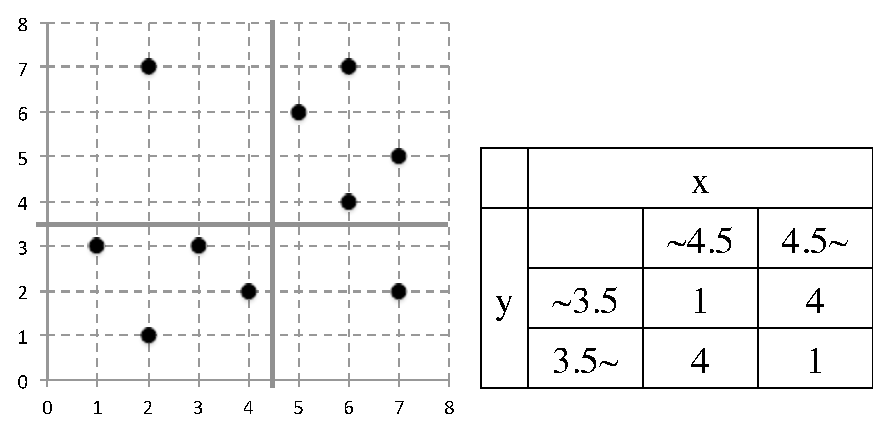
\includegraphics[scale=.50]{figure/mmbucket/split_mbucket.eps}
\end{center}
\caption{One-dimensional partition (mbucket)×2\label{fig:mmbucket_1dim}}
\end{minipage}

\begin{minipage}{0.45\hsize}
\begin{center}
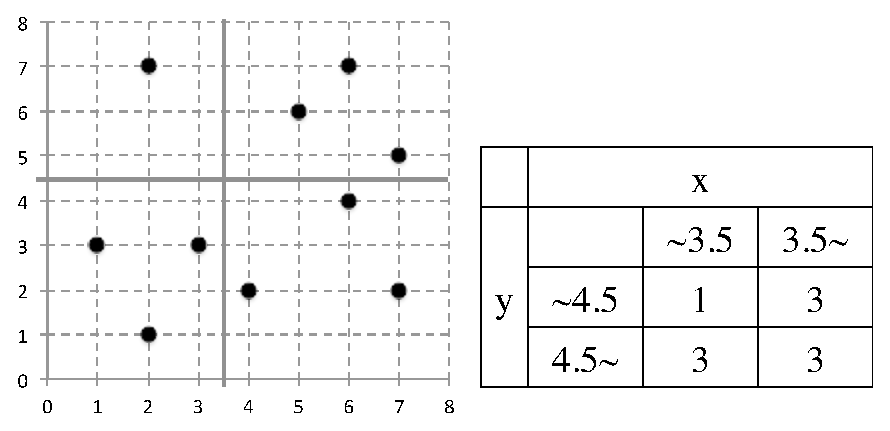
\includegraphics[scale=.50]{figure/mmbucket/split_mmbucket.eps}
\end{center}
\caption{Two-dimensional partition (mmbuket)\label{fig:mmbucket_2dim}}
\end{minipage}

\end{tabular}
\end{center}
\end{figure}


%\begin{figure}[hbt]
%\begin{center}
%\includegraphics[width=20cm,bb=0 0 738 430]{./img/bucket_var.JPG}
%\caption{1次元分割×2による分割と2次元分割による分割の比較}
%\end{center}
%\end{figure}

\subsection*{Precision experiment using on variety of fields}

The following compares the precision of mmbucket and mbucket using real data collected by \href{http://www.pmel.noaa.gov/tao/}{Tropical Atmosphere Ocean (TAO) Project}. The project is designed for the study of year-to-year climate variations related to El Nino the Southern Oscillation (ENSO), and provides provides in-situ data collection of high quality oceanographic and surface meteorological data for monitoring, forecasting, and understanding of climate swings associated with El Nino and La Nina.  Snapshot of the data is shown in the following table. \\



\begin{table}[hbt]
\begin{center}
\caption{Data set used for precision experiment }
{\footnotesize
%\begin{tabular}{p{2em}|p{2.5em}|p{2em}|p{3em}|p{3.5em}|p{4em}|p{4.5em}|p{4.5em}|p{3.5em}|p{3.5em}|p{4.5em}|p{2.5em}}\hline
\begin{tabular}{l|l|l|l|l|l|l|l|l|l|l|l}\hline
%obs  (観測id) & year (年)&month (月)&day (日)&date (日付) &latitude (緯度)&longitude (経度)&zonwinds (東西風速)	&merwinds (南北風速)&humidity (湿度)&air\_temp. (気温)&sstemp (海面温度) \\ \hline
id & year & month & day & date & latitude & longitude & zonwinds & merwinds & humidity & air\_temp. &sstemp \\ \hline
4060 & 93 &5 & 9 & 930509 & -0.02 & -109.96 & -2.1 & 2.1 & 81.2 & 26.8 & 27.02\\
4061 & 93 & 5 & 10 & 930510 & -0.02 & -109.96 & -3.4 & 1.4 & 84.2 & 26.95 & 26.91\\
4062 & 93 & 5 & 11 & 930511 & -0.02 & -109.96 & -3.8 & 2.2 & 84.9 & 26.98 & 26.78\\
4063 & 93 & 5 & 12 & 930512 & -0.02 & -109.96 & -3 & 1.5 & 86.9 & 26.93 & 26.74\\
4064 & 93 & 5 & 13 & 930513 & -0.02 & -109.96 & -4.5 & 1.9 & 87.6 & 27.01 & 26.82\\
4065 & 93 & 5 & 14 & 930514 & -0.02 & -109.96 & -5    & 1.3 & 85.6 & 26.96 & 26.68\\
\hline
\end{tabular}
\\
%latitude:緯度, longitude:経度, zonwinds:東西風速, merwinds:南北風速, humidity:湿度, air\_temp.:気温, sstemp:海面温度
}
\end{center}
\end{table}

The precision experiment uses attributes with numeric values (7 attributes from latitude to sea surface temperature) for bucket partition. The number of record rows is 93,935. Statistics for each attribute is shown in Table 3. "Types of data values" significantly affects computation time of bucket partition.


\begin{table}[hbt]
\begin{center}
\caption{Various statistics of numerical data}
{\footnotesize
\begin{tabular}{c|c|c|c|c|c|c|c} \hline
Measurement & Latitude& Longitude & Zonal wind & North-south wind & Humidity & Temp & Sea surface temp\\ \hline
Type & 482& 924& 228& 206& 385& 1104& 1201\\
Arithmetic average& 0.305& -70.8& -3.35& -0.046& 81.3& 27.1& 27.9\\
Standard deviation & 4.77& 128.7& 3.42& 3.021& 5.28& 1.674& 1.87\\
Minimum & -8.33& -180& -10.7& -10.6& 52.1& 17.5& 18.2\\
Mean & 0.01& -125& -4.1& -0.1& 81.3& 27.5& 28.4\\
Maximum& 9.05& 170.0& 14.3& 13& 99.9& 31.5& 31.0\\ \hline
\end{tabular}
}
\end{center}
\end{table}

The comparison of variance for one-dimensional bucket partition (mbucket) and two-dimensional bucket partition (mmbucket) based on a total of 21 combinations from the 7 attributes are distributed into two columns as shown in Table \ref{tbl:mmbucket_table1}. 

For example, the first row shows the comparison results of bucket partition on “temperature × humidity”, the variance of mbucket is 408274409 and the variance of mmbucket is 406438211, resulting in the ratio of (mmbucket / mbucket) 0.996. The ratio is shown for partitions of 10×10,15×15 and 20×20. The results differs according to the combination of attributes, there are minimal improvements in some combinations such as "humidity × zonal wind speed", improvements can be seen at “latitude x longtitude (15 x 15) with an improvement in accuracy of 19\% (1-0.81).

\begin{table}[hbt]
\begin{center}
\caption{Comparison of two-dimensional partition accuracy of mbucket and mmbucket\label{tbl:mmbucket_table1}}
{\footnotesize
\begin{tabular}{c|c||c|c|c|c|c|c}
\hline
% plastexにてmultirowはNG
%\multirow{2}{*}{項目1} & \multirow{2}{*}{項目2} & \multicolumn{2}{|c|}{分散値(5×5分割)} & \multicolumn{4}{|c}{分散値の比(mmbucket/mbucket)} \\  \cline{3-4}  \cline{5-8}
%                       &  & mbucket  & mmbucket & 5×5 &	10×10 & 15×15 & 20×20  \\ \hline\hline
            &          & \multicolumn{2}{|c|}{Variance (5×5 partition)} & \multicolumn{4}{|c}{Comparison of variance (mmbucket/mbucket)} \\  \cline{3-4}  \cline{5-8}
Item 1       & Item 2    & mbucket  & mmbucket & 5×5  &10×10 &15×15 & 20×20\\ \hline\hline
Temperature        & Humidity     &408274409 &406438211 &0.996 &0.987 &0.988 &0.981 \\
            & Latitude     &374125463 &371258775 &0.992 &0.988 &0.982 &0.964 \\
            & Longitude     &490727955 &454663065 &0.927 &0.949 &0.946 &0.929 \\
            & North-south wind speed &396436813 &394724219 &0.996 &0.991 &0.993 &0.989 \\
            & Sea surface temperature &816199131 &747215787 &0.915 &0.897 &0.883 &0.862 \\
            & Zonal wind speed &382069455 &381225143 &0.998 &0.998 &0.997 &0.996 \\  \hline
Temperature        & Humidity     &368492959 &367941709 &0.999 &0.994 &0.994 &0.990 \\
            & Latitude     &372116309 &370591351 &0.996 &0.991 &0.993 &0.986 \\
            & North-south wind speed &355658757 &355658757 &1.000 &1.000 &1.000 &1.000 \\
            & Sea surface temperature &380382203 &379546293 &0.998 &0.991 &0.991 &0.983 \\
            & Zonal wind speed &357729819 &357697283 &1.000 &1.000 &1.000 &1.000 \\ \hline
Latitude        & Longtitude     &365459223 &361754113 &0.990 &0.923 &0.812 &0.816 \\
            & North-south wind speed &371478669 &370970251 &0.999 &0.988 &0.985 &0.982 \\
            & Sea surface temperature &392810425 &389589403 &0.992 &0.987 &0.979 &0.952 \\
            &  Zonal wind speed &364521077 &364406663 &1.000 &0.999 &0.991 &0.992 \\ \hline
Longtitude        & Latitude &414154185 &408431667 &0.986 &0.976 &0.976 &0.962 \\
            & Sea surface temperature &510979465 &463576537 &0.907 &0.945 &0.939 &0.934 \\
            & Zonal wind speed &400021527 &392710641 &0.982 &0.983 &0.982 &0.973 \\ \hline
North-south wind    & Sea surface temperature &393233841 &392432943 &0.998 &0.995 &0.994 &0.993 \\
            & Zonal wind speed &359290669 &359074015 &0.999 &1.000 &1.000 &0.997 \\ \hline
Sea surface temp    & Zonal wind speed &442877539 &438326669 &0.990 &0.988 &0.984 &0.986 \\ \hline
\end{tabular}
}
\end{center}
\end{table}
 
\subsection*{Speed Comparison}

Next, the experiments are carried out to compare the differences in speed by against different  number of partitions. The execution time is computed using the same data “temperature × sea surface temperature” and “latitude × longitude” with 5 to 40 partitions at increments of 5.  The results are shown in Table \ref{tbl:mmbucket_table2}. The execution time of \verb|mbucket| is consistent regardless of the number of partitions. However, more time is required to compute the number of partitions for two dimensional partitions. This is due to the fact that the algorithm is not efficient in selecting multidimensional orthogonal numeric range required by computation. The partition speed will be noted as possible improvements in the next version. 


\begin{table}[hbt]
\begin{center}
\caption{Sample results of mbucket,mmbucket \label{tbl:mmbucket_table2}}
{\footnotesize
\begin{tabular}{c|c|c|c|c}
\hline
& \multicolumn{2}{|c|}{Temperature×Sea Surface Temperature} & \multicolumn{2}{|c}{Latitude×Longtitude} \\ \hline
Number of buckets &mbucket &mmbucket &mbucket &mmbucket\\ \hline
5 &0.221 &2.21 &0.216 &0.67\\
10 &0.227 &3.90 &0.216 &1.67\\
15 &0.233 &10.4 &0.230 &3.28\\
20 &0.231 &26.1 &0.228 &7.13\\
25 &0.232 &32.9 &0.237 &13.3\\
30 &0.236 &46.7 &0.236 &11.4\\
35 &0.237 &62.3 &0.240 &15.2\\
40 &0.237 &80.1 &0.237 &25.8\\ \hline
\end{tabular}
}
\end{center}
\end{table}

\subsection*{Related Command}
\hyperref[sect:mbucket]{mbucket} : This command processes one-dimensional bucket partition for each field even when more than one field is specified.

%\end{document}




%\documentclass[a4paper]{jsbook}
%\usepackage{mcmd_jp}
%\begin{document}

\section{mminput Display form input screen\label{sect:mminput}}
\index{mminput@mminput}
\underline{Note: This command is a beta. Its specifications may be changed.}

This command displays a data input screen using the text file specified by the \verb|i=| parameter as the screen form. The character strings on the screen form is displayed as is, and the area between square brackets (\verb|[]|) is shown as a freehand input field. There can be two or more input fields. The data entered by the user is output to the CSV file specified by the \verb|o=| parameter. The output data consists of one row. When there are two or more input fields, a multiple-field CSV file is output.
When the command ends with nothing entered in the input frame, null is output. To output a fieldname, use the \verb|f=| parameter. With \verb|f=| omitted, no fieldname header is output. 
The operation is indefinite if the specified coordinate is outside the scope of the terminal.

\subsection*{Format}
\verb/mminput i= [f=] /
\hyperref[sect:option_o]{o=}
\hyperref[sect:option_nfn]{[-nfn]} 
\hyperref[sect:option_nfno]{[-nfno]}  
\hyperref[sect:option_x]{[-x]}
\verb|[--help]|
\verb|[--helpl]|
\verb|[--version]|\\

\subsection*{Parameters}
\begin{table}[htbp]
%\begin{center}
{\small
\begin{tabular}{ll}
\verb|i=| & Specify the text file containing the screen form.\\
\verb|f=| & Specify the output fieldname.\\
\end{tabular} 
}
\end{table} 

\subsection*{Examples}

\subsubsection*{Example 1: Basic example}
A \verb|name| and \verb|address| input screen is displayed. The entered name and address are output to \verb|rsl1.csv| under fieldnames name,address.

\begin{Verbatim}[baselinestretch=0.7,frame=single]
$ more screen.txt

     name   :[               ]
     address:[               ]

$ mminput i=screen.txt f=name,address o=rsl1.csv
$ more rsl1.csv
name,address
Taro,Japan


The following will be displayed:
+--------------------------------------
|
|     name   :[Taro           ]
|     address:[Japan          ]
|
\end{Verbatim}

\subsubsection*{Example 2: Judging end status}
The parameters are the same as in Example 1. This script judges the end status and performs different operations accordingly.

\begin{Verbatim}[baselinestretch=0.7,frame=single]
$ more scp.sh
rm -f rsl3.csv
clear
mminput i=screen.txt f=name,address o=rsl3.csv
if [ $? = 0 ] ; then
  clear ; echo "end by enter key"
else
  clear ; echo "end by escape key"
fi

# Result of typing Taro and Japan and pressing Enter
$ bash scp.sh
end by enter key
$ more rsl3.csv
name,address
Taro,Japan

# Result of typing Taro and Japan and pressing ESC
$ bash scp.sh
end by escape key
$ more rsl3.csv
name,address
Taro,Japan
\end{Verbatim}

\subsection*{Related Commands}
\hyperref[sect:minput] {minput} : Displays the input screen.
\hyperref[sect:mdsp] {mdsp} : Displays a character string at the specified position on the screen.
\hyperref[sect:mseldsp] {mseldsp} : Displays a single-choice input window on the screen.
\hyperref[sect:mmseldsp] {mmseldsp} : Displays a multiple-choice input window on the screen.

%\end{document}


%\documentclass[a4paper]{jsbook}
%\usepackage{mcmd_jp}
%\begin{document}

\section{mmseldsp 複数選択画面入力\label{sect:mmseldsp}}
\index{mmseldsp@mmseldsp}
\underline{注)本コマンドは開発バージョンであり、仕様が変更される可能性があります。}

座標\verb|x=,y=|で指定したターミナル上の位置に\verb|i=|、
もしくは\verb|seldata=|で指定した文字列リストの選択画面を表示し、
ユーザが選んだ文字列を\verb|o=|で指定したファイルに出力する。
\hyperref[sect:mseldsp]{mseldsp}コマンドでは、利用者は一つの選択肢しか選択できないが、
\verb|mmseldsp|は複数の選択肢を選択できる。
選ばれた複数の文字列は、複数行のCSV項目として出力される。
入力枠に何も入力せずに終了した場合は、null値が出力される(すなわち改行だけが出力される)。
\verb|f=|を指定すれば、項目名を出力できる。
\verb|f=|を省略すれば、項目名ヘッダーは出力されない。
選択肢の数が多くて画面をはみ出る場合は、\verb|height=|で
スクロール窓の行数を指定すればよい。

選択画面でエンターキーを押すと、終了ステータス0を返して終了し、
エスケープキーを押すと、終了ステータス1を返して終了する。
いずれのキーで終了しても、選択画面で選ばれた内容はファイルに出力される。

座標は左上が\verb|x=1,y=1|である(エスケープシーケンスの仕様)。
\verb|x=|もしくは\verb|y=|で指定した値が1より小さい場合は、1を指定したものとして動作する。
またターミナルの範囲を超えた座標が指定された場合の動作は不定である。


\subsection*{書式}
\verb/mmseldsp x= y= [f=] [height=] i=|seldata=/
\hyperref[sect:option_o]{o=}
\hyperref[sect:option_nfn]{[-nfn]} 
\hyperref[sect:option_nfno]{[-nfno]}  
\hyperref[sect:option_x]{[-x]}
\hyperref[sect:option_option_tmppath]{[tmpPath=]}
\hyperref[sect:option_precision]{[precision=]}
\verb|[-params]|
\verb|[--help]|
\verb|[--helpl]|
\verb|[--version]|\\

\subsection*{パラメータ}
\begin{table}[htbp]
%\begin{center}
{\small
\begin{tabular}{ll}
\verb|o=|   & 出力ファイル名を指定する。\\
\verb|x=|   & x軸(左から右への横方向)表示開始位置(1以上の値)を指定する。\\
\verb|y=|   & y軸(上から下への縦方向)表示開始位置(1以上の値)を指定する。\\
\verb|height=| & 選択肢を表示する行数。 \\
\verb|i=|   & 選択肢の文字列を項目として持つCSVファイル名 \\
\verb|f=|   & 選択肢の文字列を項目として持つCSVファイル名 \\
\verb|seldata=| & カンマで区切られた選択肢の文字列リスト \\
\end{tabular} 
}
\end{table} 

\subsection*{利用例}

\subsubsection*{例1: 基本例}

ターミナルのx=10,y=2の位置に\verb|sel.txt|の内容を表示し、
利用者が選んだ文字列を\verb|rsl1.txt|に出力する。

\begin{Verbatim}[baselinestretch=0.7,frame=single,commandchars=\\\{\}]
$ more sel.txt
apple
pineapple
grape
orange
$ mmseldsp x=10 y=2 i=sel.txt o=rsl1.txt
# 利用者が一行目を選んだとする。
$ mose rsl1.txt
apple
orange


以下、画面イメージ
+--------------------------------------
|
|          \textColor{red}{black}{apple    }
|          \textColor{white}{black}{pineapple}
|          \textColor{white}{black}{grape}
|          \textColor{red}{black}{orange   }
|
\end{Verbatim}

\subsubsection*{例2: 引数で与える例}

例1と同様で、選択肢の文字列を\verb|seldata=|で与える。

\begin{Verbatim}[baselinestretch=0.7,frame=single,commandchars=\\\{\}]
$ mmseldsp x=10 y=2 seldata=apple,pineapple,grape,orange o=rsl2.txt
# 利用者が二行目を選んだとする。
$ mose rsl2.txt
apple
grape


以下、画面イメージ
+--------------------------------------
|
|
|          \textColor{red}{black}{apple    }
|          \textColor{white}{black}{pineapple}
|          \textColor{red}{black}{grape    }
|          \textColor{white}{black}{orange}
|
\end{Verbatim}

\subsubsection*{例3: 終了ステータスを判定する例}

例2と同じパラメータで実行し、終了ステータスを判定して異なる動作をするスクリプトの例。

\begin{Verbatim}[baselinestretch=0.7,frame=single]
$ more scp.sh
rm -f rsl3.csv
clear
mmseldsp x=10 y=2 seldata=apple,pineapple,grape,orange o=rsl3.csv
if [ $? = 0 ] ; then
  clear ; echo "end by enter key"
else
  clear ; echo "end by escape key"
fi

# appleを選択後enterキーを入力した場合の結果
$ bash scp.sh
end by enter key
$ more rsl3.csv
apple

# appleを選択後escapeキーを入力した場合の結果
$ bash scp.sh
end by escape key
$ more rsl3.csv
apple
\end{Verbatim}

\subsection*{関連コマンド}
\hyperref[sect:minput] {minput} :入力画面を表示する。

\hyperref[sect:mminput] {mminput} : 複数入力枠による入力画面を表示する。

\hyperref[sect:mdsp] {mdsp} : 画面の指定位置に文字列を表示する。

\hyperref[sect:mseldsp] {mseldsp} : 画面に単一選択入力窓を表示する。


%\end{document}


%\begin{document}

\section{mmvavg - Calculate Moving Average\label{sect:mmvavg}}
\index{mmvavg@mmvavg}

Calculate the moving average. The three different ways to calculate moving average include simple moving average ($SMA$), weighted moving average ($WMA$), and exponential moving average ($EMA$). 


\if0 #no help# following sentences will not apear on the help document. \fi

The value of $t$ time is expressed by $x_t$, and period is represented by $m$ as defined in several formulas of moving average (\ref{eq:sma},\ref{eq:wma},\ref{eq:ema}).


\begin{eqnarray}
%\begin{footnotesize}
SMA_t=\frac{1}{m} \sum_{i=0}^{m-1} x_{t-i}
\label{eq:sma}
%\end{footnotesize}
\end{eqnarray}

\begin{eqnarray}
%\begin{footnotesize}
WMA_t=\sum_{i=0}^{m-1} \frac{m-i}{S} x_{t-i},\ \ S=\sum_{i=1}^m i
\label{eq:wma}
%\end{footnotesize}
\end{eqnarray}

\begin{eqnarray}
%\begin{footnotesize}
EMA_t=\alpha x_t + (1-\alpha)EMA_{t-1}
\label{eq:ema}
%\end{footnotesize}
\end{eqnarray}

\subsection*{Format}
\verb/mmvavg [s=] [k=] [n=] f= [t=] [-exp|-w] [alpha=] [skip=]/
\hyperref[sect:option_i]{[i=]}
\hyperref[sect:option_o]{[o=]}
\hyperref[sect:option_assert_diffSize]{[-assert\_diffSize]}
\hyperref[sect:option_assert_nullkey]{[-assert\_nullkey]}
\hyperref[sect:option_assert_nullin]{[-assert\_nullin]}
\hyperref[sect:option_assert_nullout]{[-assert\_nullout]}
\hyperref[sect:option_nfn]{[-nfn]} 
\hyperref[sect:option_nfno]{[-nfno]}  
\hyperref[sect:option_x]{[-x]}
\hyperref[sect:option_q]{[-q]}
\hyperref[sect:option_option_tmppath]{[tmpPath=]}
\hyperref[sect:option_precision]{[precision=]}
\verb|[--help]|
\verb|[--helpl]|
\verb|[--version]|\\

\subsection*{Parameters}
\begin{table}[htbp]
%\begin{center}
{\small
\begin{tabular}{ll}
\verb|s=|    & After the specified field is sorted (multiple fields can be specified), moving average is calculated. \\
             & \verb|s=| parameter is required when \verb|-q| option is not specified. \\
\verb|k=|    & Aggregate records using the specified field name(s) (multiple fields can as unit of calculation. \\
\verb|f=|    & Compute the moving averages of the field(s) (multiple fields can be specified). \\
\verb|t=|    & Interval numbers of integers greater than 1.  \\
             & When \verb|-exp| is used with \verb|alpha=|, the \verb|t=| parameter do not need to be defined. \\
\verb|-w|    & Linear weighted moving average.\\
\verb|-exp|  & Exponential smoothing moving average. \\
\verb|alpha=|& Use a real number as smoothing coefficient when \verb|-exp| is specified. \\
             & The default value of alpha is \verb|alpha=2/(value of = t+1)|。\\
\verb|skip=| & Specify the number of rows to hide from the top in the output. \\
             & Default value: \verb|skip=(value of t= -1)|, \verb|skip=0| when \verb|-exp| is specified.  \\
\end{tabular} 
}
\end{table} 


\subsection*{Examples}
\subsubsection*{Example 1: Basic Example}

The first row is not printed as there is less than the number of required intervals for computation.


\begin{Verbatim}[baselinestretch=0.7,frame=single]
$ more dat1.csv
id,value
1,5
2,1
3,3
4,4
5,4
6,6
7,1
8,4
9,7
$ mmvavg s=id f=value t=2 i=dat1.csv o=rsl1.csv
#END# kgmvavg f=value i=dat1.csv o=rsl1.csv s=id t=2
$ more rsl1.csv
id%0,value
2,3
3,2
4,3.5
5,4
6,5
7,3.5
8,2.5
9,5.5
\end{Verbatim}
\subsubsection*{Example 2: Basic Example 2}

The first row is not printed as there is less than the number of required intervals for computation.


\begin{Verbatim}[baselinestretch=0.7,frame=single]
$ mmvavg s=id f=value t=2 -w i=dat1.csv o=rsl2.csv
#END# kgmvavg -w f=value i=dat1.csv o=rsl2.csv s=id t=2
$ more rsl2.csv
id%0,value
2,2.333333333
3,2.333333333
4,3.666666667
5,4
6,5.333333333
7,2.666666667
8,3
9,6
\end{Verbatim}
\subsubsection*{Example 3: Basic Example 3}

Exponential smoothing moving average (\verb|-exp|) includes the first row in the output.


\begin{Verbatim}[baselinestretch=0.7,frame=single]
$ mmvavg s=id f=value t=2 -exp i=dat1.csv o=rsl3.csv
#END# kgmvavg -exp f=value i=dat1.csv o=rsl3.csv s=id t=2
$ more rsl3.csv
id%0,value
1,5
2,2.333333333
3,2.777777778
4,3.592592593
5,3.864197531
6,5.288065844
7,2.429355281
8,3.47645176
9,5.82548392
\end{Verbatim}
\subsubsection*{Example 4: An example of assigning key}



\begin{Verbatim}[baselinestretch=0.7,frame=single]
$ more dat2.csv
id,key,value
1,a,5
2,a,1
3,a,3
4,a,4
5,a,4
6,b,6
7,b,1
8,b,4
9,b,7
$ mmvavg s=key,id k=key f=value t=2 i=dat2.csv o=rsl4.csv
#END# kgmvavg f=value i=dat2.csv k=key o=rsl4.csv s=key,id t=2
$ more rsl4.csv
id,key,value
2,a,3
3,a,2
4,a,3.5
5,a,4
7,b,3.5
8,b,2.5
9,b,5.5
\end{Verbatim}
\subsubsection*{Example 5: Display all records including those that are less than the defined intervals }



\begin{Verbatim}[baselinestretch=0.7,frame=single]
$ more dat3.csv
key,value
a,1
a,2
a,3
a,4
a,5
b,6
b,1
b,4
b,7
$ mmvavg -q k=key f=value t=2 skip=0 i=dat3.csv o=rsl5.csv
#END# kgmvavg -q f=value i=dat3.csv k=key o=rsl5.csv skip=0 t=2
$ more rsl5.csv
key,value
a,1
a,1.5
a,2.5
a,3.5
a,4.5
b,6
b,3.5
b,2.5
b,5.5
\end{Verbatim}

\subsection*{Related Commands}
\hyperref[sect:mmvstats] {mmvstats} : Specify the average as well as various types of statistics. 

\hyperref[sect:mmvsim] {mmvsim} : Compute bivariate statistics. 

\hyperref[sect:mwindow] {mwindow} : Computes statistics on sliding window data which cannot be computed using \verb|mmvstats|. 

%\end{document}


%\documentclass[a4paper]{jsbook}
%\usepackage{mcmd_jp}
%\begin{document}

\section{mmvsim 移動窓の類似度計算\label{sect:mmvsim}}
\index{mmvsim@mmvsim}

移動窓を設定し、各種類似度(2変量の統計量)を計算する。
\hyperref[sect:msim]{msim}コマンドの移動窓バージョンとして考えればよい。
\verb|msim|との違いは、指定できる類似度は一つだけで、また類似度計算の対象項目は2つのみである。

\subsection*{書式}
\verb|mmvsim [s=] [k=] f= c= a= [t=] [skip=] [-n] |
\hyperref[sect:option_i]{[i=]}
\hyperref[sect:option_o]{[o=]}
\hyperref[sect:option_assert_diffSize]{[-assert\_diffSize]}
\hyperref[sect:option_assert_nullkey]{[-assert\_nullkey]}
\hyperref[sect:option_assert_nullin]{[-assert\_nullin]}
\hyperref[sect:option_assert_nullout]{[-assert\_nullout]}
\hyperref[sect:option_nfn]{[-nfn]} 
\hyperref[sect:option_nfno]{[-nfno]}  
\hyperref[sect:option_x]{[-x]}
\hyperref[sect:option_q]{[-q]}
\hyperref[sect:option_option_tmppath]{[tmpPath=]}
\hyperref[sect:option_precision]{[precision=]}
\verb|[-params]|
\verb|[--help]|
\verb|[--helpl]|
\verb|[--version]|\\

\subsection*{パラメータ}
\begin{table}[htbp]
%\begin{center}
{\small
\begin{tabular}{ll}
\verb|i=|    & 入力ファイル名を指定する。\\
\verb|o=|    & 出力ファイル名を指定する。\\
\verb|s=|    & ここで指定した項目(複数項目指定可)で並べ替えられた後、各種類似度が計算される。\\
             & \verb|-q|オプションを指定しないとき、\verb|s=|パラメータは必須。\\
\verb|k=|    & ここで指定された項目(複数項目指定可)を単位として集計する。 \\
\verb|f=|    & 集計項目名リスト(複数項目指定可)を指定する。\\
\verb|t=|    & 期間数を1以上の整数で指定する。 \\
\verb|c=|    & 類似度(以下のリストから一つだけ)指定する。\\
             & \verb/covar|ucovar|pearson|spearman|kendall|euclid|/\\
             & \verb/cosine|cityblock|hamming|chi|phi|jaccard|support|lift/ \\
             & 詳細な定義は\hyperref[sect:msim]{msim}コマンドを参照のこと。\\
\verb|skip=| & 出力を抑制する最初の行数を指定する。【デフォルト値:\verb|skip=(t=の値-1)|】\\
\verb|a=| & 計算結果の出力として追加される項目の名前を指定する。 \\
\verb|-n| & 期間内にNULL値が1つでも含まれていると結果もNULL値とする。\\
\end{tabular} 
}
\end{table} 

\subsection*{利用例}
\subsubsection*{例1: 基本例}

\verb|x、y|項目についてのピアソンの積率相関係数を3期を窓として計算する。


\begin{Verbatim}[baselinestretch=0.7,frame=single]
$ more dat1.csv
t,x,y
1,14,0.17
2,11,0.2
3,32,0.15
4,13,0.33
5,8,0.1
6,19,0.56
$ mmvsim s=t t=3 c=pearson f=x,y a=sim i=dat1.csv o=rsl1.csv
#END# kgmvsim a=sim c=pearson f=x,y i=dat1.csv o=rsl1.csv s=t t=3
$ more rsl1.csv
t%0,x,y,sim
3,32,0.15,-0.8746392857
4,13,0.33,-0.6515529194
5,8,0.1,-0.1164257338
6,19,0.56,0.9986254289
\end{Verbatim}


\subsection*{関連コマンド}
\hyperref[sect:msim] {msim} : 移動窓を設定せずに類似度計算を行う。

\hyperref[sect:mwindow] {mwindow} : 動窓のデータを作成するので、そのデータを使えば\verb|mmvstats|で計算できない統計量も計算可能。

\hyperref[sect:mmvavg] {mmvavg} : 移動平均に限定した計算を行う。

%\end{document}


%\documentclass[a4paper]{jsbook}
%\usepackage{mcmd_jp}
%\begin{document}

\section{mmvstats 移動窓の統計量の計算\label{sect:mmvstats}}
\index{mmvstats@mmvstats}

移動窓を設定し、各種統計量(1変量)を計算する。
\hyperref[sect:mstats]{mstats}コマンドの移動窓バージョンとして考えればよい。

\subsection*{書式}
\verb|mmvstats [s=] [k=] f= [t=] c= [skip=] -n |
\hyperref[sect:option_i]{[i=]}
\hyperref[sect:option_o]{[o=]}
\hyperref[sect:option_assert_diffSize]{[-assert\_diffSize]}
\hyperref[sect:option_assert_nullkey]{[-assert\_nullkey]}
\hyperref[sect:option_assert_nullin]{[-assert\_nullin]}
\hyperref[sect:option_assert_nullout]{[-assert\_nullout]}
\hyperref[sect:option_nfn]{[-nfn]} 
\hyperref[sect:option_nfno]{[-nfno]}  
\hyperref[sect:option_x]{[-x]}
\hyperref[sect:option_q]{[-q]}
\hyperref[sect:option_option_tmppath]{[tmpPath=]}
\hyperref[sect:option_precision]{[precision=]}
\verb|[-params]|
\verb|[--help]|
\verb|[--helpl]|
\verb|[--version]|\\

\subsection*{パラメータ}
\begin{table}[htbp]
%\begin{center}
{\small
\begin{tabular}{ll}
\verb|i=|    & 入力ファイル名を指定する。\\
\verb|o=|    & 出力ファイル名を指定する。\\
\verb|s=|    & ここで指定した項目(複数項目指定可)で並べ替えられた後、各種統計量が計算される。\\
             & \verb|-q|オプションを指定しないとき、\verb|s=|パラメータは必須。\\
\verb|k=|    & ここで指定された項目(複数項目指定可)を単位として集計する。\\
\verb|f=|    & 集計項目名リスト(複数項目指定可)を指定する。\\
\verb|t=|    & 期間数を1以上の整数で指定する。 \\
\verb|c=|    & 統計量(以下のリストから一つだけ指定可)\\
             & \verb/sum|mean|devsq|var|uvar|sd|usd|cv|min|/\\
             & \verb/|max|range|skew|uskew|kurt|ukurt/\\
             & 詳細な定義は\hyperref[sect:mstats]{mstats}コマンドを参照のこと。\\
\verb|skip=| & 出力を抑制する最初の行数\\
\verb|-n| & 期間内にNULL値が1つでも含まれていると結果もNULL値とする。\\
\end{tabular} 
}
\end{table} 


\subsection*{利用例}
\subsubsection*{Example 1: Basic Example}

Calculate sum of sliding window.
The first row is not printed as there is less than the required nubmer of intervals for computation.


\begin{Verbatim}[baselinestretch=0.7,frame=single]
$ more dat1.csv
id,value
1,5
2,1
3,3
4,4
5,4
6,6
7,1
8,4
9,7
$ mmvstats s=id f=value t=2 c=sum i=dat1.csv o=rsl1.csv
#END# kgmvstats c=sum f=value i=dat1.csv o=rsl1.csv s=id t=2
$ more rsl1.csv
id%0,value
2,6
3,4
4,7
5,8
6,10
7,7
8,5
9,11
\end{Verbatim}

\subsection*{関連コマンド}
\hyperref[sect:mmvavg] {mmvavg} : 移動平均に限定した計算を行う。

\hyperref[sect:mwindow] {mwindow} : 動窓のデータを作成するので、そのデータを使えば\verb|mmvstats|で計算できない統計量も計算可能。

\hyperref[sect:mmvsim] {mmvsim} : 移動窓の類似度(2変量統計量)の計算を行う。

%\end{document}


%\documentclass[a4paper]{jsbook}
%\usepackage{mcmd_jp}
%\begin{document}

\section{mnewnumber 連番データの新規生成\label{sect:mnewnumber}}
\index{mnewnumber@mnewnumber}
\verb|S=|パラメータで指定した開始数値もしくはアルファベットにより、
\verb|I=|パラメータで指定した間隔で連番もしくはアルファベット連番を新規作成し、\verb|a=|パラメータで指定した項目名で出力する。
アルファベット連番とは、AからZの26文字を用いた26進数のこと(A,B,$\cdots$,Z,AA,AB,$\cdots$,AZ,BA,BB,$\cdots$,ZZ,AAA,AAB,$\cdots$)。

\subsection*{書式}
\verb|mnewnumber a= [I=] [S=] [l=]|
\hyperref[sect:option_o]{[o=]}
\hyperref[sect:option_nfn]{[-nfn]} 
\hyperref[sect:option_nfno]{[-nfno]}  
\hyperref[sect:option_x]{[-x]}
\hyperref[sect:option_option_tmppath]{[tmpPath=]}
\hyperref[sect:option_precision]{[precision=]}
\verb|[-params]|
\verb|[--help]|
\verb|[--helpl]|
\verb|[--version]|\\

\subsection*{パラメータ}
\begin{table}[htbp]
%\begin{center}
{\small
\begin{tabular}{ll}
\verb|o=|    & 出力ファイル名を指定する。\\
\verb|a=|    & 新規に作成する連番行の項目名を指定する。\\
             & \verb|-nfn,-nfno|オプション指定時は指定の必要はない。\\
\verb|I=|    & 連番をふる間隔を指定する。【デフォルト値:1】\\
\verb|S=|    & 開始数値/アルファベット(大文字)【デフォルト値:1】\\
             & 連番の開始数値もしくはアルファベットを指定する。\\
             & 数値を指定した場合は数値の連番がふられる。\\
             & アルファベットを指定した場合はアルファベット連番がふられる。(小文字は指定できない)\\
\verb|l=|    & 作成するデータ行数を指定する。【デフォルト値:10】\\
\end{tabular} 
}
\end{table} 


\subsection*{利用例}
\subsubsection*{Example 1: Basic Example}

Generate a dataset with 5 sequential numbers starting from 1 incremented by 1. Name the sequence as \verb|No.|.


\begin{Verbatim}[baselinestretch=0.7,frame=single]
$ mnewnumber a=No. I=1 S=1 l=5 o=rsl1.csv
#END# kgNewnumber I=1 S=1 a=No. l=5 o=rsl1.csv
$ more rsl1.csv
No.
1
2
3
4
5
\end{Verbatim}
\subsubsection*{Example 2: Change the starting number and interval }

Generate a dataset consisting of 5 sequential numbers starting from 10 with an incremental interval of 5. Name the sequence as \verb|No.|.


\begin{Verbatim}[baselinestretch=0.7,frame=single]
$ mnewnumber a=No. I=5 S=10 l=5 o=rsl2.csv
#END# kgNewnumber I=5 S=10 a=No. l=5 o=rsl2.csv
$ more rsl2.csv
No.
10
15
20
25
30
\end{Verbatim}
\subsubsection*{Example 3: Generate series of alphabet}

Generate a dataset consisting of 5 alphabet sequence starting from A with 1 alphabet in between. Name the sequence as \verb|No.|.


\begin{Verbatim}[baselinestretch=0.7,frame=single]
$ mnewnumber a=No. I=1 S=A l=5 o=rsl3.csv
#END# kgNewnumber I=1 S=A a=No. l=5 o=rsl3.csv
$ more rsl3.csv
No.
A
B
C
D
E
\end{Verbatim}
\subsubsection*{Example 4: Generate data without header}

Generate a dataset consisting of 11 alphabet sequence starting from B with 3 alphabets in between. Exclude the header from the output.


\begin{Verbatim}[baselinestretch=0.7,frame=single]
$ mnewnumber  -nfn  I=3 l=11 S=B o=rsl4.csv
#END# kgNewnumber -nfn I=3 S=B l=11 o=rsl4.csv
$ more rsl4.csv
B
E
H
K
N
Q
T
W
Z
AC
AF
\end{Verbatim}


\subsection*{関連コマンド}
\hyperref[sect:mnewrand] {mnewrand} : 新たに乱数を生成する。

\hyperref[sect:mnewstr] {mnewstr} : 固定文字列を生成する。

%\end{document}


%\begin{document}

\section{mnewrand 乱数データの新規生成\label{sect:mnewrand}}
\index{mnewrand@mnewrand}
0.0から1.0の範囲の実数乱数を生成する。
\verb|-int|を指定することで、整数乱数を生成することもできる。

乱数の生成にはメルセンヌ・ツイスター法を利用している
(\href{http://www.math.sci.hiroshima-u.ac.jp/~m-mat/MT/emt.html}{原作者のページ}
, \href{http://www.boost.org/doc/libs/1_54_0/doc/html/boost_random.html}{boostライブラリ})。


\subsection*{書式}
\verb|mnewrand a= [max=] [min=] [S=] [l=] [-int]|
\hyperref[sect:option_o]{[o=]}
\hyperref[sect:option_nfn]{[-nfn]} 
\hyperref[sect:option_nfno]{[-nfno]}  
\hyperref[sect:option_x]{[-x]}
\hyperref[sect:option_option_tmppath]{[tmpPath=]}
\hyperref[sect:option_precision]{[precision=]}
\verb|[-params]|
\verb|[--help]|
\verb|[--helpl]|
\verb|[--version]|\\

\subsection*{パラメータ}
\begin{table}[htbp]
%\begin{center}
{\small
\begin{tabular}{ll}
\verb|o=|      & 出力ファイル名を指定する。\\
\verb|a=|      & 新規に作成するデータの項目名を指定する。\\
               & \verb|-nfn,-nfno|オプション指定時は指定の必要はない。\\
\verb|max=|    & 乱数の最大値を指定する。【デフォルト値:INT\_MAX】\\
               & このパラメータを指定するときは\verb|-int|も指定しなければならない。\\
\verb|min=|    & 乱数の最小値を指定する。【デフォルト値:0】\\
               & このパラメータを指定するときは\verb|-int|も指定しなければならない。\\
\verb|S=|      & 乱数の種を指定する。【デフォルト値:現在時刻】\\
\verb|l=|      & 行数【デフォルト値:10】\\
               & 新規作成する乱数データの行数を指定する。\\
\verb|-int|    & 整数乱数を生成する\\
\end{tabular} 
}
\end{table} 


\subsection*{利用例}
\subsubsection*{例1: 基本例}

実数乱数を10行生成する。乱数の種は1に固定しているので、いつ実行しても乱数系列は同じになる。


\begin{Verbatim}[baselinestretch=0.7,frame=single]
$ mnewrand a=rand S=1 o=rsl1.csv
#END# kgnewrand S=1 a=rand o=rsl1.csv
$ more rsl1.csv
rand
0.4170219984
0.9971848081
0.7203244893
0.9325573612
0.0001143810805
0.1281244478
0.3023325677
0.9990405154
0.1467558926
0.2360889763
\end{Verbatim}
\subsubsection*{例2: 整数乱数}

最小値が0、最大値が1000、乱数の種が1の整数乱数を5行作成する。


\begin{Verbatim}[baselinestretch=0.7,frame=single]
$ mnewrand a=rand -int max=1000 min=0 l=5 S=1 o=rsl2.csv
#END# kgnewrand -int S=1 a=rand l=5 max=1000 min=0 o=rsl2.csv
$ more rsl2.csv
rand
417
998
721
933
0
\end{Verbatim}
\subsubsection*{例3: ヘッダ行なしで出力}

\verb|-nfn|でヘッダーなしのデータが生成される。


\begin{Verbatim}[baselinestretch=0.7,frame=single]
$ mnewrand -nfn l=5 S=1 o=rsl3.csv
#END# kgnewrand -nfn S=1 l=5 o=rsl3.csv
$ more rsl3.csv
0.4170219984
0.9971848081
0.7203244893
0.9325573612
0.0001143810805
\end{Verbatim}


\subsection*{関連コマンド}
\hyperref[sect:mnewnumber] {mnewnumber} : 連番を生成する。

\hyperref[sect:mnewstr] {mnewstr} : 固定文字列を生成する。

%\end{document}


%\begin{document}

\section{mnewstr 固定文字列データの新規生成\label{sect:mnewstr}}
\index{mnewstr@mnewstr}
\verb|v=|パラメータで指定した文字列データを新規作成し、\verb|a=|パラメータで指定した項目名で出力する。
一度に複数の項目を生成することも可能。

\subsection*{書式}
\verb|mnewstr a= [v=] [l=]|
\hyperref[sect:option_o]{[o=]}
\hyperref[sect:option_nfn]{[-nfn]} 
\hyperref[sect:option_nfno]{[-nfno]}  
\hyperref[sect:option_x]{[-x]}
\hyperref[sect:option_option_tmppath]{[tmpPath=]}
\hyperref[sect:option_precision]{[precision=]}
\verb|[-params]|
\verb|[--help]|
\verb|[--helpl]|
\verb|[--version]|\\

\subsection*{パラメータ}
\begin{table}[htbp]
%\begin{center}
{\small
\begin{tabular}{ll}
\verb|o=|    & 出力ファイル名を指定する。\\
\verb|a=|    & 新規に作成するデータの項目名を指定する。\\
             & 複数の項目を生成する場合は、項目名をカンマで区切る。\\
             & \verb|-nfn,-nfno|オプション指定時は指定の必要はない。\\
\verb|v=|    & 新しく作成する文字列を指定する。\\
             & 複数の項目を生成する場合は、値をカンマで区切る。\verb|a=|で指定した個数と同数でなければならない。\\
\verb|l=|    & 新規作成する乱数データの行数を指定する。【デフォルト値:10】\\
\end{tabular} 
}
\end{table} 


\subsection*{利用例}
\subsubsection*{例1: 基本例}

\verb|custNo|と\verb|A0001|という文字列データを5行作成し、\verb|attribute,code|という名前の項目名で出力する。


\begin{Verbatim}[baselinestretch=0.7,frame=single]
$ mnewstr a=attribute,code v=custNo,A0001 l=5 o=rsl1.csv
#END# kgnewstr a=attribute,code l=5 o=rsl1.csv v=custNo,A0001
$ more rsl1.csv
attribute,code
custNo,A0001
custNo,A0001
custNo,A0001
custNo,A0001
custNo,A0001
\end{Verbatim}

\subsection*{関連コマンド}
\hyperref[sect:mnewnumber] {mnewnumber} : 連番を生成する。

\hyperref[sect:mnewrand] {mnewrand} : 乱数を生成する。

%\end{document}


%\documentclass[a4paper]{jsbook}
%\usepackage{mcmd_jp}
%\begin{document}

\section{mnjoin 参照ファイル項目の自然結合\label{sect:mnjoin}}
\index{mnjoin@mnjoin}
\verb|k=|パラメータで指定した入力ファイルの項目値と参照ファイルの項目値を比較し、
同じ値の場合\verb|m=|パラメータで指定した参照ファイルにある
\verb|f=|パラメータで指定した項目値を自然結合する。 
\verb|mjoin|コマンドとの違いは、参照ファイル上のキー項目に重複があってもよい点である。
あるキー値について、入力ファイル上に$n$件、参照ファイル上に$m$件のレコードがあった場合、
$n\times m$件のレコードが出力されることになる。
また、\verb|f=|を省略すると、参照ファイルのキー項目以外全ての項目を結合する。

\subsection*{書式}
\verb/mnjoin k= [f=] [K=] [-n] [-N] m=|/ 
\hyperref[sect:option_i]{i=}
\hyperref[sect:option_o]{[o=]}
\hyperref[sect:option_bufcount]{[bufcount=]} 
\hyperref[sect:option_assert_diffSize]{[-assert\_diffSize]}
\hyperref[sect:option_assert_nullkey]{[-assert\_nullkey]}
\hyperref[sect:option_assert_nullin]{[-assert\_nullin]}
\hyperref[sect:option_assert_nullout]{[-assert\_nullout]}
\hyperref[sect:option_nfn]{[-nfn]} 
\hyperref[sect:option_nfno]{[-nfno]}  
\hyperref[sect:option_x]{[-x]}
\hyperref[sect:option_q]{[-q]}
\hyperref[sect:option_option_tmppath]{[tmpPath=]}
\hyperref[sect:option_precision]{[precision=]}
\verb|[-params]|
\verb|[--help]|
\verb|[--helpl]|
\verb|[--version]|\\

\subsection*{パラメータ}
\begin{table}[htbp]
%\begin{center}
{\small
\begin{tabular}{ll}
\verb|i=|    & 入力ファイル名を指定する。\\
\verb|o=|    & 出力ファイル名を指定する。\\
\verb|k=|    & 入力データ上の突き合わせる項目名リストを指定する。\\
             & ここで指定した入力データの項目と\verb|K=|パラメータで指定された \\
             & 参照データの項目が同じ行の項目結合が行われる。\\
\verb|f=|    & 結合する参照ファイル上の項目名リストを指定する。\\
             & 省略するとキー項目を除いた全ての項目が結合される。\\
\verb|m=|    & 参照ファイル名を指定する。\\
             & このパラメータが省略された時には標準入力が用いられる。(\verb|i=|指定ありの場合)\\
\verb|K=|    & 参照データ上の突き合わせる項目名リスト\\
             & ここで指定した参照データの項目と\verb|k=|パラメータで指定された
               入力データの項目が同じ行の項目結合が行われる。\\
             & 参照データ上に\verb|k=|パラメータで指定した入力データ上の
               項目と同名の項目が存在する場合は指定する必要はない。\\
\verb|bufcount=| & バッファのサイズ数を指定する。 \\
\verb|-n|    & 参照データにない入力データをNULL値として出力するフラグ。\\
\verb|-N|    & 入力データにない参照データをNULL値として出力するフラグ。\\
\end{tabular} 
}
\end{table} 

\subsection*{利用例}
\subsubsection*{例1: 基本例}

入力ファイルにある\verb|item|項目と、
参照ファイルにある\verb|item|項目を比較し同じ値の場合、\verb|cost|項目を結合する。
入力ファイル、参照ファイル共に\verb|item=A|が2行あり、結果、出力ファイルには2$\times$2=4行の\verb|item=A|が出力されている。


\begin{Verbatim}[baselinestretch=0.7,frame=single]
$ more dat1.csv
item,date,price
A,20081201,100
A,20081213,98
B,20081002,400
B,20081209,450
C,20081201,100
$ more ref1.csv
item,cost
A,50
A,70
B,300
E,200
$ mnjoin k=item f=cost m=ref1.csv i=dat1.csv o=rsl1.csv
#END# kgnjoin f=cost i=dat1.csv k=item m=ref1.csv o=rsl1.csv
$ more rsl1.csv
item%0,date,price,cost
A,20081201,100,50
A,20081201,100,70
A,20081213,98,50
A,20081213,98,70
B,20081002,400,300
B,20081209,450,300
\end{Verbatim}
\subsubsection*{例2: 未結合データ出力}

\verb|-n|を指定することで、参照ファイルにマッチしない入力ファイルの行(\verb|item="C"|の行)も出力し、
\verb|-N|を指定することで、入力ファイルにマッチしない参照ファイルの行(\verb|item="E"|の行)も出力する。


\begin{Verbatim}[baselinestretch=0.7,frame=single]
$ more ref2.csv
item,cost
A,50
B,300
E,200
$ mnjoin k=item f=cost m=ref2.csv -n -N i=dat1.csv o=rsl2.csv
#END# kgnjoin -N -n f=cost i=dat1.csv k=item m=ref2.csv o=rsl2.csv
$ more rsl2.csv
item%0,date,price,cost
A,20081201,100,50
A,20081213,98,50
B,20081002,400,300
B,20081209,450,300
C,20081201,100,
E,,,200
\end{Verbatim}

\subsection*{関連コマンド}
\hyperref[sect:mjoin] {mjoin} : 参照ファイルのキーが単一化されているのであれば\verb|mjoin|を使うと若干高速。

\hyperref[sect:mproduct] {mproduct} : 結合キー関係なく全行の組み合せで結合する。1行だけからなる参照ファイルを入力ファイル全行に結合する目的で利用することが多い。

%\end{document}


%\documentclass[a4paper]{jsbook}
%\usepackage{mcmd_jp}
%\begin{document}

\section{mnormalize 基準化\label{sect:mnormalize}}
\index{mnormalize@mnormalize}
\verb|f=|パラメータで指定した項目を、\verb|c=|パラメータで指定した基準化の方法で基準化する。\\

\subsection*{書式}
\verb|mnormalize c= f= [k=]| 
\hyperref[sect:option_i]{[i=]}
\hyperref[sect:option_o]{[o=]}
\hyperref[sect:option_bufcount]{[bufcount=]} 
\hyperref[sect:option_assert_diffSize]{[-assert\_diffSize]}
\hyperref[sect:option_assert_nullkey]{[-assert\_nullkey]}
\hyperref[sect:option_assert_nullin]{[-assert\_nullin]}
\hyperref[sect:option_assert_nullout]{[-assert\_nullout]}
\hyperref[sect:option_nfn]{[-nfn]} 
\hyperref[sect:option_nfno]{[-nfno]}  
\hyperref[sect:option_x]{[-x]}
\hyperref[sect:option_q]{[-q]}
\hyperref[sect:option_option_tmppath]{[tmpPath=]}
\hyperref[sect:option_precision]{[precision=]}
\verb|[-params]|
\verb|[--help]|
\verb|[--helpl]|
\verb|[--version]|\\

\subsection*{パラメータ}
\begin{table}[htbp]
%\begin{center}
{\small
\begin{tabular}{ll}
\verb|i=|    & 入力ファイル名を指定する。\\
\verb|o=|    & 出力ファイル名を指定する。\\
\verb|c=|    & 以下に示す基準化の方法のいずれかを指定する。\\
             & \verb|z| : z得点 : $z_i=(x_i-m)/u$ ($x_i$: $i$番目のデータ, $m$ :算術平均, $u$ :標準偏差)\\
             & \verb|Z| : 偏差値 : $Z_i=50+10\times z_i$\\
             & \verb|range| : 最小値を0,最大値を1に線形変換 $r_i=(x_i-\min_x)/(\max_x-\min_x)$\\
\verb|f=|    & ここで指定された項目が基準化される。\\
             & :(コロン)で新項目名を指定する必要がある。例)\verb|f=|数量:数量基準値\\
\verb|k=|    & キー項目名リスト\\
             & ここで指定された項目を単位に基準化を行う。 \\
\verb|bufcount=| & バッファのサイズ数を指定する。 \\
\end{tabular} 
}
\end{table} 

\subsection*{利用例}
\subsubsection*{例1: 基本例}

「顧客」を単位にして「数量」と「金額」項目を基準化(z得点)し、
「数量基準値」と「金額基準値」という項目名で出力する。


\begin{Verbatim}[baselinestretch=0.7,frame=single]
$ more dat1.csv
顧客,数量,金額
A,1,10
A,2,20
B,1,15
B,3,10
B,1,20
$ mnormalize c=z k=顧客 f=数量:数量基準値,金額:金額基準値 i=dat1.csv o=rsl1.csv
#END# kgnormalize c=z f=数量:数量基準値,金額:金額基準値 i=dat1.csv k=顧客 o=rsl1.csv
$ more rsl1.csv
顧客%0,数量,金額,数量基準値,金額基準値
A,1,10,-0.7071067812,-0.7071067812
A,2,20,0.7071067812,0.7071067812
B,1,15,-0.5773502692,0
B,3,10,1.154700538,-1
B,1,20,-0.5773502692,1
\end{Verbatim}
\subsubsection*{例2: 偏差値}



\begin{Verbatim}[baselinestretch=0.7,frame=single]
$ mnormalize c=Z k=顧客 f=数量:数量基準値,金額:金額基準値 i=dat1.csv o=rsl2.csv
#END# kgnormalize c=Z f=数量:数量基準値,金額:金額基準値 i=dat1.csv k=顧客 o=rsl2.csv
$ more rsl2.csv
顧客%0,数量,金額,数量基準値,金額基準値
A,1,10,42.92893219,42.92893219
A,2,20,57.07106781,57.07106781
B,1,15,44.22649731,50
B,3,10,61.54700538,40
B,1,20,44.22649731,60
\end{Verbatim}
\subsubsection*{例3: 0から1への線形変換}



\begin{Verbatim}[baselinestretch=0.7,frame=single]
$ mnormalize c=range k=顧客 f=数量:数量基準値,金額:金額基準値 i=dat1.csv o=rsl3.csv
#END# kgnormalize c=range f=数量:数量基準値,金額:金額基準値 i=dat1.csv k=顧客 o=rsl3.csv
$ more rsl3.csv
顧客%0,数量,金額,数量基準値,金額基準値
A,1,10,0,0
A,2,20,1,1
B,1,15,0,0.5
B,3,10,1,0
B,1,20,0,1
\end{Verbatim}

\subsection*{関連コマンド}

%\end{document}


%\documentclass[a4paper]{jsbook}
%\usepackage{mcmd_jp}
%\begin{document}

\section{mnrcommon 参照ファイルの複数範囲条件による行撰択\label{sect:mnrcommon}}
\index{mnrcommon@mnrcommon}
参照ファイルの範囲条件にマッチする入力ファイルの行を選択する。
\verb|k=|パラメータで指定した入力ファイルの項目値と\verb|K=|パラメータで指定した参照ファイルの項目値が同じ行について、
\verb|r=|でパラメータで指定した項目値が\verb|R=|パラメータで指定した2項目の値の範囲条件(項目1以上項目2未満)にマッチすれば選択する。
数値として処理したい場合は\verb|r=|パラメータの項目名のあとに\verb|%n|をつけること。

\subsection*{書式}
\verb/mnrcommon [k=] R= r= [K=] [u=] [-r] m=|/ 
\hyperref[sect:option_i]{i=}
\hyperref[sect:option_o]{[o=]}
\hyperref[sect:option_assert_diffSize]{[-assert\_diffSize]}
\hyperref[sect:option_assert_nullkey]{[-assert\_nullkey]}
\hyperref[sect:option_nfn]{[-nfn]} 
\hyperref[sect:option_nfno]{[-nfno]}  
\hyperref[sect:option_x]{[-x]}
\hyperref[sect:option_q]{[-q]}
\hyperref[sect:option_option_tmppath]{[tmpPath=]}
\hyperref[sect:option_precision]{[precision=]}
\verb|[-params]|
\verb|[--help]|
\verb|[--helpl]|
\verb|[--version]|\\

\subsection*{パラメータ}
\begin{table}[htbp]
%\begin{center}
{\small
\begin{tabular}{ll}
\verb|i=|    & 入力ファイル名を指定する。\\
\verb|o=|    & 出力ファイル名を指定する。\\
\verb|k=|    & 入力データ上の突き合わせる項目名リスト(複数項目指定可)を指定する。\\
             & ここで指定した入力データの項目と\verb|K=|パラメータで指定された参照データの項目が同じ行の項目結合が行われる。\\
\verb|m=|    & 参照ファイル名を指定する。\\
             & このパラメータが省略された時には標準入力が用いられる。(\verb|i=|指定ありの場合)\\
%\verb|R=|    & 参照ファイル上の範囲項目名(start,end)を指定する。【\hyperref[sect:option_k]{結合キーブレイク処理}】\\
\verb|R=|    & 参照ファイル上の範囲項目名(start,end)を指定する。\\
             & 第一項目のNULL値は無限小,第二項目のNULL値は無限大として扱われる。\\
%\verb|r=|    & 範囲比較される入力ファイル上の項目名を指定する。[\%{n}]【\hyperref[sect:option_k]{結合キーブレイク処理}】\\
\verb|r=|    & 範囲比較される入力ファイル上の項目名を指定する。[\%{n}]\\
             & ここで指定した参照データの項目と\verb|k=|パラメータで指定された入力データの項目が同じ行が選択される。\\
             & 数値として処理したい場合は\verb|r=|パラメータの項目名のあとに\%nをつける。\\
\verb|K=|    & 参照データ上の突き合わせる項目名リスト(複数項目指定可)\\
             & ここで指定した参照データの項目と\verb|k=|パラメータで指定された入力データの項目が同じ行の項目結合が行われる。\\
             & 参照データ上に\verb|k=|パラメータで指定した入力データ上の項目と同名の項目が存在する場合は指定する必要はない。\\
\verb|u=|    & 指定の条件に一致しない行を出力するファイル名。\\
\verb|-r|    & 条件反転\\
             & \verb|R=|パラメータで指定した行番号以外の行を選択する。\\
\end{tabular} 
}
\end{table} 

%\subsection*{並べ替え条件}
%\verb|r=,R=|の項目について事前に並べ替えておく必要がある。
%ただし、数値として範囲比較して結合するのであれば、\verb|r=,R=|で指定した何れの項目も数値昇順で並べ替えなければならない。
%\verb|k=,K=|を指定するのであれば、
%それぞれのパラメータで指定した項目リストで文字列昇順で並べ替えておく必要がある。
%例えば、パラメータを\verb|k=key K=Key r=val%n R=range i=dat.csv m=ref.csv|と指定するのであれば、
%\verb|dat.csv|データは、\verb|msortf f=key,val%n|の条件で、また
%\verb|ref.csv|データは、\verb|msortf f=Key,range%n|の条件によって並べ替えておかなければならない。

\subsection*{利用例}
\subsubsection*{例1: 基本例}

日付項目の値が\verb|20080203|で、「金額」項目の値が\verb|5|以上\verb|15|未満の行、および\verb|40|以上\verb|50|未満の行を選択する。


\begin{Verbatim}[baselinestretch=0.7,frame=single]
$ more dat1.csv
日付,金額
20080123,10
20080203,10
20080203,20
20080203,45
200804l0,50
$ more ref1.csv
日付,金額F,金額T
20080203,5,15
20080203,40,50
$ mnrcommon k=日付 m=ref1.csv R=金額F,金額T r=金額%n i=dat1.csv o=rsl1.csv
#END# kgnrcommon R=金額F,金額T i=dat1.csv k=日付 m=ref1.csv o=rsl1.csv r=金額%n
$ more rsl1.csv
日付%0,金額
20080203,10
20080203,45
\end{Verbatim}
\subsubsection*{例2: 条件反転}

\verb|-r|を付けると選択条件は反転する。


\begin{Verbatim}[baselinestretch=0.7,frame=single]
$ mnrcommon k=日付 m=ref1.csv R=金額F,金額T r=金額%n -r i=dat1.csv o=rsl2.csv
#END# kgnrcommon -r R=金額F,金額T i=dat1.csv k=日付 m=ref1.csv o=rsl2.csv r=金額%n
$ more rsl2.csv
日付%0,金額
20080123,10
20080203,20
200804l0,50
\end{Verbatim}

\subsection*{関連コマンド}
\hyperref[sect:mcommon] {mcommon} : 範囲でなく文字列マッチで選択したい場合はこのコマンドを使う。

\hyperref[sect:mnrjoin] {mnrjoin} : 選択ではなく参照ファイルの項目を結合する。

%\end{document}


%\documentclass[a4paper]{jsbook}
%\usepackage{mcmd_jp}
%\begin{document}

\section{mnrjoin 参照ファイルの複数範囲条件による自然結合\label{sect:mnrjoin}}
\index{mnrjoin@mnrjoin}
範囲により参照ファイルの項目を結合(join)する。
\verb|r=|パラメータで指定した項目値が、\verb|m=|パラメータで指定した参照ファイルの
\verb|R=|パラメータで指定した2項目の値の範囲条件(項目1以上項目2未満)に
マッチすれば\verb|f=|パラメータの項目を結合する。
マッチする行が複数あれば、それらの行全てが出力され、ちょうど自然結合のような動きをする。
範囲比較される値は、デフォルトで文字列と見なされる。
数値として処理したい場合は\verb|r=|パラメータの項目名のあとに\%nをつける。

\subsection*{書式}
\verb/mnrjoin  R= r= [k=] [K=] [f=] [-n] [-N] m=|/ 
\hyperref[sect:option_i]{i=}
\hyperref[sect:option_o]{[o=]}
\hyperref[sect:option_assert_diffSize]{[-assert\_diffSize]}
\hyperref[sect:option_assert_nullkey]{[-assert\_nullkey]}
\hyperref[sect:option_assert_nullin]{[-assert\_nullin]}
\hyperref[sect:option_assert_nullout]{[-assert\_nullout]}
\hyperref[sect:option_nfn]{[-nfn]} 
\hyperref[sect:option_nfno]{[-nfno]}  
\hyperref[sect:option_x]{[-x]}
\hyperref[sect:option_q]{[-q]}
\hyperref[sect:option_option_tmppath]{[tmpPath=]}
\hyperref[sect:option_precision]{[precision=]}
\verb|[-params]|
\verb|[--help]|
\verb|[--helpl]|
\verb|[--version]|\\

\subsection*{パラメータ}
\begin{table}[htbp]
%\begin{center}
{\small
\begin{tabular}{ll}
\verb|i=|    & 入力ファイル名を指定する。\\
\verb|o=|    & 出力ファイル名を指定する。\\
\verb|f=|    & 結合する参照ファイル上の項目名リスト(複数項目指定可)を指定する。\\
             & 省略するとK=で指定された項目以外の項目を全て結合する。\\
\verb|m=|    & 参照ファイル名を指定する。\\
             & このパラメータが省略された時には標準入力が用いられる。(\verb|i=|指定ありの場合)\\
%\verb|R=|    & 範囲項目名リスト(二項目限定)【\hyperref[sect:option_k]{結合キーブレイク処理}】\\
\verb|R=|    & 範囲項目名リスト(二項目限定)\\
             & 参照ファイル上の範囲項目名(start,end)を指定する。\\
             & 第一項目のNULL値は無限小,第二項目のNULL値は無限大として扱われる。\\
%\verb|r=|    & 範囲比較される項目名[\%{n}]【\hyperref[sect:option_k]{結合キーブレイク処理}】\\
\verb|r=|    & 範囲比較される項目名[\%{n}]\\
             & 入力ファイル上の項目名を指定する。\\
             & 数値として処理したい場合は\verb|r=|パラメータの項目名のあとに\%nをつける。\\
\verb|k=|    & 入力データ上の突き合わせる項目名リスト(複数項目指定可)\\
             & ここで指定した入力データの項目と\verb|K=|パラメータで指定された参照データの項目が同じ行の項目結合が行われる。\\
%             & 事前に\verb|k=|パラメータで指定する項目順に並べ替えておく必要がある。\\
\verb|K=|    & 参照データ上の突き合わせる項目名リスト(複数項目指定可)\\
             & ここで指定した参照データの項目と\verb|k=|パラメータで指定された入力データの項目が同じ行の項目結合が行われる。\\
             & 参照データ上に\verb|k=|パラメータで指定した入力データ上の項目と同名の項目が存在する場合は指定する必要はない。\\
\verb|-n|    & 参照データにない入力データをNULL値として出力するフラグ。\\
\verb|-N|    & 入力データにない参照データをNULL値として出力するフラグ。\\
\end{tabular} 
}
\end{table} 

%\subsection*{並べ替え条件}
%r=,R=の項目について事前に並べ替えておく必要がある。
%ただし、数値として範囲比較して結合するのであれば、r=,R=で指定した何れの項目も数値昇順で並べ替えなければならない。
%k=,K=を指定するのであれば、
%それぞれのパラメータで指定した項目リストで文字列昇順で並べ替えておく必要がある。

例えば、パラメータを\verb|k=key K=Key r=val%n R=range i=dat.csv m=ref.csv|と指定するのであれば、
\verb|dat.csv|データは、\verb|msortf f=key,val%n|の条件で、また
\verb|ref.csv|データは、\verb|msortf f=Key,range%n|の条件によって並べ替えておかなければならない。

\subsection*{利用例}
\subsubsection*{Example 1: Basic Example}

For records where the value of date field is \verb|20080203|, select those records in the input data where \verb|amount| field is more than \verb|5| but less than \verb|15| and join field where \verb|avg=150|. For records where \verb|amount| field is more than \verb|40| but less than \verb|50|, join field \verb|avg=200|.


\begin{Verbatim}[baselinestretch=0.7,frame=single]
$ more dat1.csv
date,price
20080123,10
20080123,20
20080203,10
20080203,35
200804l0,50
$ more ref1.csv
date,priceF,priceT,avg
20080203,5,15,150
20080203,40,50,200
$ mnrjoin k=date f=avg m=ref1.csv R=priceF,priceT r=price%n i=dat1.csv o=rsl1.csv
#END# kgnrjoin R=priceF,priceT f=avg i=dat1.csv k=date m=ref1.csv o=rsl1.csv r=price%n
$ more rsl1.csv
date%0,price,avg
20080203,10,150
\end{Verbatim}
\subsubsection*{Example 2: Output unmatched data}

Use \verb|-n| to return all records in the input data even if they do not match with those in the reference file (row where \verb|avg=| Null), and use \verb|-N| to return records in the reference file even if they do not match with those in the input file (rows where \verb|price=| null). This is known as outer-join.


\begin{Verbatim}[baselinestretch=0.7,frame=single]
$ mnrjoin k=date f=avg m=ref1.csv R=priceF,priceT r=price%n -n -N i=dat1.csv o=rsl2.csv
#END# kgnrjoin -N -n R=priceF,priceT f=avg i=dat1.csv k=date m=ref1.csv o=rsl2.csv r=price%n
$ more rsl2.csv
date%0,price,avg
20080123,10,
20080123,20,
20080203,10,150
20080203,35,
20080203,,200
200804l0,50,
\end{Verbatim}

\subsection*{関連コマンド}
\hyperref[sect:mrjoin] {mrjoin} : 参照データの結合キー(\verb|K=|項目)に重複がなければ\verb|mrjoin|を使う。

%\end{document}


%\begin{document}

\section{mnullto - Replace NULL Values\label{sect:mnullto}}
\index{mnullto@mnullto}
Replace NULL values in the field(s) specified at \verb|f=| parameter with a character string defined at \verb|v=| parameter. 


\subsection*{Format}
\verb/mnullto f= [v=|-p] [O=] [-A]/
\hyperref[sect:option_i]{[i=]}
\hyperref[sect:option_o]{[o=]}
\hyperref[sect:option_assert_diffSize]{[-assert\_diffSize]}
\hyperref[sect:option_nfn]{[-nfn]} 
\hyperref[sect:option_nfno]{[-nfno]}  
\hyperref[sect:option_x]{[-x]}
\hyperref[sect:option_option_tmppath]{[tmpPath=]}
\verb|[--help]|
\verb|[--helpl]|
\verb|[--version]|\\

\subsection*{Parameters}
\begin{table}[htbp]
%\begin{center}
{\small
\begin{tabular}{ll}
\verb|f=|  & Replace null values in the field(s) (multiple fields can be specified). \\
\verb|v=|  & Replace null values with this string. \\
\verb|-p|  & Replace null values in the previous row. \\
           &  This option cannot be specified with \verb|v=| parameter. \\
\verb|O=|  & String to replace non-null values. \\
		& When this parameter is not specified, non-null values will not be replaced. \\
\verb|-A|  & Add replacement string as new column. \\
           & When \verb|-A| option is specified, define the new field name using a colon (:) after the field name.\\
           & Example: f=quantity:ReplacementFieldName. \\
\end{tabular} 
}
\end{table} 

\subsection*{Examples}
\subsubsection*{Example 1: Basic Example}

Replace NULL values in the ¥verb|birthday| field with the string \verb|“no value”|.


\begin{Verbatim}[baselinestretch=0.7,frame=single]
$ more dat1.csv
customer,birthday
A,19690103
B,
C,19500501
D,
E,
$ mnullto f=birthday v="no value" i=dat1.csv o=rsl1.csv
#END# kgnullto f=birthday i=dat1.csv o=rsl1.csv v=no value
$ more rsl1.csv
customer,birthday
A,19690103
B,no value
C,19500501
D,no value
E,no value
\end{Verbatim}
\subsubsection*{Example 2: Replace non-NULL values}

Replace Null values in the \verb|birthday| field with the string \verb|"no value"| and change non-null values to the string ¥verb|"value"|, and rename the output column as \verb|entry|.


\begin{Verbatim}[baselinestretch=0.7,frame=single]
$ mnullto f=birthday:entry v="no value" O="value" i=dat1.csv o=rsl2.csv
#END# kgnullto O=value f=birthday:entry i=dat1.csv o=rsl2.csv v=no value
$ more rsl2.csv
customer,entry
A,value
B,no value
C,value
D,no value
E,no value
\end{Verbatim}
\subsubsection*{Example 3: Add new column}

Replace Null values in the \verb|birthday| field with the string \verb|"no value"| and change non-null values to the string \verb|"value"|. Output the replacement strings in a new column named \verb|entry|.


\begin{Verbatim}[baselinestretch=0.7,frame=single]
$ mnullto f=birthday:entry v="no value" O="value" -A i=dat1.csv o=rsl3.csv
#END# kgnullto -A O=value f=birthday:entry i=dat1.csv o=rsl3.csv v=no value
$ more rsl3.csv
customer,birthday,entry
A,19690103,value
B,,no value
C,19500501,value
D,,no value
E,,no value
\end{Verbatim}
\subsubsection*{Example 4: Replace values in previous row}



\begin{Verbatim}[baselinestretch=0.7,frame=single]
$ more dat2.csv
id,date
A,19690103
B,
C,19500501
D,
E,
$ mnullto f=date -p i=dat2.csv o=rsl4.csv
#END# kgnullto -p f=date i=dat2.csv o=rsl4.csv
$ more rsl4.csv
id,date
A,19690103
B,19690103
C,19500501
D,19500501
E,19500501
\end{Verbatim}

\subsection*{Related Commands}
\hyperref[sect:mdelnull]{mdelnull} : Remove rows containing NULL values. 

\hyperref[sect:mchgstr]{mchgstr} : Replace NULL value with character strings. 
%\end{document}


%\documentclass[a4paper]{jsbook}
%\usepackage{mcmd_jp}
%\begin{document}

\section{mnumber 連番\label{sect:mnumber}}
\index{mnumber@mnumber}
数字連番もしくはアルファベット連番(A,B,...,Z,AA,AB,...,AZ,BA,BB,...,ZZ,AAA,AAB,...)ををふり、\verb|a=|パラメータで指定した項目名で出力する。

\subsection*{書式}
\verb|mnumber a= [e=] [I=] [k=] [s=] [S=] [-B]|
\hyperref[sect:option_i]{[i=]}
\hyperref[sect:option_o]{[o=]}
\hyperref[sect:option_assert_diffSize]{[-assert\_diffSize]}
\hyperref[sect:option_assert_nullkey]{[-assert\_nullkey]}
\hyperref[sect:option_nfn]{[-nfn]} 
\hyperref[sect:option_nfno]{[-nfno]}  
\hyperref[sect:option_x]{[-x]}
\hyperref[sect:option_q]{[-q]}
\hyperref[sect:option_option_tmppath]{[tmpPath=]}
\hyperref[sect:option_precision]{[precision=]}
\verb|[-params]|
\verb|[--help]|
\verb|[--helpl]|
\verb|[--version]|\\

\subsection*{パラメータ}
\begin{table}[htbp]
%\begin{center}
{\small
\begin{tabular}{ll}
\verb|i=|    & 入力ファイル名を指定する。\\
\verb|o=|    & 出力ファイル名を指定する。\\
\verb|a=|    & 新たに追加される項目の名前を指定する。【但し、-nfn,-nfnoオプション指定時は必要なし】\\
\verb|e=|    & 同Rankの処理方法 \\
             & 同一キー同一ソート項目値への処理方法を指定する。\\
             & 指定しない場合は、デフォルトは\verb|e=seq|である。\\
             & \verb|seq:|同Rankの場合は各行に連番を振るが、その順序は不定である。\\
             & \verb|same:|同Rankの場合は同じNoもしくはアルファベットを付け加える。\\
             & \verb|skip:|同Rankの場合は同じNoを振り、\\
             & 次のNoはスキップするようにNoもしくはアルファベット連番を付け加える。\\
             & (注意)\verb|e={same/skip}|を指定する場合は、\verb|s=|パラメータを同時に指定しなければならない。\\
\verb|I=|    & 連番の間隔を指定する。 \\
\verb|k=|    & 連番もしくは連文字をふる単位となる項目名リスト(複数項目指定可)を指定する。【\hyperref[sect:option_k]{集計キーブレイク処理}】\\
             & (注意)指定する場合は事前に\verb|k=|パラメータで指定する連番、\\
             & もしくは連文字をふる単位となる項目順に並べ替えておく必要がある。\\
\verb|s=|    & ここで指定した項目(複数項目指定可)で並べ替えられた後、連番が追加される。\\
             & \verb|-B|オプション指定時以外は必須。\\
\verb|S=|    & 開始No \\
             & 連番の開始Noを指定する。 \\
             & 大文字のアルファベットが指定された場合はアルファベット連番となる。\\
             & ただし、アルファベット連番の場合、間隔(\verb|I=|)に負の値は指定できない。 \\
 \verb|-B|   & キー毎に連番もしくはアルファベット連番をふる。 \\
             & あるキー内では全行同じNoもしくはアルファベットがふられる。 \\
\end{tabular} 
}
\end{table} 

\subsection*{利用例}
\subsubsection*{例1: 数字の連番}

Customer項目名順(昇順)に連番を振り「No」という項目名で出力する。


\begin{Verbatim}[baselinestretch=0.7,frame=single]
$ more dat1.csv
Customer,Val,Sum
A,29,300
B,35,250
C,15,200
D,23,150
E,10,100
$ mnumber s=Customer a=No i=dat1.csv o=rsl1.csv
#END# kgnumber a=No i=dat1.csv o=rsl1.csv s=Customer
$ more rsl1.csv
Customer%0,Val,Sum,No
A,29,300,0
B,35,250,1
C,15,200,2
D,23,150,3
E,10,100,4
\end{Verbatim}
\subsubsection*{例2: Date項目順の連番}

Date項目順(昇順)に連番をふる。その際、同じDateには同じNoを振り「No」という項目名で出力する。


\begin{Verbatim}[baselinestretch=0.7,frame=single]
$ more dat2.csv
Date
20090101
20090101
20090102
20090103
20090103
$ mnumber k=Date a=No -B i=dat2.csv o=rsl2.csv
#END# kgnumber -B a=No i=dat2.csv k=Date o=rsl2.csv
$ more rsl2.csv
Date%0,No
20090101,0
20090101,0
20090102,1
20090103,2
20090103,2
\end{Verbatim}
\subsubsection*{例3: Sum項目順の連番(同Rankは同じアルファベットをふる)}

Sum項目の多い順(降順)にアルファベットのAから順に連文字を振り「Rank」という項目名で出力する。
また、同Rankの場合は同じアルファベット文字を振ることにする。


\begin{Verbatim}[baselinestretch=0.7,frame=single]
$ more dat3.csv
Customer,Val,Sum
A,3,300
B,1,250
C,2,250
D,1,150
E,1,100
$ mnumber a=Rank e=same s=Sum%nr S=A  i=dat3.csv o=rsl3.csv
#END# kgnumber S=A a=Rank e=same i=dat3.csv o=rsl3.csv s=Sum%nr
$ more rsl3.csv
Customer,Val,Sum%0nr,Rank
A,3,300,A
B,1,250,B
C,2,250,B
D,1,150,C
E,1,100,D
\end{Verbatim}
\subsubsection*{例4: Sum項目順の連番(同Rankは並び順でNoをふる)}

Sum項目の多い順(降順)に連番を振り「Rank」という項目名で出力する。
その際、同Rankの場合は並び順でNoを振ることにする。


\begin{Verbatim}[baselinestretch=0.7,frame=single]
$ mnumber a=Rank e=seq s=Sum%nr i=dat3.csv o=rsl4.csv
#END# kgnumber a=Rank e=seq i=dat3.csv o=rsl4.csv s=Sum%nr
$ more rsl4.csv
Customer,Val,Sum%0nr,Rank
A,3,300,0
B,1,250,1
C,2,250,2
D,1,150,3
E,1,100,4
\end{Verbatim}
\subsubsection*{例5: Sum項目順の連番(同Rankは同じNoをふる)}

Sum項目の多い順(降順)に連番を振り「Rank」という項目名で出力する。
その際、同Rankの場合は同じNoを振ることにする。


\begin{Verbatim}[baselinestretch=0.7,frame=single]
$ mnumber a=Rank e=same s=Sum%nr i=dat3.csv o=rsl5.csv
#END# kgnumber a=Rank e=same i=dat3.csv o=rsl5.csv s=Sum%nr
$ more rsl5.csv
Customer,Val,Sum%0nr,Rank
A,3,300,0
B,1,250,1
C,2,250,1
D,1,150,2
E,1,100,3
\end{Verbatim}
\subsubsection*{例6: Sum項目順の連番(同Rankの場合は同じRankNoを振り、次のNoはスキップ)}

Sum項目の多い順(降順)に連番を振り「Rank」という項目名で出力する。
その際、同Rankの場合は同じRankNoを振り、次のNoはスキップするようにNoを振ることにする。


\begin{Verbatim}[baselinestretch=0.7,frame=single]
$ mnumber a=Rank e=skip s=Sum%nr i=dat3.csv o=rsl6.csv
#END# kgnumber a=Rank e=skip i=dat3.csv o=rsl6.csv s=Sum%nr
$ more rsl6.csv
Customer,Val,Sum%0nr,Rank
A,3,300,0
B,1,250,1
C,2,250,1
D,1,150,3
E,1,100,4
\end{Verbatim}
\subsubsection*{例7: 10から始まる連番}

Sum項目の小さい順(昇順)に10から始まる連番を振り「Score」という項目名で出力する。
その際、同Rankの場合は同じRankNoを振り、次のNoはスキップするようにNoを振ることにする。


\begin{Verbatim}[baselinestretch=0.7,frame=single]
$ more dat4.csv
Customer,Val,Sum
A,1,100
B,1,150
C,1,250
D,2,250
E,3,300
$ mnumber a=Score e=same s=Sum%n S=10 i=dat4.csv o=rsl7.csv
#END# kgnumber S=10 a=Score e=same i=dat4.csv o=rsl7.csv s=Sum%n
$ more rsl7.csv
Customer,Val,Sum%0n,Score
A,1,100,10
B,1,150,11
C,1,250,12
D,2,250,12
E,3,300,13
\end{Verbatim}
\subsubsection*{例8: 10から始まる5つ飛びの連番}

Sum項目の小さい順番(昇順)に10から始まる5つ飛びの連番を振り「Score」という項目名で出力する。
また、同Rankの場合は同じNoを振ることにする。


\begin{Verbatim}[baselinestretch=0.7,frame=single]
$ mnumber a=Score e=same s=Sum%n S=10 I=5 i=dat4.csv o=rsl8.csv
#END# kgnumber I=5 S=10 a=Score e=same i=dat4.csv o=rsl8.csv s=Sum%n
$ more rsl8.csv
Customer,Val,Sum%0n,Score
A,1,100,10
B,1,150,15
C,1,250,20
D,2,250,20
E,3,300,25
\end{Verbatim}


\subsection*{関連コマンド}
\hyperref[sect:mnewnumber]{mnewnumber} : 新たに連番データを生成する場合に使う。

\hyperref[sect:mbest]{mbest} : 行番号による選択であれば、\verb|mnumber|を使わずともこのコマンドで。

%\end{document}

%\begin{document}

\section{mpadding - Row Padding\label{sect:mpadding}}

Fill in values in between the records specified at \verb|f=| parameter based on the key field specified at \verb|k=| parameter. When \verb|v=| parameter is specified, create  padding records in between records with the specified string other than the fields specified at \verb|k=|,\verb|f=|. Create padding with null values when \verb|-n| option is specified. (Note: previous item value will be used as padding if both \verb|v=| and \verb|-n| parameters are not specified) 
   

\subsection*{Format}
\verb|mpadding [k=] f= [v=] [S=] [E=] [-n] | 
\hyperref[sect:option_i]{[i=]}
\hyperref[sect:option_o]{[o=]}
\hyperref[sect:option_assert_diffSize]{[-assert\_diffSize]}
\hyperref[sect:option_assert_nullkey]{[-assert\_nullkey]}
\hyperref[sect:option_assert_nullin]{[-assert\_nullin]}
\hyperref[sect:option_assert_nullout]{[-assert\_nullout]}
\hyperref[sect:option_nfn]{[-nfn]} 
\hyperref[sect:option_nfno]{[-nfno]}  
\hyperref[sect:option_x]{[-x]}
\hyperref[sect:option_x]{[-q]}
\hyperref[sect:option_option_tmppath]{[tmpPath=]}
\verb|[--help]|
\verb|[--helpl]|
\verb|[--version]|\\


\subsection*{Parameter}
\begin{table}[htbp]
%\begin{center}
{\small
\begin{tabular}{ll}
\verb|k=|    & Specify the key field. \\
\verb|f=|    & Target field name for continuous padding. \\
             & Specify the field name to create padding as continuous values between records. \\
             	 & When creating padding in numerical values, attach \%n as no\%n.\\
	 	& Attach \%d when creating padding for dates, or attach \%t for padding for time. \\
	 & Atttach \%r when creating padding value in descending order as no\%d\%r.\\
	 			 
          
%\verb|type=| & Specify the item type at f=.\\
%             & int:numerical value/date:date/time:time can be specified (it is not possible to specify other types). \\
\verb|v=|    & Specify padding value as character string.\\
             & Create padding with with the specified string other than the fields specified at k=,f=. \\
\verb|S=|    & Starting value\\
             & Specify the starting value of the series in f=.\\
\verb|E=|    & Ending value\\
             & Specify the ending value of the series in f=.\\
\verb|-n|    & Use null value as padding.\\
             & Return null values in fields other than those specified in k=, f=.\\
\end{tabular} 
}
\end{table} 

\subsection*{Examples}
\subsubsection*{例1: 基本例}

\verb|no|項目が整数(\%n)として連続するようにレコードをパディングする。
\verb|1|とverb|4|の間に\verb|2,3|を、\verb|4|と\verb|2|の間に\verb|3|が挿入されている。


\begin{Verbatim}[baselinestretch=0.7,frame=single]
$ more dat1.csv
no
3
6
8
$ mpadding f=no%n i=dat1.csv o=rsl1.csv
#END# kgpadding f=no%n i=dat1.csv o=rsl1.csv
$ more rsl1.csv
no%0n
3
4
5
6
7
8
\end{Verbatim}
\subsubsection*{例2: 開始値、終了値の指定}

行間のパディングだけでなく、先頭行/終端行の前後もパディングする。
前後の範囲は\verb|S=,E=|で指定する。


\begin{Verbatim}[baselinestretch=0.7,frame=single]
$ mpadding f=no%n S=1 E=10 i=dat1.csv o=rsl2.csv
#END# kgpadding E=10 S=1 f=no%n i=dat1.csv o=rsl2.csv
$ more rsl2.csv
no%0n
1
2
3
4
5
6
7
8
9
10
\end{Verbatim}
\subsubsection*{例3: 日付パディング}

\verb|date|項目が日付(\%d)として連続するようにレコードをパディングする。
\verb|k=,f=|で指定した以外の項目は、直前の行の項目値でパディングする。


\begin{Verbatim}[baselinestretch=0.7,frame=single]
$ more dat2.csv
date,dummy
20130929,a
20131002,b
20131004,c
$ mpadding f=date%d i=dat2.csv o=rsl3.csv
#END# kgpadding f=date%d i=dat2.csv o=rsl3.csv
$ more rsl3.csv
date%0,dummy
20130929,a
20130930,a
20131001,a
20131002,b
20131003,b
20131004,c
\end{Verbatim}
\subsubsection*{例4: パディング用文字列指定}

\verb|v=|にてパディング文字列を指定することもできる。


\begin{Verbatim}[baselinestretch=0.7,frame=single]
$ mpadding f=date%d v=padding i=dat2.csv o=rsl4.csv
#END# kgpadding f=date%d i=dat2.csv o=rsl4.csv v=padding
$ more rsl4.csv
date%0,dummy
20130929,a
20130930,padding
20131001,padding
20131002,b
20131003,padding
20131004,c
\end{Verbatim}
\subsubsection*{例5: パディングにNULL値を指定}

\verb|-n|を指定してNULL値でパディングすることも可能。


\begin{Verbatim}[baselinestretch=0.7,frame=single]
$ mpadding f=date%d -n i=dat2.csv o=rsl5.csv
#END# kgpadding -n f=date%d i=dat2.csv o=rsl5.csv
$ more rsl5.csv
date%0,dummy
20130929,a
20130930,
20131001,
20131002,b
20131003,
20131004,c
\end{Verbatim}


\subsection*{Related Command}

%\end{document}


%\begin{document}

\section{mpaste - Match and Merge Fields from Reference File\label{sect:mpaste}}
\index{mpaste@mpaste}
Merge input file with the reference file for matching rows. If data is different in size, merge with data with smaller size. It is also possible to match all data with different sizes with the inclusion of null values by specifying \verb|-n| and \verb|-N|.  


\subsection*{Format}
\verb/mpaste [f=] -n -N m=|/   
\hyperref[sect:option_i]{i=}
\hyperref[sect:option_o]{[o=]}
\hyperref[sect:option_assert_diffSize]{[-assert\_diffSize]}
\hyperref[sect:option_assert_nullin]{[-assert\_nullin]}
\hyperref[sect:option_assert_nullout]{[-assert\_nullout]}
\hyperref[sect:option_nfn]{[-nfn]} 
\hyperref[sect:option_nfno]{[-nfno]}  
\hyperref[sect:option_x]{[-x]}
\hyperref[sect:option_q]{[-q]}
\hyperref[sect:option_option_tmppath]{[tmpPath=]}
\verb|[--help]|
\verb|[--helpl]|
\verb|[--version]|\\

\subsection*{Parameters}
\begin{table}[htbp]
%\begin{center}
{\small
\begin{tabular}{ll}
\verb|f=|    & field name(s) (multiple fields can be specified) to merge with reference file. \\
             & All fields except the key field are merged. \\
\verb|m=|    & Reference file name. \\
             & Read from standard input when this parameter is noted defined (when \verb|i=| is specified).\\
\verb|-n|    & Output NULL values when input data does not consist of reference data. \\
\verb|-N|    & Output NULL values when reference data does not consist of input data. \\
\end{tabular} 
}
\end{table} 

\subsection*{Examples}
\subsubsection*{例1: 基本例}



\begin{Verbatim}[baselinestretch=0.7,frame=single]
$ more dat1.csv
id1
1
2
3
4
$ more ref1.csv
id2
a
b
c
d
$ mpaste m=ref1.csv i=dat1.csv o=rsl1.csv
#END# kgpaste i=dat1.csv m=ref1.csv o=rsl1.csv
$ more rsl1.csv
id1,id2
1,a
2,b
3,c
4,d
\end{Verbatim}
\subsubsection*{例2: 行数が異なる例}

入力ファイルと参照ファイルで行数が異なる場合は、少いファイルの行数に合わせる。


\begin{Verbatim}[baselinestretch=0.7,frame=single]
$ more ref2.csv
id2
a
b
$ mpaste m=ref2.csv i=dat1.csv o=rsl2.csv
#END# kgpaste i=dat1.csv m=ref2.csv o=rsl2.csv
$ more rsl2.csv
id1,id2
1,a
2,b
\end{Verbatim}
\subsubsection*{例3: 外部結合}

\verb|-n|を指定すると、参照ファイルの行数が少なくても、対応しない入力ファイルの行もNULL値を結合して出力する。


\begin{Verbatim}[baselinestretch=0.7,frame=single]
$ mpaste m=ref2.csv -n i=dat1.csv o=rsl3.csv
#END# kgpaste -n i=dat1.csv m=ref2.csv o=rsl3.csv
$ more rsl3.csv
id1,id2
1,a
2,b
3,
4,
\end{Verbatim}
\subsubsection*{例4: 結合項目を指定}



\begin{Verbatim}[baselinestretch=0.7,frame=single]
$ more ref3.csv
id2,val
a,R0
b,R1
c,R2
d,R3
$ mpaste f=val m=ref3.csv i=dat1.csv o=rsl4.csv
#END# kgpaste f=val i=dat1.csv m=ref3.csv o=rsl4.csv
$ more rsl4.csv
id1,val
1,R0
2,R1
3,R2
4,R3
\end{Verbatim}


\subsection*{Related Command}
\hyperref[sect:mjoin]{mjoin} : Join using key field(s) if row numbers are not present. 

%\end{document}


%\begin{document}

\section{mproduct - Cartesian Join with Reference File\label{sect:mproduct}}
\index{mproduct@mproduct}

Combine every row of column specified at \verb|f=| parameter from the reference file at the \verb|m=| parameter with every record from the input file. 


\subsection*{Format}
\verb/mproduct [f=] m=|/
\hyperref[sect:option_i]{i=}
\hyperref[sect:option_o]{[o=]}
\hyperref[sect:option_bufcount]{[bufcount=]} 
\hyperref[sect:option_assert_diffSize]{[-assert\_diffSize]}
\hyperref[sect:option_assert_nullin]{[-assert\_nullin]}
\hyperref[sect:option_nfn]{[-nfn]} 
\hyperref[sect:option_nfno]{[-nfno]}  
\hyperref[sect:option_x]{[-x]}
\hyperref[sect:option_q]{[-q]}
\hyperref[sect:option_option_tmppath]{[tmpPath=]}
\verb|[--help]|
\verb|[--helpl]|
\verb|[--version]|\\

\subsection*{Parameters}
\begin{table}[htbp]
%\begin{center}
{\small
\begin{tabular}{ll}
\verb|f=|    & Combine field name(s) (multiple fields can be specified) from reference file. \\
             & All field(s) are combine if this parameter is not specified. \\
\verb|m=|    & Specify reference file name. \\
             & Read from standard input if this parameter is not defined (when i= is specified).\\
\end{tabular} 
}
\end{table} 

\subsection*{Examples}
\subsubsection*{Example 1: Basic Example}

Combine the \verb|date| column from reference file to the \verb|customer| column from the input file.


\begin{Verbatim}[baselinestretch=0.7,frame=single]
$ more dat1.csv
customer
A
B
$ more ref1.csv
date
20090101
20090201
20090301
$ mproduct f=date m=ref1.csv i=dat1.csv o=rsl1.csv
#END# kgproduct f=date i=dat1.csv m=ref1.csv o=rsl1.csv
$ more rsl1.csv
customer,date
A,20090101
A,20090201
A,20090301
B,20090101
B,20090201
B,20090301
\end{Verbatim}

\subsection*{Related Command}

\hyperref[sect:mnjoin]{mnjoin} : Similar operation with \verb|mproduct| but join key is specified. 

%\end{document}


%\documentclass[a4paper]{jsbook}
%\usepackage{mcmd_jp}
%\begin{document}

\section{mrand 擬似乱数\label{sect:mrand}}
\index{mrand@mrand}
0.0から1.0の範囲の実数の擬似乱数、もしくは範囲指定による整数の擬似乱数を生成し、\verb|a=|パラメータで指定した項目名で出力する。

乱数の生成にはメルセンヌ・ツイスター法を利用している
(\href{http://www.math.sci.hiroshima-u.ac.jp/~m-mat/MT/emt.html}{原作者のページ}
, \href{http://www.boost.org/doc/libs/1_54_0/doc/html/boost_random.html}{boostライブラリ})。


\subsection*{書式}
\verb/mrand [k=] a= [max=] [min=] [S=] [-int]/
\hyperref[sect:option_i]{[i=]}
\hyperref[sect:option_o]{[o=]}
\hyperref[sect:option_assert_diffSize]{[-assert\_diffSize]}
\hyperref[sect:option_assert_nullkey]{[-assert\_nullkey]}
\hyperref[sect:option_nfn]{[-nfn]} 
\hyperref[sect:option_nfno]{[-nfno]}  
\hyperref[sect:option_x]{[-x]}
\hyperref[sect:option_q]{[-q]}  
\hyperref[sect:option_option_tmppath]{[tmpPath=]}
\hyperref[sect:option_precision]{[precision=]}
\verb|[-params]|
\verb|[--help]|
\verb|[--helpl]|
\verb|[--version]|\\

\subsection*{パラメータ}
\begin{table}[htbp]
%\begin{center}
{\small
\begin{tabular}{ll}
%\verb|k=|   & 指定したキー項目について、同じキー値には同じ乱数値が振られる。【\hyperref[sect:option_k]{集計キーブレイク処理}】\\
\verb|i=|    & 入力ファイル名を指定する。\\
\verb|o=|    & 出力ファイル名を指定する。\\
\verb|k=|   & 指定したキー項目について、同じキー値には同じ乱数値が振られる。\\
\verb|a=|   & 新たに追加される項目の名前を指定する。【但し、-nfn,-nfnoオプション指定時は必要なし】\\
\verb|max=| & 乱数の最大値【デフォルト値:INT\_MAX】\\
            & 0〜$2^{32}$(約21億)の範囲の整数が指定可能\\
            & このパラメータを指定するときは\verb|-int|も指定しなければならない。\\
\verb|min=| & 整数乱数の最小値【デフォルト値:0】\\
            & 0〜$2^{32}$(約21億)の範囲の整数が指定可能\\
            & このパラメータを指定するときは\verb|-int|も指定しなければならない。\\
\verb|S=|   & 乱数の種【デフォルト値:現在時刻】\\
            & 同じ乱数の種を指定すれば、同じ乱数系列となる。\\
            & \verb|S=|を指定しなければ、時刻(ミリ(1/1000秒単位)に応じた異なる乱数の種が利用される。\\
            & 指定可能な乱数の種(-2147483648〜2147483647)\\
\verb|-int| & 整数乱数を生成\\
\end{tabular} 
}
\end{table} 

\subsection*{利用例}
\subsubsection*{例1: 基本例}

0.0から1.0の範囲の実数乱数を生成する。


\begin{Verbatim}[baselinestretch=0.7,frame=single]
$ more dat1.csv
顧客
A
B
C
D
E
$ mrand a=rand i=dat1.csv o=rsl1.csv
#END# kgrand a=rand i=dat1.csv o=rsl1.csv
$ more rsl1.csv
顧客,rand
A,0.5477480278
B,0.3656605978
C,0.04199989187
D,0.9302980842
E,0.3048081712
\end{Verbatim}
\subsubsection*{例2: 基本例2}

-intで整数乱数


\begin{Verbatim}[baselinestretch=0.7,frame=single]
$ mrand a=rand -int i=dat1.csv o=rsl2.csv
#END# kgrand -int a=rand i=dat1.csv o=rsl2.csv
$ more rsl2.csv
顧客,rand
A,1083858011
B,549225333
C,2044140724
D,114682354
E,65869181
\end{Verbatim}
\subsubsection*{例3: 最小値、最大値を決めた乱数の生成}

最小値が10、最大値が100の整数の乱数を生成し、\verb|rand|という項目名で出力する。


\begin{Verbatim}[baselinestretch=0.7,frame=single]
$ mrand a=rand -int min=10 max=100 S=1 i=dat1.csv o=rsl3.csv
#END# kgrand -int S=1 a=rand i=dat1.csv max=100 min=10 o=rsl3.csv
$ more rsl3.csv
顧客,rand
A,47
B,100
C,75
D,94
E,10
\end{Verbatim}
\subsubsection*{例4: キー単位の乱数生成}

以下の例は、顧客\verb|A,B,C,D|の4人について同じ顧客には同じ乱数値を振る。


\begin{Verbatim}[baselinestretch=0.7,frame=single]
$ more dat2.csv
顧客
A
A
A
B
B
C
D
D
D
$ mrand k=顧客 -int min=0 max=1 a=rand i=dat2.csv o=rsl4.csv
#END# kgrand -int a=rand i=dat2.csv k=顧客 max=1 min=0 o=rsl4.csv
$ more rsl4.csv
顧客%0,rand
A,1
A,1
A,1
B,0
B,0
C,0
D,1
D,1
D,1
\end{Verbatim}


\subsection*{関連コマンド}
\hyperref[sect:mselrand] {mselrand} : ランダムに行を選択する。

\hyperref[sect:mnewrand] {mnewrand} : 入力ファイルなしに、乱数データを新たに生成する。


%\end{document}


%\begin{document}

\section{mrjoin - Join Reference File According to Specified Range\label{sect:mrjoin}}
\index{mrjoin@mrjoin}

Join fields from reference file according to specified range. 

The value specified at \verb|r=| parameter from the input data is matched with the range (value that falls above the first row and less than the next row) from the reference file, and subsequently joined with the value from the field specified at \verb|f=| parameter. 
Use \verb|mnrjoin| to join with complex conditions using range values. Consider using \verb|chgnum| if there are not a lot of range. 


\subsection*{Format}
\verb/mrjoin r= [k=] [K=] [R=] [f=] [-n] [-lo] [m=] /
\hyperref[sect:option_i]{[i=]}
\hyperref[sect:option_o]{[o=]}
\hyperref[sect:option_assert_diffSize]{[-assert\_diffSize]}
\hyperref[sect:option_assert_nullkey]{[-assert\_nullkey]}
\hyperref[sect:option_assert_nullin]{[-assert\_nullin]}
\hyperref[sect:option_assert_nullout]{[-assert\_nullout]}
\hyperref[sect:option_nfn]{[-nfn]} 
\hyperref[sect:option_nfno]{[-nfno]}  
\hyperref[sect:option_x]{[-x]}
\hyperref[sect:option_q]{[-q]}
\hyperref[sect:option_option_tmppath]{[tmpPath=]}
\verb|[--help]|
\verb|[--helpl]|
\verb|[--version]|\\

\subsection*{Parameters}
\begin{table}[htbp]
%\begin{center}
{\small
\begin{tabular}{ll}
\verb|f=|    & The field name(s) (multiple fields can be specified) to join from the reference file.\\
             & When this is not defined, the all fields except the key specified at \verb|K=| will be joined.\\
\verb|m=|    & Reference file name.\\
             & Read from standard input if this parameter is not set (when \verb|i=| is specified). \\
\verb|r=|    & Field name of the range for comparison [\%n] \\
             & Specify the field name from the input file.\\
             & After the specified field is sorted (multiple fields can be specified), fields are joined \\
             & The value is interpreted as numeric range when \%n is specified, otherwise, \\
             & it is treated as character  range. \\
             & The specified field should not contain NULL values or the data may not be processed properly. \\
\verb|R=|    & Field name containing range values in the reference file. \\
             & When this parameter is not defined, the range is processed at \verb|r=| parameter by default.\\
\verb|k=|    & Key field name(s) (multiple fields can be specified) from the input data for comparison \\
	             & Join records with same key fields in the input data \verb|k=| and reference data \verb|K=|.\\
\verb|K=|    & Key field name(s) (multiple fields can be specified) from the reference data for comparison \\
             & This key field(s) from reference data is compared with the key field(s) from the input data specified at \verb|k=| parameter, \\
             &  fields where records with common key are joined.\\
   & This parameter is not required if the field name name is the same as the one defined at the \verb|k=| parameter. \\
%\verb|v=|パラメータと同名の場合は指定する必要はない。\\
%             & 範囲項目名の範囲条件:項目値以上、次行の項目値未満。\\
\verb|-n|    & Output NULL values when reference data does not consist of input data.\\
\verb|-lo|   & left-open interval\\
             & The range with left open interval specified at \verb|R=| parameter (greater than - below).\\
\end{tabular} 
}
\end{table} 

%\subsection*{Sort Criteria}
%The fields defined at \verb|r=| and \verb|R=| must be sorted beforehand. However, when the numeric value is compared with the numeric range, the values in the columns defined at \verb|r=| and \verb|R=| parameter must sorted by numerical ascending order. When \verb|k=| and \verb|K=| is specified, the values in the columns defined at \verb|k=| and \verb|K=| parameter must be sorted in ascending alphabetical order. 

%For example, given the parameters \verb|k=key K=Key r=val%n R=range i=dat.csv m=ref.csv|, if the sort criteria for the input data \verb|dat.csv| is carried out by \verb|msortf f=key,val%n|, the sort criteria for \verb|ref.csv| should follow accordingly as \verb|msortf f=Key,range%n|. 

\subsection*{Examples}
\subsubsection*{例1: 基本例}

\verb|price|を範囲で
分類項目\verb|low、middle、high|を結合する。


\begin{Verbatim}[baselinestretch=0.7,frame=single]
$ more dat1.csv
price
8
15
35
50
90
200
$ more ref1.csv
range,category
10,low
35,middle
80,high
100,
$ mrjoin r=price%n m=ref1.csv R=range f=category i=dat1.csv o=rsl1.csv
#END# kgrjoin R=range f=category i=dat1.csv m=ref1.csv o=rsl1.csv r=price%n
$ more rsl1.csv
price%0n,category
15,low
35,middle
50,middle
90,high
\end{Verbatim}
\subsubsection*{例2: 基本例2}



\begin{Verbatim}[baselinestretch=0.7,frame=single]
$ mrjoin -lo r=price%n m=ref1.csv R=range f=category i=dat1.csv o=rsl2.csv
#END# kgrjoin -lo R=range f=category i=dat1.csv m=ref1.csv o=rsl2.csv r=price%n
$ more rsl2.csv
price%0n,category
15,low
35,low
50,middle
90,high
\end{Verbatim}
\subsubsection*{例3: 基本例3}



\begin{Verbatim}[baselinestretch=0.7,frame=single]
$ mrjoin -n r=price%n m=ref1.csv R=range f=category i=dat1.csv o=rsl3.csv
#END# kgrjoin -n R=range f=category i=dat1.csv m=ref1.csv o=rsl3.csv r=price%n
$ more rsl3.csv
price%0n,category
8,
15,low
35,middle
50,middle
90,high
200,
\end{Verbatim}
\subsubsection*{例4: 商品別に異なる範囲を設定して結合}



\begin{Verbatim}[baselinestretch=0.7,frame=single]
$ more dat2.csv
item,price
A,10
A,20
B,10
B,20
$ more ref2.csv
item,price,category
A,10,low
A,15,high
A,100,
B,10,low
B,35,high
B,100,
$ mrjoin k=item r=price%n m=ref2.csv f=category i=dat2.csv o=rsl4.csv
#END# kgrjoin f=category i=dat2.csv k=item m=ref2.csv o=rsl4.csv r=price%n
$ more rsl4.csv
item%0,price%1n,category
A,10,low
A,20,high
B,10,low
B,20,low
\end{Verbatim}

\subsection*{Related Commands}
\hyperref[sect:mchgnum]{mchgnum} : Specify a number range to replace / add value.

\hyperref[sect:mjoin]{mjoin} : Use this command to join matching strings instead of using numeric range. 

\hyperref[sect:mnrcommon]{mnrcommon} : Use this command to select records rather than to join fields. 
%\end{document}


%\begin{document}

\section{msed - Replace String Matching Regular Expression\label{sect:msed}}
\index{msed@msed}
Replace string in the fields specified in the \verb|f=| parameter with a string specified in the \verb|v=| parameter for content that matches the regular expression specified in the \verb|c=| parameter . 


\subsection*{Format}
\verb|msed c= f= v= [-A] [-g] [-W] |     
\hyperref[sect:option_i]{[i=]}
\hyperref[sect:option_o]{[o=]}
\hyperref[sect:option_assert_diffSize]{[-assert\_diffSize]}
\hyperref[sect:option_assert_nullin]{[-assert\_nullin]}
\hyperref[sect:option_assert_nullout]{[-assert\_nullout]}
\hyperref[sect:option_nfn]{[-nfn]} 
\hyperref[sect:option_nfno]{[-nfno]}  
\hyperref[sect:option_x]{[-x]}
\hyperref[sect:option_q]{[-q]}
\hyperref[sect:option_option_tmppath]{[tmpPath=]}
\verb|[--help]|
\verb|[--helpl]|
\verb|[--version]|\\

\subsection*{Parameters}
\begin{table}[htbp]
%\begin{center}
{\small
\begin{tabular}{ll}
\verb|f=|  & specify the target list of field name(s) (multiple fields can be specified) for parsing.\\
\verb|c=|  & Define the regular expression for string substitution. \\
           & Refer to usage of  regular expressions.\\
\verb|v=|  & Specify the string to replace the substring that matches with the regular expression specified in the \verb|c=| parameter. \\
           & It is possible to substitute match result with the following methods: \\
           & \verb|$&| : Matched string\\
           & \verb|$`| : Search for the string from the beginning of the target replacement character string, until a  string is matched. \\
           & \verb|$'| : After a matched string, substitute target replacement string with matched string till the end. \\
           & \verb|$N| : partial string match for the N-th occurrance (\verb|N>=1|).\\
\verb|-A|  & Instead of replacing the specified field, add field as a new column. \\
\verb|-g|  & Replace all matches of the regular expression. \\
\verb|-W|  & Replace wide character matches of the regular expression. \\
\end{tabular} 
}
\end{table} 


\subsection*{Using regular expressions}
List of regular expression specified in the \verb|c=| parameter  is shown from Table \ref{tbl:msed_regex1}  to Table \ref{tbl:msed_regex4}.

\begin{table}[htbp]
\begin{center}
{\small
\caption{Regular expression match with 1 character\label{tbl:msed_regex1}}
\begin{tabular}{l|l|l|l|l}
\hline
Regular expression      & Description                                      & Example of pattern             & Example of \verb|c=,v=|        & Result \\
\hline
\verb|.|      & Any character                              & \verb|abbbcc|   & \verb|c=. v=X -g|      & \verb|XXXXXX| \\
\verb|[abc]|	& either \verb|a,b, or c| character              & \verb|abbbcc|   & \verb|c=[ac] v=X -g|   & \verb|XbbbXX| \\
\verb|[^abc]| & Any character other than \verb|a,b,c|             & \verb|abbbcc|   & \verb|c=[^ac] v=X -g|  & \verb|aXXXcc| \\
\verb|[a-z]|  & Any character from \verb|a| to \verb|z|   & \verb|abbbcc|   & \verb|c=[a-b] v=X -g|  & \verb|XXXXcc| \\
\verb|[^a-z]| & Any character outside the range of \verb|a| to \verb|z| & \verb|abbbcc|   & \verb|c=[^a-b] v=X -g| & \verb|abbbXX| \\
\verb|\t|     & Tab character                                   &                 &                        & \\
\verb|\w|     & Word string (\verb|[0-9a-zA-Z_]|)          & \verb|ab#cd&ef| & \verb|c=\w v=X -g|     & \verb|XX#XX&XX| \\
\verb|\W|     & Characters other than Word string                           & \verb|ab#cd&ef| & \verb|c=\w v=X -g|     & \verb|abXcdXef| \\
\verb|\s|     & Space character (\verb|[ \t]|)                     & \verb|ab cd ef| & \verb|c=\s v=X -g|     & \verb|abXcdXef|\\
\verb|\S|     & Non-whitespace character                              & \verb|ab cd ef| & \verb|c=\s v=X -g|     & \verb|XX XX XX|\\
\verb|\d|     & Numeric constituent characters (\verb|[0-9]|)             & \verb|ab12c0|   & \verb|c=\d v=X -g|     & \verb|abXXcX|\\
\verb|\D|     & Non-numeric constituent characters                       & \verb|ab12c0|   & \verb|c=\d v=X -g|     & \verb|XX12X0|\\
\hline
\end{tabular} 
}
\end{center}
\end{table} 


\begin{table}[htbp]
\begin{center}
{\small
\caption{Repetition of regular expressions\label{tbl:msed_regex2}}
\begin{tabular}{l|l|l|l|l}
\hline
Regular expression      & Description                                 & Example of pattern           & Example of \verb|c=,v=|          & Result\\
\hline
\verb|a*|     & Zero or more repetition of \verb|a|          & \verb|abbbcc|   & \verb|c=ab* v=X|        & \verb|Xcc|   \\
\verb|a+|     & Repetition of one or more \verb|a|          & \verb|abbbcc|   & \verb|c=ab+ v=X|        & \verb|Xcc|   \\
\verb|a?|     & Single occurrence of \verb|a|        & \verb|abbbcc|   & \verb|c=ab? v=X|        & \verb|Xbbcc| \\
\verb|a{M,N}| & Repetition of \verb|a| more than M and less than N   & \verb|abbbbbcc| & \verb|c=ab{3,4} v=X|    & \verb|Xbcc|  \\
\verb|a{M}|   & Repetition of \verb|a| more than M times          & \verb|abbbbbcc| & \verb|c=ab{3} v=X|      & \verb|Xbbcc| \\
\verb/a|b/   & \verb|a| or \verb|b|               & \verb|abbbc|    & \verb/c=(ab)|(bc) v=X/ & \verb|XbX|   \\
\verb|?|      & Shortest match after the repeat sign & \verb|abbbc|    & \verb|c=ab*? v=X|       & \verb|Xbbbc| \\
\hline
\end{tabular} 
}
\end{center}
\end{table} 

\begin{table}[htbp]
\begin{center}
{\small
\caption{Position of regular expression\label{tbl:msed_regex3}}
\begin{tabular}{l|l|l|l|l}
\hline
Regular expression  & Description                      & Example of pattern                 & Example of \verb|c=,v=|      & Result\\
\hline
\verb|^|  & Match from the beginning          & \verb|abac|          & \verb|c=^a v=X -g|  & \verb|Xbac|\\
\verb|$|  & Match till the end        & \verb|acac|          & \verb|c=c$ v=X -g|  & \verb|acaX|\\
\verb|\b| & Match starting characters of string & \verb|aac ba ac bac| & \verb|c=\ba v=X -g| & \verb|Xac bX Xc bac|\\
\verb|\B| & Match within the string             & \verb|aac ba ac bac| & \verb|c=\Ba v=X -g| & \verb|aXc ba ac bXc|\\
\hline
\end{tabular} 
}
\end{center}
\end{table} 

\begin{table}[htbp]
\begin{center}
{\small
\caption{Others\label{tbl:msed_regex4}}
\begin{tabular}{l|l|l|l|l}
\hline
Regular expression        & Description                                      & Example of pattern            & Example of \verb|c=,v=|         & Result \\
\hline
(expr)          & Grouping                                &&& \\			
\verb|\1,..,\9| & Back reference                                  & \verb|abbcababc| &\verb|c=(ab)(bc)\1 v=x| & \verb|Xabc| \\
\verb|(?=expr)| & Position before matched string at \verb|expr|   &&& \\
\verb|(?!expr)| & Position before unmatched string at \verb|expr|  &&& \\
\hline
\end{tabular} 
}
\end{center}
\end{table} 


\subsection*{Examples}
\subsubsection*{Example 1: Basic Example}

Replace the 4-digit substring in the \verb|zipCode| field starting 00 with \verb|####|.


\begin{Verbatim}[baselinestretch=0.7,frame=single]
$ more dat1.csv
customer,zipCode
A,6230041
B,6240053
C,6330032
D,6230087
E,6530095
$ msed f=zipCode c=00.. v=#### i=dat1.csv o=rsl1.csv
#END# kgsed c=00.. f=zipCode i=dat1.csv o=rsl1.csv v=####
$ more rsl1.csv
customer,zipCode
A,623####
B,624####
C,633####
D,623####
E,653####
\end{Verbatim}
\subsubsection*{Example 2: Specify field name}

Replace the 4-digit substring in the \verb|zipCode| field starting 00 with \verb|####|. Save output in column \verb|zipCode4|.


\begin{Verbatim}[baselinestretch=0.7,frame=single]
$ msed f=zipCode:zipCode4 c='00\d\d' v=#### i=dat1.csv o=rsl2.csv
#END# kgsed c=00\d\d f=zipCode:zipCode4 i=dat1.csv o=rsl2.csv v=####
$ more rsl2.csv
customer,zipCode4
A,623####
B,624####
C,633####
D,623####
E,653####
\end{Verbatim}
\subsubsection*{Example 3: Global replacement}

Global search using the regular expression \verb|-| to replace value of \verb|0| in \verb|zipCode|.


\begin{Verbatim}[baselinestretch=0.7,frame=single]
$ msed f=zipCode c=0 v=- -g i=dat1.csv o=rsl3.csv
#END# kgsed -g c=0 f=zipCode i=dat1.csv o=rsl3.csv v=-
$ more rsl3.csv
customer,zipCode
A,623--41
B,624--53
C,633--32
D,623--87
E,653--95
\end{Verbatim}
\subsubsection*{Example 4: Replace substring}

Delete \verb|fruit| from the beginning of the string in \verb|item|. Note that when first match (\verb|^|) is specified, the substring within the word \verb|grapefruit| in the last row is retained.


\begin{Verbatim}[baselinestretch=0.7,frame=single]
$ more dat2.csv
item,price
fruit:apple,100
fruit:peach,250
fruit:pineapple,300
fruit:orange,450
fruit:grapefruit,500
$ msed f=item c='^fruit' v= -g i=dat2.csv o=rsl4.csv
#END# kgsed -g c=^fruit f=item i=dat2.csv o=rsl4.csv v=
$ more rsl4.csv
item,price
:apple,100
:peach,250
:pineapple,300
:orange,450
:grapefruit,500
\end{Verbatim}
\subsubsection*{Example 5: Substitution using match results}

Replaced 1 or more consecutive character strings of \verb|b| using \verb|$&| is defined in the \verb|v=|.


\begin{Verbatim}[baselinestretch=0.7,frame=single]
$ more dat3.csv
str1
abc
abbc
ac
$ msed f=str1 c='b+' v='#$&#' i=dat3.csv o=rsl5.csv
#END# kgsed c=b+ f=str1 i=dat3.csv o=rsl5.csv v=#$&#
$ more rsl5.csv
str1
a#b#c
a#bb#c
ac
\end{Verbatim}
\subsubsection*{Example 6: Combination of the global match}

When performing a global match, each match is evaluated against the contents defined at \verb|v=|.


\begin{Verbatim}[baselinestretch=0.7,frame=single]
$ msed f=str1 c=b v='#$&#' -g i=dat3.csv o=rsl6.csv
#END# kgsed -g c=b f=str1 i=dat3.csv o=rsl6.csv v=#$&#
$ more rsl6.csv
str1
a#b#c
a#b##b#c
ac
\end{Verbatim}
\subsubsection*{Example 7: Prefix substitution}

Replace the matching first character of b in the character string (prefix) using \verb|$`|.


\begin{Verbatim}[baselinestretch=0.7,frame=single]
$ msed f=str1 c=b v='#$`#' i=dat3.csv o=rsl7.csv
#END# kgsed c=b f=str1 i=dat3.csv o=rsl7.csv v=#$`#
$ more rsl7.csv
str1
a#a#c
a#a#bc
ac
\end{Verbatim}
\subsubsection*{Example 8: Suffix substitution}

Replace the matching last character of b in the character string (suffix) using \verb|$'|.


\begin{Verbatim}[baselinestretch=0.7,frame=single]
$ msed f=str1 c=b v="#$'#" i=dat3.csv o=rsl8.csv
#END# kgsed c=b f=str1 i=dat3.csv o=rsl8.csv v=#$'#
$ more rsl8.csv
str1
a#c#c
a#bc#bc
ac
\end{Verbatim}

\subsection*{Related Commands}
\hyperref[sect:mchgstr] {mchgstr} : Use this command to replace with a simple string match.

\hyperref[sect:mcal] {mcal} :  Include several functions to handle the regular expression.

%\end{document}


% how to compile: platex xxx.tex ; dvipdfmx xxx.dvi

\documentclass[a4paper]{jarticle}

%--余白の設定
\setlength{\topmargin}{20mm}
\addtolength{\topmargin}{-1in}
\setlength{\oddsidemargin}{20mm}
\addtolength{\oddsidemargin}{-1in}
\setlength{\evensidemargin}{15mm}
\addtolength{\evensidemargin}{-1in}
\setlength{\textwidth}{170mm}
\setlength{\textheight}{254mm}
\setlength{\headsep}{0mm}
\setlength{\headheight}{0mm}
\setlength{\topskip}{0mm}

%--ハイバーリンクを可能にするパッケージ
\usepackage[dvipdfmx,%
 bookmarks=true,%
 bookmarksnumbered=true,%
 colorlinks=true,%
 setpagesize=false,%
 pdftitle={mcat},%
 pdfauthor={BMRC},%
 pdfkeywords={TeX; dvipdfmx; hyperref; color;}]{hyperref}

\begin{document}

\setlength{\baselineskip}{4mm}

\section*{msel (select records with conditions) command}

Use comparison search conditions to select records that match the criteria specified in \emph{c=} parameter. The row of record is selected if condition is true (1). 
All operators and functions available in mcal command can be used in the conditional functions. For more details, please refer to \href{run:mcal.pdf}{mcal}.

\subsection*{Format}
msel c=  [u=] [-r]  [\href{run:option.pdf}{-nfn}] [\href{run:option.pdf}{-nfno}]  [\href{run:option.pdf}{-x}]  [\href{run:option.pdf}{i=}] [\href{run:option.pdf}{o=}] [--help]\\


\subsection*{Parameters}
\begin{table}[htbp]
%\begin{center}
{\small
\begin{tabular}{ll}
\verb|c=|    & Condition【required parameter】\\
& Select records with conditions using a set of operators and functions. \\
& Please refer to \href{run:mcal.pdf}{mcal} for more details. \\

\verb|o=|    & Output file name of matching records  \\
& Records matching the condition will be printed to this output file. \\
\verb|u=|    & Output file with unmatched records \\
& Records that do not match the condition will be printed to this output file. \\
\end{tabular} 
}
\end{table} 

\subsection*{Option}
\begin{table}[htbp]
%\begin{center}
{\small
\begin{tabular}{ll}
\verb|-r|    & Reverse selection\\
& Select records excluded in the condition defined in \emph{c-}\\
\end{tabular} 
}
\end{table} 

\subsection*{Examples}
\subsubsection*{Example 1 Select records if the amount is greater than 40. Write the unmatched records to a different output file file oth.csv. }

\begin{verbatim}
------------------------------------------------
# dat1.csv
customer, quantity, amount 
A,1,10
A,2,20
B,1,30
B,3,40
B,1,50

$ msel c='${amount}>40' u=oth.csv i=dat.csv o=rsl.csv

# output file 1(rsl.csv)
customer, quantity, amount 
B,1,50

# output file 2(oth.csv)
customer, quantity, amount 

A,1,10
A,2,20
B,1,30
B,3,40
------------------------------------------------
\end{verbatim}

\subsubsection*{Example 2 Selecting records with null value(s)}
No records will be selected when the condition defined \emph{c=} returned a null value. Records that do not match the condition will be written to a separate file defined in \emph{u=}. 
 
In the following example, the first three rows of data from column b are -1, null, and 1. When selecting records where b is greater than 0, the query record with a null value will be treated as an exception saved in the unmatched records file. 


\begin{verbatim}
------------------------------------------------
# dat1.csv
a,b
A,-1
B,
C,1

$  msel c='${b}>0' i=dat.csv o=match.csv u=unmatch.csv

# matched output data (match.csv)
a,b
C,1

# unmatched output data (unmatch.csv)
a,b
A,-1
B,
------------------------------------------------
\end{verbatim}

\subsubsection*{Example 3 Specifying Program Options}
Null value is always evaluated as a unknown value regardless of the condition. Thus, the record with null value is not selected. 
 
In the following example, the reverse selection parameter \emph{-r} is used with the same condition in the previous example. Even though the selection criteria is inverted, the record with the query record with a null value will be treated as an exception saved in the unmatched records file as in previous example. 

\begin{verbatim}
------------------------------------------------
# dat1.csv
a,b
A,-1
B,
C,1

$ msel -r c='${b}>0' i=dat.csv o=match.csv u=unmatch.csv

# matched output data(match.csv)
a,b
A,-1

# unmatched output data(unmatch.csv)
a,b
B,
C,1
------------------------------------------------
\end{verbatim}

\subsection*{related command}
\noindent
\href{run:mdelnul.pdf}{mdelnul}: delete records with null value(s)\\
\href{run:mselstr.pdf}{mselstr}: select records matching query string

\end{document}


%\documentclass[a4paper]{jsbook}
%\usepackage{mcmd_jp}
%\begin{document}

\section{mseldsp Display option selection screen\label{sect:mseldsp}}
\index{mseldsp@mseldsp}
\underline{Note: This command is a beta. Its specifications may be changed.}

This command displays a list of character strings to choose from at the position on the terminal specified by coordinate \verb|x=,y=|. The list is specified by the \verb|i=| or \verb|seldata=| parameter. 
The user can choose only one from the list. To allow multiple choice, use the \hyperref[sect:mmseldsp]{mmseldsp} command. 
The output CSV file contains one row and one field. When the command ends with nothing entered in the input frame, null is output (that is, only a line feed is output). To output a fieldname, use the \verb|f=| parameter. With \verb|f=| omitted, no fieldname header is output. 
If there are too many choices to fit into the screen, use the \verb|height=| parameter to specify the number of rows shown in a scroll window.
When the Enter key is pressed on the selection screen, the command returns end status 0 and ends. When the ESC key is pressed on the screen, the command returns end status 1 and ends. In either case, the choice made on the selection screen is output to a file.
In the coordinate system, the top left is \verb|x=1,y=1| (escape sequence specifications). If the value specified for \verb|x=| or \verb|y=| is smaller than 1, the command assumes 1 and operates. The operation is indefinite if the specified coordinate is outside the scope of the terminal.

\subsection*{Format}
\verb/mseldsp x= y= [height=] i=|seldata=/
\hyperref[sect:option_o]{o=}
\hyperref[sect:option_nfn]{[-nfn]} 
\hyperref[sect:option_nfno]{[-nfno]}  
\hyperref[sect:option_x]{[-x]}
\verb|[--help]|
\verb|[--helpl]|
\verb|[--version]|\\

\subsection*{Parameters}
\begin{table}[htbp]
%\begin{center}
{\small
\begin{tabular}{ll}
\verb|x=|   & Specify the display start position (1 or greater) on the x axis (horizontal, left to right)\\
\verb|y=|   & Specify the display start position (1 or greater) on the y axis (vertical, top to bottom)\\
\verb|height=| & Specify the number of rows in which the choices are shown.\\
\verb|i=|   & Specify the name of the CSV file containing the choice character strings as fields.\\
\verb|f=|   & Specify the name of the CSV file containing the choice character strings as fields.\\
\verb|seldata=| & Specify the list of character strings to choose from, using commas ad delimiters.\\
\end{tabular} 
}
\end{table} 

\subsection*{Examples}

\subsubsection*{Example 1: Basic example}
The contents of \verb|sel.txt| are displayed at x=10,y=3 on the terminal, and the character string selected by the user is output to \verb|rsl1.txt|.

%\begin{Verbatim}[baselinestretch=0.7,frame=single,commandchars=\\\{\}]
\begin{Verbatim}[baselinestretch=0.7,frame=single]
$ more sel.txt
1:I agree.
2:I do not know.
3:I disagree.
$ mseldsp x=10 y=3 i=sel.txt o=rsl1.txt
# Assume that the user has selected the first row.
$ mose rsl1.txt
1:I agree.

The following will be displayed:
+--------------------------------------
|
|
|          \textColor{red}{black}{1:I agree.}
|          \textColor{white}{black}{2:I do not know.}
|          \textColor{white}{black}{3:I disagree.}
|
\end{Verbatim}

\subsubsection*{Example 2: Using arguments to specify the character strings}
This script works in the same way as Example 1, but the option character strings are specified by \verb|seldata=|.

%\begin{Verbatim}[baselinestretch=0.7,frame=single,commandchars=\\\{\}]
\begin{Verbatim}[baselinestretch=0.7,frame=single]
$ mseldsp x=10 y=3 seldata=1:I agree.,2:I do not know.,3:I disagree. o=rsl2.txt
# Assume that the user has selected the second row.
$ mose rsl2.txt
2:I do not know.

The following will be displayed:
+--------------------------------------
|
|
|          \textColor{white}{black}{1:I agree.}
|          \textColor{red}{black}{2:I do not know.}
|          \textColor{white}{black}{3:I disagree.}
|
\end{Verbatim}

\subsubsection*{Example 3: Judging end status}
The parameters are the same as in Example 1. This script judges the end status and performs different operations accordingly.

\begin{Verbatim}[baselinestretch=0.7,frame=single]
$ more scp.sh
rm -f rsl3.csv
clear
mseldsp x=10 y=3 seldata=aaaa,bbbb,cccc o=rsl3.csv
if [ $? = 0 ] ; then
  clear ; echo "end by enter key"
else
  clear ; echo "end by escape key"
fi

# Result of selecting aaaa and pressing Enter
$ bash scp.sh
end by enter key
$ more rsl3.csv
aaaa

# Result of selecting bbbb and pressing ESC
$ bash scp.sh
end by escape key
$ more rsl3.csv
bbbb
\end{Verbatim}

\subsection*{Related Commands}
\hyperref[sect:minput] {minput} : Displays the input screen.
\hyperref[sect:mminput] {mminput} :Displays the input screen with multiple input frames.
\hyperref[sect:mdsp] {mdsp} : Displays a character string at a specified position on the screen.
\hyperref[sect:mmseldsp] {mmseldsp} : Displays a multiple-choice input window on the screen.

%\end{document}


%\documentclass[a4paper]{jsbook}
%\usepackage{mcmd_jp}
%\begin{document}

\section{mselnum 数値範囲による行選択\label{sect:mselnum}}
\index{mselnum@mselnum}
\verb|f=|で指定した項目の値が、
\verb|c=|で指定した数値範囲にマッチする行を選択する。
以下に示すように多様な選択条件を指定することが可能である。
このコマンドで指定できないより複雑な条件(文字列マッチとの組み合せなど)
を設定するのであれば\hyperref[sect:msel]{msel}コマンドを利用すればよい。
OR条件、AND条件およびキー指定についての詳細は\verb|mselstr|コマンドを参照されたい。

\begin{itemize}
\item 開区間、閉区間、半開区間、無限区間の制定が可能である。
\item \verb|c=|に複数の範囲を指定すれば、いずれかの範囲にマッチすれば選択される(OR条件)。
\item \verb|f|=に複数項目を指定すれば、いずれかの項目の値がマッチすれば選択される(OR条件)。
\item \verb|f=|のOR条件をAND条件に変更することも可能(\verb|-F|オプション)。
\item \verb|k=|を指定することでキー単位で選択することが可能。
\item キー単位選択の場合、複数レコードのAND条件を指定可能(\verb|-R|オプション)。
\end{itemize}

\if0 #no help# following sentences will not apear on the help document. \fi
典型的な例を表\ref{tbl:mselnum_input}〜\ref{tbl:mselnum_out3}に示す。

\begin{table}[htbp]
\begin{center}
\begin{tabular}{ccc}

\begin{minipage}{0.18\hsize}
\begin{center}
\caption{入力データ\label{tbl:mselnum_input}}
{\small
\begin{tabular}{cc}
\hline
key&val \\
\hline
a&1 \\
a&-3 \\
b&3 \\
b&6 \\
\hline

\end{tabular}
}
\end{center}
\end{minipage}

\begin{minipage}{0.38\hsize}
\begin{center}
\caption{val項目が1以上3以下の行を選択\label{tbl:mselnum_out1}}
\verb|mselnum f=val c='[1,3]' | \\
{\small
\begin{tabular}{ccc}
\hline
key&val \\
\hline
a&1 \\
b&3 \\
\hline
\end{tabular}
}
\end{center}
\end{minipage}

\begin{minipage}{0.38\hsize}
\begin{center}
\caption{val項目が1以上3未満の行を選択\label{tbl:mselnum_out2}}
\verb|mselnum f=val c='[1,3)'| \\
{\small
\begin{tabular}{ccc}
\hline
key&val \\
\hline
a&1 \\
\hline
\end{tabular}
}
\end{center}
\end{minipage}

\end{tabular}
\end{center}
\end{table}

\begin{table}[htbp]
\begin{center}
\begin{tabular}{ccc}

\begin{minipage}{0.4\hsize}
\begin{center}
\caption{5以上の行を選択\label{tbl:mselnum_out3}}
\verb|mselnum f=val c='[5,)'| \\
{\small
\begin{tabular}{ccc}
\hline
key&val \\
\hline
b&6 \\
\hline
\end{tabular}
}
\end{center}
\end{minipage}

\begin{minipage}{0.4\hsize}
\begin{center}
\caption{1以下もしくは5以上の行を選択\label{tbl:mselnum_out4}}
\verb|mselnum f=val c='(,1],[5,)'| \\
{\small
\begin{tabular}{ccc}
\hline
key&val \\
\hline
a&1 \\
a&-3 \\
b&6 \\
\hline
\end{tabular}
}
\end{center}
\end{minipage}

\end{tabular}
\end{center}
\end{table}

\subsection*{書式}
\verb|mselnum f= c= [k=] [u=] [-F] [-r] [-R]|
\hyperref[sect:option_i]{[i=]}
\hyperref[sect:option_o]{[o=]}
\hyperref[sect:option_bufcount]{[bufcount=]} 
\hyperref[sect:option_assert_diffSize]{[-assert\_diffSize]}
\hyperref[sect:option_assert_nullkey]{[-assert\_nullkey]}
\hyperref[sect:option_assert_nullin]{[-assert\_nullin]}
\hyperref[sect:option_nfn]{[-nfn]} 
\hyperref[sect:option_nfno]{[-nfno]}  
\hyperref[sect:option_x]{[-x]}
\hyperref[sect:option_q]{[-q]}
\hyperref[sect:option_option_tmppath]{[tmpPath=]}
\hyperref[sect:option_precision]{[precision=]}
\verb|[-params]|
\verb|[--help]|
\verb|[--helpl]|
\verb|[--version]|\\

\subsection*{パラメータ}
%\begin{table}[htbp]
%\begin{center}
%{\small
\begin{tabular}{ll}
\verb|i=|    & 入力ファイル名を指定する。\\
\verb|f=|    & 検索対象となる項目名リスト(複数項目指定可)を指定する。\\
\verb|c=|    & \verb|f=|パラメータで指定した項目の値が、ここで指定した文字列リスト(複数範囲指定可)の1つにマッチすれば選択される。 \\
\verb|k=|    & 撰択する単位となるキー項目(複数項目指定可)を指定する。\\
%\verb|k=|    & 撰択する単位となるキー項目(複数項目指定可)を指定する。【\hyperref[sect:option_k]{集計キーブレイク処理}】\\
%             & (注意)指定する場合は事前に\verb|k=|パラメータで指定する選択の単位となる項目順に並べ替えておく必要がある。\\
\verb|o=|    & 指定の条件に一致する行を出力するファイル名を指定する。 \\
\verb|u=|    & 指定の条件に一致しない行を出力するファイル名を指定する。\\
\verb|-F|    & \verb|f=|パラメータで複数項目を指定した場合、その全ての値がマッチする行を撰択する。\\
\verb|-r|    & 条件反転\\
             & 選択ではなく削除する。\\
\verb|-R|    & \verb|k=|パラメータを指定した場合、その全ての行がマッチすれば行を撰択する。\\
\verb|bufcount=| & バッファのサイズ数を指定する。 \\
\end{tabular} 
%}
%\end{table} 

\subsection*{利用例}
\subsubsection*{例1: 基本例}

\verb|val|項目が2以上5以下の行、すなわち\verb|id=2,5|の行を選択する。


\begin{Verbatim}[baselinestretch=0.7,frame=single]
$ more dat1.csv
id,val
1,5.1
2,5
3,-2.0
4,
5,2.0
$ mselnum f=val c='[2,5]' i=dat1.csv o=rsl1.csv
#END# kgselnum c=[2,5] f=val i=dat1.csv o=rsl1.csv
$ more rsl1.csv
id,val
2,5
5,2.0
\end{Verbatim}
\subsubsection*{例2: 片側範囲}

\verb|val|項目が2以上の行、すなわち\verb|id=1,2,5|の行を選択する。


\begin{Verbatim}[baselinestretch=0.7,frame=single]
$ mselnum f=val c='[2,]' i=dat1.csv o=rsl2.csv
#END# kgselnum c=[2,] f=val i=dat1.csv o=rsl2.csv
$ more rsl2.csv
id,val
1,5.1
2,5
5,2.0
\end{Verbatim}

\subsection*{関連コマンド}
\hyperref[sect:msel]{msel} : 複雑な条件指定による選択を行う場合に利用する。

\hyperref[sect:mselstr]{mselstr} : 文字列マッチによる選択。

%\end{document}


% how to compile: platex xxx.tex ; dvipdfmx xxx.dvi

\documentclass[a4paper]{jarticle}

%--余白の設定
\setlength{\topmargin}{20mm}
\addtolength{\topmargin}{-1in}
\setlength{\oddsidemargin}{20mm}
\addtolength{\oddsidemargin}{-1in}
\setlength{\evensidemargin}{15mm}
\addtolength{\evensidemargin}{-1in}
\setlength{\textwidth}{170mm}
\setlength{\textheight}{254mm}
\setlength{\headsep}{0mm}
\setlength{\headheight}{0mm}
\setlength{\topskip}{0mm}

%--ハイバーリンクを可能にするパッケージ
\usepackage[dvipdfmx,%
 bookmarks=true,%
 bookmarksnumbered=true,%
 colorlinks=true,%
 setpagesize=false,%
 pdftitle={mselrand},%
 pdfauthor={BMRC},%
 pdfkeywords={TeX; dvipdfmx; hyperref; color;}]{hyperref}

\begin{document}

\setlength{\baselineskip}{4mm}

\section*{mselrand (random sampling) command}
Random selection of records based on the variables set at \emph{c=} and \emph{p=} parameters. 

\subsection*{Format}
mselrand [c=]  [u=] [k=] [p=] [S=] [u=] [\href{run:option.pdf}{-nfn}] [\href{run:option.pdf}{-nfno}]  [\href{run:option.pdf}{-x}]  [\href{run:option.pdf}{i=}] [\href{run:option.pdf}{o=}] [--help]\\

\subsection*{Parameters}
\begin{table}[htbp]
%\begin{center}
{\small
\begin{tabular}{ll}
\verb|c=|    & Number of records\\
& Select row(s) based on the number of keys and field specified. \\
& \emph{p=} should always be specified with this parameter. \\
\verb|k=|    & Key field name(Allow multiple values) \\
& Random selection of records based on the defined key.  \\
& Note: Sort data by key field(s) as specified in the \emph{k =} parameter prior to the command. \\
\verb|p=|    & Percentage of records \\
& Define the ratio of records based on each key value in percentage.  \\
& \emph{c=} parameter should always be specified with this parameter.  \\
\verb|S=|    & Random seed 【default = current time】\\
& The same random seed generates the same row selection sequence. \\
& The default setting of random seed is set to the current time if this parameter is not specified.  \\
& Range of random seed value is between -2147483648〜2147483647. \\
\verb|u=|    & Output file of unmatched records. \\
& Print unmatched records to this output file. \\
\end{tabular} 
}
\end{table} 

\subsection*{Option}
\begin{table}[htbp]
%\begin{center}
{\small
\begin{tabular}{ll}
\end{tabular} 
}
\end{table} 

\subsection*{Examples}
\subsubsection*{Example 1 Random Selection}
Randomly select a transaction based on each customer.  Save other records to a separate file oth.csv. \\
(Note) Sort the input file by customer in ascending order beforehand. 

\begin{verbatim}
------------------------------------------------
# Input file (dat1.csv)
Customer,Date,Amount
A,20081201,10
A,20081207,20
A,20081213,30
B,20081002,40
B,20081209,50

$ mselrand k=Customer c=1 S=1 u=oth.csv i=dat.csv o=rsl.csv

# Output file 1(rsl.csv)
Customer,Date,Amount
A,20081201,10
B,20081002,40

#Output file 2(oth.csv)
Customer,Date,Amount
A,20081207,20
A,20081213,30
B,20081209,50

------------------------------------------------
\end{verbatim}

\subsubsection*{Example 2 Select 50\% of the records at random}
Select 50\% of each customers' records at random. Save other records to a separate file oth.csv. \\
(Note)Sort the input file by customer in ascending order beforehand. 

\begin{verbatim}
------------------------------------------------
# dat.csv
Customer,Date,Amount
A,20081201,10
A,20081207,20
A,20081213,30
B,20081002,40
B,20081209,50

$ mselrand k=Customer p=50 S=1 u=oth.csv i=dat.csv o=rsl.csv

# Output file 1(dat.csv)
Customer,Date,Amount
A,20081201,10
B,20081002,40


# Output file 2(oth.csv)
Customer,Date,Amount
A,20081207,20
A,20081213,30
B,20081209,50

------------------------------------------------
\end{verbatim}

\subsection*{Remarks}
This command used Mersenne twister (developed in 1937) as pseudo random number generator.

\subsection*{Related Commands}
\noindent
\href{run:msel.pdf}{msel}: Select records with conditions \\
\href{run:mrand.pdf}{mrand}: Generate random number 

\begin{thebibliography}{8}
boostライブラリ: http://www.boost.org/doc/libs/1\_37\_0/libs/random/random-generators.html\\
原作者のページ: http://www.math.sci.hiroshima-u.ac.jp/~m-mat/MT/MT2002/mt19937ar.html
\end{thebibliography}

\end{document}


%\documentclass[a4paper]{book}
%\usepackage{mcmd}
%\begin{document}
%\usepackage{comment}

\section{mselstr - Select Records Matching Query String\label{sect:mselstr}}
\index{mselstr@mselstr}
For records where the values in fields \verb|f=| match with the string specified at \verb|v=| are selected.

%\begin{comment}
Commonly used examples are shown in \ref{tbl:mselstr_input} - \ref{tbl:mselstr_out2}. 
In table \ref{tbl:mselstr_out1}, select records where \verb|val| is \verb|"y"| regardless of the value of \verb|key|. 
In table \ref{tbl:mselstr_out2}, if any of the record contains the value \verb|"x"| in \verb|val|, records with the same key value will be selected.  i.e. all records with value \verb|"a"| in \verb|key| column are selected. Since none of the  records with key value \verb|"b"| contains value \verb|"x"|, none records are selected. 

\begin{table}[htbp]
\begin{center}
\begin{tabular}{ccc}

\begin{minipage}{0.2\hsize}
\begin{center}
\caption{Input data\label{tbl:mselstr_input}}
{\small
\begin{tabular}{cc}
\hline
key & val \\
\hline
a & x \\
a & y \\
b & y \\
b & z \\
\hline

\end{tabular}
}
\end{center}
\end{minipage}

\begin{minipage}{0.3\hsize}
\begin{center}
\caption{f=val v=y\label{tbl:mselstr_out1}}
{\small
\begin{tabular}{ccc}
\hline
key&val \\
\hline
a&y \\
b&y \\
\hline
\end{tabular}
}
\end{center}
\end{minipage}

\begin{minipage}{0.30\hsize}
\begin{center}
\caption{k=key f=val v=x\label{tbl:mselstr_out2}}
{\small
\begin{tabular}{ccc}
\hline
key&val \\
\hline
a&x \\
a&y \\
\hline
\end{tabular}
}
\end{center}
\end{minipage}

\end{tabular}
\end{center}
\end{table}

Various selection criteria can be carried out with the parameters below.  
Use \hyperref[sect:msel]{msel} command to build complex conditions using regular expressions and operators which cannot be specified in this command.

\begin{itemize}
\item \verb|v=| Match any character string from the list of string(s) specified. 
\item \verb|f=| Match character string from the column(s) specified. 
\item AND operator can be used to match values multiple fields (\verb|-F| option).
\item Matching for exact, start, middle or partial string can be specified (\verb|-head,-tail,-sub| option). 
\item \verb|k=| Select records related to the defined key. 
\item Select records that matches all conditions by the key field (\verb|-R| option). 
\end{itemize}

Sample data with same key, containing two records and two columns is shown in (Table\ref{tbl:mselstr_input2}).
\begin{Verbatim}[baselinestretch=0.7,frame=single,fontsize=\small]
mselstr k=key f=fld1,fld2 v=s1,s2
\end{Verbatim}
Matching criteria without \verb|-R,-F| options are shown in \ref{tbl:mselstr_cond}. 

\begin{table}[htbp]
\begin{center}

\caption{Input data\label{tbl:mselstr_input2}}
{\small
\begin{tabular}{ccc}
\hline
$\verb|key|$ & $\verb|fld1|$ & $\verb|fld2|$ \\
\hline
k & $v_{a1}$ & $v_{a2}$ \\
k & $v_{b1}$ & $v_{b2}$ \\
\hline

\end{tabular}
}
\end{center}
\end{table}

\begin{table}[htbp]
\begin{center}
\caption{Using the input data shown in Table \ref{tbl:mselstr_input2}, the query results of the command 
mselstr k=key f=fld1,fld2 v=v1,v2 with and without -R and F options differs accordingly.  
If query matches all conditions, the output will print all rows (2 rows), when there is no matched records, no records will returned. \label{tbl:mselstr_cond}}

{\footnotesize
\begin{tabular}{ccl}
\hline
\verb|-F| & \verb|-R| & Matching conditions  \\
\hline
   &    &
(($v_{a1}$ \verb|==| s1 or $v_{a1}$ \verb|==| s2)  or
 ($v_{a2}$ \verb|==| s1 or $v_{a2}$ \verb|==| s2)) or
(($v_{b1}$ \verb|==| s1 or $v_{b1}$ \verb|==| s2)  or
 ($v_{b2}$ \verb|==| s1 or $v_{b2}$ \verb|==| s2)) \\
-F &    &
(($v_{a1}$ \verb|==| s1 or $v_{a1}$ \verb|==| s2)  and
 ($v_{a2}$ \verb|==| s1 or $v_{a2}$ \verb|==| s2)) or
(($v_{b1}$ \verb|==| s1 or $v_{b1}$ \verb|==| s2)  and
 ($v_{b2}$ \verb|==| s1 or $v_{b2}$ \verb|==| s2)) \\
   & -R & 
(($v_{a1}$ \verb|==| s1 or $v_{a1}$ \verb|==| s2)  or
 ($v_{a2}$ \verb|==| s1 or $v_{a2}$ \verb|==| s2)) and
(($v_{b1}$ \verb|==| s1 or $v_{b1}$ \verb|==| s2)  or
 ($v_{b2}$ \verb|==| s1 or $v_{b2}$ \verb|==| s2)) \\
-F & -R & 
(($v_{a1}$ \verb|==| s1 or $v_{a1}$ \verb|==| s2)  and
 ($v_{a2}$ \verb|==| s1 or $v_{a2}$ \verb|==| s2)) and
(($v_{b1}$ \verb|==| s1 or $v_{b1}$ \verb|==| s2)  and
 ($v_{b2}$ \verb|==| s1 or $v_{b2}$ \verb|==| s2)) \\
\hline
\end{tabular}
}

\end{center}
\end{table}
%\end{comment}

\subsection*{Format}
\verb|mselstr f= v= [k=]  [u=] [-F] [-r] [-R] [-sub] [-head] [-tail] [-W]|
\hyperref[sect:option_i]{[i=]}
\hyperref[sect:option_o]{[o=]}
\hyperref[sect:option_bufcount]{[bufcount=]} 
\hyperref[sect:option_assert_diffSize]{[-assert\_diffSize]}
\hyperref[sect:option_assert_nullkey]{[-assert\_nullkey]}
\hyperref[sect:option_assert_nullin]{[-assert\_nullin]}
\hyperref[sect:option_nfn]{[-nfn]} 
\hyperref[sect:option_nfno]{[-nfno]}  
\hyperref[sect:option_x]{[-x]}
\hyperref[sect:option_q]{[-q]}
\hyperref[sect:option_option_tmppath]{[tmpPath=]}
\verb|[--help]|
\verb|[--helpl]|
\verb|[--version]|\\

\subsection*{Parameters}
\begin{table}[htbp]
%\begin{center}
{\small
\begin{tabular}{ll}
\verb|f=|    & Target field name for query (allow multiple fields).\\
\verb|v=|    & Select rows(s) where the string specified at \verb|f=| parameter matches any of the specified string(s) (allow multiple fields). \\
\verb|k=|    & Select records based on the defined key field  (allow multiple fields).  \\
\verb|o=|    & Print record(s) matching query to specified output file.   \\
\verb|u=|    &  Print unmatched record(s) to this output file. \\
\verb|-F|    &  Match all character strings specified at the \verb|f=| parameter. \\
\verb|-r|    & Reverse selection \\
             & Remove record matching records. \\
\verb|-R|    & Returns rows that match all character strings specified at the \verb|k=| parameter.\\
\verb|-sub|  & Search for substring that matches the part of the string pattern.  \\
             & Select records based on substring match specified in \verb|v=| parameter, \\	
             & against the string specified column(s) at the \verb|f=| parameter. \\
\verb|-head| & Match beginning of string \\
\verb|-tail| & Match end of string  \\
\verb|-W|    & Match a sequence of wide-character substring when \verb|-sub|,\verb|-head|,\verb|-tail| option is specified. \\

\end{tabular} 
}
\end{table} 

\subsection*{Examples}
\subsubsection*{例1: 基本例}

「商品」項目の値が\verb|apple、orange|に完全一致する行を選択し、
\verb|rsl1.csv|に出力する。
\verb|u=oth1.csv|を指定すれば、それ以外の行は\verb|oth1.csv|に出力する。
\verb|pineapplejuice|は完全一致ではないので、\verb|oth1.csv|に出力される。


\begin{Verbatim}[baselinestretch=0.7,frame=single]
$ more dat1.csv
商品,金額
apple,100
milk,350
orange,100
pineapplejuice,500
wine,1000
$ mselstr f=商品 v=apple,orange u=oth1.csv i=dat1.csv o=rsl1.csv
#END# kgselstr f=商品 i=dat1.csv o=rsl1.csv u=oth1.csv v=apple,orange
$ more rsl1.csv
商品,金額
apple,100
orange,100
$ more oth1.csv
商品,金額
milk,350
pineapplejuice,500
wine,1000
\end{Verbatim}
\subsubsection*{例2: 行の削除}

\verb|-r|オプションを指定することで、例1とは逆に、商品項目の値が\verb|apple、orange|に完全一致する行を削除し、
\verb|rsl2.csv|に出力する。


\begin{Verbatim}[baselinestretch=0.7,frame=single]
$ mselstr f=商品  v=apple,orange -r i=dat1.csv o=rsl2.csv
#END# kgselstr -r f=商品 i=dat1.csv o=rsl2.csv v=apple,orange
$ more rsl2.csv
商品,金額
milk,350
pineapplejuice,500
wine,1000
\end{Verbatim}
\subsubsection*{例3: キー単位での選択}

\verb|orange|を購入したことのある顧客を選択する
\verb|k=顧客|を指定することで、\verb|orange|を購入したことのある顧客の他に購入した商品の行を含めて選択する。
それ以外の行は\verb|oth2.csv|に出力する。


\begin{Verbatim}[baselinestretch=0.7,frame=single]
$ more dat2.csv
顧客,商品,金額
A,apple,100
A,milk,350
B,orange,100
B,orange,100
B,pineapple,500
B,wine,1000
C,apple,100
C,orange,100
$ mselstr k=顧客 f=商品 v=orange u=oth2.csv i=dat2.csv o=rsl3.csv
#END# kgselstr f=商品 i=dat2.csv k=顧客 o=rsl3.csv u=oth2.csv v=orange
$ more rsl3.csv
顧客%0,商品,金額
B,orange,100
B,orange,100
B,pineapple,500
B,wine,1000
C,apple,100
C,orange,100
$ more oth2.csv
顧客%0,商品,金額
A,apple,100
A,milk,350
\end{Verbatim}
\subsubsection*{例4: 部分一致}

「商品」項目の値が\verb|apple|に部分一致するの行を選択し、
\verb|rsl4.csv|に出力する。
部分一致であるため\verb|pine(apple)juice|も\verb|rsl4.csv|に出力される。


\begin{Verbatim}[baselinestretch=0.7,frame=single]
$ mselstr f=商品 v=apple -sub i=dat1.csv o=rsl4.csv
#END# kgselstr -sub f=商品 i=dat1.csv o=rsl4.csv v=apple
$ more rsl4.csv
商品,金額
apple,100
pineapplejuice,500
\end{Verbatim}
\subsubsection*{例5: ワイド文字の部分一致}

「商品」項目の値がワイド文字の「柿」、「桃」、「葡萄」の行を選択(部分一致)
選択項目にワイド文字が使用されている場合にバイト単位のマッチングを使用すると、
マルチバイト文字をまたいだ文字列にマッチングする可能性がある。
その為、ワイド文字が選択項目に含まれる場合は\verb|-W|オプションを使用して、
ワイド文字を使用していることを意図的に示す必要がある。


\begin{Verbatim}[baselinestretch=0.7,frame=single]
$ more dat3.csv
商品,金額
果物:柿,100
果物:桃,250
果物:葡萄,300
果物:梨,450
果物:苺,500
$ mselstr f=商品 v=柿,桃,葡萄 -sub -W i=dat3.csv o=rsl5.csv
#END# kgselstr -W -sub f=商品 i=dat3.csv o=rsl5.csv v=柿,桃,葡萄
$ more rsl5.csv
商品,金額
果物:柿,100
果物:桃,250
果物:葡萄,300
\end{Verbatim}
\subsubsection*{例6: 商品の購入日と前回の購入日が2013年の商品データを選択}

\verb|-F|オプションを指定することで、同じ商品を2013年内に購入したことのある(購入日と前回購入日両方が2013年)商品行を選択し、
\verb|rsl6.csv|に出力する。
それ以外の行は\verb|oth3.csv|に出力する。


\begin{Verbatim}[baselinestretch=0.7,frame=single]
$ more dat4.csv
顧客,商品,金額,性別,購入日,前回購入日
A,apple,100,1,2013/01/04,2013/01/01
A,milk,350,1,2013/04/04,2011/05/06
B,orange,100,2,2012/11/11,2011/12/12
B,orange,100,2,2013/05/30,2012/11/11
B,pineapple,500,2,2013/04/15,2013/04/01
B,wine,1000,2,2012/12/24,2011/12/24
C,apple,100,2,2013/02/14,NULL
C,orange,100,2,2013/02/14,2013/01/31
D,orange,100,2,2011/10/28,NULL
$ mselstr f=購入日,前回購入日 -F -sub v=2013 u=oth3.csv i=dat4.csv o=rsl6.csv
#END# kgselstr -F -sub f=購入日,前回購入日 i=dat4.csv o=rsl6.csv u=oth3.csv v=2013
$ more rsl6.csv
顧客,商品,金額,性別,購入日,前回購入日
A,apple,100,1,2013/01/04,2013/01/01
B,pineapple,500,2,2013/04/15,2013/04/01
C,orange,100,2,2013/02/14,2013/01/31
$ more oth3.csv
顧客,商品,金額,性別,購入日,前回購入日
A,milk,350,1,2013/04/04,2011/05/06
B,orange,100,2,2012/11/11,2011/12/12
B,orange,100,2,2013/05/30,2012/11/11
B,wine,1000,2,2012/12/24,2011/12/24
C,apple,100,2,2013/02/14,NULL
D,orange,100,2,2011/10/28,NULL
\end{Verbatim}
\subsubsection*{例7: 商品の購入日と前回の購入日が2013年の顧客データの抽出}

\verb|k=顧客|を指定することで、同じ商品を2013年内に購入したことのある顧客の他に購入した商品の行を含めて選択する。
それ以外の行は\verb|oth4.csv|に出力する。


\begin{Verbatim}[baselinestretch=0.7,frame=single]
$ mselstr k=顧客 f=購入日,前回購入日 -F -sub v=2013 u=oth4.csv i=dat4.csv o=rsl7.csv
#END# kgselstr -F -sub f=購入日,前回購入日 i=dat4.csv k=顧客 o=rsl7.csv u=oth4.csv v=2013
$ more rsl7.csv
顧客%0,商品,金額,性別,購入日,前回購入日
A,apple,100,1,2013/01/04,2013/01/01
A,milk,350,1,2013/04/04,2011/05/06
B,orange,100,2,2012/11/11,2011/12/12
B,orange,100,2,2013/05/30,2012/11/11
B,pineapple,500,2,2013/04/15,2013/04/01
B,wine,1000,2,2012/12/24,2011/12/24
C,apple,100,2,2013/02/14,NULL
C,orange,100,2,2013/02/14,2013/01/31
$ more oth4.csv
顧客%0,商品,金額,性別,購入日,前回購入日
D,orange,100,2,2011/10/28,NULL
\end{Verbatim}
\subsubsection*{例8: 2013年度の新規顧客情報の抽出}

\verb|-R|オプションを指定することで、購入日、前回購入日両方が2013年,NULL(前回購入なし)の顧客情報を抽出する。
つまり2013年の新規顧客データを選択し、\verb|rsl8.csv|に出力する。
それ以外の行は \verb|oth5.csv|に出力する。


\begin{Verbatim}[baselinestretch=0.7,frame=single]
$ mselstr k=顧客 f=購入日,前回購入日 -F -R -sub v=2013,NULL u=oth5.csv i=dat4.csv o=rsl8.csv
#END# kgselstr -F -R -sub f=購入日,前回購入日 i=dat4.csv k=顧客 o=rsl8.csv u=oth5.csv v=2013,NULL
$ more rsl8.csv
顧客%0,商品,金額,性別,購入日,前回購入日
C,apple,100,2,2013/02/14,NULL
C,orange,100,2,2013/02/14,2013/01/31
$ more oth5.csv
顧客%0,商品,金額,性別,購入日,前回購入日
A,apple,100,1,2013/01/04,2013/01/01
A,milk,350,1,2013/04/04,2011/05/06
B,orange,100,2,2012/11/11,2011/12/12
B,orange,100,2,2013/05/30,2012/11/11
B,pineapple,500,2,2013/04/15,2013/04/01
B,wine,1000,2,2012/12/24,2011/12/24
D,orange,100,2,2011/10/28,NULL
\end{Verbatim}


\subsection*{Related Commands}
\hyperref[sect:msel] {msel} : Select records with more complex criteria. 

\hyperref[sect:mcommon] {mcommon} : When selecting a large number of target strings use \verb|mcommon| command. 


%\end{document}


%\documentclass[a4paper]{jsbook}
%\usepackage{mcmd_jp}
%\begin{document}

\section{msep レコードの分割\label{sect:msep}}
\index{msep@msep}
\verb|d=|パラメータで指定したファイル名のデータに各レコードを出力する。
指定するファイル名に項目名を埋め込むことができるので、結果としてレコード分割することになる。
埋め込むファイル名は\verb|${項目名}|によって指定する。
例えば、\verb|d=./out/${date}.csv|と指定すれば、カレントディレクトリの下の\verb|out|ディレクトリの下に、
\verb|date|項目の値別にファイルが作成されることになる。

内部的には、埋め込んだ項目の値をキーとして認識し、並べ替えが行われた後レコードが分割される。

\subsection*{書式}
\verb|msep d= [-p] [f=] |  
\hyperref[sect:option_i]{[i=]}
\hyperref[sect:option_assert_nullin]{[-assert\_nullin]}
\hyperref[sect:option_nfn]{[-nfn]} 
\hyperref[sect:option_nfno]{[-nfno]}  
\hyperref[sect:option_x]{[-x]}
\hyperref[sect:option_q]{[-q]}
\hyperref[sect:option_option_tmppath]{[tmpPath=]}
\hyperref[sect:option_precision]{[precision=]}
\verb|[-params]|
\verb|[--help]|
\verb|[--helpl]|
\verb|[--version]|\\

\subsection*{パラメータ}
\begin{table}[htbp]
%\begin{center}
{\small
\begin{tabular}{ll}
\verb|i=|    & 入力ファイル名を指定する。\\
\verb|d=|    & 異なるデータファイルに分割する項目名を指定する。\\
             & ここで指定した文字列をファイル名として各レコードが追記されていく。\\
             & 項目名は\verb|${項目名}|によって埋め込む。\\
\verb|f=|		 & 出力する項目名を指定する。 \\
\verb|-p|    & \verb|d=| パラメータで指定したディレクトリ名が存在しなければ作成する。\\
\end{tabular} 
}
\end{table} 


\subsection*{利用例}
\subsubsection*{Example 1: Basic Example}

Create a directory named \verb|dat|, and separate the data according to the \verb|date| value in the directory.


\begin{Verbatim}[baselinestretch=0.7,frame=single]
$ more dat1.csv
item,date,quantity,price
A,20081201,1,10
B,20081201,4,40
A,20081202,2,20
A,20081203,3,30
B,20081203,5,50
$ msep d='./dat/${date}.csv' -p i=dat1.csv
#END# kgsep -p d=./dat/${date}.csv i=dat1.csv
$ ls ./dat
20081201.csv
20081202.csv
20081203.csv
$ more ./dat/20081201.csv
item,date%0,quantity,price
A,20081201,1,10
B,20081201,4,40
$ more ./dat/20081202.csv
item,date%0,quantity,price
A,20081202,2,20
$ more ./dat/20081203.csv
item,date%0,quantity,price
A,20081203,3,30
B,20081203,5,50
$ more ./dat/B.csv
./dat/B.csv: No such file or directory
\end{Verbatim}


\subsection*{関連コマンド}
\hyperref[sect:msep2]{msep2} : \verb|msep|と同じような機能だが、ファイル名は連番で出力し、キー項目との対応表を別途ファイルに出力する。

\hyperref[sect:mcat] {mcat} : \verb|msep|で分割したファイルをこのコマンドで併合すると元に戻る。

%\end{document}


%\begin{document}

\section{msep2 - Separate Records And Return Fields Table \label{sect:msep2}}
\index{msep2@msep2}
Separate the data according to the value of the field(s) specified in \verb|k=|. Partitioned data is automatically stored in numbered file name sequence. A table is created with the list of keys specified at \verb|k=|  and the corresponding file name for each key. 


\subsection*{Format}
\verb|msep2 k= O= a= [-p]|
\hyperref[sect:option_i]{[i=]}
\hyperref[sect:option_o]{[o=]}
\hyperref[sect:option_assert_nullkey]{[-assert\_nullkey]}
\hyperref[sect:option_nfn]{[-nfn]} 
\hyperref[sect:option_nfno]{[-nfno]}  
\hyperref[sect:option_x]{[-x]}
\hyperref[sect:option_q]{[-q]}
\hyperref[sect:option_option_tmppath]{[tmpPath=]}
\verb|[--help]|
\verb|[--helpl]|
\verb|[--version]|\\

\subsection*{Parameters}
\begin{table}[htbp]
%\begin{center}
{\small
\begin{tabular}{ll}
\verb|k=|    & List of field name(s) as unit of division. \\
\verb|O=|    & Create list of sequentially numbered file (serial number starting from 0) in the specified directory.\\
\verb|o=|    & Correspondence table with sequentially numbered file names and  values specified as key at \verb|k=| is output as CSV file. \\
		& Output is printed to standard output if this parameter is not specified. \\
\verb|a=|    & Field name of the path of output specified at \verb|o=|.\\
\verb|-p|    & Force create directory specified by pathname at  \verb|O=|.\\

\end{tabular} 
}
\end{table} 


\subsection*{Examples}
\subsubsection*{Example 1: Basic Example}

Split the data by corresponding values in \verb|item| field. Output file names are sequential numbers starting from 0. The key and corresponding number is printed to \verb|table.csv|.


\begin{Verbatim}[baselinestretch=0.7,frame=single]
$ more dat1.csv
item,no
A,1
A,1
A,2
B,1
B,2
$ msep2 k=item O=./output a=fileName o=table.csv i=dat1.csv
#END# kgsep2 O=./output a=fileName i=dat1.csv k=item o=table.csv
$ ls ./output
0
1
$ more table.csv
item%0,fileName
A,./output/0
B,./output/1
$ more output/0
item%0,no
A,1
A,1
A,2
$ more output/1
item%0,no
B,1
B,2
\end{Verbatim}
\subsubsection*{Example 2: Multiple key fields}

Each file name is created according to the sequential number using \verb|item,no| as the composite key field. The key field and its corresponding sequential file names are printed to \verb|table.csv|.


\begin{Verbatim}[baselinestretch=0.7,frame=single]
$ more dat1.csv
item,no
A,1
A,1
A,2
B,1
B,2
$ msep2 k=item,no O=./output2 a=fileName o=table.csv i=dat1.csv
#END# kgsep2 O=./output2 a=fileName i=dat1.csv k=item,no o=table.csv
$ ls ./output2
0
1
2
3
$ more table.csv
item%0,no%1,fileName
A,1,./output2/0
A,2,./output2/1
B,1,./output2/2
B,2,./output2/3
$ more output/0
item%0,no
A,1
A,1
A,2
\end{Verbatim}

\subsection*{Related Command}
\hyperref[sect:msep] {msep} : Use this command to include the field header name in file name.

%\end{document}


%\documentclass[a4paper]{jsbook}
%\usepackage{mcmd_jp}
%\begin{document}

\section{msetstr 文字列項目の追加\label{sect:msetstr}}
\index{msetstr@msetstr}
指定した文字列を項目として全行に追加する。複数項目の追加も可能。

\subsection*{書式}
\verb|msetstr v= a= |
\hyperref[sect:option_i]{[i=]}
\hyperref[sect:option_o]{[o=]}
\hyperref[sect:option_assert_diffSize]{[-assert\_diffSize]}
\hyperref[sect:option_nfn]{[-nfn]} 
\hyperref[sect:option_nfno]{[-nfno]}  
\hyperref[sect:option_x]{[-x]}
\hyperref[sect:option_option_tmppath]{[tmpPath=]}
\hyperref[sect:option_precision]{[precision=]}
\verb|[-params]|
\verb|[--help]|
\verb|[--helpl]|
\verb|[--version]|\\

\subsection*{パラメータ}
\begin{table}[htbp]
%\begin{center}
{\small
\begin{tabular}{ll}
\verb|i=| & 入力ファイル名を指定する。\\
\verb|o=| & 出力ファイル名を指定する。\\ 
\verb|v=| & 追加する文字列リスト。\\
          & 値を何も指定しないとNULL値が追加される。\\
\verb|a=| & 追加する項目名。\\
          & \verb|v=|で指定した文字列の個数と同数の項目名を指定しなければならない。\\
\end{tabular}
}
\end{table}


\subsection*{利用例}
\subsubsection*{Example 1: Basic Example}

Calculate the date by setting a reference date  (defined as January 01, 2007)  and add the string “\verb|20070101|” in all lines and save the output as a new column named “ReferenceDate”.


\begin{Verbatim}[baselinestretch=0.7,frame=single]
$ more dat1.csv
customer,date
A,20081202
A,20081204
B,20081203
$ msetstr v=20070101 a=ReferenceDate i=dat1.csv o=rsl1.csv
#END# kgsetstr a=ReferenceDate i=dat1.csv o=rsl1.csv v=20070101
$ more rsl1.csv
customer,date,ReferenceDate
A,20081202,20070101
A,20081204,20070101
B,20081203,20070101
\end{Verbatim}
\subsubsection*{Example 2: Add multiple fields}



\begin{Verbatim}[baselinestretch=0.7,frame=single]
$ msetstr v=20070101,20070201 a=RefDate1,RefDate2 i=dat1.csv o=rsl2.csv
#END# kgsetstr a=RefDate1,RefDate2 i=dat1.csv o=rsl2.csv v=20070101,20070201
$ more rsl2.csv
customer,date,RefDate1,RefDate2
A,20081202,20070101,20070201
A,20081204,20070101,20070201
B,20081203,20070101,20070201
\end{Verbatim}
\subsubsection*{Example 3: Add column with null values}



\begin{Verbatim}[baselinestretch=0.7,frame=single]
$ msetstr v= a=NewColumn i=dat1.csv o=rsl3.csv
#END# kgsetstr a=NewColumn i=dat1.csv o=rsl3.csv v=
$ more rsl3.csv
customer,date,NewColumn
A,20081202,
A,20081204,
B,20081203,
\end{Verbatim}

\subsection*{関連コマンド}
\hyperref[sect:mcal]{mcal} : \verb|if|関数を使えば、行ごとに条件を判定して異なる固定文字列を追加できる。

%\end{document}



%\begin{document}

\section{mshare - Calculate Composition Ratio\label{sect:mshare}}
\index{mshare@mshare}
Calculate the composition ratio of the fields specified in \verb|f=|, and add results as a new field.\\

\subsection*{Format}
\verb|mshare f= [k=] |
\hyperref[sect:option_i]{[i=]}
\hyperref[sect:option_o]{[o=]}
\hyperref[sect:option_assert_diffSize]{[-assert\_diffSize]}
\hyperref[sect:option_assert_nullkey]{[-assert\_nullkey]}
\hyperref[sect:option_assert_nullin]{[-assert\_nullin]}
\hyperref[sect:option_assert_nullout]{[-assert\_nullout]}
\hyperref[sect:option_nfn]{[-nfn]} 
\hyperref[sect:option_nfno]{[-nfno]}  
\hyperref[sect:option_x]{[-x]}
\hyperref[sect:option_x]{[-q]}
\hyperref[sect:option_option_tmppath]{[tmpPath=]}
\verb|[--help]|
\verb|[--helpl]|
\verb|[--version]|\\

\subsection*{Parameters}
\begin{table}[htbp]
%\begin{center}
{\small
\begin{tabular}{ll}
\verb|f=|    & Calculate share value of field(s) (multiple fields can be specified) specified here. \\
		& Specify the new field name using : (colon).  Example: f=Quantity:volume share. \\ 
\verb|k=|    & Specify the list of field name(s)  (multiple items can be specified)  as the unit to calculate share.\\
		& If the key is omitted, all lines are assumed to have the same key value. \\
\end{tabular} 
}
\end{table} 

\subsection*{Examples}
\subsubsection*{Example 1: Basic Example}

Calculate the share of "quantity" and "amount" fields for each "customer". Save the output in columns "volume share" and "share amount”.


\begin{Verbatim}[baselinestretch=0.7,frame=single]
$ more dat1.csv
customer,quantity,amount
A,1,10
A,2,20
B,1,15
B,3,10
B,1,20
$ mshare k=customer f=quantity:qtyShare,amount:amountShare i=dat1.csv o=rsl1.csv
#END# kgshare f=quantity:qtyShare,amount:amountShare i=dat1.csv k=customer o=rsl1.csv
$ more rsl1.csv
customer%0,quantity,amount,qtyShare,amountShare
A,1,10,0.3333333333,0.3333333333
A,2,20,0.6666666667,0.6666666667
B,1,15,0.2,0.3333333333
B,3,10,0.6,0.2222222222
B,1,20,0.2,0.4444444444
\end{Verbatim}

\subsection*{Related Command}

%\end{document}


%\documentclass[a4paper]{jsbook}
%\usepackage{mcmd_jp}
%\begin{document}

\section{mshuffle Partition records\label{sect:mshuffle}}
\index{mshuffle@mshuffle}
This command partitions the input file into multiple files. The number of files is determined by the hash value of the field specified by the \verb|f=| parameter. With the number of divisions (hash size) being $n$, the hash value of the field value $v$ specified by \verb|f=| is calculated as the remainder of $n$ ($v$\ mod\ $n$). The field value is calculated as the total value of the character codes in bytes, with the data considered as character strings. When \verb|f=| is not specified, the row number is used as the field value. Then, each row is output to the file whose name contains the obtained hash value. This scheme ensures that the rows containing the same field data are output to the same file. 
You can assign multiple hash values to the partitioned files by using the \verb|v=| parameter to specify a weight. For instance, specify \verb|n=3,v=2,1,3|. The hash size will be $6$, which is the total of the weights ($2+1+3=6$). Two hash values (0 and 1) will be output to partitioned file 0, one hash value (2) to partitioned file 1, and three hash values (3, 4, and 5) to partitioned file 2. Note that the weight refers to the number of hash value allocations, not to the number of output rows.

\subsection*{Format}
\verb/mshuffle n=|v= d= [f=]/
\hyperref[sect:option_i]{[i=]}
\hyperref[sect:option_nfn]{[-nfn]} 
\hyperref[sect:option_nfno]{[-nfno]}  
\hyperref[sect:option_x]{[-x]}
\hyperref[sect:option_q]{[-q]}
\hyperref[sect:option_tmpPath]{[tmpPath=]} 
\verb|[--help]|
\verb|[--helpl]|
\verb|[--version]|\\

\subsection*{Parameters}
\begin{table}[htbp]
%\begin{center}
{\small
\begin{tabular}{ll}
\verb|d=|      & Specify the prefix to the output filename.\\
               & The actual output filename will be the value specified here + a serial number (hash value).\\
\verb|f=|      & Specify the key used as the unit of partitioning.\\
               & Those that have the same values in the field specified here are output to the same file.\\
\verb|n=|      & Specify the number of partitioned files.\\
\verb|v=|      & Specify the weight of the data amount for each of the partitioned files.\\
\end{tabular} 
}
\end{table} 

%\subsection*{備考}
%\begin{itemize}
%\item 重みを指定しなかった場合すべて同じ重みとなる。f=に指定した項目値によっては指定した重み通りの結果にならない場合がある
%\end{itemize}

\subsection*{Examples}
\subsubsection*{Example 1: Example 1: Basic example}

The input file is partitioned into two, so that the rows are output to the same file as long as the value of the specified field (customer) is the same.


\begin{Verbatim}[baselinestretch=0.7,frame=single]
$ more dat2.csv
customer,date,amount
A,20081201,10
A,20081207,20
A,20081213,30
B,20081002,40
B,20081209,50
C,20081003,60
C,20081219,20
$ mshuffle f=customer d=./dat/d n=2 i=dat2.csv
#END# kgshuffle d=./dat/d f=customer i=dat2.csv n=2
$ ls ./dat
d_0
d_1
$ more ./dat/d_0
customer,date,amount
B,20081002,40
B,20081209,50
$ more ./dat/d_1
customer,date,amount
A,20081201,10
A,20081207,20
A,20081213,30
C,20081003,60
C,20081219,20
\end{Verbatim}
\subsubsection*{Example 2: Example 2: Not specifying f=}

The f= parameter is not specified and the input file is partitioned into two. As row number hash values are used, the two files will have almost the same numbers of rows.


\begin{Verbatim}[baselinestretch=0.7,frame=single]
$ more dat2.csv
customer,date,amount
A,20081201,10
A,20081207,20
A,20081213,30
B,20081002,40
B,20081209,50
C,20081003,60
C,20081219,20
$ mshuffle d=./dat/d n=2 i=dat2.csv
#END# kgshuffle d=./dat/d i=dat2.csv n=2
$ ls ./dat
d_0
d_1
$ more ./dat/d_0
customer,date,amount
A,20081207,20
B,20081002,40
C,20081003,60
$ more ./dat/d_1
customer,date,amount
A,20081201,10
A,20081213,30
B,20081209,50
C,20081219,20
\end{Verbatim}
\subsubsection*{Example 3: Example 3: Specifying v=,f=}

With v=2,1 specified, the input file is partitioned into two. Two hash values are allocated to file 0 (d\_0) and one hash value is allocated to file 1 (d\_1).


\begin{Verbatim}[baselinestretch=0.7,frame=single]
$ more dat2.csv
customer,date,amount
A,20081201,10
A,20081207,20
A,20081213,30
B,20081002,40
B,20081209,50
C,20081003,60
C,20081219,20
$ mshuffle f=customer d=./dat/d v=2,1 i=dat2.csv
#END# kgshuffle d=./dat/d f=customer i=dat2.csv v=2,1
$ ls ./dat
d_0
d_1
$ more ./dat/d_0
customer,date,amount
B,20081002,40
B,20081209,50
C,20081003,60
C,20081219,20
$ more ./dat/d_1
customer,date,amount
A,20081201,10
A,20081207,20
A,20081213,30
\end{Verbatim}
\subsubsection*{Example 4: Example 4: Specifying v=}

The script of Example 3 is run without the f= parameter specified. As row number hash values are used, the ratio of the numbers of output rows will be almost the same as the ratio of the weights.


\begin{Verbatim}[baselinestretch=0.7,frame=single]
$ more dat2.csv
customer,date,amount
A,20081201,10
A,20081207,20
A,20081213,30
B,20081002,40
B,20081209,50
C,20081003,60
C,20081219,20
$ mshuffle d=./dat/d v=2,1 i=dat2.csv
#END# kgshuffle d=./dat/d i=dat2.csv v=2,1
$ ls ./dat
d_0
d_1
$ more ./dat/d_0
customer,date,amount
A,20081201,10
A,20081213,30
B,20081002,40
C,20081003,60
C,20081219,20
$ more ./dat/d_1
customer,date,amount
A,20081207,20
B,20081209,50
\end{Verbatim}


\subsection*{Related Command}
\hyperref[sect:msep]{msep}: Partitions records according to field values.

%\end{document}



%\begin{document}

\section{msim - Calculate Similarity Between Two Variables\label{sect:msim}}
\index{msim@msim}

Find out the degree of similarity between two variable fields (distance) at \verb|f=| parameter, specify the degree of  similarity (distance) function at \verb|c=| parameter to derive the similarity matrix.

\subsection*{Format}
\verb/msim c= f= [a=] [k=] [n=] [-d]/
\hyperref[sect:option_i]{[i=]}
\hyperref[sect:option_o]{[o=]}
\hyperref[sect:option_bufcount]{[bufcount=]} 
\hyperref[sect:option_assert_diffSize]{[-assert\_diffSize]}
\hyperref[sect:option_assert_nullkey]{[-assert\_nullkey]}
\hyperref[sect:option_assert_nullin]{[-assert\_nullin]}
\hyperref[sect:option_assert_nullout]{[-assert\_nullout]}
\hyperref[sect:option_nfn]{[-nfn]} 
\hyperref[sect:option_nfno]{[-nfno]}  
\hyperref[sect:option_x]{[-x]}
\hyperref[sect:option_x]{[-q]}
\hyperref[sect:option_option_tmppath]{[tmpPath=]}
\hyperref[sect:option_precision]{[precision=]}
\verb|[--help]|
\verb|[--helpl]|
\verb|[--version]|\\


\subsection*{Parameters}
\begin{table}[htbp]
%\begin{center}
{\small
\begin{tabular}{ll}
\verb|k=|    & Field(s) (multiple items can be specified) specified here is used as the unit of calculation. \\

\verb|f=|    & Field names for the calculation of degree of similarities between two fields.\\
\verb|c=|    & Specify the similarity measure(s)  (distance)  (multiple fields can be specified).\\
             & As shown in the example below, the field name of the similarity measure results can be defined by using a : (colon). \\
             & If the name of field is not defined with colon, the type of degree of similarity (distance) is used as the field name. \\
             & Example: \verb|msim f=x,y,z c=pearson:Pearson product-moment correlation coefficient,|\\
             & \verb|euclid:Euclidean distance,cosine:Cosine|\\
             & Similarity measure\verb/=covar|ucovar|pearson|spearman|kendall|euclid|cosine|/\\
             &       ~~\verb/cityblock|hamming|chi|phi|jaccard|supportr|lift|confMax|/\\
             &       ~~\verb/confMin|yuleQ|yuleY|kappa|oddsRatio|convMax|convMin/\\
\verb|a=|    & Specify the field name that indicates the name of the two variables. \\
		&  Specify the two arguments with a comma. Field names \verb|fld1,fld2| are used if \verb|a=| is not defined.\\   
\verb|-d|    & Output as diagonal matrix and upper triangular matrix.\\
             & Only the lower triangular matrix of similarity matrix is shown if \verb|-d| option is not specified, \\
             & but both upper triangular matrix and diagonal matrix are shown by when \verb|-d|  option is specified. \\
\end{tabular} 
}
\end{table} 

\subsection*{Definition of similarity (distance)}

\subsubsection*{Real vector}

Definition of size for the degree of similarity (or distance) in relation to two real number vectors ${\bf x}=(x_1,x_2,\cdots,x_n),{\bf y}=(x_1,x_2,\cdots,x_n)$ is shown in Table \ref{tbl:simReal}.

\begin{table}[htbp]
\begin{center}
\caption{Summary of degree of similarity for real number vectors\label{tbl:simReal}}
{\small 
\renewcommand{\arraystretch}{2.0}
\begin{tabular}{lllll}
\hline
Parameter value & Detail & Distance/similarity & Equation definition & Range\\
\hline
covar	& Covariance	& Degree of similarity & 
$
\frac{1}{n}\sum_{i=1}^n~(x_i-\bar{x})(y_i-\bar{y})
$
 & $-\infty$ 〜 $\infty$\\

ucovar	& Unbiased covariance	& Degree of similarity & 
$
\frac{1}{n-1}\sum_{i=1}^n~(x_i-\bar{x})(y_i-\bar{y})
$
 & $-\infty$ 〜 $\infty$\\

pearson	& Pearson's product-moment correlation coeff & Degree of similarity & 
$
\frac{\frac{1}{n}\sum_{i=1}^n~(x_i-\bar{x})(y_i-\bar{y})}{\sqrt{\frac{1}{n}\sum_{i=1}^n~(x_i-\bar{x})^2}\sqrt{\frac{1}{n}\sum_{i=1}^n~(y_i-\bar{y})^2}}~
$
 & $-1.0$ 〜 $1.0$ \\

spearman & Spearman's rank correlation coefficient	& Degree of similarity &
$\bf{x},\bf{y}$ Product-moment correlation coefficient is converted into a ranking 
 & $-1.0$ 〜 $1.0$ \\

kendall  & Kendall's rank correlation coefficient	& Degree of similarity &
$
\frac{c-d}{\frac{1}{2}n(n-1)} ^{Note:1,2}
$
 & $-1.0$ 〜 $1.0$ \\

euclid   & Euclidean distance (number)   & Distance & 
$
\sqrt{\sum_{i=1}^n~(x_i-y_i)^2}~
$
 & $0$ 〜 $\infty$ \\

cosine   & Cosine   & Degree of similarity & 
$
\frac{\bf{x}\cdot~\bf{y}}{\mid\bf{x}\mid\mid\bf{y}\mid}=\frac{\sum_{i=1}^n~x_i~y_i}{\sqrt{\sum_{i=1}^n~x_i^2}\sqrt{\sum_{i=1}^n~y_i^2}}
$
 & $-1.0$ 〜 $1.0$ \\

cityblock   & City block distance   & Distance & 
$
\sum_{i=1}^n~\mid~x_i-y_i\mid
$
 & $-\infty$ 〜 $\infty$\\

hamming   & Hamming distance   & Distance & 
$
\mid\{i \mid x_i\ne y_i, i=1,2,\cdots,n\}\mid
$
 & $0$ 〜 $n$\\

\hline
\end{tabular}
}
{\footnotesize
\\
Note 1:
$c=|\{(i,j)|(x_i>x_j ~{\rm and}~ y_i>y_j) ~{\rm or}~ (x_i<x_j ~{\rm and}~ y_i<y_j), i>j, i=1,2,\cdots,n, j=1,2,\cdots,n\}|$\\
Note 2:
$d=|\{(i,j)|(x_i>x_j ~{\rm and}~ y_i<y_j) ~{\rm or}~ (x_i<x_j ~{\rm and}~ y_i>y_j), i>j, i=1,2,\cdots,n, j=1,2,\cdots,n\}|$
}

\end{center}
\end{table}

\subsubsection*{0-1Vector}
Take the value as 0 or 1, the definition of degree of similarity of two 0-1 vectors ${\bf a}=(a_1,a_2,\cdots,a_n),{\bf b}=(b_1,b_2,\cdots,b_n)$ is shown in Table \ref{tbl:sim01}.
The $f_{jk}$ symbols used in the table, the value of $a_i,b_i$ is enumerated in different combinations of (0,1), and shown in Table \ref{tbl:matrix}.

\begin{table}[htbp]
\begin{center}
\caption{Combinations of the values of the 2 variables in $2\times 2$ contingency table\label{tbl:matrix}}
{\small 
\begin{tabular}{l|ll|l}
\hline
 & $b_i=1$ & $b_i=0$ & Total\\
\hline
$a_i=1$ & $f_{11}$ & $f_{10}$ & $f_{1.}$\\
$a_i=0$ & $f_{01}$ & $f_{00}$ & $f_{0.}$\\
\hline
Total & $f_{.1}$ & $f_{.0}$ & $f_{..}$\\
\hline
\end{tabular}
}
\end{center}
\end{table}

Further, meaning of $P(\cdot)$ is shown below. 
\begin{table}[htbp]
\begin{center}
{\small 
\begin{tabular}{l}
\hline
$P(a)=f_{1.}/f_{..}$\\
$P(b)=f_{.1}/f_{..}$\\
$P({\bar a})=f_{0.}/f_{..}$\\
$P(a,b)=f_{11}/f_{..}$\\
$P(a|b)=f_{11}/f_{.1}$\\
\hline
\end{tabular}
}
\end{center}
\end{table}


\begin{table}[t]
\begin{center}
\caption{Summary of degree of similarity for vector 0-1\label{tbl:sim01}}
{\small 
\renewcommand{\arraystretch}{2.0}
\begin{tabular}{lllll}
\hline
Parameter values & Content & Distance/similarity & Equation & Range\\
\hline

chi   & Chi-square value   & Degree of similarity & 
$
\sum_{i=0}^1~\sum_{j=0}^1~\frac{f_{ij}-e_{ij}}{e_{ij}}~ ^{Note:1}
$
 & $0$ 〜 $\infty$\\


phi   & Phi coefficient   & Degree of similarity & 
$
\frac{f_{11}f_{00}-f_{10}f_{01}}{\sqrt{f_{1.}f_{0.}f_{.1}f_{.0}}}
$
 & $-1.0$ 〜 $1.0$ \\

jaccard   & Jack card factor   & Degree of similarity & 
$
\frac{P(a,b)}{P(a)+P(b)-P(a,b)}
$
 & $0.0$ 〜 $1.0$ \\

support   & Support   & Degree of similarity & 
$
P(a,b)
$
 & $0.0$ 〜 $1.0$ \\

lift   & Value of lift  & Degree of similarity & 
$
\frac{P(a,b)}{P(a)P(b)}
$
 & $0$ 〜 $\infty$\\

confMax  & Maximum confidence   & Degree of similarity & 
$
\max(P(a|b),P(b|a))
$
 & $0.0$ 〜 $1.0$ \\

confMin  & Minimum confidence   & Degree of similarity & 
$
\min((P(a|b),P(b|a))
$
 & $0.0$ 〜 $1.0$ \\

yuleQ  & Ren correlation coefficient of yule (Q) & Degree of similarity & 
$
\frac{\alpha-1}{\alpha+1} ^{Note: 2}
$
 & $-1.0$ 〜 $1.0$ \\

yuleY  & Ren correlation coefficient of yule (Y)  & Degree of similarity & 
$
\frac{\sqrt{\alpha}-1}{\sqrt{\alpha}+1} ^{Note: 2}
$
 & $-1.0$ 〜 $1.0$ \\

kappa  & kappa & Degree of similarity & 
$
\frac{P(a,b)+P(\bar{a},\bar{b})-P(a)P(b)-P(\bar{a})P(\bar{b})}{1-P(a)P(b)-P(\bar{a})P(\bar{b})}
$
 & $-1.0$ 〜 $1.0$ \\

oddsRatio  & oddsRatio & Degree of similarity & 
$
\frac{P(a,b)P(\bar{a},\bar{b})}{P(a,\bar{b})P(\bar{a},b)}
$
 & $0$ 〜 $\infty$\\

convMax  & Maximum conviction & Degree of similarity & 
$
\max(\frac{P(a)P(\bar{b})}{P(a,\bar{b})},\frac{P(\bar{a})P(b)}{P(\bar{a},b)})
$
 & $0.5$ 〜 $\infty$\\

convMin  & Minimum conviction & Degree of similarity & 
$
\min(\frac{P(a)P(\bar{b})}{P(a,\bar{b})},\frac{P(\bar{a})P(b)}{P(\bar{a},b)})
$
 & $0.5$ 〜 $\infty$\\


\hline
\end{tabular}
}

{\footnotesize
Note 1: $e_{ij}=\frac{f_{i.}f_{.j}}{f_{..}}$
Note 2:  $\alpha=\frac{f_{11}f_{00}}{f_{10}f_{01}}$
}
\end{center}
\end{table}


\subsection*{Examples}
\subsubsection*{例1: 基本例}

\verb|x、y、z|項目の2項目間の組み合わせについて
ピアソンの積率相関係数とコサインを計算する。


\begin{Verbatim}[baselinestretch=0.7,frame=single]
$ more dat1.csv
x,y,z
14,0.17,-14
11,0.2,-1
32,0.15,-2
13,0.33,-2
$ msim c=pearson,cosine f=x,y,z i=dat1.csv o=rsl1.csv
#END# kgsim c=pearson,cosine f=x,y,z i=dat1.csv o=rsl1.csv
$ more rsl1.csv
fld1,fld2,pearson,cosine
x,y,-0.5088704666,0.7860308044
x,z,0.1963041929,-0.5338153343
y,z,0.3311001423,-0.5524409416
\end{Verbatim}
\subsubsection*{例2: 対角行列、上三角行列を出力}

\verb|x、y、z|項目の2項目間の組み合わせについて
ピアソンの積率相関係数とコサインを計算する。(dオプションあり)


\begin{Verbatim}[baselinestretch=0.7,frame=single]
$ msim c=pearson,cosine f=x,y,z -d i=dat1.csv o=rsl2.csv
#END# kgsim -d c=pearson,cosine f=x,y,z i=dat1.csv o=rsl2.csv
$ more rsl2.csv
fld1,fld2,pearson,cosine
x,x,1,1
x,y,-0.5088704666,0.7860308044
x,z,0.1963041929,-0.5338153343
y,x,-0.5088704666,0.7860308044
y,y,1,1
y,z,0.3311001423,-0.5524409416
z,x,0.1963041929,-0.5338153343
z,y,0.3311001423,-0.5524409416
z,z,1,1
\end{Verbatim}
\subsubsection*{例3: キー単位での計算}

\verb|key|項目を単位にして計算する。


\begin{Verbatim}[baselinestretch=0.7,frame=single]
$ more dat2.csv
key,x,y,z
A,14,0.17,-14
A,11,0.2,-1
A,32,0.15,-2
B,13,0.33,-2
B,10,0.8,-5
B,15,0.45,-9
$ msim k=key c=pearson,cosine f=x,y,z i=dat2.csv o=rsl3.csv
#END# kgsim c=pearson,cosine f=x,y,z i=dat2.csv k=key o=rsl3.csv
$ more rsl3.csv
key%0,fld1,fld2,pearson,cosine
A,x,y,-0.8746392857,0.8472573627
A,x,z,0.3164384831,-0.521983618
A,y,z,0.1830936883,-0.6719258683
B,x,y,-0.7919009884,0.8782575583
B,x,z,-0.471446429,-0.9051543403
B,y,z,-0.1651896746,-0.8514129252
\end{Verbatim}
\subsubsection*{例4: 類似度名の指定}

01値のデータに付いての計算。ハミング距離とphi係数を計算する。


\begin{Verbatim}[baselinestretch=0.7,frame=single]
$ more dat3.csv
x,y,z
1,1,0
1,0,1
1,0,1
0,1,1
$ msim c=hamming,phi f=x,y,z i=dat3.csv o=rsl4.csv
#END# kgsim c=hamming,phi f=x,y,z i=dat3.csv o=rsl4.csv
$ more rsl4.csv
fld1,fld2,hamming,phi
x,y,0.75,-0.5773502692
x,z,0.5,-0.3333333333
y,z,0.75,-0.5773502692
\end{Verbatim}
\subsubsection*{例5: 類似度名の変更}

01値のデータに付いての計算。ハミング距離とphi係数を計算し、
出力項目名を変更する。


\begin{Verbatim}[baselinestretch=0.7,frame=single]
$ msim c=hamming:ハミング距離,phi:ファイ係数 a=変数1,変数2 f=x,y,z i=dat3.csv o=rsl5.csv
#END# kgsim a=変数1,変数2 c=hamming:ハミング距離,phi:ファイ係数 f=x,y,z i=dat3.csv o=rsl5.csv
$ more rsl5.csv
変数1,変数2,ハミング距離,ファイ係数
x,y,0.75,-0.5773502692
x,z,0.5,-0.3333333333
y,z,0.75,-0.5773502692
\end{Verbatim}

\subsection*{Related Commands}
\hyperref[sect:mstats]{mstats} : Calculate the statistics of one variable.

\hyperref[sect:mmvsim]{mmvsim} :  Calculate sliding window similarity measure.

%\end{document}


%\documentclass[a4paper]{jsbook}
%\usepackage{mcmd_jp}
%\begin{document}

\section{mslide 行ずらし\label{sect:mslide}}
\index{mslide@mslide}
指定した項目の値を指定した行数ずらして出力する。
例えば、日別の株価データにおいて収益率(当日の株価/前日の株価)を計算するなど
レコード間の演算を行いたい場合に利用する。

\if0 #no help# following sentences will not apear on the help document. \fi
典型的な例を表\ref{tbl:mslide_input}〜\ref{tbl:mslide_out3}に示す。

\begin{table}[htbp]
\begin{center}
\begin{tabular}{ccc}

\begin{minipage}{0.18\hsize}
\begin{center}
\caption{入力データ\label{tbl:mslide_input}}
{\small
\begin{tabular}{cc}
\hline
date&val \\
\hline
4/6&1 \\
4/7&2 \\
4/8&3 \\
4/9&4 \\
\hline

\end{tabular}
}
\end{center}
\end{minipage}

\begin{minipage}{0.23\hsize}
\begin{center}
\caption{f=val:nextVal\label{tbl:mslide_out1}}
{\small
\begin{tabular}{ccc}
\hline
date&val&nextVal \\
\hline
4/6&1&2 \\
4/7&2&3 \\
4/8&3&4 \\
\hline
\end{tabular}
}
\end{center}
\end{minipage}

\begin{minipage}{0.23\hsize}
\begin{center}
\caption{f=val:nextVal -r\label{tbl:mslide_out2}}
{\small
\begin{tabular}{ccc}
\hline
date&val&nextVal \\
\hline
4/7&2&1 \\
4/8&3&2 \\
4/9&4&3 \\
\hline
\end{tabular}
}
\end{center}
\end{minipage}

\begin{minipage}{0.28\hsize}
\begin{center}
\caption{f=val t=2\label{tbl:mslide_out3}}
{\small
\begin{tabular}{cccc}
\hline
date&val&val1&val2 \\
\hline
4/6&1&2&3 \\
4/7&2&3&4 \\
\hline
\end{tabular}
}
\end{center}
\end{minipage}

\end{tabular}
\end{center}
\end{table}

表\ref{tbl:mslide_input}に示される入力データは日別の集計値が4日分示されており、
スーパーの売上推移や株価推移と考えればよい。
この入力データについて、
日々の増加率(ここでは簡単のために「増加率=翌日の値/当日の値」とする)
を計算することを考える。
入力データに示される日付4/6〜4/9について、
それぞれの日の値(val)を1行上にずらし、
新しい項目(newVal)として出力した結果が表\ref{tbl:mslide_out1}に示されている。
この出力結果に対してmcalコマンドでnextVal/valを計算すれば増加率が求められる。
ちなみに、4/9の行が消えているのは、4/9の行の次の行が存在しないからである。
存在しない時も-nオプションを指定することでNULL値を出力することができる。

表\ref{tbl:mslide_out1}は、下の行の値を上にずらしたが、-rオプションを指定することで、
逆に(上の行の値を下に)ずらすことも可能である(表\ref{tbl:mslide_out2})。
さらに、t=を指定することで、スライドの回数を指定することもできる。
t=2で実行した結果を表\ref{tbl:mslide_out3}に示している。
これは "\verb/mslide f=val:val1 | mslide f=val1:val2/"のように、
mslideを複数回実行するのと同じ効果がある。
なお、\verb|t=|を指定した場合、新たに出力される項目名は、
\verb|f=|で指定した項目名に、1から始まる連番が付与されたものとなる。
また\verb|t=|と\verb|-l|を併用することで、最後にずらした結果のみを出力することも可能である。

mslideの機能はmwindowによく似ている。
mslideはレコード間の演算を項目演算として実現し、
一方で、mwindowはレコード間演算を行集計として実現している。
よって、mslideした後の演算はmcalやmselが主役となり、
一方でmwindowしたのちはmsumやmavgなどのデータ集約のコマンドが主役となる。

\subsection*{書式}
\verb|mslide f= [s=] [k=] [t=] [-r] [-n] [-l] [i=] [o=]|
\hyperref[sect:option_assert_diffSize]{[-assert\_diffSize]}
\hyperref[sect:option_assert_nullkey]{[-assert\_nullkey]}
\hyperref[sect:option_assert_nullin]{[-assert\_nullin]}
\hyperref[sect:option_assert_nullout]{[-assert\_nullout]}
\hyperref[sect:option_nfn]{[-nfn]} 
\hyperref[sect:option_nfno]{[-nfno]}  
\hyperref[sect:option_x]{[-x]}
\hyperref[sect:option_q]{[-q]}
\hyperref[sect:option_option_tmppath]{[tmpPath=]}
\hyperref[sect:option_precision]{[precision=]}
\verb|[-params]|
\verb|[--help]|
\verb|[--helpl]|
\verb|[--version]|\\

\begin{table}[htbp]
%\begin{center}
{\small
\begin{tabular}{ll}
\verb|i=|    & 入力ファイル名を指定する。\\
\verb|o=|    & 出力ファイル名を指定する。\\ 
\verb|f=|    & ずらす対象となる項目名を指定する。複数項目指定可能。 \\
             & \verb|t=|を指定しないときは、コロンに続いて窓キーの項目名を指定しなければならない。\\
\verb|s=|    & ここで指定した項目(複数項目指定可)で並べ替えられた後、行をずらす。 \\
             & \verb|-q|オプションを指定しないとき、\verb|s=|パラメータは必須。\\
%\verb|k=|    & ここで指定された項目の値を単位に処理する。【\hyperref[sect:option_k]{集計キーブレイク処理}】\\
\verb|k=|    & ここで指定された項目の値を単位に処理する。\\
\verb|t=|    & ずらす回数を指定する。省略すれば\verb|t=1|が設定される。 \\
\verb|-r|    & 逆方向に(上の値を下に)ずらす。\\
\verb|-n|    & 次(前)の行がなくてもNULL値を出力する。\\
\verb|-l|    & 最後にずらした結果のみを出力する。\\
\end{tabular} 
}
\end{table} 

\subsection*{利用例}
\subsubsection*{Example 1: Basic Example}



\begin{Verbatim}[baselinestretch=0.7,frame=single]
$ more dat1.csv
date,val
20130406,1
20130407,2
20130408,3
20130409,4
$ mslide s=date f=val:newVal i=dat1.csv o=rsl1.csv
#END# kgslide f=val:newVal i=dat1.csv o=rsl1.csv s=date
$ more rsl1.csv
date%0,val,newVal
20130406,1,2
20130407,2,3
20130408,3,4
\end{Verbatim}
\subsubsection*{Example 2: Slide rows in reverse direction}



\begin{Verbatim}[baselinestretch=0.7,frame=single]
$ mslide s=date f=val:newVal -r i=dat1.csv o=rsl2.csv
#END# kgslide -r f=val:newVal i=dat1.csv o=rsl2.csv s=date
$ more rsl2.csv
date%0,val,newVal
20130407,2,1
20130408,3,2
20130409,4,3
\end{Verbatim}
\subsubsection*{Example 3: Slide records more than once}



\begin{Verbatim}[baselinestretch=0.7,frame=single]
$ mslide s=date f=val t=2 i=dat1.csv o=rsl3.csv
#END# kgslide f=val i=dat1.csv o=rsl3.csv s=date t=2
$ more rsl3.csv
date%0,val,val1,val2
20130406,1,2,3
20130407,2,3,4
\end{Verbatim}
\subsubsection*{Example 4: Display output from the last column shifted}



\begin{Verbatim}[baselinestretch=0.7,frame=single]
$ mslide s=date f=val t=2 -l i=dat1.csv o=rsl4.csv
#END# kgslide -l f=val i=dat1.csv o=rsl4.csv s=date t=2
$ more rsl4.csv
date%0,val,val2
20130406,1,3
20130407,2,4
\end{Verbatim}
\subsubsection*{Example 5: Change multiple field names}



\begin{Verbatim}[baselinestretch=0.7,frame=single]
$ mslide s=date f=date:d_,val:v_ t=2 i=dat1.csv o=rsl5.csv
#END# kgslide f=date:d_,val:v_ i=dat1.csv o=rsl5.csv s=date t=2
$ more rsl5.csv
date%0,val,d_1,d_2,v_1,v_2
20130406,1,20130407,20130408,2,3
20130407,2,20130408,20130409,3,4
\end{Verbatim}

\subsection*{関連コマンド}

%\end{document}

%\documentclass[a4paper]{book}
%\usepackage{mcmd}

%\begin{document}

\section{msortf - Sort Records\label{sect:msortf}}
\index{msortf@msortf}
Sort records according to the field defined at \verb|f=| parameter.\\
This commands uses quicksort algorithm and it is not a stable sort (original order is retained for rows with same key value).  \\

\subsection*{Format}
\verb|msortf f= [pways=] [maxlines=] [blocks=] [threadCnt=] [-noflg]|
\hyperref[sect:option_i]{[i=]}
\hyperref[sect:option_o]{[o=]}
\hyperref[sect:option_assert_diffSize]{[-assert\_diffSize]}
\hyperref[sect:option_nfn]{[-nfn]} 
\hyperref[sect:option_nfno]{[-nfno]}  
\hyperref[sect:option_x]{[-x]}
\hyperref[sect:option_q]{[-q]}
\hyperref[sect:option_tmpPath]{[tmpPath=]} 
\verb|[--help]|
\verb|[--helpl]|
\verb|[--version]|\\
\renewcommand{\figurename}{Figure }

\subsection*{Parameters}
\begin{table}[htbp]
%\begin{center}
{\small
\begin{tabular}{ll}
\verb|f=|     & Specify the column name where record values will be sorted accordingly. \\
             	& Four types of sequence order can be specified namely numeric, string, ascending, descending. \\
       		    & Specify \verb|%n| after the field name, followed by \verb|n| or \verb|r|. \\
		          & Character string ascending order:\verb|field name| (\verb|%| is not specified), character string descending order:\verb|f=field%r|, \\
		          & numeric ascending order:\verb|f=field%n|, numeric descending order:\verb|f=field%nr|.\\
\verb|-noflg| & Do not attach sorting marks (\verb |%0,%0n| etc.) to the output CSV header.\\
\end{tabular} 
}
\end{table} 

\subsection*{Remarks}
\begin{enumerate}
\item Character string fields specified at \verb|k=| may not be sorted correct when \verb|%n| is specified. 
\item When \verb|k=| is not specified, specify the files in merging order at \verb|i=| (same as \hyperref[sect:mcat]{mcat}).
\item When key field include NULL values, NULL value is treated as a value less than any value. 
\item Field names of all input data specified at \verb|i=| is assumed to have the same field names, whereas \verb|mcat| has more flexibility in field names. 
\end{enumerate}



\subsection*{Examples}
\subsubsection*{Example 1: Basic example}

Sort by \verb|item| and \verb|date|.


\begin{Verbatim}[baselinestretch=0.7,frame=single]
$ more dat1.csv
item,date,quantity,price
B,20081201,4,40
A,20081201,10,200
A,20081201,10,100
B,20081203,5,50
B,20081201,2,500
A,20081201,3,300
$ msortf f=item,date i=dat1.csv o=rsl1.csv
#END# kgsortf f=item,date i=dat1.csv o=rsl1.csv
$ more rsl1.csv
item%0,date%1,quantity,price
A,20081201,10,200
A,20081201,10,100
A,20081201,3,300
B,20081201,4,40
B,20081201,2,500
B,20081203,5,50
\end{Verbatim}
\subsubsection*{Example 2: Sort by quantity in descending order and price in ascending order.}



\begin{Verbatim}[baselinestretch=0.7,frame=single]
$ msortf f=quantity%nr,price%n i=dat1.csv o=rsl2.csv
#END# kgsortf f=quantity%nr,price%n i=dat1.csv o=rsl2.csv
$ more rsl2.csv
item,date,quantity%0nr,price%1n
A,20081201,10,100
A,20081201,10,200
B,20081203,5,50
B,20081201,4,40
A,20081201,3,300
B,20081201,2,500
\end{Verbatim}


\subsection*{Advanced parameters}
\begin{table}[htbp]
%\begin{center}
{\small
\begin{tabular}{ll}
\verb|pways=|    & Merge multiple files simultaneously ([2-100]:default 32) [Optional]\\
                 & Specify  number of files to merge at a time while sorting multiple files. \\
\verb|blocks=|   & Number of buffer block ([1-1000]: default 100 1blk=400KB) [Optional]\\
                 & Specify memory size limit in the block size when sorting in memory.\\
                 & Maximum size for 1 block is × 4. Default = 400KB. \\
\verb|maxlines=| & Row fetch limit of memory sort ([100-10,000,000]: 500,000 defaults) [Optional]\\
                 & Specify the maximum number of records sorted at once in memory.\\
                 & Set -block limit and -maxlines limit depending on the average size of record in the data.\\
\verb|threadCnt=|& Number of threads to use when sorting in memory ([1-50] Default: 8) [Optional]\\
                 & Specify the number of threads for sorting through multi-threading function. \\
\end{tabular} 
}
\end{table} 

\subsection*{Notes on sorting order of CSV special characters}
msortf interprets and sorts CSV special characters (e.g. comma and double quotes) differently than the sort command in UNIX. The data fields/columns are separated by comma character. For example, the values in the first column (f1) from the first row onwards are represented by the following ASCII characters: 
a -> (0x61)
null -> (0x00)
space -> (0x20)
+ -> (0x2b)
- -> (0x2d)
, -> (0x2c) 
" -> (0x22)
Comma and double quotes is treated as special characters in CSV is enclosed in double quotes. 
For ease of illustration, "x" is populated in the second column f2 for all records as follows. \\

\begin{verbatim}[baselinestretch=0.7,frame=single,fontsize=\small]
------------------------------------------------
f1,f2
a,x
,x
 ,x
+,x
-,x
",",x
"""",x
------------------------------------------------
\end{verbatim}

The statement \verb|"msortf f=f1"| sorts the data as follows.  The sort order for CSV format special characters (null, space, double quotation, +, comma,-, a) is explained. 

\begin{verbatim}
------------------------------------------------
f1,f2
,x
 ,x
"""",x
+,x
",",x
-,x
a,x
------------------------------------------------
\end{verbatim}

\subsection*{Benchmark Test}
The benchmark test described here shows the performance of msort and msortf. 
The input data consist of 6 fields and all data values are uniform random numbers. \\

\begin{verbatim}
------------------------------------------------
key,fld1,fld2,fld3,fld4,fldn
95547922,162,159,192,118,74
81438069,138,157,155,122,58
26885062,129,199,133,198,75
32651684,180,107,123,170,-14
10245631,164,103,159,154,-63
15145156,182,191,175,107,-60
29254245,188,185,129,124,5
85423170,116,164,175,113,57
55155879,105,163,195,167,25
66997216,195,139,195,113,39
.
.
------------------------------------------------
\end{verbatim}

\subsection*{Compare number of key types and values}
The sample data size is 1 million, the following table shows the results according to variation in types of key values at 2,10,100,1000,10000.
Data in the "random number" column is generated using the maximum limit of the random number as key. 
Data is sorted according to the values in "random number ascending / descending order" column before the benchmark test. 
The comparison table shows the processing results of msort, MUSASHI xtsort command, and UNIX sort command against the msortf command.
The sort command sort one or more sort keys extracted from each line of input, whereas "sort -k1" sorts data on the first column. 
The last 3 rows of the table show the result of  msortf, xtsort and sort sorted on numeric value stored in the first key field.
※ Input data size: about 28MB.\\
※ Unit: seconds. Measurement in real time from beginning to end of program using the time command. \\
※ Environment: iMac, Mac OS X 10.5 Leopard, 2.8GHz Intel Core 2 Duo, 4GB memory \\

%\begin{table}[hbt]
\begin{center}
\caption{Comparison of types of key values and its condition among various sort commands}
\begin{tabular}{clrrrrrrrr}
\hline
No. & Command & 2 Types & 10 Types & 100 Types & 1000 Types & 10000 Types & Rand & Rand Asc & Rand Desc \\
\hline
(1)&msortf f=key&0.29&0.33&0.37&0.40&0.43&0.50&0.29&0.28 \\
(2)&xtsort -k key&1.25&1.24&1.22&1.20&1.19&1.12&0.85&1.00 \\
(3)&sort -k1&16.96&16.63&16.05&15.56&15.08&13.68&6.85&7.13 \\
\hline
(4)&msortf f=key\%n&0.46&0.56&0.65&0.72&0.79&1.02&0.59&0.59 \\
(5)&xtsort -k key\%n&2.52&2.72&2.96&3.16&3.21&3.22&2.31&2.32 \\
(6)&sort -k1 -n&16.65&14.52&11.54&8.56&5.71&0.95&0.33&0.36 \\
\hline
\end{tabular}
\end{center}
\end{table}

\begin{table}[hbt]
\begin{center}
\caption{Comparison of types of key values and its condition among various sort commands}
\begin{tabular}{clrrrrrrrr}
\hline
No. & Command & 2 Types & 10 Types & 100 Types & 1000 Types & 10000 Types & Rand & Rand Asc & Rand Desc \\
\hline
(1)&msortf f=key&0.29&0.33&0.37&0.40&0.43&0.50&0.29&0.28 \\
(2)&xtsort -k key&1.25&1.24&1.22&1.20&1.19&1.12&0.85&1.00 \\
(3)&sort -k1&16.96&16.63&16.05&15.56&15.08&13.68&6.85&7.13 \\
\hline
(4)&msortf f=key\%n&0.46&0.56&0.65&0.72&0.79&1.02&0.59&0.59 \\
(5)&xtsort -k key\%n&2.52&2.72&2.96&3.16&3.21&3.22&2.31&2.32 \\
(6)&sort -k1 -n&16.65&14.52&11.54&8.56&5.71&0.95&0.33&0.36 \\
\hline
\end{tabular}
\end{center}
\end{table}


%The graph of item (1) and (2) in the above table is shown below. 
\begin{figure}[hbt]
\begin{center}
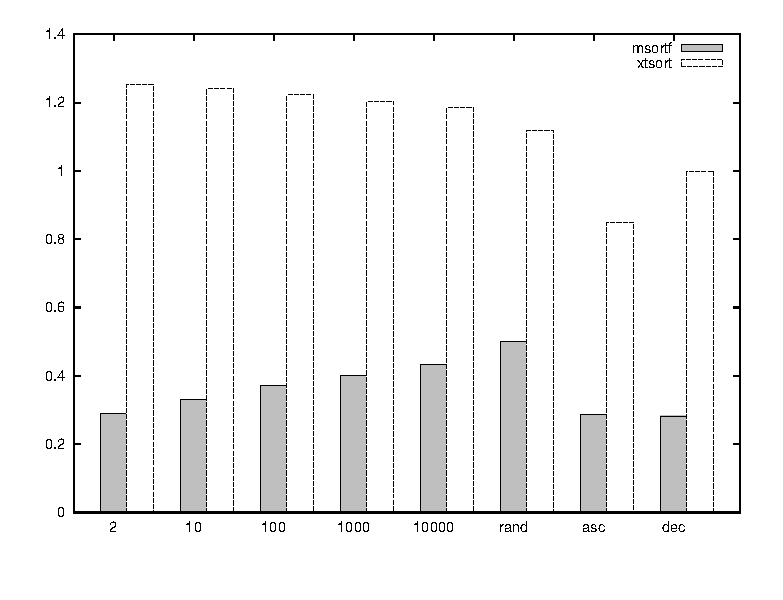
\includegraphics[scale=.8]{figure/msortf/key.eps}
\end{center}
\vspace{10 mm}
\caption{Compare sort results on character strings with msort, msortf, xtsort on various key types. (x-axis: number of the key types, y-axis: seconds)\label{fig:msortf:bench1}}
\end{figure}

%The graph of item (4) and (5) in the above table is shown below. 
\begin{figure}[hbt]
\begin{center}
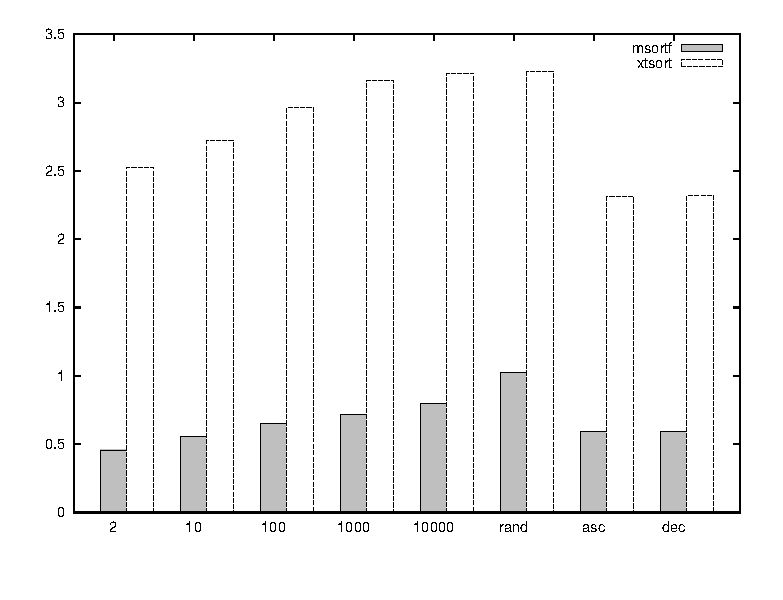
\includegraphics[scale=.8]{figure/msortf/num.eps}
\end{center}
\vspace{10 mm}
\caption{Compare sort results on numerical values with msortf,xtsort on various key types (x-axis: number of key types, y-axis: seconds)\label{fig:msortf:bench2}}
\end{figure}

msortf is 2 to 5 times faster than xtsort. In relation to sort, it can be more than ten times faster depending on the conditions. This command uses the exactly the same quick sort algorithm as in MUSASHI, however, in MCMD multi-threading is used for the parallel processing of sort in separate threads. The impact of the difference is shown. 

Next, the experiment shows the change in speed of character string sorting from 1 million records to 10 million records given the number of key types is set as 100 and the maximum value. 
The comparison of the two commands msortf and xtsort is shown in Figure \ref{fig:msortf:bench3}, \ref{fig:msortf:bench4}. 


%As shown in the benchmark test, msort is 1.5 times faster than MUSASHI xtsort. Even though both commands uses the same quicksort algorithm, msort leverages on multi-threaded sort processing using kgmod which runs 1.5 times faster. 
%msort performs better than msortf on data with irregular keys that is sorted beforehand, as sorting is done by line without dividing the data. Thus, small variation in key types for the first item makes it difficult for comparison as the correlation magnitude has not been established.  The need for comparison created a higher overhead. 
%In addition, the msort command process faster than msortf on data with multiple columns.  However, using msort to sort the key field of input data for other commands may yield different results if the command is executed incorrectly. For more information, refer to msort command. \\

%The results also show that msortf is two times more efficient than xtsort in sorting numeric fields.
%Next, the sorting speed is compared amongst msortf, msort, and xtsort on data with a sample size of 10 million with 2 to 100 different key values. The results are shown as follows: \\

\begin{figure}[hbt]
\begin{center}
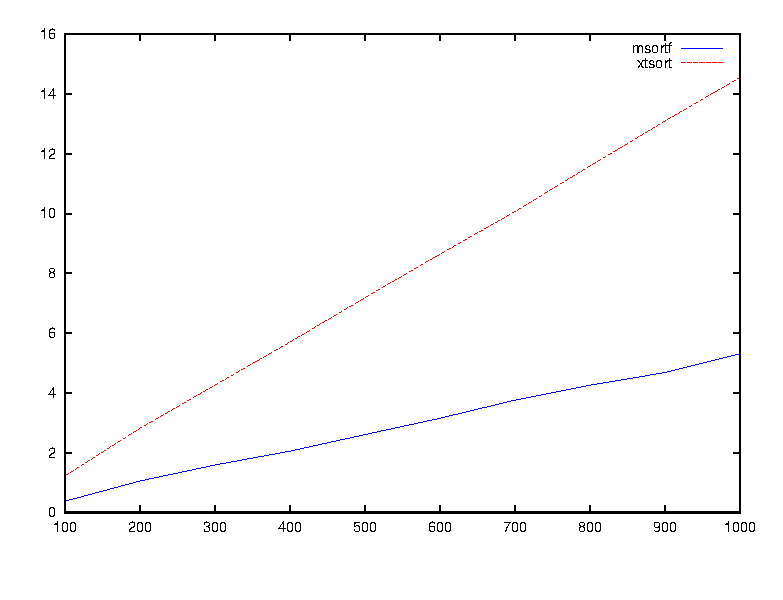
\includegraphics[scale=.8]{figure/msortf/line_100.eps}
\end{center}
\vspace{10 mm}
\caption{Sorting results with 100 key types (x-axis: number of records, y-axis: seconds)\label{fig:msortf:bench3}}
\end{figure}

\begin{figure}[hbt]
\begin{center}
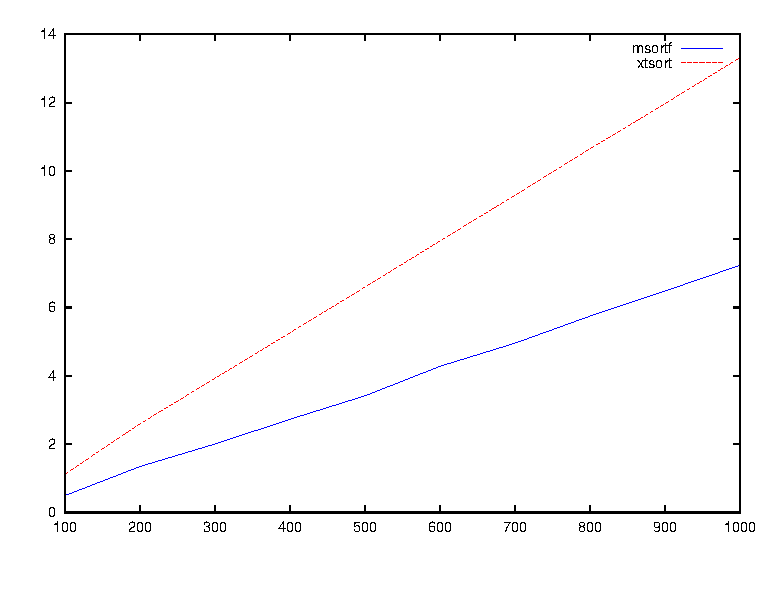
\includegraphics[scale=.8]{figure/msortf/line_rand.eps}
\end{center}
\vspace{10 mm}
\caption{Sorting results with different key types using random number (maximum) (x-axis: number of records, y-axis: seconds)\label{fig:msortf:bench4}}
\end{figure}

\subsection*{Related Command}


%\end{document}


%\begin{document}

\section{msplit 区切り文字による項目分割\label{sect:msplit}}
\index{msplit@msplit}
区切り文字によって項目を分割する。

\subsection*{書式}
\verb|msplit f= a= [-r] [delim=]|
\hyperref[sect:option_i]{[i=]}
\hyperref[sect:option_o]{[o=]}
\hyperref[sect:option_assert_diffSize]{[-assert\_diffSize]}
\hyperref[sect:option_assert_nullin]{[-assert\_nullin]}
\hyperref[sect:option_assert_nullout]{[-assert\_nullout]}
\hyperref[sect:option_nfn]{[-nfn]} 
\hyperref[sect:option_nfno]{[-nfno]}  
\hyperref[sect:option_x]{[-x]}
\hyperref[sect:option_option_tmppath]{[tmpPath=]}
\hyperref[sect:option_precision]{[precision=]}
\verb|[-params]|
\verb|[--help]|
\verb|[--helpl]|
\verb|[--version]|\\

\subsection*{パラメータ}
\begin{table}[htbp]
%\begin{center}
{\small
\begin{tabular}{ll}
\verb|i=|    & 入力ファイル名を指定する。\\
\verb|o=|    & 出力ファイル名を指定する。\\ 
\verb|f=|    & 区切り文字で分割するデータの項目名を指定する\\
\verb|a=|    & 新項目を指定する\\
             & ここで指定した項目名分分割される。足りない分はNULLとなる\\
\verb|delim=| & 新しい区切り文字を指定する。デフォルト値は半角スペース。\\
\verb|-r|    & \verb|f=|で指定した項目を取り除く\\
\end{tabular} 
}
\end{table} 

\subsection*{利用例}
\subsubsection*{例1: 基本例}

 半角スペースで分割


\begin{Verbatim}[baselinestretch=0.7,frame=single]
$ more dat1.csv
id,data
A,1 10 2
A,2 20 3
B,1 15 5
B,3 10 4
B,1 20 6
$ msplit f=data a=d1,d2,d3 i=dat1.csv o=rsl1.csv
#END# kgsplit a=d1,d2,d3 f=data i=dat1.csv o=rsl1.csv
$ more rsl1.csv
id,data,d1,d2,d3
A,1 10 2,1,10,2
A,2 20 3,2,20,3
B,1 15 5,1,15,5
B,3 10 4,3,10,4
B,1 20 6,1,20,6
\end{Verbatim}
\subsubsection*{例2: -r利用}

\verb|-r|を指定することで、\verb|f=|で項目を削除できる。


\begin{Verbatim}[baselinestretch=0.7,frame=single]
$ msplit f=data a=d1,d2,d3 -r i=dat1.csv o=rsl2.csv
#END# kgsplit -r a=d1,d2,d3 f=data i=dat1.csv o=rsl2.csv
$ more rsl2.csv
id,d1,d2,d3
A,1,10,2
A,2,20,3
B,1,15,5
B,3,10,4
B,1,20,6
\end{Verbatim}
\subsubsection*{例3: 分割数不一致}

\verb|a=|で指定した項目数よりも分割できる項目数が少ない場合は、NULLが追加され、
多い場合、先頭から指定した分割数まで出力する


\begin{Verbatim}[baselinestretch=0.7,frame=single]
$ more dat2.csv
id,data
A,1 10 2
A,2 20 3
B,1 15 5
B,3 4
B,1
$ msplit f=data a=d1,d2 i=dat2.csv o=rsl3.csv
#END# kgsplit a=d1,d2 f=data i=dat2.csv o=rsl3.csv
$ more rsl3.csv
id,data,d1,d2
A,1 10 2,1,10
A,2 20 3,2,20
B,1 15 5,1,15
B,3 4,3,4
B,1,1,
\end{Verbatim}
\subsubsection*{例4: delim指定}

\verb|delim=|を使用して半角スペース以外の文字で分割する


\begin{Verbatim}[baselinestretch=0.7,frame=single]
$ more dat3.csv
id,data
A,1_10_3
A,2_20_5
B,1_15_6
B,3_10_7
B,1_20_8
$ msplit f=data a=d1,d2,d3 delim=_ i=dat3.csv o=rsl4.csv
#END# kgsplit a=d1,d2,d3 delim=_ f=data i=dat3.csv o=rsl4.csv
$ more rsl4.csv
id,data,d1,d2,d3
A,1_10_3,1,10,3
A,2_20_5,2,20,5
B,1_15_6,1,15,6
B,3_10_7,3,10,7
B,1_20_8,1,20,8
\end{Verbatim}

\subsection*{関連コマンド}

%\end{document}


%\documentclass[a4paper]{book}
%\usepackage{mcmd}
%\begin{document}

\section{mstats - Calculate Statistics of 1 Variable\label{sect:mstats}}
\index{mstats@mstats}

Specify the numeric fields in the parameter \verb|f=|, and calculate the statistics specified in the parameter \verb|c=|. Specify the aggregate key unit at \verb|k=|. NULL value in the specified field(s) at \verb|f=| are ignored. However, if all records include NULL values, NULL values will be included in the output.


\subsection*{Format}
\verb|mstats c= f= [k=] [-n] | 
\hyperref[sect:option_i]{[i=]}
\hyperref[sect:option_o]{[o=]}
\hyperref[sect:option_assert_diffSize]{[-assert\_diffSize]}
\hyperref[sect:option_assert_nullkey]{[-assert\_nullkey]}
\hyperref[sect:option_assert_nullin]{[-assert\_nullin]}
\hyperref[sect:option_assert_nullout]{[-assert\_nullout]}
\hyperref[sect:option_nfn]{[-nfn]} 
\hyperref[sect:option_nfno]{[-nfno]}  
\hyperref[sect:option_x]{[-x]}
\hyperref[sect:option_q]{[-q]}
\hyperref[sect:option_option_tmppath]{[tmpPath=]}
\hyperref[sect:option_precision]{[precision=]}
\verb|[--help]|
\verb|[--helpl]|
\verb|[--version]|\\


\subsection*{Parameters}
\begin{table}[htbp]
%\begin{center}
{\small
\begin{tabular}{ll}
\verb|k=|    & Compute aggregate statistics on the key field(s) specified (multiple fields can be specified). \\

\verb|f=|    & Fields for which statistics are computed (multiple fields can be specified).\\
\verb|c=|    & Statistics (select one from the list below)\\
             & \verb/sum|mean|count|ucount|devsq|var|uvar|sd|usd|USD|cv|min|qtile1|/\\
             & \verb/median|qtile3|max|range|qrange|mode|skew|uskew|kurt|ukurt/\\
\verb|-n|    & Flag to be NULL if null data.\\
\end{tabular} 
}
\end{table} 

\subsection*{List of statistics}
\begin{table}[t]
%\begin{center}
{\small
\renewcommand{\arraystretch}{1.5}
\begin{tabular}{lp{4cm}lp{4cm}lp{3cm}l}
\hline
Value of \verb|c=| & Description & Equation & Remarks \\
\hline
count  & Count (Except NULL value) & $n$: Number of non-NULL records & It can not be applied to character string field.\\
ucount & Unique count     & $un$: Number of duplicate values removed &  It can not be applied to character string field. \\
sum    & Total             & $sum=\sum_{i=1}^n x_i$ & \\
mean   & Arithmetic mean         & $m=\frac{1}{n}\sum_{i=1}^n x_i$ & \\
devsq  & Sum of squared deviation       & $S=\sum_{i=1}^n(x_i-m)^2$ & \\
var    & Variance             & $s^2=\frac{1}{n}S$ & \\
uvar   & Variance (unbiased estimate) & $u^2=\frac{1}{n-1}S$ & \\
sd     & Standard deviation         & $s=\sqrt{s^2}$ & \\
usd    & Standard deviation (unbiased variance) & $u=\sqrt{u^2}$ & commonly used standard deviation\\
USD    & Unbiased standard deviation     & Omission              & Accurate unbiased estimation \\
cv     & Coefficient of variation  & $cv=s/mx100\%$ & \\
mode   & Mode           & $mode$: Most frequent value & Print the value of the smaller value if the frequency is same \\
       &                  &                   & Print NULL if values are different.\\
min    & Minimum value           & $min=\min_i x_i$ & \\
max    & Maximum value           & $max=\max_i x_i$ & \\
range  & Range             & $r=max-min$  & \\
median & Median           & $Q2=Second quartile when sorted in ascending order$ & \\
qtile1 & First quartile      & $Q1=First quartile when sorted in ascending order$ & \\
%qtile1 & 第1四分位点      & $Q1$ 第1四分位順位が自然数でない場合:$Q1=(\lceil t\rceil -t)x\lfloor t\rfloor +(t-\lfloor t \rfloor)x\lceil t\rceil$ただし,$t=1+0.25(n-1)$ & \\
qtile3 & Third quartile      & $Q3=Third quartile when sorted in ascending order$ & \\
% 第3四分位順位が自然数でない場合:$Q3=(\lceil t\rceil -t)x\lfloor t\rfloor +(t-\lfloor t \rfloor)x\lceil t\rceil$ただし,$t=1+0.75(n-1)$ \\
qrange & Interquartile range      & $rq=Q3-Q1$ & \\
skew   & Skewness             & $\frac{\frac{1}{n}\sum_{i=1}^n (x_i-m)^3}{s^3}$ & \\
uskew  & Skewness (unbiased estimate) & omitted & \\
kurt   & Kurtosis             & $\frac{\frac{1}{n}\sum_{i=1}^n (x_i-m)^4}{s^4}-3.0$ & \\
ukurt  & Kurtosis (unbiased estimated) & omitted & \\
\hline \\
\end{tabular}
}
\end{table}

\subsection*{Examples}
\subsubsection*{例1: 基本例}

「顧客」項目を単位に「数量」と「金額」項目の
各統計量合計値を計算する。


\begin{Verbatim}[baselinestretch=0.7,frame=single]
$ more dat1.csv
顧客,数量,金額
A,1,10
B,5,20
B,2,10
C,1,15
C,3,10
C,1,21
$ mstats k=顧客 f=数量,金額 c=sum i=dat1.csv o=rsl1.csv
#END# kgstats c=sum f=数量,金額 i=dat1.csv k=顧客 o=rsl1.csv
$ more rsl1.csv
顧客%0,数量,金額
A,1,10
B,7,30
C,5,46
\end{Verbatim}
\subsubsection*{例2: 基本例2}

各統計量最大値を計算する。


\begin{Verbatim}[baselinestretch=0.7,frame=single]
$ mstats k=顧客 f=数量,金額 c=max i=dat1.csv o=rsl2.csv
#END# kgstats c=max f=数量,金額 i=dat1.csv k=顧客 o=rsl2.csv
$ more rsl2.csv
顧客%0,数量,金額
A,1,10
B,5,20
C,3,21
\end{Verbatim}

\subsection*{Related Commands}
\hyperref[sect:msim]{msim} : Find out the bivariate statistics.

\hyperref[sect:mavg] {mavg} : Commands specific to\verb|c=avg|.

\hyperref[sect:msum] {msum} : Commands specific to \verb|c=sum|.

\hyperref[sect:mcount] {mcount} : Unlike \verb|c=count|, this count the number of rows for each aggregate key.

%\end{document}


%\begin{document}

\section{msum - Sum of Column\label{sect:msum}}
\index{msum@msum}

Aggregate the sum of values in the records at the specified field defined at \verb|f=| parameter for records with the same key value defined at \verb|k=|. \\

\subsection*{Format}
\verb|msum f= [k=] [-n]| 
\hyperref[sect:option_i]{[i=]}
\hyperref[sect:option_o]{[o=]}
\hyperref[sect:option_assert_diffSize]{[-assert\_diffSize]}
\hyperref[sect:option_assert_nullkey]{[-assert\_nullkey]}
\hyperref[sect:option_assert_nullin]{[-assert\_nullin]}
\hyperref[sect:option_assert_nullout]{[-assert\_nullout]}
\hyperref[sect:option_nfn]{[-nfn]} 
\hyperref[sect:option_nfno]{[-nfno]}  
\hyperref[sect:option_x]{[-x]}
\hyperref[sect:option_q]{[-q]}
\hyperref[sect:option_tmpPath]{[tmpPath=]} 
\hyperref[sect:option_precision]{[precision=]}
\verb|[--help]|
\verb|[--helpl]|
\verb|[--version]|\\

\subsection*{Parameters}
\begin{table}[htbp]
%\begin{center}
{\small
\begin{tabular}{ll}
\verb|k=|    & Specify list of field name(s) (multiple fields can be specified) as aggregate unit. \\

\verb|f=|    & Aggregate the values specified at the field(s) (multiple items can be specified). Records with NULL values are ignored. \\
\verb|-n|    & If NULL exist in the field defined at \verb|f=|, the result will return NULL. \\
\end{tabular} 
}
\end{table} 

\subsection*{Examples}
\subsubsection*{Example 1: Basic Example}

Calculate the total value of "quantity" and "amount" for each "customer".  Save the output with field names "total quantity" and "total amount".


\begin{Verbatim}[baselinestretch=0.7,frame=single]
$ more dat1.csv
customer,quantity,amount
A,1,10
A,2,20
B,1,15
B,3,10
B,1,20
$ msum k=customer f=quantity:quantitySum,amount:amountSum i=dat1.csv o=rsl1.csv
#END# kgsum f=quantity:quantitySum,amount:amountSum i=dat1.csv k=customer o=rsl1.csv
$ more rsl1.csv
customer%0,quantitySum,amountSum
A,3,30
B,5,45
\end{Verbatim}

\subsection*{Related Commands}
\hyperref[sect:mhashsum]{mhashsum} : Compute sum without sorting by aggregate key in advance. 

\hyperref[sect:mavg]{mavg} : Compute average. 

\hyperref[sect:mstats]{mstats} : Compute a variety of statistics.

%\end{document}


%\begin{document}

\section{msummary Calculate Statistics for 1 Variable \label{sect:msummary}}
\index{msummary@msummary}
Calculate the type of statistics specified at \verb|c=| parameter for fields specified at  \verb|f=| parameter. \\

\subsection*{Format}
\verb|msummary c= f= [a=] [k=] [-n] | 
\hyperref[sect:option_i]{[i=]}
\hyperref[sect:option_o]{[o=]}
\hyperref[sect:option_assert_diffSize]{[-assert\_diffSize]}
\hyperref[sect:option_assert_nullkey]{[-assert\_nullkey]}
\hyperref[sect:option_assert_nullin]{[-assert\_nullin]}
\hyperref[sect:option_assert_nullout]{[-assert\_nullout]}
\hyperref[sect:option_nfn]{[-nfn]} 
\hyperref[sect:option_nfno]{[-nfno]}  
\hyperref[sect:option_x]{[-x]}
\hyperref[sect:option_q]{[-q]}
\hyperref[sect:option_option_tmppath]{[tmpPath=]}
\hyperref[sect:option_precision]{[precision=]}
\verb|[--help]|
\verb|[--helpl]|
\verb|[--version]|\\

\subsection*{Parameters}
\begin{table}[htbp]
%\begin{center}
{\small
\begin{tabular}{ll}
\verb|k=|    & Compute statistics based on the key field(s) specified (multiple fields can be specified). \\


\verb|f=|    & Field lists for computation of statistical summary (multiple fields can be specified). \\

			 & When \verb|-x|,\verb|-nfn| option is specified, specify the field number  (0~). \\
\verb|c=|    & Statistics (multiple fields can be specified) \\
             & Specify list of statistics delimited by comma. \\
			 & Statistics list: \\
			 & \verb|sum/mean/count/ucount/devsq/var/uvar/sd/usd/cv/min/qtile1/median/qtile3/max/| \\
			 & \verb|range/qrange/mode/skew/uskew/kurt/ukurt| \\
\verb|-a|    & New column name. \\
             & Results from calculation on column(s) specified at \verb|f=| parameter (default is fld).  \\
\end{tabular} 
}
\end{table} 

\subsection*{List of Statistics }

The list of statistics specified at \verb|c=| parameter is shown in Table \ref{tbl:msummary}. 

\begin{table}[t]
%\begin{center}
\caption{List of Statistics \label{tbl:msummary}}
{\small
\renewcommand{\arraystretch}{1.5}
\begin{tabular}{lp{4cm}lp{4cm}lp{3cm}l}
\hline
Value of \verb|c=| & Description & Equation & Remarks \\  
\hline
count  & Count (Except NULL value) & $n$: Number of non-NULL records & It can not be applied to character string field.\\
ucount & Unique count     & $un$: Number of duplicate values removed &  It can not be applied to character string field. \\
sum    & Total             & $sum=\sum_{i=1}^n x_i$ & \\
mean   & Arithmetic mean           & $m=\frac{1}{n}\sum_{i=1}^n x_i$ & \\
devsq  & Sum of squared deviation       & $S=\sum_{i=1}^n(x_i-m)^2$ & \\
var    & Variance             & $s^2=\frac{1}{n}S$ & \\
uvar   & Variance (unbiased estimate) & $u^2=\frac{1}{n-1}S$ & \\
sd     & Standard deviation         & $s=\sqrt{s^2}$ & \\
usd    & Standard deviation (sort of unbiased variance) & $u=\sqrt{u^2}$ & commonly used standard deviation \\  
cv     & Coefficient of variation       & $cv=s/m100\%$ & \\
mode   & Mode           & $mode$: Most frequent value & Print the value of the smaller value\\
       &                  &                   & if the frequency is same. \\
min    & Minimum value            & $min=\min_i x_i$ & \\
max    & Maximum value          & $max=\max_i x_i$ & \\
range  & Range            & $r=max-min$  & \\
median & Median           & $Q2=Second quartile when sorted in ascending order$ & \\
qtile1 & First quartile      & $Q1=First quartile when sorted in ascending order$ & \\
%qtile1 & 第1四分位点      & $Q1$ 第1四分位順位が自然数でない場合:$Q1=(\lceil t\rceil -t)x\lfloor t\rfloor +(t-\lfloor t \rfloor)x\lceil t\rceil$ただし,$t=1+0.25(n-1)$ & \\
qtile3 & Third quartile      & $Q3=Third quartile when sorted in ascending order$ & \\
% 第3四分位順位が自然数でない場合:$Q3=(\lceil t\rceil -t)x\lfloor t\rfloor +(t-\lfloor t \rfloor)x\lceil t\rceil$ただし,$t=1+0.75(n-1)$ \\
qrange & Interquartile range       & $rq=Q3-Q1$ & \\
skew   & Skewness             & $\frac{\frac{1}{n}\sum_{i=1}^n (x_i-m)^3}{s^3}$ & \\
uskew  & Skewness (unbiased estimate) & omitted & \\
kurt   & Kurtosis             & $\frac{\frac{1}{n}\sum_{i=1}^n (x_i-m)^4}{s^4}-3.0$ & \\
ukurt  & Kurtosis (unbiased estimate) & omitted & \\
\hline \\
\end{tabular}
}
\end{table}


\subsection*{Examples}
\subsubsection*{例1: 基本例}

「顧客」項目を単位に「数量」と「金額」項目の中央値・平均値を求める。
統計量を求めた項目名は「変数」という項目に出力する。


\begin{Verbatim}[baselinestretch=0.7,frame=single]
$ more dat1.csv
顧客,数量,金額
A,1,10
A,2,20
B,1,15
B,3,10
B,1,20
$ msummary k=顧客 f=数量,金額 c=median:中央値,mean:平均値 a=変数 i=dat1.csv o=rsl1.csv
#END# kgsummary a=変数 c=median:中央値,mean:平均値 f=数量,金額 i=dat1.csv k=顧客 o=rsl1.csv
$ more rsl1.csv
顧客%0,変数,中央値,平均値
A,数量,1.5,1.5
A,金額,15,15
B,数量,1,1.666666667
B,金額,15,15
\end{Verbatim}

\subsection*{Related Commands}
\hyperref[sect:mstats]{mstats} : Compute one type of statistics. 

%\end{document}


%\documentclass[a4paper]{jsbook}
%\usepackage{mcmd_jp}
%\begin{document}

\section{mtab2csv TSVからCSVデータへの変換\label{sect:mtab2csv}}
\index{mtab2csv@mtab2csv}
タブ区切りデータをCSVデータへ変換する。
\verb|d=|で区切り文字を指定することで、タブ以外の区切り文字のテキストファイルも
変換することが可能である。 
変換後の項目数に違いある場合には、その直前行まで出力され、
その後エラー終了する。


\subsection*{書式}
\verb|mtab2csv [d=] [-r] |
\hyperref[sect:option_i]{[i=]}
\hyperref[sect:option_o]{[o=]}
\hyperref[sect:option_assert_diffSize]{[-assert\_diffSize]}
\hyperref[sect:option_nfn]{[-nfn]} 
\hyperref[sect:option_nfno]{[-nfno]}  
\hyperref[sect:option_x]{[-x]}
\hyperref[sect:option_option_tmppath]{[tmpPath=]}
\hyperref[sect:option_precision]{[precision=]}
\verb|[-params]|
\verb|[--help]|
\verb|[--helpl]|
\verb|[--version]|\\

\subsection*{パラメータ}
\begin{table}[htbp]
%\begin{center}
{\small
\begin{tabular}{ll}
\verb|i=|    & 入力ファイル名を指定する。\\
\verb|o=|    & 出力ファイル名を指定する。\\
\verb|d=|    & 区切り文字の指定(1バイト文字のみ指定可)。\\
\verb|-r|    & 改行コード(CR:\verb|\r|)を取り除く。\\
             & MCMDが扱うCSVは改行コードがLF(\verb|\n|)固定であるため、\\
             & Windowsのテキスト改行CR+LF(\verb|\r\n|)やMacのテキスト改行CR(\verb|\r|)があれば、\\
             & 単なる文字列として扱ってしまい、変換後に不具合が生じる。\\
             & この問題を回避するためのオプションである。\\
\end{tabular} 
}
\end{table} 

\subsection*{利用例}
\subsubsection*{Example 1: Example 1: Basic example}

TSV data is converted into CSV data.


\begin{Verbatim}[baselinestretch=0.7,frame=single]
$ more dat1.tab
id	data	data2
A	1102	a
A	2203	aaa
B	1155	bbbb
B	3104	c
B	1206	de
$ mtab2csv i=dat1.tab o=rsl1.csv
#END# kgtab2csv i=dat1.tab o=rsl1.csv
$ more rsl1.csv
id,data,data2
A,1102,a
A,2203,aaa
B,1155,bbbb
B,3104,c
B,1206,de
\end{Verbatim}
\subsubsection*{Example 2: Example 2: Specifying d=}

The \verb|d=| parameter is specified to use a delimiter other than the tab.


\begin{Verbatim}[baselinestretch=0.7,frame=single]
$ more dat2.bar
id-data-data2
A-1102-a
A-2203-aaa
B-1155-bbbb
B-3104-c
B-1206-de
$ mtab2csv d=- i=dat2.bar o=rsl2.csv
#END# kgtab2csv d=- i=dat2.bar o=rsl2.csv
$ more rsl2.csv
id,data,data2
A,1102,a
A,2203,aaa
B,1155,bbbb
B,3104,c
B,1206,de
\end{Verbatim}

\subsection*{関連コマンド}
\hyperref[sect:mxml2csv]{mxml2csv}:XMLデータをCSVデータへ変換する

\hyperref[sect:msplit]{msplit}:項目値の区切り文字によるデータ分割
%\end{document}


%\documentclass[a4paper]{jsbook}
%\usepackage{mcmd_jp}
%\begin{document}

\section{mtee 複数ファイルへのコピー\label{sect:mtee}}
入力データの内容を標準出力および複数ファイルへそのままコピー出力する。

\subsection*{書式}
\verb|mtee [o=] [-nostdout]|
[\hyperref[sect:option_i]{i=}] 
[\hyperref[sect:option_nfn]{-nfn}] 
[\hyperref[sect:option_nfno]{-nfno}]  
[\hyperref[sect:option_x]{-x}] 
\hyperref[sect:option_option_tmppath]{[tmpPath=]}
\hyperref[sect:option_precision]{[precision=]}
\verb|[-params]|
\verb|[--help]|
\verb|[--helpl]|
\verb|[--version]|\\

\subsection*{パラメータ}
\begin{table}[htbp]
%\begin{center}
{\small
\begin{tabular}{ll}
\verb|i=|        & 入力ファイル名を指定する。\\
\verb|o=|        & ここで指定された複数のファイルに入力ファイルと同一内容が出力される。\\
                 & またこのパラメータが省略された時には標準出力にのみ出力される。\\
\verb|-nostdout| & 標準出力には出力しない場合に指定する。\\
\end{tabular} 
}
\end{table} 

\subsection*{利用例}
\subsubsection*{Example 1: Basic Examples}

Copy \verb|dat1.csv| file to two files \verb|rsl1.csv| and \verb|rsl2.csv| In addition, display output on screen through standard output.


\begin{Verbatim}[baselinestretch=0.7,frame=single]
$ more dat1.csv
customer,quantity,price
A,1,10
A,2,20
B,1,15
$ mtee i=dat1.csv o=rsl1.csv,rsl2.csv
customer,quantity,price
A,1,10
A,2,20
B,1,15
#END# kgtee i=dat1.csv o=rsl1.csv,rsl2.csv
$ more rsl1.csv
customer,quantity,price
A,1,10
A,2,20
B,1,15
$ more rsl2.csv
customer,quantity,price
A,1,10
A,2,20
B,1,15
\end{Verbatim}
\subsubsection*{Example 2: Do not print to standard output }

When \verb|-nostdout| is specified, the command only copy the two files \verb|rsl1.csv| and \verb|rsl2.csv| but not to standard output.


\begin{Verbatim}[baselinestretch=0.7,frame=single]
$ mtee i=dat1.csv o=rsl1.csv,rsl2,csv -nostdout
#END# kgtee -nostdout i=dat1.csv o=rsl1.csv,rsl2,csv
\end{Verbatim}


\subsection*{関連コマンド}

%\end{document}


%\begin{document}

\section{mtonull - Substitute Value for NULL\label{sect:mtonull}}
\index{mtonull@mtonull}
Specify the target field parameter at \verb|f=| , substitute the value at the \verb|v=| parameter with NULL in the data. Select the methods for finding patterns using exact string matching (the default) or substring matching (\verb|-sub| option). 


\subsection*{Format}
\verb|mtonull f= v= [-sub] [-W]|
\hyperref[sect:option_i]{[i=]}
\hyperref[sect:option_o]{[o=]}
\hyperref[sect:option_assert_diffSize]{[-assert\_diffSize]}
\hyperref[sect:option_assert_nullin]{[-assert\_nullin]}
\hyperref[sect:option_nfn]{[-nfn]} 
\hyperref[sect:option_nfno]{[-nfno]}  
\hyperref[sect:option_x]{[-x]}
\hyperref[sect:option_q]{[-q]}
\hyperref[sect:option_option_tmppath]{[tmpPath=]}
\verb|[--help]|
\verb|[--helpl]|
\verb|[--version]|\\

\subsection*{Parameters}
\begin{table}[htbp]
%\begin{center}
{\small
\begin{tabular}{ll}
\verb|f=|  & specify list of field name(s) (multiple fields can be specified) where the values are replaced .\\
\verb|v=|  & Specify the character string value (multiple items can be specified) for matching the field defined at \verb|f=| parameter. \\
           & Replace the matched values with NULL.\\
\end{tabular} 
}
\end{table} 

\subsection*{Options}
\begin{table}[htbp]
%\begin{center}
{\small
\begin{tabular}{ll}
\verb|-sub|    & Rather than matching the exact string, \\
		& compare character substring with the values in the field specified in the \verb|f=| parameter \\
		& and replace the value defined in the \verb|v=| parameter containing the substring with NULL value.\\
\verb|-W|      & Substring match for wide character strings when the \verb|-sub| option is specified. \\
\end{tabular} 
}
\end{table} 

\subsection*{Examples}
\subsubsection*{Example 1: Basic Example}

Replace 0 with NULL value in columns \verb|quantity| and \verb|price|.


\begin{Verbatim}[baselinestretch=0.7,frame=single]
$ more dat1.csv
item,quantity,price
A,0,1
B,1,0
C,2,200
D,3,0
E,0,298
$ mtonull f=quantity,price v=0 i=dat1.csv o=rsl1.csv
#END# kgtonull f=quantity,price i=dat1.csv o=rsl1.csv v=0
$ more rsl1.csv
item,quantity,price
A,,1
B,1,
C,2,200
D,3,
E,,298
\end{Verbatim}
\subsubsection*{Example 2: Replace a specified number with NULL value}

Replace 0 or 1 with NULL value in columns \verb|quantity| and \verb|price|.


\begin{Verbatim}[baselinestretch=0.7,frame=single]
$ mtonull f=quantity,price v=0,1 i=dat1.csv o=rsl2.csv
#END# kgtonull f=quantity,price i=dat1.csv o=rsl2.csv v=0,1
$ more rsl2.csv
item,quantity,price
A,,
B,,
C,2,200
D,3,
E,,298
\end{Verbatim}
\subsubsection*{Example 3: Substitute substring match}

Replace with a NULL value where \verb|quantity| and \verb|price| columns contain 0.


\begin{Verbatim}[baselinestretch=0.7,frame=single]
$ mtonull -sub f=quantity,price v=0 i=dat1.csv o=rsl3.csv
#END# kgtonull -sub f=quantity,price i=dat1.csv o=rsl3.csv v=0
$ more rsl3.csv
item,quantity,price
A,,1
B,1,
C,2,
D,3,
E,,298
\end{Verbatim}
\subsubsection*{Example 4: Substitute character string}

Replace the string in the \verb|item| field that matches character string \verb|apple, orange, pineapple| with NULL value.


\begin{Verbatim}[baselinestretch=0.7,frame=single]
$ more dat2.csv
item,price
fruit:apple,100
fruit:peach,250
fruit:grape,300
fruit:pineapple,450
fruit:orange,500
$ mtonull f=item v=apple,orange,pineapple -sub i=dat2.csv o=rsl4.csv
#END# kgtonull -sub f=item i=dat2.csv o=rsl4.csv v=apple,orange,pineapple
$ more rsl4.csv
item,price
,100
fruit:peach,250
fruit:grape,300
,450
,500
\end{Verbatim}

\subsection*{Related Command}
\hyperref[sect:mnullto]{mnullto} : Reversely, replace NULL value with a character string.

%\end{document}


%\begin{document}

\section{mtra - Convert Vertical Data to Vector\label{sect:mtra}}
\index{mtra@mtra}
Connect the items from the specified fields in \verb|f=|,  and save the string of items as a vector in a new column (referred to as transaction field). 
Specify the delimiter character of the items at \verb|delim=|.


\subsection*{Format}
\verb|mtra f= [s=] [k=] [delim=] [-r]  | 
\hyperref[sect:option_i]{[i=]}
\hyperref[sect:option_o]{[o=]}
\hyperref[sect:option_assert_diffSize]{[-assert\_diffSize]}
\hyperref[sect:option_assert_nullkey]{[-assert\_nullkey]}
\hyperref[sect:option_assert_nullin]{[-assert\_nullin]}
\hyperref[sect:option_assert_nullout]{[-assert\_nullout]}
\hyperref[sect:option_nfn]{[-nfn]} 
\hyperref[sect:option_nfno]{[-nfno]}  
\hyperref[sect:option_x]{[-x]}
\hyperref[sect:option_q]{[-q]}
\hyperref[sect:option_option_tmppath]{[tmpPath=]}
\verb|[--help]|
\verb|[--helpl]|
\verb|[--version]|\\

\subsection*{Parameters}
\begin{table}[htbp]
%\begin{center}
{\small
\begin{tabular}{ll}
\verb|f=|        & Specify field(s) (multiple fields can be specified) where the transaction fields are connected as an item.\\
                 & NULL values will not be included in the vector.\\
\verb|k=|        &  Key field name(s) (multiple items can be specified) of the character string pattern. \\
                 & \verb|-r| option cannot be specified with this parameter. \\
\verb|delim=|    & Specify the delimiting character (Space is used as the default delimiter).\\
\verb|-r|        & Reverse conversion\\
                 & Convert transaction items column to vertically structured data.\\
\end{tabular} 
}
\end{table} 

\subsection*{Examples}
\subsubsection*{Example 1: Basic Example}

Combine the corresponding \verb|item| for each \verb|customer| in a string using a space as the delimiter, and save output in the column named \verb|transaction|.


\begin{Verbatim}[baselinestretch=0.7,frame=single]
$ more dat1.csv
customer,item
A,a
A,b
B,c
B,d
B,e
$ mtra k=customer f=item:transaction i=dat1.csv o=rsl1.csv
#END# kgtra f=item:transaction i=dat1.csv k=customer o=rsl1.csv
$ more rsl1.csv
customer%0,transaction
A,a b
B,c d e
\end{Verbatim}
\subsubsection*{Example 2: Use hyphen (-) as item delimiter}



\begin{Verbatim}[baselinestretch=0.7,frame=single]
$ mtra k=customer f=item:transaction delim=- i=dat1.csv o=rsl2.csv
#END# kgtra delim=- f=item:transaction i=dat1.csv k=customer o=rsl2.csv
$ more rsl2.csv
customer%0,transaction
A,a-b
B,c-d-e
\end{Verbatim}
\subsubsection*{Example 3: Convert items in descending sort order}



\begin{Verbatim}[baselinestretch=0.7,frame=single]
$ mtra k=customer s=item%r f=item:transaction i=dat1.csv o=rsl3.csv
#END# kgtra f=item:transaction i=dat1.csv k=customer o=rsl3.csv s=item%r
$ more rsl3.csv
customer%0,transaction
A,b a
B,e d c
\end{Verbatim}

\subsection*{Related Commands}
\hyperref[sect:mvsort]{mvsort} : Vector based transaction data can be processed by a set of commands  (with \verb|mv| as prefix) which handles vector data. 

\hyperref[sect:mcross]{mcross} : Rather than converting as transaction data, every item is saved separately as individual field in the output. 

\hyperref[sect:mtrafld]{mtrafld} :  Create transaction data using “field name=value”.

\hyperref[sect:mtraflg]{mtraflg} : Create transaction data as item with field names.

%\end{document}


%\begin{document}

\section{mtrafld - Convert Transaction Field to Cross (pivot) Table\label{sect:mtrafld}}
\index{mtrafld@mtrafld}
Create item pairs from the fields specified at \verb|f=|, concatenate the item pairs and save as a new vector field (also referred to as transaction field).


\subsection*{Format}
\verb|mtrafld a= [f=] [delim=] [delim2=] [-r] [-valOnly] |   
\hyperref[sect:option_i]{[i=]}
\hyperref[sect:option_o]{[o=]}
\hyperref[sect:option_assert_diffSize]{[-assert\_diffSize]}
\hyperref[sect:option_assert_nullin]{[-assert\_nullin]}
\hyperref[sect:option_assert_nullout]{[-assert\_nullout]}
\hyperref[sect:option_nfn]{[-nfn]} 
\hyperref[sect:option_nfno]{[-nfno]}  
\hyperref[sect:option_x]{[-x]}
\hyperref[sect:option_q]{[-q]}
\hyperref[sect:option_option_tmppath]{[tmpPath=]}
\verb|[--help]|
\verb|[--helpl]|
\verb|[--version]|\\

\subsection*{Parameters}
\begin{table}[htbp]
%\begin{center}
{\small
\begin{tabular}{ll}
\verb|a=|      & Specify the transaction field name.\\
\verb|f=|      & List of field name(s) (Multiple fields can be specified) [required when \verb|-r| is specified, \\
		&  otherwise, this parameter is optional]\\
               & The field names specified here will be created as connected items and saved in the transaction field.\\
               & When -r option is specified, specify the field name to extract from the transaction data.\\
               & This parameter is optional when \verb|-r| option is specified.\\
               & If the parameter is not specified, all field names are processed as value pairs. \\
               & However, when\verb|f=| is not defined, this command cannot read standard input (using pipe). \\
\verb|delim=|  & Specify the character to separate each transaction field item (default delimiter: \\
		& space if this parameter is not defined).\\
\verb|delim2=| & Specify the character to separate value pairs and field name (default character: =).\\
\verb|-r|      & Reverse conversion\\
               & Convert transaction field to cross table. \\
\verb|-valOnly|& When this option is specified, the item do not return the prefix "field name=" in the output. \\
\end{tabular} 
}
\end{table} 

\subsection*{Examples}
\subsubsection*{Example 1: Basic Example}

Join the fields \verb|price| and \verb|quantity| to a string, rename output field as \verb|transaction|.



\begin{Verbatim}[baselinestretch=0.7,frame=single]
$ more dat1.csv
customer,price,quantity
A,198,1
B,325,2
C,200,3
D,450,2
E,100,1
$ mtrafld a=transaction f=price,quantity i=dat1.csv o=rsl1.csv
#END# kgtrafld a=transaction f=price,quantity i=dat1.csv o=rsl1.csv
$ more rsl1.csv
customer,transaction
A,price=198 quantity=1
B,price=325 quantity=2
C,price=200 quantity=3
D,price=450 quantity=2
E,price=100 quantity=1
\end{Verbatim}
\subsubsection*{Example 2: Basic Example 2}

Use \verb|-r| option to revert the output results back to the original data.


\begin{Verbatim}[baselinestretch=0.7,frame=single]
$ mtrafld -r a=transaction f=price,quantity i=rsl1.csv o=rsl2.csv
#END# kgtrafld -r a=transaction f=price,quantity i=rsl1.csv o=rsl2.csv
$ more rsl2.csv
customer,price,quantity
A,198,1
B,325,2
C,200,3
D,450,2
E,100,1
\end{Verbatim}
\subsubsection*{Example 3: Specify the delimiter}

\verb|Price| and \verb|quantity| field is separated by “\_” (underscore) character and connected by 1 character string. Use colon and name the output field as \verb|transaction|.


\begin{Verbatim}[baselinestretch=0.7,frame=single]
$ mtrafld a=transaction f=price,quantity delim=_ delim2=':' i=dat1.csv o=rsl3.csv
#END# kgtrafld a=transaction delim2=: delim=_ f=price,quantity i=dat1.csv o=rsl3.csv
$ more rsl3.csv
customer,transaction
A,price:198_quantity:1
B,price:325_quantity:2
C,price:200_quantity:3
D,price:450_quantity:2
E,price:100_quantity:1
\end{Verbatim}
\subsubsection*{Example 4: When data contains NULL value}



\begin{Verbatim}[baselinestretch=0.7,frame=single]
$ more dat2.csv
customer,price,quantity
A,198,1
B,,2
C,200,
D,450,2
E,,
$ mtrafld a=transaction f=price,quantity i=dat2.csv o=rsl4.csv
#END# kgtrafld a=transaction f=price,quantity i=dat2.csv o=rsl4.csv
$ more rsl4.csv
customer,transaction
A,price=198 quantity=1
B,quantity=2
C,price=200
D,price=450 quantity=2
E,
\end{Verbatim}
\subsubsection*{Example 5: When data contains NULL value 2}

Use \verb|-r| option to revert the output results back to the original data.


\begin{Verbatim}[baselinestretch=0.7,frame=single]
$ mtrafld -r a=transaction f=price,quantity i=rsl4.csv o=rsl5.csv
#END# kgtrafld -r a=transaction f=price,quantity i=rsl4.csv o=rsl5.csv
$ more rsl5.csv
customer,price,quantity
A,198,1
B,,2
C,200,
D,450,2
E,,
\end{Verbatim}
\subsubsection*{Example 6: Specify -valOnly option}



\begin{Verbatim}[baselinestretch=0.7,frame=single]
$ mtrafld -valOnly f=price,quantity a=transaction i=dat2.csv o=rsl6.csv
#END# kgtrafld -valOnly a=transaction f=price,quantity i=dat2.csv o=rsl6.csv
$ more rsl6.csv
customer,transaction
A,198 1
B,2
C,200
D,450 2
E,
\end{Verbatim}

\subsection*{Related Commands}
\hyperref[sect:mvsort] {mvsort} : Vector based transaction data can be processed by a set of commands  (with mv as prefix) which handles vector data.

\hyperref[sect:mcross] {mcross} : Rather than converting as transaction data, every item is saved separately as individual field in the output. 

\hyperref[sect:mtra] {mtra} : Create transaction data using values in the field.

\hyperref[sect:mtraflg] {mtraflg} :  Create transaction data with field names.

%\end{document}

%\documentclass[a4paper]{book}
%\usepackage{mcmd}
%\begin{document}
\section{mtraflg - Convert Cross (pivot) Table to Transaction Fields\label{sect:mtraflg}}
\index{mtraflg@mtraflg}
Check whether the field(s) specified in the f= parameter contains NULL value. Fields with non-NULL values are connected as one item and saved as a new vector. \\

\subsection*{Format}
\verb|mtraflg a= f= [delim=] [-r] | 
\hyperref[sect:option_i]{[i=]}
\hyperref[sect:option_o]{[o=]}
\hyperref[sect:option_assert_diffSize]{[-assert\_diffSize]}
\hyperref[sect:option_assert_nullin]{[-assert\_nullin]}
\hyperref[sect:option_assert_nullout]{[-assert\_nullout]}
\hyperref[sect:option_nfn]{[-nfn]} 
\hyperref[sect:option_nfno]{[-nfno]}  
\hyperref[sect:option_x]{[-x]}
\hyperref[sect:option_q]{[-q]}
\hyperref[sect:option_option_tmppath]{[tmpPath=]}
\verb|[--help]|
\verb|[--helpl]|
\verb|[--version]|\\

\subsection*{Parameters}
\begin{table}[htbp]
%\begin{center}
{\small
\begin{tabular}{ll}
\verb|a=|      & Specify the transaction field name.\\
\verb|f=|      & Check the values in the specified field name(s) (multiple fields can be specified)  to create transaction data.\\
               & (\verb|-r| option is specified, extract list of values as the field name of the transaction data)\\
\verb|delim=|  & Specify the character to separate each transaction field item (Default character is space if this parameter is omitted).\\
               & Character string should not be used. 1 byte character can be specified. \\
\verb|-r|      & Reverse conversion\\
               & Convert transaction based data to vertically structured data. \\
\end{tabular} 
}
\end{table} 

\subsection*{Examples}
\subsubsection*{Example 1: Basic Example}

Create a string of vector from the list of non-null values in column \verb|egg| and \verb|milk|.


\begin{Verbatim}[baselinestretch=0.7,frame=single]
$ more dat1.csv
customer,egg,milk
A,1,1
B,,1
C,1,
D,1,1
$ mtraflg f=egg,milk a=transaction i=dat1.csv o=rsl1.csv
#END# kgtraflg a=transaction f=egg,milk i=dat1.csv o=rsl1.csv
$ more rsl1.csv
customer,transaction
A,egg milk
B,milk
C,egg
D,egg milk
\end{Verbatim}
\subsubsection*{Example 2: Basic Example 2}

Use \verb|-r| option to revert the output results back to the original data.


\begin{Verbatim}[baselinestretch=0.7,frame=single]
$ mtraflg -r f=egg,milk a=transaction i=rsl1.csv o=rsl2.csv
#END# kgtraflg -r a=transaction f=egg,milk i=rsl1.csv o=rsl2.csv
$ more rsl2.csv
customer,egg,milk
A,1,1
B,,1
C,1,
D,1,1
\end{Verbatim}
\subsubsection*{Example 3: Specify the delimiter}

Combine items using the “-” (hyphen) as delimiter. Save output in column named \verb|transaction|.


\begin{Verbatim}[baselinestretch=0.7,frame=single]
$ mtraflg f=egg,milk a=transaction delim=- i=dat1.csv o=rsl3.csv
#END# kgtraflg a=transaction delim=- f=egg,milk i=dat1.csv o=rsl3.csv
$ more rsl3.csv
customer,transaction
A,egg-milk
B,milk
C,egg
D,egg-milk
\end{Verbatim}

\subsection*{Related Commands}
\hyperref[sect:mvsort] {mvsort} : Vector based transaction data can be processed by a set of commands  (with \verb|mv| as prefix) which handles vector data.

\hyperref[sect:mcross] {mcross} : Rather than converting as transaction data, every item is saved separately as individual field in the output.

\hyperref[sect:mtra] {mtra} : Create transaction data using values in the field.

\hyperref[sect:mtrafld] {mtrafld} :  Create transaction data with the format “field name=value”.
%\end{document}


%\begin{document}

\section{muniq - Unique Records\label{sect:muniq}}
\index{muniq@muniq}
Remove duplicate values and create unique records. 

\subsection*{Format}
\verb|muniq [k=] |
\hyperref[sect:option_i]{[i=]}
\hyperref[sect:option_o]{[o=]}
\hyperref[sect:option_assert_diffSize]{[-assert\_diffSize]}
\hyperref[sect:option_assert_nullkey]{[-assert\_nullkey]}
\hyperref[sect:option_nfn]{[-nfn]} 
\hyperref[sect:option_nfno]{[-nfno]}  
\hyperref[sect:option_x]{[-x]}
\hyperref[sect:option_q]{[-q]}
\hyperref[sect:option_option_tmppath]{[tmpPath=]}
\verb|[--help]|
\verb|[--helpl]|
\verb|[--version]|\\

\subsection*{Parameter}
\begin{table}[htbp]
%\begin{center}
{\small
\begin{tabular}{ll}
\verb|k=|    &  Specify the field name (s) as the unique identifier of the records. \\
\end{tabular} 
}
\end{table} 

\subsection*{Examples}
\subsubsection*{Example 1: Basic Example}

Remove duplicate records in the \verb|date| field.


\begin{Verbatim}[baselinestretch=0.7,frame=single]
$ more dat1.csv
date,customer
20081201,A
20081202,A
20081202,B
20081202,B
20081203,C
$ muniq k=date i=dat1.csv o=rsl1.csv
#END# kguniq i=dat1.csv k=date o=rsl1.csv
$ more rsl1.csv
date%0,customer
20081201,A
20081202,B
20081203,C
\end{Verbatim}
\subsubsection*{Example 2: Delete duplicate rows in multiple columns}

Remove duplicate records based on unique values in \verb|date| and \verb|customer| field.


\begin{Verbatim}[baselinestretch=0.7,frame=single]
$ muniq k=date,customer i=dat1.csv o=rsl2.csv
#END# kguniq i=dat1.csv k=date,customer o=rsl2.csv
$ more rsl2.csv
date%0,customer%1
20081201,A
20081202,A
20081202,B
20081203,C
\end{Verbatim}

\subsection*{Related Command}
\hyperref[sect:mbest]{mbest} : Use \verb|mbest| command to select the line number for records with the same key. 

%\end{document}

%
%\begin{document}

\section*{mvcal operations on vector }
Performs various operations on vector .

\begin{table}[htbp]
\begin{center}
\caption{list of vector operation\label{tbl:ope}}
\begin{tabular}{ccc}
\hline
operator&signification \\
\hline
1&a b c \\
2&a d \\
3&b f e f \\
4&f c d \\
\hline
\end{tabular}
\end{center}
\end{table}

Table \ref{tbl:input} shows the string sequence under the items column. Each element in the string is separated by a space. 

Some examples are shown in Table \ref{tbl:input}〜\ref{tbl:out3}.

\begin{table}[htbp]
\begin{center}
\begin{tabular}{ccc}

\begin{minipage}{0.3\hsize}
\begin{center}
\caption{Input data\label{tbl:input}}
\verb|in.csv| \\
{\small
\begin{tabular}{cl}
\hline
no&items \\
\hline
1&a b c \\
2&a d \\
3&b f e f \\
4&f c d \\
\hline

\end{tabular}
}
\end{center}
\end{minipage}

\begin{minipage}{0.3\hsize}
\begin{center}
\caption{Reference file\label{tbl:ref}}
\verb|ref.csv| \\
{\small
\begin{tabular}{cc}
\hline
item&taxo \\
\hline
a&X \\
b&Y \\
c&Z \\
e&X \\
f&Z \\
\hline
\end{tabular}
}
\end{center}
\end{minipage}
\end{tabular}
\end{center}
\end{table}

\begin{table}[htbp]
\begin{center}
\begin{tabular}{ccc}

\begin{minipage}{0.5\hsize}
\begin{center}
\caption{Basic example\label{tbl:out2}}
\verb|vf=items m=ref.csv K=item f=taxo|
{\small
\begin{tabular}{ll}
\hline
no&items \\
\hline
1&a b c X Y Z \\
2&a d X \\
3&b f e f Y Z X Z \\
4&f c d Z Z \\
\hline

\end{tabular}
}
\end{center}
\end{minipage}

\begin{minipage}{0.50\hsize}
\begin{center}
\caption{the example of specification of an unmatched item.\label{tbl:out3}}
\verb|vf=items m=ref.csv K=item f=taxo n=* | \\
{\small
\begin{tabular}{ll}
\hline
no&items \\
\hline
1&a b c X Y Z \\
2&a d X * \\
3&b f e f Y Z X Z \\
4&f c d Z Z * \\
\hline
\end{tabular}
}
\end{center}
\end{minipage}

\end{tabular}
\end{center}
\end{table}

Since the \verb|mvjoin| command once sets reference file data to a memory altogether, when a huge reference file is specified, it is cautious of a memory being used up. 

\subsection*{format}
\verb|mvjoin vf= [K=] m= f= [n=]|
[\href{run:delim.pdf}{delim=}]
[\href{run:input.pdf}{i=}]
[\href{run:output.pdf}{o=}]
[\href{run:nfn.pdf}{-nfn}]
[\href{run:nfno.pdf}{-nfno}]
[\href{run:x.pdf}{-x}] [--help]

\begin{table}[htbp]
%\begin{center}
{\small
\begin{tabular}{ll}
\verb|vf=| & The item name of the item set used as a joint key (\verb|i=|on a file) is specified. 
This parameter is mandatory.\\
           & Multiple items can be specified. Sorting of the item does not have to be carried out.  \\
\verb|m=|  & A reference file is specified. \\
\verb|K=|  & The item name of the item used as the joint key on reference file(\verb|m=|) is specified. 
This parameter is mandatory.\\
\verb|f=|  & The item (set) item name to combine is specified. 
This parameter is mandatory.\\
\verb|n=|  & The character string combined when the item of vf= and K= does not match is specified.  \\
           & When it omits, combination of the target item is not performed. 
 \\
\end{tabular}
}
\end{table} 

\subsection*{Usage examples}
\subsubsection*{Example 1 the example combined to multiple items}
\begin{verbatim}
------------------------------------------------
# dat1.csv
items1,items2
b a c,b b
c c,a d
e a a,a a

# ref.csv
item,taxo
a,X
b,X
c,X
d,Y
e,Y

$ mvjoin vf=items1,items2 m=ref.csv f=taxo i=dat1.csv o=rsl1.csv

# rsl1.csv
items1,items2
b a c X X X,b b X X
c c X X,a d X Y
e a a Y X X,a a X X
------------------------------------------------
\end{verbatim}

\subsection*{related command}
\begin{itemize}
\item \href{run:mvcommon.pdf}{mvcommon}: selection of the vector element by a reference file 

\end{itemize}

\end{document}


%\documentclass[a4paper]{jsbook}
%\usepackage{mcmd_jp}
%\begin{document}

\section{mvcat ベクトルの併合\label{sect:mvcat}}
\index{mvcat@mvcat}
複数のベクトルを併合して新しいベクトルを生成する。

\if0 #no help# following sentences will not apear on the help document. \fi
典型的な例を表\ref{tbl:mvcat_input}〜\ref{tbl:mvcat_out2}に示す。

\begin{table}[htbp]
\begin{center}
\begin{tabular}{ccc}

\begin{minipage}{0.3\hsize}
\begin{center}
\caption{入力データ\label{tbl:mvcat_input}}
\verb|in.csv| \\
{\small
\begin{tabular}{cll}
\hline
no&items1,items2 \\
\hline
1&a c,b \\
2&a d,a e \\
3&b f, \\
4&e,e \\
\hline

\end{tabular}
}
\end{center}
\end{minipage}

\begin{minipage}{0.5\hsize}
\begin{center}
\caption{基本例\label{tbl:mvcat_out1}}
\verb|mvcat vf=item1,items2 a=catItems i=in.csv| \\
{\small
\begin{tabular}{lll}
\hline
no&catItems \\
\hline
1&a c b \\
2&a d a e \\
3&b f \\
4&e e \\
\hline
\end{tabular}
}
\end{center}
\end{minipage}

\end{tabular}
\end{center}
\end{table}

\begin{table}[htbp]
\begin{center}
\begin{tabular}{ccc}

\begin{minipage}{0.5\hsize}
\begin{center}
\caption{併合前のベクトルを残す例\label{tbl:mvcat_out2}}
\verb|mvcat vf=item1,items2 -A i=in.csv| \\
{\small
\begin{tabular}{lll}
\hline
no&items1,items2,new \\
\hline
1&a c,b,a c b \\
2&a d,a e,a d a e \\
3&b f,,b f \\
4&e,e,e e \\
\hline
\end{tabular}
}
\end{center}
\end{minipage}

\end{tabular}
\end{center}
\end{table}

\subsection*{書式}
\verb|mvcat vf= a= [-A]|
\hyperref[sect:option_i]{[i=]}
\hyperref[sect:option_o]{[o=]}
\hyperref[sect:option_delim]{[delim=]} 
\hyperref[sect:option_assert_diffSize]{[-assert\_diffSize]}
\hyperref[sect:option_assert_nullin]{[-assert\_nullin]}
\hyperref[sect:option_assert_nullout]{[-assert\_nullout]}
\hyperref[sect:option_nfn]{[-nfn]} 
\hyperref[sect:option_nfno]{[-nfno]}  
\hyperref[sect:option_x]{[-x]}
\hyperref[sect:option_option_tmppath]{[tmpPath=]}
\hyperref[sect:option_precision]{[precision=]}
\verb|[-params]|
\verb|[--help]|
\verb|[--helpl]|
\verb|[--version]|\\

\subsection*{パラメータ}
\begin{table}[htbp]
%\begin{center}
{\small
\begin{tabular}{ll}
\verb|i=|    & 入力ファイル名を指定する。\\
\verb|o=|    & 出力ファイル名を指定する。\\
\verb|vf=| & 併合する複数のベクトル項目名(\verb|i=|ファイル上)を指定する。\\
           & 項目名にワイルドカードを使うことができる。\\
\verb|a=|  & 併合後の項目名を指定する。\\
\verb|-A|  & 新しい項目として追加する。このオプションを指定しなければ、併合元の項目(\verb|vf=|)は削除される。 \\
\verb|delim=| & ベクトル型データの区切り文字を指定する。\\
\end{tabular}
}
\end{table} 

\subsection*{利用例}
\subsubsection*{例1: ワイルドカードを利用した例}



\begin{Verbatim}[baselinestretch=0.7,frame=single]
$ more dat1.csv
items1,items2,items3,items4
b a c,b,x,y
c c,,x,y
e a a,a a a,x,y
$ mvcat vf=items* a=items i=dat1.csv o=rsl1.csv
#END# kgvcat a=items i=dat1.csv o=rsl1.csv vf=items*
$ more rsl1.csv
items
b a c b x y
c c x y
e a a a a a x y
\end{Verbatim}

\subsection*{関連コマンド}

%\end{document}


% how to compile: platex xxx.tex ; dvipdfmx xxx.dvi

\documentclass[a4paper]{jarticle}

%--余白の設定
\setlength{\topmargin}{20mm}
\addtolength{\topmargin}{-1in}
\setlength{\oddsidemargin}{20mm}
\addtolength{\oddsidemargin}{-1in}
\setlength{\evensidemargin}{15mm}
\addtolength{\evensidemargin}{-1in}
\setlength{\textwidth}{170mm}
\setlength{\textheight}{254mm}
\setlength{\headsep}{0mm}
\setlength{\headheight}{0mm}
\setlength{\topskip}{0mm}

%--ハイバーリンクを可能にするパッケージ
\usepackage[dvipdfmx,%
 bookmarks=true,%
 bookmarksnumbered=true,%
 colorlinks=true,%
 setpagesize=false,%
 pdftitle={mcat},%
 pdfauthor={BMRC},%
 pdfkeywords={TeX; dvipdfmx; hyperref; color;}]{hyperref}

\begin{document}

\renewcommand{\tablename}{Table }

\setlength{\baselineskip}{4mm}

\section*{mvcommon select common elements of vector}
Select common elements in reference file from vector. 
See examples in Table \ref{tbl:input}〜\ref{tbl:out3}.

\begin{table}[htbp]
\begin{center}
\begin{tabular}{ccc}

\begin{minipage}{0.3\hsize}
\begin{center}
\caption{Input data\label{tbl:input}}
\verb|in.csv| \\
{\small
\begin{tabular}{cl}
\hline
no&items \\
\hline
1&a b c \\
2&a d \\
3&b f e f \\
4&f c d \\
\hline

\end{tabular}
}
\end{center}
\end{minipage}

\begin{minipage}{0.3\hsize}
\begin{center}
\caption{Reference file\label{tbl:ref}}
\verb|ref.csv| \\
{\small
\begin{tabular}{c}
\hline
item \\
\hline
a \\
c \\
e \\
\hline
\end{tabular}
}
\end{center}
\end{minipage}
\end{tabular}
\end{center}
\end{table}

\begin{table}[htbp]
\begin{center}
\begin{tabular}{ccc}

\begin{minipage}{0.5\hsize}
\begin{center}
\caption{Basic example\label{tbl:out2}}
\verb|vf=items m=ref.csv K=item| \\
{\small
\begin{tabular}{ll}
\hline
no&items \\
\hline
1&a c \\
2&a \\
3&e \\
4&c \\
\hline

\end{tabular}
}
\end{center}
\end{minipage}

\begin{minipage}{0.50\hsize}
\begin{center}
\caption{Selection of unmatched items. \label{tbl:out3}}
\verb|vf=items m=ref.csv K=item -r| \\
{\small
\begin{tabular}{ll}
\hline
no&items \\
\hline
1&b \\
2&d \\
3&b f f \\
4&f d \\
\hline
\end{tabular}
}
\end{center}
\end{minipage}

\end{tabular}
\end{center}
\end{table}

 Take note that huge reference file may use massive amount of memory, since the \verb|mvcommon| command reads the whole reference file at once in memory.


\subsection*{Format}
\verb|mvjoin vf= [K=] m= [-r]|
[\href{run:delim.pdf}{delim=}]
[\href{run:input.pdf}{i=}]
[\href{run:output.pdf}{o=}]
[\href{run:nfn.pdf}{-nfn}]
[\href{run:nfno.pdf}{-nfno}]
[\href{run:x.pdf}{-x}] [--help]

\begin{table}[htbp]
%\begin{center}
{\small
\begin{tabular}{ll}

\verb|vf=| & Specify the field name of vector (from \emph{i=} input file) as join key. 【required parameter】\\
           & Multiple fields can be specified. Sorting on vectors is not required. \\
           & Output of vector series can be defined with ':' followed after the vector name. \\
\verb|m=|  & Reference file. 【required parameter】 \\
\verb|K=|  &  Join key in reference file (\verb|m=|) where corresponding taxonomy elements are joined to the vector. 【required parameter】\\
\verb|-r|  & Select records where key elements that do no match in \emph{vf=} and \emph{K=} .   \\
\end{tabular}
}
\end{table} 

\subsection*{Examples}
\subsubsection*{Example 1 Match common elements in multiple vectors }
\begin{verbatim}
------------------------------------------------
# dat1.csv
items1,items2
b a c,b b
c c,a d
e a a,a a

# ref.csv
item
a
c
e

$ mvcommon vf=items1,items2 K=item m=ref.csv i=dat1.csv o=ref.csv

# rsl1.csv
items1,items2
a c,
c c,a
e a a,a a
------------------------------------------------
\end{verbatim}

\subsubsection*{Example 2 Print outputs in new column }
Define new column name  \verb|new2| for \verb|item2|. 
\begin{verbatim}
------------------------------------------------
# dat1.csv
items1,items2
b a c,b b
c c,a d
e a a,a a

# ref.csv
item
a
c
e

$ mvcommon vf=items1,items2:new2 K=item m=ref.csv i=dat1.csv o=rsl1.csv

# rsl2.csv
items1,items2,new2
a c,b b,
c c,a d,a
e a a,a a,a a
------------------------------------------------
\end{verbatim}


\subsection*{related command}
\begin{itemize}
\item \href{run:mvjoin.pdf}{mvjoin}: Join reference element to vector
\end{itemize}

\end{document}


%\documentclass[a4paper]{jsbook}
%\usepackage{mcmd_jp}
%\begin{document}

\section{mvcount ベクトルサイズの計算\label{sect:mvcount}}
\index{mvcount@mvcount}
ベクトルのサイズ(ベクトルの要素数)を計算する。

\if0 #no help# following sentences will not apear on the help document. \fi
典型的な例を表\ref{tbl:mvcount_input}〜\ref{tbl:mvcount_out3}に示す。

\begin{table}[htbp]
\begin{center}
\begin{tabular}{ccc}

\begin{minipage}{0.3\hsize}
\begin{center}
\caption{入力データ\label{tbl:mvcount_input}}
\verb|in.csv| \\
{\small
\begin{tabular}{cl}
\hline
no&items \\
\hline
1&a b c \\
2&a d \\
3&b f e f \\
4& \\
\hline

\end{tabular}
}
\end{center}
\end{minipage}

\begin{minipage}{0.5\hsize}
\begin{center}
\caption{基本例\label{tbl:mvcount_out1}}
\verb|mvcount vf=items:size i=in.csv| \\
{\small
\begin{tabular}{lll}
\hline
no&items&size \\
\hline
1&a b c&3 \\
2&a d&2 \\
3&b f e f&4 \\
4& &0\\
\hline

\end{tabular}
}
\end{center}
\end{minipage}

\end{tabular}
\end{center}
\end{table}

\subsection*{書式}
\verb|mvcount vf=|
\hyperref[sect:option_i]{[i=]}
\hyperref[sect:option_o]{[o=]}
\hyperref[sect:option_delim]{[delim=]} 
\hyperref[sect:option_assert_diffSize]{[-assert\_diffSize]}
\hyperref[sect:option_assert_nullin]{[-assert\_nullin]}
\hyperref[sect:option_nfn]{[-nfn]} 
\hyperref[sect:option_nfno]{[-nfno]}  
\hyperref[sect:option_x]{[-x]}
\hyperref[sect:option_option_tmppath]{[tmpPath=]}
\hyperref[sect:option_precision]{[precision=]}
\verb|[-params]|
\verb|[--help]|
\verb|[--helpl]|
\verb|[--version]|\\

\subsection*{パラメータ}
\begin{table}[htbp]
%\begin{center}
{\small
\begin{tabular}{ll}
\verb|i=|    & 入力ファイル名を指定する。\\
\verb|o=|    & 出力ファイル名を指定する。\\
\verb|vf=| & 要素数をカウントするベクトルの項目名(\verb|i=|ファイル上)を指定する。\\
           & 結果項目を\verb|:|に続けて複数項目指定可能。\\
           & 複数項目指定可能。\\
\verb|delim=| & ベクトル型データの区切り文字を指定する。\\
\end{tabular}
}
\end{table} 

\subsection*{利用例}
\subsubsection*{例1: 複数項目に対して適用する例}



\begin{Verbatim}[baselinestretch=0.7,frame=single]
$ more dat1.csv
items1,items2
b a c,b
c c,
e a a,a a a
$ mvcount vf=items1:size1,items2:size2 i=dat1.csv o=rsl1.csv
#END# kgvcount i=dat1.csv o=rsl1.csv vf=items1:size1,items2:size2
$ more rsl1.csv
items1,items2,size1,size2
b a c,b,3,1
c c,,2,0
e a a,a a a,3,3
\end{Verbatim}

\subsection*{関連コマンド}

%\end{document}


% how to compile: platex xxx.tex ; dvipdfmx xxx.dvi

\documentclass[a4paper]{jarticle}

%--余白の設定
\setlength{\topmargin}{20mm}
\addtolength{\topmargin}{-1in}
\setlength{\oddsidemargin}{20mm}
\addtolength{\oddsidemargin}{-1in}
\setlength{\evensidemargin}{15mm}
\addtolength{\evensidemargin}{-1in}
\setlength{\textwidth}{170mm}
\setlength{\textheight}{254mm}
\setlength{\headsep}{0mm}
\setlength{\headheight}{0mm}
\setlength{\topskip}{0mm}

%--ハイバーリンクを可能にするパッケージ
\usepackage[dvipdfmx,%
 bookmarks=true,%
 bookmarksnumbered=true,%
 colorlinks=true,%
 setpagesize=false,%
 pdftitle={mcat},%
 pdfauthor={BMRC},%
 pdfkeywords={TeX; dvipdfmx; hyperref; color;}]{hyperref}

\begin{document}

\renewcommand{\tablename}{Table }

\setlength{\baselineskip}{4mm}

\section*{mvdelim  change vector delimiter}

Change delimiter used to separate between string of characters in a vector. 
Some examples are shown in Table \ref{tbl:input}〜\ref{tbl:out4}. When comma is used as delimiter, a pair of double quotation marks is added to the vector as seen in Table \ref{tbl:out2}.  The delimiter between characters will be removed if a null character is specified as delimiter at \emph{v=} as seen in Table \ref{tbl:out3}.   

Alphabet and chinese characters can be used as delimiter as shown in Table \ref{tbl:out4}. Since the character type delimiter is read as character string as part of the vector by other commands such as mvsort, character type delimiter can be specified in \verb|delim=|. 


\begin{table}[htbp]
\begin{center}
\begin{tabular}{ll}

\begin{minipage}{0.20\hsize}
\begin{center}
\caption{input data\label{tbl:input}}
\verb|in.csv|\\
{\small
\begin{tabular}{cll}
\hline
no&items \\
\hline
1&b a a \\
2&a a b b \\
3&a b b a \\
4&a b c \\
\hline

\end{tabular}
}
\end{center}
\end{minipage}

\begin{minipage}{0.40\hsize}
\begin{center}
\caption{Basic example : Replace space delimiter with minus character. \label{tbl:out1}}

\verb|vf=items v=- i=in.csv|\\
{\small
\begin{tabular}{ll}
\hline
no&items \\
\hline
1&b-a-a \\
2&a-a-b-b \\
3&a-b-b-a \\
4&a-b-c \\
\hline
\end{tabular}
}
\end{center}
\end{minipage}

\begin{minipage}{0.40\hsize}
\begin{center}
\caption{Use comma as a delimiter. \label{tbl:out2}}
\verb|vf=items v=, i=in.csv|\\
{\small
\begin{tabular}{ll}
\hline
no&items \\
\hline
1&"b,a,a" \\
2&"a,a,b,b" \\
3&"a,b,b,a" \\
4&"a,b,c" \\
\hline
\end{tabular}
}
\end{center}
\end{minipage}

\end{tabular}
\end{center}
\end{table}


\begin{table}[htbp]
\begin{center}
\begin{tabular}{ll}

\begin{minipage}{0.4\hsize}
\begin{center}
\caption{Remove delimiter between characters in a vector. 
\label{tbl:out3}}
\verb|vf=items v= i=in.csv| \\
{\small
\begin{tabular}{ll}
\hline
no&items \\
\hline
1&baa \\
2&aabb \\
3&abba \\
4&abc \\
\hline
\end{tabular}
}
\end{center}
\end{minipage}

\begin{minipage}{0.4\hsize}
\begin{center}
\caption{Use character as a delimiter.
\label{tbl:out4}}
\verb|vf=items v=xx i=in.csv| \\
{\small
\begin{tabular}{ll}
\hline
no&items \\
\hline
1&bxxaxxa \\
2&axxaxxbxxb \\
3&axxbxxbxxa \\
4&axxbxxc \\
\hline
\end{tabular}
}
\end{center}
\end{minipage}


\end{tabular}
\end{center}
\end{table}

\subsection*{Format}
\verb|midelim vf= v= |
[\href{run:delim.pdf}{delim=}]
[\href{run:input.pdf}{i=}]
[\href{run:output.pdf}{o=}]
[\href{run:nfn.pdf}{-nfn}]
[\href{run:nfno.pdf}{-nfno}]
[\href{run:x.pdf}{-x}] [--help]

\begin{table}[htbp]
%\begin{center}
{\small
\begin{tabular}{ll}
\verb|vf=|   & Field name of vector. Multiple fields can be specified. 【required parameter】\\
& Change delimiters in vectors at the specified field. \\
\verb|v=|    & Define new delimiter.   【required parameter】
If the parameter is not defined, the delimiter is treated as a null character.  \\
\end{tabular}
}
\end{table} 

\subsection*{Example}
\subsection*{Related command}
%\begin{itemize}
%\item \href{run:miselstr.pdf}{miselstr}:アイテムの選択
%\end{itemize}

\end{document}


%\documentclass[a4paper]{jsbook}
%\usepackage{mcmd_jp}
%\begin{document}

\section{mvdelnull ベクトルのNULL要素の削除\label{sect:mvdelnull}}
\index{mvreplace@mvreplace}
ベクトル要素でNULLの要素を全て削除する。
ベクトル要素がNULLであれば、要素の区切り文字が連続する。
以下に示したベクトルは全てNULLを含む。
ただし、わかりやすさのためにベクトルの末尾に\verb|`\n'|を記している。
上から順番に、3番目、1番目、4番目の要素がNULLである。
\begin{Verbatim}[baselinestretch=0.7,frame=single]
a b  c\n
 a b\n
a b c \n
\end{Verbatim}

\subsection*{書式}
\verb/mvdelnull vf= [-A] /
\hyperref[sect:option_i]{i=}
\hyperref[sect:option_o]{[o=]}
\hyperref[sect:option_delim]{[delim=]} 
\hyperref[sect:option_assert_diffSize]{[-assert\_diffSize]}
\hyperref[sect:option_assert_nullin]{[-assert\_nullin]}
\hyperref[sect:option_assert_nullout]{[-assert\_nullout]}
\hyperref[sect:option_nfn]{[-nfn]} 
\hyperref[sect:option_nfno]{[-nfno]}  
\hyperref[sect:option_x]{[-x]}
\hyperref[sect:option_option_tmppath]{[tmpPath=]}
\hyperref[sect:option_precision]{[precision=]}
\verb|[-params]|
\verb|[--help]|
\verb|[--helpl]|
\verb|[--version]|\\

\subsection*{パラメータ}
\begin{table}[htbp]
%\begin{center}
{\small
\begin{tabular}{ll}
\verb|i=|    & 入力ファイル名を指定する。\\
\verb|o=|    & 出力ファイル名を指定する。\\
\verb|vf=| & NULL要素を削除する対象となる項目名(\verb|i=|ファイル上)を指定する。\\
           & 複数項目指定可能。\\
		   & 結果の項目名を変更したいときは、:(コロン)に続けて新項目名を指定する。\\
\verb|-A|  & \verb|vf=|で:(コロン)に続けて指定した項目名で、新たな項目が追加される。\\
           & なお\verb|-A|オプションを指定した場合、\verb|vf=|パラメータで指定するすべての\\
           & 項目に新項目名を指定しなければならない。\\
\verb|delim=| & ベクトル型データの区切り文字を指定する。\\
\end{tabular}
}
\end{table} 

\subsection*{利用例}
\subsubsection*{例1: nullを削除する基本例}



\begin{Verbatim}[baselinestretch=0.7,frame=single]
$ more dat1.csv
items
b a  c
 c c
e a   b 
$ mvdelnull vf=items i=dat1.csv o=rsl1.csv
#END# kgvdelnull i=dat1.csv o=rsl1.csv vf=items
$ more rsl1.csv
items
b a c
c c
e a b
\end{Verbatim}
\subsubsection*{例2: 分かりやすく区切り文字を.(ドット)にした例}



\begin{Verbatim}[baselinestretch=0.7,frame=single]
$ more dat2.csv
items
b.a..c
.c.c
e.a...b.
$ mvdelnull vf=items delim=. i=dat2.csv o=rsl2.csv
#END# kgvdelnull delim=. i=dat2.csv o=rsl2.csv vf=items
$ more rsl2.csv
items
b.a.c
c.c
e.a.b
\end{Verbatim}
\subsubsection*{例3: 項目名を変更して出力}



\begin{Verbatim}[baselinestretch=0.7,frame=single]
$ mvdelnull vf=items:new i=dat1.csv o=rsl3.csv
#END# kgvdelnull i=dat1.csv o=rsl3.csv vf=items:new
$ more rsl3.csv
new
b a c
c c
e a b
\end{Verbatim}
\subsubsection*{例4: -Aを指定することで追加項目として出力}



\begin{Verbatim}[baselinestretch=0.7,frame=single]
$ mvdelnull vf=items:new -A i=dat1.csv o=rsl4.csv
#END# kgvdelnull -A i=dat1.csv o=rsl4.csv vf=items:new
$ more rsl4.csv
items,new
b a  c,b a c
 c c,c c
e a   b ,e a b
\end{Verbatim}


\subsection*{関連コマンド}
\hyperref[sect:mvnullto]{mvnullto} : NULL要素を任意の値に置換する。

%\end{document}


%\begin{document}
%\usepackage{comment}

\section{mvjoin - Join Reference Vector Elements \label{sect:mvjoin}}
\index{mvjoin@mvjoin}
Join vector elements with corresponding taxonomy elements from reference file with the same key. A vector field  is shown in Table \ref{tbl:mvjoin_input} where the column item includes multiple elements separated by a space delimiter. 

%\begin{comment}
Table \ref{tbl:mvjoin_input} - \ref{tbl:mvjoin_out3} highlights some examples.

\begin{table}[htbp]
\begin{center}
\begin{tabular}{ccc}

\begin{minipage}{0.3\hsize}
\begin{center}
\caption{Input data\label{tbl:mvjoin_input}}
\verb|in.csv| \\
{\small
\begin{tabular}{cl}
\hline
no&items \\
\hline
1&a b c \\
2&a d \\
3&b f e f \\
4&f c d \\
\hline

\end{tabular}
}
\end{center}
\end{minipage}

\begin{minipage}{0.3\hsize}
\begin{center}
\caption{Reference file\label{tbl:mvjoin_ref}}
\verb|ref.csv| \\
{\small
\begin{tabular}{cc}
\hline
item&taxo \\
\hline
a&X \\
b&Y \\
c&Z \\
e&X \\
f&Z \\
\hline
\end{tabular}
}
\end{center}
\end{minipage}
\end{tabular}
\end{center}
\end{table}

\begin{table}[htbp]
\begin{center}
\begin{tabular}{ccc}

\begin{minipage}{0.5\hsize}
\begin{center}
\caption{Basic example\label{tbl:mvjoin_out2}}
\verb|vf=items m=ref.csv K=item f=taxo| \\
{\small
\begin{tabular}{ll}
\hline
no&items \\
\hline
1&a b c X Y Z \\
2&a d X \\
3&b f e f Y Z X Z \\
4&f c d Z Z \\
\hline

\end{tabular}
}
\end{center}
\end{minipage}

\begin{minipage}{0.50\hsize}
\begin{center}
\caption{An example defining unmatched taxonomy elements\label{tbl:mvjoin_out3}}
\verb|vf=items m=ref.csv K=item f=taxo n=* | \\
{\small
\begin{tabular}{ll}
\hline
no&items \\
\hline
1&a b c X Y Z \\
2&a d X * \\
3&b f e f Y Z X Z \\
4&f c d Z Z * \\
\hline
\end{tabular}
}
\end{center}
\end{minipage}

\end{tabular}
\end{center}
\end{table}


Take note that the \verb|mvjoin| common read the whole reference file at once into memory, thus huge  reference file may consume massive amounts of memory.
%\end{comment}

\subsection*{Format}
\verb/mvjoin vf= [-A] K= f= [n=] m=|/
\hyperref[sect:option_i]{i=}
\hyperref[sect:option_o]{[o=]}
\hyperref[sect:option_delim]{[delim=]} 
\hyperref[sect:option_assert_diffSize]{[-assert\_diffSize]}
\hyperref[sect:option_assert_nullin]{[-assert\_nullin]}
\hyperref[sect:option_assert_nullout]{[-assert\_nullout]}
\hyperref[sect:option_nfn]{[-nfn]} 
\hyperref[sect:option_nfno]{[-nfno]}  
\hyperref[sect:option_x]{[-x]}
\hyperref[sect:option_q]{[-q]}
\hyperref[sect:option_option_tmppath]{[tmpPath=]}
\verb|[--help]|
\verb|[--helpl]|
\verb|[--version]|\\

\subsection*{Parameters}
\begin{table}[htbp]
%\begin{center}
{\small
\begin{tabular}{ll}
\verb|vf=| & Field name of vector (from \verb|i=| input file) for joining. \\
           & Multiple fields can be specified. Sorting of the vectors is not required. \\
\verb|m=|  & Reference file. \\
\verb|K=|  &  Specify key field in reference file (\verb|m=|) where corresponding taxonomy elements are joined to the vector.  \\
           & The sequence of vector should be unique, sorting is not required. \\
           & The output may differ if the string sequence is not unique. \\
\verb|f=|  &  Field name of vector (element) for joining. \\
\verb|n=|  & Specify the replacement character when the key elements do not match in \verb|vf=| and \verb|K=| . \\
           & The vector (element) will not be joined with the reference file when this option not specified.  \\
\end{tabular}
}
\end{table} 


\subsection*{Examples}
\subsubsection*{Example 1: Combine vector with elements from reference file}



\begin{Verbatim}[baselinestretch=0.7,frame=single]
$ more dat1.csv
items
b a c
c c
e a a
$ more ref1.csv
item,taxo
a,X Y
b,X
c,Z Z
$ mvjoin vf=items K=item m=ref1.csv f=taxo i=dat1.csv o=rsl1.csv
#END# kgVjoin K=item f=taxo i=dat1.csv m=ref1.csv o=rsl1.csv vf=items
$ more rsl1.csv
items
b a c X X Y Z Z
c c Z Z Z Z
e a a X Y X Y
\end{Verbatim}
\subsubsection*{Example 2: Join elements to multiple fields}



\begin{Verbatim}[baselinestretch=0.7,frame=single]
$ more dat2.csv
items1,items2
b a c,b b
c c,a d
e a a,a a
$ more ref2.csv
item,taxo
a,X
b,X
c,Y
d,Y
$ mvjoin vf=items1,items2 K=item m=ref2.csv f=taxo i=dat2.csv o=rsl2.csv
#END# kgVjoin K=item f=taxo i=dat2.csv m=ref2.csv o=rsl2.csv vf=items1,items2
$ more rsl2.csv
items1,items2
b a c X X Y,b b X X
c c Y Y,a d X Y
e a a X X,a a X X
\end{Verbatim}


\subsection*{related command}
\hyperref[sect:mvcommon]{mvcommon} : Use this command to select common elements of vector. 

%\end{document}


%\documentclass[a4paper]{jsbook}
%\usepackage{mcmd_jp}
%\begin{document}

\section{mvnullto ベクトル要素のNULL置換\label{sect:mvnullto}}
\index{mvreplace@mvreplace}
ベクトル要素でNULLの要素を任意の値に置換する。
ベクトル要素がNULLであれば、要素の区切り文字が連続する。
以下に示したベクトルは全てNULLを含む。
ただし、わかりやすさのためにベクトルの末尾に\verb|`\n'|を記している。
上から順番に、3番目、1番目、4番目の要素がNULLである。
\begin{Verbatim}[baselinestretch=0.7,frame=single]
a b  c\n
 a b\n
a b c \n
\end{Verbatim}

\subsection*{書式}
\verb/mvnullto vf= [v=|-p] [O=] [-A] /
\hyperref[sect:option_i]{i=}
\hyperref[sect:option_o]{[o=]}
\hyperref[sect:option_delim]{[delim=]} 
\hyperref[sect:option_assert_diffSize]{[-assert\_diffSize]}
\hyperref[sect:option_assert_nullin]{[-assert\_nullin]}
\hyperref[sect:option_assert_nullout]{[-assert\_nullout]}
\hyperref[sect:option_nfn]{[-nfn]} 
\hyperref[sect:option_nfno]{[-nfno]}  
\hyperref[sect:option_x]{[-x]}
\hyperref[sect:option_option_tmppath]{[tmpPath=]}
\hyperref[sect:option_precision]{[precision=]}
\verb|[-params]|
\verb|[--help]|
\verb|[--helpl]|
\verb|[--version]|\\

\subsection*{パラメータ}
\begin{table}[htbp]
%\begin{center}
{\small
\begin{tabular}{ll}
\verb|i=|    & 入力ファイル名を指定する。\\
\verb|o=|    & 出力ファイル名を指定する。\\
\verb|vf=| & NULL置換の対象となる項目名(\verb|i=|ファイル上)を指定する。\\
           & 複数項目指定可能。\\
		   & 結果の項目名を変更したいときは、:(コロン)に続けて新項目名を指定する。\\
\verb|-A|  & \verb|vf=|で:(コロン)に続けて指定した項目名で、新たな項目が追加される。\\
           & なお\verb|-A|オプションを指定した場合、\verb|vf=|パラメータで指定するすべての\\
           & 項目に新項目名を指定しなければならない。\\
\verb|v=|  & 置換文字列を指定する。\\
\verb|-p|  & 直前の要素で置換する。v=と同時に指定はできない。\\
\verb|O=|  & NULL値以外の要素を全て、ここで指定した文字列に置換する。\\
           & 指定しなければNULL値以外は置換しない。\\
\verb|delim=| & ベクトル型データの区切り文字を指定する。\\
\end{tabular}
}
\end{table} 

\subsection*{利用例}
\subsubsection*{Example 1: Example1: Replace null characters to the character string ’null’}



\begin{Verbatim}[baselinestretch=0.7,frame=single]
$ more dat1.csv
items
b a  c
 c c
e a   b 
$ mvnullto vf=items v=null i=dat1.csv o=rsl1.csv
#END# kgvnullto i=dat1.csv o=rsl1.csv v=null vf=items
$ more rsl1.csv
items
b a null c
null c c
e a null null b null
\end{Verbatim}
\subsubsection*{Example 2: Example 2: Use .(dot) as delimiting character}



\begin{Verbatim}[baselinestretch=0.7,frame=single]
$ more dat2.csv
items
b.a..c
.c.c
e.a...b.
$ mvnullto vf=items v=null delim=. i=dat2.csv o=rsl2.csv
#END# kgvnullto delim=. i=dat2.csv o=rsl2.csv v=null vf=items
$ more rsl2.csv
items
b.a.null.c
null.c.c
e.a.null.null.b.null
\end{Verbatim}
\subsubsection*{Example 3: Example 3: Replace null with the previous value}



\begin{Verbatim}[baselinestretch=0.7,frame=single]
$ mvnullto vf=items -p i=dat1.csv o=rsl3.csv
#END# kgvnullto -p i=dat1.csv o=rsl3.csv vf=items
$ more rsl3.csv
items
b a a c
 c c
e a a a b b
\end{Verbatim}
\subsubsection*{Example 4: Example 4: Replace all values except null by specifying O=}



\begin{Verbatim}[baselinestretch=0.7,frame=single]
$ mvnullto vf=items v=null O=X i=dat1.csv o=rsl4.csv
#END# kgvnullto O=X i=dat1.csv o=rsl4.csv v=null vf=items
$ more rsl4.csv
items
X X null X
null X X
X X null null X null
\end{Verbatim}


\subsection*{関連コマンド}
\hyperref[sect:mvdelnull]{mvdelnull} : NULL要素を削除する。

%\end{document}


%\begin{document}
%\usepackage{comment}

\section{mvreplace - Replace an Element in Vector\label{sect:mvreplace}}
\index{mvreplace@mvreplace}
Replace vector data with corresponding taxonomy character in the reference file joined by key. Table \ref{tbl:mvreplace_input} shows items in a vector with sequential elements separated by a space.

%\begin{comment}
 The examples are highlighted in Table \ref{tbl:mvreplace_input} - \ref{tbl:mvreplace_out3}.

\begin{table}[htbp]
\begin{center}
\begin{tabular}{ccc}

\begin{minipage}{0.3\hsize}
\begin{center}
\caption{Input data\label{tbl:mvreplace_input}}
\verb|in.csv| \\
{\small
\begin{tabular}{cl}
\hline
no&items \\
\hline
1&a b c \\
2&a d \\
3&b f e f \\
4&f c d \\
\hline

\end{tabular}
}
\end{center}
\end{minipage}

\begin{minipage}{0.3\hsize}
\begin{center}
\caption{Reference file\label{tbl:mvreplace_ref}}
\verb|ref.csv| \\
{\small
\begin{tabular}{cc}
\hline
item&taxo \\
\hline
a&X \\
b&Y \\
c&Z \\
e&X \\
f&Z \\
\hline
\end{tabular}
}
\end{center}
\end{minipage}
\end{tabular}
\end{center}
\end{table}

\begin{table}[htbp]
\begin{center}
\begin{tabular}{ccc}

\begin{minipage}{0.5\hsize}
\begin{center}
\caption{Basic example\label{tbl:mvreplace_out2}}
\verb|vf=items m=ref.csv K=item f=taxo| \\
{\small
\begin{tabular}{ll}
\hline
no&items \\
\hline
1&X Y Z \\
2&X d \\
3&Y Z X Z \\
4&Z Z d \\
\hline

\end{tabular}
}
\end{center}
\end{minipage}

\begin{minipage}{0.50\hsize}
\begin{center}
\caption{Define unmatched elements \label{tbl:mvreplace_out3}}
\verb|vf=items m=ref.csv K=item f=taxo n=* | \\
{\small
\begin{tabular}{ll}
\hline
no&items \\
\hline
1&X Y Z \\
2&X * \\
3&Y Z X Z \\
4&Z Z * \\
\hline
\end{tabular}
}
\end{center}
\end{minipage}

\end{tabular}
\end{center}
\end{table}

Since the \verb|mvreplace| command reads the whole reference file at once in memory, note that huge reference file may consume massive amount of memory, .
%\end{comment}

\subsection*{Format}
\verb/mvreplace vf= K= f= [n=] m= [-A] /
\hyperref[sect:option_i]{i=}
\hyperref[sect:option_o]{[o=]}
\hyperref[sect:option_delim]{[delim=]} 
\hyperref[sect:option_assert_diffSize]{[-assert\_diffSize]}
\hyperref[sect:option_assert_nullin]{[-assert\_nullin]}
\hyperref[sect:option_assert_nullout]{[-assert\_nullout]}
\hyperref[sect:option_nfn]{[-nfn]} 
\hyperref[sect:option_nfno]{[-nfno]}  
\hyperref[sect:option_x]{[-x]}
\hyperref[sect:option_q]{[-q]}
\hyperref[sect:option_option_tmppath]{[tmpPath=]}
\verb|[--help]|
\verb|[--helpl]|
\verb|[--version]|\\

\subsection*{Parameters}
\begin{table}[htbp]
%\begin{center}
{\small
\begin{tabular}{ll}
\verb|vf=| & Specify the field name of vector (from input file \verb|i=|). \\
           & Multiple fields can be specified. Sorting on vectors is not required. \\
\verb|m=|  & Reference file  \\
\verb|K=|  &  Key field in reference file (\verb|m=|) where corresponding taxonomy elements are joined with vector items. \\
           & The sequence of the vector is unique, sorting is not required. \\
           & The output may differ if the string sequence is not unique.  \\ 
\verb|f=|  & Field name of vector for joining.\\
\verb|n=|  & Specify the replacement character when the elements that do not match in \verb|vf=| and \verb|K=| . \\
& The element will not be joined with the reference file when this option not specified.  \\
\end{tabular}
}
\end{table} 


\subsection*{Examples}
\subsubsection*{Example 1: Replace elements in a vector}



\begin{Verbatim}[baselinestretch=0.7,frame=single]
$ more dat1.csv
items
b a c
c c
e a a
$ more ref1.csv
item,taxo
a,X Y
b,X
c,Z Z
$ mvreplace vf=items K=item m=ref1.csv f=taxo i=dat1.csv o=rsl1.csv
#END# kgvreplace K=item f=taxo i=dat1.csv m=ref1.csv o=rsl1.csv vf=items
$ more rsl1.csv
items
X X Y Z Z
Z Z Z Z
e X Y X Y
\end{Verbatim}
\subsubsection*{Example 2: Replace character in multiple elements}



\begin{Verbatim}[baselinestretch=0.7,frame=single]
$ more dat2.csv
items1,items2
b a c,b b
c c,a d
e a a,a a
$ more ref2.csv
item,taxo
a,X
b,X
c,Y
d,Y
$ mvreplace vf=items1,items2 K=item m=ref2.csv f=taxo i=dat2.csv o=rsl2.csv
#END# kgvreplace K=item f=taxo i=dat2.csv m=ref2.csv o=rsl2.csv vf=items1,items2
$ more rsl2.csv
items1,items2
X X Y,X X
Y Y,X Y
e X X,X X
\end{Verbatim}


\subsection*{Related Command}
\hyperref[sect:mvjoin]{mvjoin} : Use \verb|mvjoin| to combine the elements instead of replacing elements. 

%\end{document}


%\usepackage{comment}
%\begin{document}

\section{mvsort - Sort Vectors\label{sect:mvsort}}
\index{mvsort@mvsort}
This command sort series of vectors in column. 
The vector in the fields shown in Table \ref{tbl:mvsort_input} shows multiple character strings separated by space delimiter. 
Table \ref{tbl:mvsort_input} - \ref{tbl:mvsort_out3} highlight examples sorting vectors. 

%\begin{comment}
In Table \ref{tbl:mvsort_out1}, character strings are arranged in ascending order by default. The character strings can be sorted in numerical ascending order by attaching \verb|%|  after the item name followed by \verb|n| (see Table \ref{tbl:mvsort_out2}), and in reverse order by specifying \verb|r| after an item name (Table \ref{tbl:mvsort_out3}).  

\begin{table}[htbp]
\begin{center}
\begin{tabular}{lrrr}

\begin{minipage}{0.20\hsize}
\begin{center}
\caption{Input data\label{tbl:mvsort_input}}
\verb|in.csv| \\
{\small
\begin{tabular}{cll}
\hline
no&items \\
\hline
1&2 1 13 \\
2&4 5 2 5 \\
3&112 14 \\
4&5 31 \\
\hline

\end{tabular}
}
\end{center}
\end{minipage}

\begin{minipage}{0.25\hsize}
\begin{center}
\caption{Basic usage: Sort vector elements in character string ascending order \label{tbl:mvsort_out1}}
\verb|vf=items| \\
{\small
\begin{tabular}{ll}
\hline
no&items \\
\hline
1&1 13 2 \\
2&2 4 5 5 \\
3&112 14 \\
4&31 5 \\
\hline
\end{tabular}
}
\end{center}
\end{minipage}

\begin{minipage}{0.25\hsize}
\begin{center}
\caption{Sort numerical in ascending order \label{tbl:mvsort_out2}}
\verb|vf=items%n| \\
{\small
\begin{tabular}{ll}
\hline
no&items \\
\hline
1&1 2 13 \\
2&2 4 5 5 \\
3&14 112 \\
4&5 31 \\
\hline
\end{tabular}
}
\end{center}
\end{minipage}

\begin{minipage}{0.25\hsize}
\begin{center}
\caption{Sort in numerical  descending order \label{tbl:mvsort_out3}}
\verb|vf=items%nr| \\
{\small
\begin{tabular}{ll}
\hline
no&items \\
\hline
1&13 2 \\
2&5 5 4 2 \\
3&112 14 \\
4&31 5 \\
\hline
\end{tabular}
}
\end{center}
\end{minipage}

\end{tabular}
\end{center}
\end{table}
%\end{comment}

\subsection*{Format}
\verb|mvsort vf= [-A] |
\hyperref[sect:option_i]{[i=]}
\hyperref[sect:option_o]{[o=]}
\hyperref[sect:option_delim]{[delim=]} 
\hyperref[sect:option_assert_diffSize]{[-assert\_diffSize]}
\hyperref[sect:option_assert_nullin]{[-assert\_nullin]}
\hyperref[sect:option_assert_nullout]{[-assert\_nullout]}
\hyperref[sect:option_nfn]{[-nfn]} 
\hyperref[sect:option_nfno]{[-nfno]}  
\hyperref[sect:option_x]{[-x]}
\hyperref[sect:option_q]{[-q]}
\hyperref[sect:option_option_tmppath]{[tmpPath=]}
\verb|[--help]|
\verb|[--helpl]|
\verb|[--version]|\\

\subsection*{Parameters}
\begin{table}[htbp]
%\begin{center}
{\small
\begin{tabular}{ll}
\verb|vf=|   &  Specify the field name(s) of vectors for sorting. Multiple fields can be specified.\\
             & Add \verb|n| after \verb|%| after field name to sort in ascending numerical order. \\
             & Add \verb|r| after \verb|%| after field name to sort in reverse order. \\
             & Add both \verb|n| and \verb|r| to sort in descending numerical order. \\
\end{tabular}
}
\end{table} 


\subsection*{Examples}
\subsubsection*{例1: 複数項目を並べる例}

\verb|item1|項目を文字列降順に並べ、\verb|item2|項目を数値昇順に並べる。


\begin{Verbatim}[baselinestretch=0.7,frame=single]
$ more dat1.csv
items1,items2
b a c,10 2
c c,2 5 3
e a a,1
$ mvsort vf=items1%r,items2%n i=dat1.csv o=rsl1.csv
#END# kgvsort i=dat1.csv o=rsl1.csv vf=items1%r,items2%n
$ more rsl1.csv
items1,items2
c b a,2 10
c c,2 3 5
e a a,1
\end{Verbatim}


\subsection*{Related Command}
%\begin{itemize}
%\item \href{run:mvselstr.pdf}{mvselstr} : select a vector element 
%\end{itemize}

%\end{document}


% how to compile: platex xxx.tex ; dvipdfmx xxx.dvi

\documentclass[a4paper]{jarticle}

%--余白の設定
\setlength{\topmargin}{20mm}
\addtolength{\topmargin}{-1in}
\setlength{\oddsidemargin}{20mm}
\addtolength{\oddsidemargin}{-1in}
\setlength{\evensidemargin}{15mm}
\addtolength{\evensidemargin}{-1in}
\setlength{\textwidth}{170mm}
\setlength{\textheight}{254mm}
\setlength{\headsep}{0mm}
\setlength{\headheight}{0mm}
\setlength{\topskip}{0mm}

%--ハイバーリンクを可能にするパッケージ
\usepackage[dvipdfmx,%
 bookmarks=true,%
 bookmarksnumbered=true,%
 colorlinks=true,%
 setpagesize=false,%
 pdftitle={mcat},%
 pdfauthor={BMRC},%
 pdfkeywords={TeX; dvipdfmx; hyperref; color;}]{hyperref}

\begin{document}

\renewcommand{\tablename}{Table }

\setlength{\baselineskip}{4mm}

\section*{mvuniq merge vector elements}

【The output is dependent on application of the command, the results from this example may differ from the actual implementation. 】

This command merges the elements in a vector. However, since the merging process uses hash structure, the sequence of output maybe not be in order. \verb|mvsort| command can be used to sort output elements in sequence.    

 \verb|-n| option reads the vector as a sequential series. The vector series is scanned from the beginning of the string, and prints unique character strings in the vector. 

The examples are highlighted in Table \ref{tbl:out1}, \ref{tbl:out2}.
Table \ref{tbl:out1} shows all merged elements in the data series. When \verb|-n| option is specified, the same elements next to each other are merged in sequential order (see Table \ref{tbl:out2}). 


\begin{table}[htbp]
\begin{center}
\begin{tabular}{lll}

\begin{minipage}{0.3\hsize}
\begin{center}
\caption{Input data\label{tbl:input}}
\verb|in.csv| \\
{\small
\begin{tabular}{cll}
\hline
no&items \\
\hline
1&b a a \\
2&a a b b b \\
3&a b b a \\
4&a b c \\
\hline

\end{tabular}
}
\end{center}
\end{minipage}

\begin{minipage}{0.35\hsize}
\begin{center}
\caption{Basic example\label{tbl:out1}}
\verb|vf=items i=in.csv| \\
{\small
\begin{tabular}{ll}
\hline
no&items \\
\hline
1&a b \\
2&a b \\
3&a b \\
4&a b c \\
\hline
\end{tabular}
}
\end{center}
\end{minipage}

\begin{minipage}{0.35\hsize}
\begin{center}
\caption{Merge same elements adjacent to each other in a vector series \label{tbl:out2}}
\verb|vf=items -n i=in.csv| \\
{\small
\begin{tabular}{ll}
\hline
no&items \\
\hline
1&b a \\
2&a b \\
3&a b a \\
4&a b c \\
\hline
\end{tabular}
}
\end{center}
\end{minipage}

\end{tabular}
\end{center}
\end{table}

\subsection*{Format}
\verb|mvuniq vf= |
[\href{run:delim.pdf}{delim=}]
[\href{run:input.pdf}{i=}]
[\href{run:output.pdf}{o=}]
[\href{run:nfn.pdf}{-nfn}]
[\href{run:nfno.pdf}{-nfno}]
[\href{run:x.pdf}{-x}] [--help]

\begin{table}[htbp]
%\begin{center}
{\small
\begin{tabular}{ll}
\verb|vf=| & Specify the field name(s) of vectors to merge elements. \\
& Multiple field name(s) of vectors can be specified. 【required parameter】 \\
\end{tabular}
}
\end{table} 

\subsection*{Example}
\subsubsection*{Example 1 Merges all elements in a vector}
\begin{verbatim}
------------------------------------------------
# dat1.csv
items1,items2
b a c,1 1
c c,2 2 3
e a a,3 1

$ mvuniq vf=items1,items2 i=dat1.csv o=rsl1.csv

# rsl1.csv
items1,items2
c b a,1
c,2 3
e a,3 1
------------------------------------------------
\end{verbatim}


\subsection*{Related command}
\begin{itemize}
\item \href{run:mvsort.pdf}{mvsort} : Sorting vectors 
\end{itemize}

\end{document}


%\documentclass[a4paper]{jsbook}
%\usepackage{mcmd_jp}
%\begin{document}

\section{mwindow スライド窓の生成\label{sect:mwindow}}
\index{mwindow@mwindow}
複数行をずらしながら複製していく。
移動平均の計算など、時系列データにおいて一定幅の窓を設定し、
その窓をずらしながらその窓を単位に何らかの処理(例えば平均)をする目的に利用する。
このような窓をスライド窓(sliding window)と呼ぶ。

\if0 #no help# following sentences will not apear on the help document. \fi
典型的な例を表\ref{tbl:mwindow_input}〜\ref{tbl:mwindow_out2}に示す。
\begin{table}[htbp]
\begin{center}
\begin{tabular}{ccc}

\begin{minipage}{0.18\hsize}
\begin{center}
\caption{入力データ\label{tbl:mwindow_input}}
{\small
\begin{tabular}{cc}
\hline
date&val \\
\hline
4/6&1 \\
4/7&2 \\
4/8&3 \\
4/9&4 \\
\hline

\end{tabular}
}
\end{center}
\end{minipage}

\begin{minipage}{0.28\hsize}
\begin{center}
\caption{wk=date:win t=2\label{tbl:mwindow_out1}}
{\small
\begin{tabular}{ccc}
\hline
win&date&val \\
\hline
4/7&4/6&1 \\
4/7&4/7&2 \\
4/8&4/7&2 \\
4/8&4/8&3 \\
4/9&4/8&3 \\
4/9&4/9&4 \\
\hline
\end{tabular}
}
\end{center}
\end{minipage}

\begin{minipage}{0.28\hsize}
\begin{center}
\caption{wk=date:win t=2 -r\label{tbl:mwindow_out2}}
{\small
\begin{tabular}{ccc}
\hline
win&date&val \\
\hline
4/6&4/6&1 \\
4/6&4/7&2 \\
4/7&4/7&2 \\
4/7&4/8&3 \\
4/8&4/8&3 \\
4/8&4/9&4 \\
\hline
\end{tabular}
}
\end{center}
\end{minipage}

\end{tabular}
\end{center}
\end{table}

表\ref{tbl:mwindow_input}に示される入力データは日別の集計値が4日分示されており、スーパーの売上推移や株価推移と考えればよい。
この入力データについて、2日間を窓サイズとして移動平均を計算することを考える。
入力データに示される日付4/6〜4/9についてサイズ2の窓を作成すると
[(4/6,1),(4/7,2)], [(4/7,2),(4/8,3)], [(4/8,3),(4/9,4)]の3つの窓が作成される。
ここで`[]'は一つの窓を示し、`()'は行を示すものとする。
そしてこれらの窓のユニークキー(以下「窓キー」と呼ぶ)として、
各窓の日付の最大値(\verb|wk=|で指定した項目の最終行の値)をwinという項目名で出力する(表\ref{tbl:mwindow_out1})。
窓キーを各窓の最小値(先頭行)とするには\verb|-r|オプションを用いればよい(表\ref{tbl:mwindow_out2})。
あとは、出力結果(表\ref{tbl:mwindow_out1})に対して\verb|mavg|を実行することで移動平均が計算される。
ちなみに\verb|mmvavg|コマンドは、上述の一連の処理(\verb|mwindow|+\verb|mavg|)と同様の処理を行うが、\verb|mmvavg|の方が高速である(約3.5倍速:200MB,1000万件データで窓サイズを10で実験した結果)。

\subsection*{書式}
\verb|mwindow wk= t= [k=] [-r] [-n] [i=] [o=]|
\hyperref[sect:option_assert_diffSize]{[-assert\_diffSize]}
\hyperref[sect:option_assert_nullkey]{[-assert\_nullkey]}
\hyperref[sect:option_nfn]{[-nfn]} 
\hyperref[sect:option_nfno]{[-nfno]}  
\hyperref[sect:option_x]{[-x]}
\hyperref[sect:option_q]{[-q]}
\hyperref[sect:option_option_tmppath]{[tmpPath=]}
\hyperref[sect:option_precision]{[precision=]}
\verb|[-params]|
\verb|[--help]|
\verb|[--helpl]|
\verb|[--version]|\\

\subsection*{パラメータ}
\begin{table}[htbp]
%\begin{center}
{\small
\begin{tabular}{ll}
\verb|o=|    & 出力ファイル名を指定する。\\
\verb|wk=|   & 出力データにおいて、窓をユニークに識別する値となる入力データ上の項目を指定する。\\
             & ここで指定した項目で並べ替えられたのちスライド窓を生成していくが、\\
			 & 降順で並べ替えるときは\%r、数値として並べ替えるときは\%nと追加する。\\
             & 数値の降順で並べ替えるときは\%nrと追加すればよい。\\
             & またコロンに続いて窓キーの項目名を指定しなければならない。複数項目を指定することもできる。 \\
\verb|t=|    & 窓のサイズ(行数)を指定する。 \\
%\verb|k=|    & ここで指定された項目の値を単位に窓の生成を行う。【\hyperref[sect:option_k]{集計キーブレイク処理}】\\
\verb|k=|    & ここで指定された項目の値を単位に窓の生成を行う。\\
\verb|-r|    & 窓における基準行を先頭行とする。指定がなければ最終行となる。\\
\verb|-n|    & 窓のサイズが\verb|t=|で指定した行数に満たなくても出力する。\\
\verb|i=|    & 入力ファイル名\\
\verb|-nfn|  & 入力データの1行目を項目名行とみなさない。\\
\end{tabular} 
}
\end{table} 

\subsection*{利用例}
\subsubsection*{例1: 基本例}



\begin{Verbatim}[baselinestretch=0.7,frame=single]
$ more dat1.csv
date,val
20130406,1
20130407,2
20130408,3
20130409,4
$ mwindow wk=date:win t=2 i=dat1.csv o=rsl1.csv
#END# kgwindow i=dat1.csv o=rsl1.csv t=2 wk=date:win
$ more rsl1.csv
win%0,date,val
20130407,20130406,1
20130407,20130407,2
20130408,20130407,2
20130408,20130408,3
20130409,20130408,3
20130409,20130409,4
\end{Verbatim}
\subsubsection*{例2: 基準行を先頭にした例}



\begin{Verbatim}[baselinestretch=0.7,frame=single]
$ mwindow wk=date:win t=3 -r i=dat1.csv o=rsl2.csv
#END# kgwindow -r i=dat1.csv o=rsl2.csv t=3 wk=date:win
$ more rsl2.csv
win%0,date,val
20130406,20130406,1
20130406,20130407,2
20130406,20130408,3
20130407,20130407,2
20130407,20130408,3
20130407,20130409,4
\end{Verbatim}
\subsubsection*{例3: 指定行数に満たない窓も出力する例}



\begin{Verbatim}[baselinestretch=0.7,frame=single]
$ mwindow wk=date:win t=3 -r -n i=dat1.csv o=rsl3.csv
#END# kgwindow -n -r i=dat1.csv o=rsl3.csv t=3 wk=date:win
$ more rsl3.csv
win%0,date,val
20130406,20130406,1
20130406,20130407,2
20130406,20130408,3
20130407,20130407,2
20130407,20130408,3
20130407,20130409,4
20130408,20130408,3
20130408,20130409,4
20130409,20130409,4
\end{Verbatim}
\subsubsection*{例4: キー項目を指定した例}



\begin{Verbatim}[baselinestretch=0.7,frame=single]
$ more dat2.csv
store,date,val
a,20130406,1
a,20130407,2
a,20130408,3
a,20130409,4
b,20130406,11
b,20130407,12
b,20130408,13
b,20130409,14
$ mwindow k=store wk=date:win t=2 i=dat2.csv o=rsl4.csv
#END# kgwindow i=dat2.csv k=store o=rsl4.csv t=2 wk=date:win
$ more rsl4.csv
win%1,store%0,date,val
20130407,a,20130406,1
20130407,a,20130407,2
20130408,a,20130407,2
20130408,a,20130408,3
20130409,a,20130408,3
20130409,a,20130409,4
20130407,b,20130406,11
20130407,b,20130407,12
20130408,b,20130407,12
20130408,b,20130408,13
20130409,b,20130408,13
20130409,b,20130409,14
\end{Verbatim}
\subsubsection*{例5: 前日までの移動平均を求める}

冒頭に示した移動平均の例では、窓における最終日を基準として平均を計算している。
時に、基準日を前日として移動平均を計算したいケースがある。
そういった場合は\verb|mslide|で1日日付をずらしてから本コマンドを使えばよい。
その例を以下に示す。


\begin{Verbatim}[baselinestretch=0.7,frame=single]
$ mslide f=date:date2 s=date i=dat1.csv o=rsl5.csv
#END# kgslide f=date:date2 i=dat1.csv o=rsl5.csv s=date
$ more rsl5.csv
date%0,val,date2
20130406,1,20130407
20130407,2,20130408
20130408,3,20130409
$ mwindow wk=date2:win t=2 i=rsl5.csv o=rsl6.csv
#END# kgwindow i=rsl5.csv o=rsl6.csv t=2 wk=date2:win
$ more rsl6.csv
win%0,date,val,date2
20130408,20130406,1,20130407
20130408,20130407,2,20130408
20130409,20130407,2,20130408
20130409,20130408,3,20130409
\end{Verbatim}

\subsection*{関連コマンド}
\hyperref[sect:mmvavg] {mmvavg} : 移動窓の平均(移動平均)に特化した計算コマンド。

\hyperref[sect:mmvstats] {mmvstats} : 移動窓の各種統計量を計算する。

%\end{document}

%\begin{document}

\section{mxml2csv - Convert XML to CSV \label{sect:mxml2csv}}
\index{mxml2csv@mxml2csv}
Convert XML formatted data to CSV.
The basic rule of conversion is by specifying the element as unit of each record (XML tag) and the element corresponding to the column (or attribute) at the parameters \verb|k=|, \verb|f=|.
The value of the column can be specified in four ways :  text bounded by elements, presence of elements, the value of the attribute, presence of attributes.

When SAX is used as the parser of XML, there is no size constraints of XML.
If  other encoding besides UTF-8 is used in the XML file, the XML file is converted to UTF-8 and output as CSV.
XML data should be structured in a complete, well-formed XML document. Otherwise, the program may return unexpected processing results.

Table \ref{tbl:mxml2csv_input} shows a typical format of XML data.
More details are explained in the next section, however, a brief outline is illustrated as follows.

Table \ref{tbl:mxml2csv_out1} shows the returned output. Element  \verb|<b>| is used as the key unit of each record  (the element is referred to as "key element"). The column is defined by the attribute of element \verb|b| for the value of \verb|att|  (CSV column name \verb|b_att|). The attributes of element \verb|c| includes the value of \verb|p| (\verb|b_p|) and flag (\verb|b_p_f|), as well as the text inside element \verb|d| and \verb|a| (\verb|d|, \verb|a|).  

Here, the flag indicates the presence of specified elements or attributes by the value 0-1 in the output.
The text output of the element includes the concatenation of all strings in the range within specified element. However, note that the spaces and the control characters are not included in the output.

\begin{table}[htbp]
\begin{center}
\begin{tabular}{cc}

\begin{minipage}{0.4\hsize}
\caption{input XML data\label{tbl:mxml2csv_input}}
\begin{verbatim}
<a att="aa">
  <b att="bb1">
    <c p="pp1" q="qq1"/>
    <d>text1</d>
  </b>
  <b att="bb2">
    <c q="qq2"></c>
    <d>text2</d>
  </b>
  <b>
    <c p="pp3"/>
    <d>text3</d>
  </b>
</a>
\end{verbatim}
\end{minipage}

\begin{minipage}{0.4\hsize}
\begin{center}
\caption{key:/a/b, item:b@att,c@p,d,/a\label{tbl:mxml2csv_out1}}
{\small
\begin{tabular}{lllll}
\hline
b\_att&c\_p&c\_p\_f&d&a \\
\hline
bb1&pp1&1&text1&text1 \\
bb2&&&text2&text1text2 \\
&pp3&1&text3&text1text2text3 \\

\hline

\end{tabular}
}
\end{center}
\end{minipage}

\end{tabular}
\end{center}
\end{table}

\subsubsection*{Specifying the key element}
Specify the key element as the key unit of each record  (specified in the parameter \verb|k=|) with an absolute path.
The absolute path is defined from the root directory starting from the symbol (\verb|'/'|), the hierarchy of elements is separated by the sign \verb|'/'|. The role of the key elements in this command is to perform the following two functions corresponding to the end tag of the key elements.

\begin{itemize}
\item Output one row of column data. In the example above, the end tag of the key elements \verb|</b>|  has appeared three times, one row of CSV data is inserted as a new line for every instance in the output.

\item Initialize the column data. However, it does not initialize the column elements outside the key elements in the output data.
In Table \ref{tbl:mxml2csv_out1},  the text in the output of element \verb|a| will be consolidated, even when the end tag of the key elements has emerged, the element \verb|/a| is outside the key elements \verb|/a/b|. As a result, the output data is not initialized.
\end{itemize}

\subsubsection*{Specifying the elements in output column }
If the element defined at \verb|f=| is returned as a CSV field in the output, follow the format shown below. 

\verb|Element path[%flag]: CSV field name|

"Field name" is the column name in the CSV output which must be specified.

There are two methods to display elements as columns in the output.
The first method is to return the text enclosed by the opening and closing tags of the specified element.
The other method is to return 0-1 value to indicate whether the specified element exists.
The target element path is defined in the former method, and the the flag \verb|%f| is added when using the latter method.

The two methods of specifying the element path include absolute and relative paths. 
A relative path can be specified by defining the path from elements at k=.
Table \ref{tbl:mxml2csv_input} shows examples on how to specify the element paths of the XML data. 

\begin{itemize}
\item Given \verb|k=/a/b|, when \verb|f=:B| is specified, the key elements is the same when relative path is nil. \verb|B| is the column name of CSV.

\item Given \verb|k=/a/b|, \verb|f=c:C| and \verb|f=/a/b/c:C| performs the same function. The former is specified by relative path, while the latter by an absolute path. The CSV field name is defined as \verb|C| for both methods.

\item \verb|f=d:D| returns the text within the element \verb|d|.
\verb|f=d%f:D returns output when element \verb|d| exists. The field name of CSV is \verb|D|.

\item When \verb|k=/a/b|, it is assumed that \verb|f=/a:A|, the column element is outside the key element, the text contained in the element \verb|a| are combined in sequential order.
The end tag of the key element exists, however, the end tag of the field element does not exists, this is because data is not cleared at the time.
\end{itemize}

\subsubsection*{Specifying attributes in output column}
If the attribute  defined at \verb|f=| is returned as a CSV column, use the format shown below.

\verb|Element path@Element name[%flag]:CSV field name|

"Field name" is the column name in the CSV output which must be specified.

The method of specifying the element path is the same as specifying the elements in the output field. The attribute name is specified after the element path connected with \verb|@|. By adding \verb|%f| after the element name, the presence of the element can be indicated by 0-1 value in the output.

\subsection*{Format}
\verb|mxml2csv k= f= [i=]|
\hyperref[sect:option_o]{[o=]}
\hyperref[sect:option_nfn]{[-nfn]} 
\hyperref[sect:option_nfno]{[-nfno]}  
\hyperref[sect:option_x]{[-x]}
\hyperref[sect:option_q]{[-q]}
\hyperref[sect:option_option_tmppath]{[tmpPath=]}
\verb|[--help]|
\verb|[--helpl]|
\verb|[--version]|\\

\subsection*{Parameter}
\begin{table}[htbp]
%\begin{center}
{\small
\begin{tabular}{ll}
\verb|k=|    & Specify the pathname from the root based on the element as the unit of records.\\
             & The path starts from the root symbol '/', and the specified elements are connected with '/'.\\
             & Example: /article/sentence/chunk \\
\verb|f=|    & Specify the element or attribute as fields in the output by delimiting the field names with comma.\\
             & Format is as follows. \\
             & \verb|Element path[%flag]:CSV field name|\\
             & \verb|Element path@Element name[%flag]:CSV field name|\\
\verb|i=|    & Specify the file name of XML data. The input is read from standard input by default when the input file is not specified.\\
\end{tabular} 
}
\end{table} 

\subsection*{Examples}
\subsubsection*{Example 1: Example 1: Basic example}

The example below is illustrated in the summary above. Output the 5 CSV fields with /a/b set as the key elements.


\begin{Verbatim}[baselinestretch=0.7,frame=single]
$ more dat1.xml
<a att="aa">
  <b att="bb1">
    <c p="pp1" q="qq1"/>
    <d>text1</d>
  </b>
  <b att="bb2">
    <c q="qq2"></c>
    <d>text2</d>
  </b>
  <b>
    <c p="pp3"/>
    <d>text3</d>
  </b>
</a>
$ mxml2csv k=/a/b f=@att:b_att,c@p:c_p,c@p%f:c_p_f,d:d,/a:a i=dat1.xml  o=rsl1.csv
#END# kgxml2csv f=@att:b_att,c@p:c_p,c@p%f:c_p_f,d:d,/a:a i=dat1.xml k=/a/b o=rsl1.csv
$ more rsl1.csv
b_att,c_p,c_p_f,d,a
bb1,pp1,1,text1,text1
bb2,,,text2,text1text2
,pp3,1,text3,text1text2text3
\end{Verbatim}
\subsubsection*{Example 2: Example 2: Absolute path}

Specification of same element as in the basic example with an absolute path. Output the 5 CSV fields with /a/b as the key elements.


\begin{Verbatim}[baselinestretch=0.7,frame=single]
$ mxml2csv k=/a/b f=/a/b@att:b_att,/a/b/c@p:c_p,/a/b/c@p%f:c_p_f,/a/b/d:d,/a:a i=dat1.xml  o=rsl2.csv
#END# kgxml2csv f=/a/b@att:b_att,/a/b/c@p:c_p,/a/b/c@p%f:c_p_f,/a/b/d:d,/a:a i=dat1.xml k=/a/b o=rsl2.csv
$ more rsl2.csv
b_att,c_p,c_p_f,d,a
bb1,pp1,1,text1,text1
bb2,,,text2,text1text2
,pp3,1,text3,text1text2text3
\end{Verbatim}
\subsubsection*{Example 3: Example 3: Changing key elements}

Example of changing a key element to a using an absolute path. Since there is only one end tag a, one row of record will be returned as output. /a/b@att specified at f= appeared twice, the last value is returned as output.


\begin{Verbatim}[baselinestretch=0.7,frame=single]
$ mxml2csv k=/a f=/a/b@att:b_att,/a/b/c@p:c_p,/a/b/c@p%f:c_p_f,/a/b/d:d,/a:a i=dat1.xml o=rsl3.csv
#END# kgxml2csv f=/a/b@att:b_att,/a/b/c@p:c_p,/a/b/c@p%f:c_p_f,/a/b/d:d,/a:a i=dat1.xml k=/a o=rsl3.csv
$ more rsl3.csv
b_att,c_p,c_p_f,d,a
bb2,pp3,1,text3,text1text2text3
\end{Verbatim}

\subsection*{Related command}

%\end{document}


\chapter{mcal\label{chapter:mcal}}
\verb|mcal|コマンドは、項目間の演算を行うことを主目的に開発されたコマンドである。
mcal以外のコマンドは行志向の処理を行い、mcalが項目志向の処理を担当すると考えればよい。
mcalには100以上の関数/演算子が実装されており、それらを組み合わせることで多様な処理を実現できるようになっている。


% how to compile: platex xxx.tex ; dvipdfmx xxx.dvi

\documentclass[fleqn,a4paper]{jarticle}

%--余白の設定
\setlength{\topmargin}{20mm}
\addtolength{\topmargin}{-1in}
\setlength{\oddsidemargin}{20mm}
\addtolength{\oddsidemargin}{-1in}
\setlength{\evensidemargin}{15mm}
\addtolength{\evensidemargin}{-1in}
\setlength{\textwidth}{170mm}
\setlength{\textheight}{254mm}
\setlength{\headsep}{0mm}
\setlength{\headheight}{0mm}
\setlength{\topskip}{0mm}

%--ハイバーリンクを可能にするパッケージ
\usepackage[dvipdfmx,%
 bookmarks=true,%
 bookmarksnumbered=true,%
 colorlinks=true,%
 setpagesize=false,%
 pdftitle={mcal},%
 pdfauthor={BMRC},%
 pdfkeywords={TeX; dvipdfmx; hyperref; color;}]{hyperref}

\begin{document}

\setlength{\baselineskip}{4mm}

\section*{mcal (Calculation of between the items or between the inter-record) command}
Calculate by the formula that is specified in the "c=" parameter, and outputs it to the item name that you specified in the "a =" parameter. The functions include date-time-related, number-related, character string-related, regular expression-related, logic-related and line item-related.

\subsection*{Format}
mcal a= c= [\href{run:option.pdf}{-nfn}] [\href{run:option.pdf}{-nfno}]  [\href{run:option.pdf}{-x}] [\href{run:option.pdf}{precision=}] [\href{run:option.pdf}{i=}] [\href{run:option.pdf}{o=}] [--help]\\

\subsection*{Parameter}
\begin{table}[htbp]
%\begin{center}
{\small
\begin{tabular}{ll}
\verb|a=|    & New item name. This parameter is mandatory.\\
& Specify the name of the item to be added as an output of the calculation results.\\
& At the time of the x,nfn option use, it can be specified it with an item number ( 0... ). \\
\verb|c=|    & Formula. None required.\\
& Specify a formula to be calculated combining of functions arranged.\\
\end{tabular} 
}
\end{table} 

\subsection*{Option}
\begin{table}[htbp]
%\begin{center}
{\small
\begin{tabular}{ll}

\end{tabular} 
}
\end{table} 

\subsection*{Data form}

mcal is a command that can calculate flexibly by combining functions arranged.\\
At that time, it is necessary to be careful on the type of data input and output.\\
For example, to the date value which represents  "August 15, 2008" as "20080815", if 17 days are added, a result will be set to "20080901", but it is because a result will be set to "20080832" if 17 is added as a numerical value.\\
mcal has five types : number, character, date(for example, "20080815"), time (for example, "200808155959") and authenticity
("True" or "False").\\

\subsection*{Constant}
\noindent
Number:20 0.55 1.5*e10\\
Character:"abc" "Japanese"\\
Date:0d20080923 (0dyyyymmdd)\\
Time:0t20080923121115 (0tyyyymmddhhmmss)\\
 (Note) It is possible to be specified by omitting the date. It is complemented by today's date in that case.\\
  0t121115 -complementary-> dtyyyymmddhh20080923121115(yyyymmdd is today's date)\\
Authenticity: 0b1(True) , 0b0(False) \\

\subsection*{Item}
\noindent
Number: \$\{Item name\}\\
Character: \$s\{Item name\}\\
Date: \$d\{Item name\}\\
Time: \$t\{Item name\}\\
 (Note) It is used today's date, in case the value on the data is hhmmss.\\
Authenticity: \$b\{Item name\}\\
 (Note) It is interpreted as the first letter of the item value is "1" to True, "0" to False and others to null.\\

\subsection*{Item of the previous line}
\noindent
It is possible to use\#\{Item name\} in order to obtain the item value of the previous line. It has the following five different types by the data type as well as \$\{Item name\}.\\
Number: \#\{Item name\}\\
Character: \#s\{Item name\}\\
Date: \#d\{Item name\}\\
Time: \#t\{Item name\}\\
Authenticity: \#b\{Item name\}\\
As a specialty item, it is possible to specify a result item of the previous line by omitting an item name. With combining the if function and it is available to cumulative computation.\\
The following example is the cumulative computation of the amount item.\\

mcal c='if(top(),\$\{Amount\},\$\{Amount\}+\#\{\})' a=Cumulative amount
 
\subsection*{Operator}
\noindent
It exists the four arithmetic operations (only addition and subtraction except numerical value), the comparison operation (including the if function) and the logical operation in common on the five data type.\\

\noindent
\href{run:sisoku.pdf}{Four arithmetic operations}\\
\href{run:hikaku.pdf}{Comparison operation}\\
\href{run:ronri.pdf}{Logical operation}\\

\subsection*{Data type conversion}
\noindent
To convert it into a data type for input, it has conversion function as follows :\\
For example, to convert the data of the date type into the character type, it is used as d2s(0d20080815).\\

\noindent
\href{run:katahenkan.pdf}{Type conversion function}\\

\subsection*{Function}
\noindent
The functions for mcal, it is necessary to make a conscious use the type of input and output values.\\
The function is divided into the five items:number-related, character string-related, regular expression-related, date-time-related and line item-related as follows.\\

\noindent
\href{run:sutikanren.pdf}{mcal Number-related}(The function that mainly performs the calculation of regular numerical value  such as sum().)\\
\href{run:sankakukansu.pdf}{mcal Trigonometric function-related}(The function that mainly performs the calculation related trigonometric function such as sin()).\\
\href{run:mojiretu.pdf}{mcal Character string-related}(The functions that mainly perform calculations related to the character-string manipulation such as extraction of a substring.)\\
\href{run:seikihyougen.pdf}{mcal Regular expression-related}(The function that perform calculations related to match with a regular expression.)\\
\href{run:hizuke.pdf}{mcal Date-time-related}(The function that perform calculations of the type of date-time such as among the dates.)\\
\href{run:gyoukoumoku.pdf}{mcal Line item-related}(The function that perform calculations related to the three different lines such as top(),line(),fldcnt())\\

\subsection*{Note}
\noindent
In case of using a shell such as bash the OS of UNIX system, it is essential to be enclosed in single quotation. Otherwise, those symbols are being interpreted to the shell.\\
In case of specifying an item, it is required to be enclosed the item name in curly brackets with the symbol of "\$d" which specifies the data type to the top.(Example:\$d\{date\})\\
To specify it by a regular expression, it is necessary to use an asterisk such as \$s\{date*\}.\\

\subsection*{Error message}
\noindent
  \begin{itemize}
   \item unknown function or operator\\
    
  \end{itemize}
When this error message comes out, there is a mistake in the specification of designation of the operator or function.
For example, consider the error message for associative function(cat) of character string as follows.
\begin{verbatim}   
 ./mcal c='cat("-",1,2)'
ERROR : unknown function or operator: cat_SNN(cat_SN) (kgcal)
\end{verbatim}
\noindent
cat in front of the underscore of "cat\_SNN" indicates the function name, subsequent SNN shows the type of the argument.
As for S is a type of strings. N is of the number. D is of date. T is of time. B is of boolean. Since three arguments are specified, they are three characters (SNN).The error message means "the function called cat that takes the SNN as arguments " has not been registered. At that time, the second and third arguments turn to a character string type as follows. \begin{verbatim}   
 ./mcal c='cat("-","1","2")'
 \end{verbatim}   
\noindent
ex)
\begin{verbatim}   
$ mcal c='cat(${productID},${price},"-")' a=productID-price i=dat.csv o=rsl1.csv
\end{verbatim}


\subsection*{related command}


\end{document}

%\section{関数リファレンス}

%\begin{document}

\section{abs 絶対値\label{sect:abs}}
\index{abs@abs}

書式: abs($num$)

$num$の絶対値を計算する。

\subsection*{利用例}

\subsubsection*{例1: 基本例}


\begin{Verbatim}[baselinestretch=0.7,frame=single]
$ cat dat1.csv
id,val
1,1.0
2,-2.5
3,
4,0

$ mcal c='abs(${val})' a=rsl i=dat1.csv o=rsl1.csv
#END# kgcal a=rsl c=abs(${val}) i=dat1.csv o=rsl1.csv

$ cat rsl1.csv
id,val,rsl
1,1.0,1
2,-2.5,2.5
3,,
4,0,0
\end{Verbatim}


%\end{document}



%\begin{document}

\section{acos - Inverse Cosine (arccosine)\label{sect:acos}}
\index{acos@acos}

Format: acos($num$)

Compute arccosine (inverse cosine). The function evaluates the principal value ranges of  $-1.0\sim 1.0$, and returns values within the parameter of $0.0\sim \pi$.


\subsection*{Example}
\subsubsection*{例1: 基本例}



\begin{Verbatim}[baselinestretch=0.7,frame=single]
$ more dat1.csv
id,val
1,-1.0
2,0
3,1.0
4,
5,2
$ mcal c='acos(${val})' a=rsl i=dat1.csv o=rsl1.csv
#END# kgcal a=rsl c=acos(${val}) i=dat1.csv o=rsl1.csv
$ more rsl1.csv
id,val,rsl
1,-1.0,3.141592654
2,0,1.570796327
3,1.0,0
4,,
5,2,
\end{Verbatim}


%\end{document}



%\begin{document}

\section{age - Age\label{sect:age}}
\index{age@age}

Format 1: age(Birth dateYYYYMMDD,$date$)

Format 2: age(Birth dateYYYYMMDD,$time$)

Computes age with $date$ (format 1) and $time$ (format 2). Conversion of date or time values to birth date (in year, month, day format). 


\subsection*{Example}
\subsubsection*{Example 1: Basic Example}

Compute the age from date of birth to a fixed point on calendar on September 1, 2013.


\begin{Verbatim}[baselinestretch=0.7,frame=single]
$ more dat1.csv
id,dob
1,19641010
2,20000101
3,
4,19770812
$ mcal c='age($d{dob},0d20130901)' a=rsl i=dat1.csv o=rsl1.csv
#END# kgcal a=rsl c=age($d{dob},0d20130901) i=dat1.csv o=rsl1.csv
$ more rsl1.csv
id,dob,rsl
1,19641010,48
2,20000101,13
3,,
4,19770812,36
\end{Verbatim}


%\end{document}



%\begin{document}

\section{and - Logical Conjunction\label{sect:and}}
\index{and@and}

Format: and($bool_1,bool_2,\cdots$)

Calculate the logical conjunction of boolean value $bool_i$. Please refer to Table \ref{tbl:mcal_and} on boolean value table with NULL values. 


\subsection*{Example}
\subsubsection*{例1: 基本例}



\begin{Verbatim}[baselinestretch=0.7,frame=single]
$ more dat1.csv
id,b1,b2,b3
1,1,0,1
2,1,1,1
3,1,,1
4,1,1,1
$ mcal c='and($b{b1},$b{b2},$b{b3})' a=rsl i=dat1.csv o=rsl1.csv
#END# kgcal a=rsl c=and($b{b1},$b{b2},$b{b3}) i=dat1.csv o=rsl1.csv
$ more rsl1.csv
id,b1,b2,b3,rsl
1,1,0,1,0
2,1,1,1,1
3,1,,1,
4,1,1,1,1
\end{Verbatim}
\subsubsection*{例2: ワイルドカードを利用した例}

\verb|b|から始まる項目(\verb|b1,b2,b3|)をワイルドカード「\verb|b*|」によって指定している。


\begin{Verbatim}[baselinestretch=0.7,frame=single]
$ mcal c='and($b{b*})' a=rsl i=dat1.csv o=rsl2.csv
#END# kgcal a=rsl c=and($b{b*}) i=dat1.csv o=rsl2.csv
$ more rsl2.csv
id,b1,b2,b3,rsl
1,1,0,1,0
2,1,1,1,1
3,1,,1,
4,1,1,1,1
\end{Verbatim}


%\end{document}



%\begin{document}

\section{argsize - Number of Arguments\label{sect:argsize}}
\index{argsize@argsize}

Format 1: argsize($str_1,str_2,\cdots$)

Return the number of character strings specified by $str_i$. The column names can be specified using wildcard. It is possible to count the number of items using wild card. An important point to note is that this function is only compatible with character string format.  


\subsection*{Example}
\subsubsection*{例1: 基本例}

\verb|"v"|で始まる項目名の数を数える。


\begin{Verbatim}[baselinestretch=0.7,frame=single]
$ more dat1.csv
id,v1,v2,v3
1,1,2,3
2,-5,2,1
3,1,,3
4,,,
$ mcal c='argsize($s{v*})' a=rsl i=dat1.csv o=rsl1.csv
#END# kgcal a=rsl c=argsize($s{v*}) i=dat1.csv o=rsl1.csv
$ more rsl1.csv
id,v1,v2,v3,rsl
1,1,2,3,3
2,-5,2,1,3
3,1,,3,3
4,,,,3
\end{Verbatim}


%\end{document}



%\begin{document}

\section{asin サインの逆関数\label{sect:asin}}
\index{asin@asin}

書式: asin($num$)

アークサイン(サインの逆関数)を計算する。
パラメータの範囲は$-1.0\sim 1.0$で戻り値の範囲は$-\pi/2\sim \pi/2$である。

\subsection*{利用例}

\subsubsection*{例1: 基本例}


\begin{Verbatim}[baselinestretch=0.7,frame=single]
$ cat dat1.csv
id,val
1,-1.0
2,0
3,1.0
4,
5,2

$ mcal c=’asin(${val})’ a=rsl i=dat1.csv o=rsl1.csv
xxscp: line 1: syntax error near unexpected token `('
xxscp: line 1: `mcal c=’asin(${val})’ a=rsl i=dat1.csv o=rsl1.csv'

$ cat rsl1.csv
id,val,rsl
1,-1.0,3.141592654
2,0,1.570796327
3,1.0,0
4,,
5,2,
\end{Verbatim}


%\end{document}



%\begin{document}

\section{atan タンジェントの逆関数\label{sect:atan}}
\index{atan@atan}

書式: atan($num$)

アークタンジェント(タンジェントの逆関数)を計算する。
パラメータの範囲は$-\infty\sim \infty$で戻り値の範囲は$-\pi/2 \sim \pi/2$である。

\subsection*{利用例}
\subsubsection*{Example 1: Basic Example}



\begin{Verbatim}[baselinestretch=0.7,frame=single]
$ more dat1.csv
id,val
1,-1.0
2,0
3,1.0
4,
5,1.0e+10
$ mcal c='atan(${val})' a=rsl i=dat1.csv o=rsl1.csv
#END# kgcal a=rsl c=atan(${val}) i=dat1.csv o=rsl1.csv
$ more rsl1.csv
id,val,rsl
1,-1.0,-0.7853981634
2,0,0
3,1.0,0.7853981634
4,,
5,1.0e+10,1.570796327
\end{Verbatim}


%\end{document}



%\begin{document}

\section{atan2 座標の角度\label{sect:atan2}}
\index{atan2@atan2}

書式: atan2($num_1,num_2$)

$x,y$座標$(num_1,num_2)$と原点を結ぶ線分と$x$軸とが作る角度をラジアンで返す。

\subsection*{利用例}
\subsubsection*{Example 1: Basic Example}



\begin{Verbatim}[baselinestretch=0.7,frame=single]
$ more dat1.csv
id,x,y
1,5,10
2,10,20
3,-1,0
4,0,0
5,,
$ mcal c='atan2(${x},${y})' a=rsl i=dat1.csv o=rsl1.csv
#END# kgcal a=rsl c=atan2(${x},${y}) i=dat1.csv o=rsl1.csv
$ more rsl1.csv
id,x,y,rsl
1,5,10,1.107148718
2,10,20,1.107148718
3,-1,0,3.141592654
4,0,0,0
5,,,
\end{Verbatim}


%\end{document}



%\begin{document}

\section{avg - Average\label{sect:avg}}
\index{avg@avg}

Format: avg($num_1,num_2,\cdots$)

Compute the average of numbers given in $num_i$. The function ignore NULL values, and return NULL result if all values in input is NULL. 


\subsection*{Examples}

\subsubsection*{例1: 基本例}


\begin{Verbatim}[baselinestretch=0.7,frame=single]
$ cat dat1.csv
id,v1,v2,v3
1,1,2,3
2,-5,2,1
3,1,,3
4,,,

$ mcal c='avg(${v1},${v2},${v3})' a=rsl i=dat1.csv o=rsl1.csv
#END# kgcal a=rsl c=avg(${v1},${v2},${v3}) i=dat1.csv o=rsl1.csv

$ cat rsl1.csv
id,v1,v2,v3,rsl
1,1,2,3,2
2,-5,2,1,-0.6666666667
3,1,,3,2
4,,,,
\end{Verbatim}

\subsubsection*{例2: ワイルドカードを利用した例}

\verb|v|から始まる項目(\verb|v1,v2,v3|)をワイルドカード「\verb|v*|」によって指定している。

\begin{Verbatim}[baselinestretch=0.7,frame=single]
$ mcal c='avg(${v*})' a=rsl i=dat1.csv o=rsl2.csv
#END# kgcal a=rsl c=avg(${v*}) i=dat1.csv o=rsl2.csv

$ cat rsl2.csv
id,v1,v2,v3,rsl
1,1,2,3,2
2,-5,2,1,-0.6666666667
3,1,,3,2
4,,,,
\end{Verbatim}


%\end{document}



%\begin{document}

\section{binomdist 二項分布の累積確率\label{sect:binomdist}}
\index{binomdist@binomdist}

書式: binomdist(成功回数$k$,試行回数$n$,成功確率$p$)

試行回数$n$、成功確率$p$の二項分布$B(n,p)$に従う確率変数$X$について、
累積確率$P[X\le k]$を計算する。
$k,n,p$は、定数としても項目として与えることができる。
なお、$k>n$や$p<0,p>1$の場合の計算結果はnullとなる。

\subsection*{利用例}
\input{examples/tex/func_binomdist_ex}

%\end{document}

 % added from ver.3.0

%\begin{document}

\section{berrand ベルヌーイ乱数\label{sect:berrand}}
\index{berrand@berrand}

書式: berrand(確率[, 乱数の種])

ベルヌーイ分布$f(x)=p^x(1-p)^{1-x} x=0,1$について、指定された確率$p$における$x$の乱数を生成する。
本関数では、$x=0$をfalse、$x=1$をtrueとした論理型として値を返す。
また確率$p$は定数としてのみ指定可能で、項目名を指定することはできない。

同じ乱数の種を指定すれば、同じ乱数系列となる。
指定可能な乱数の種の範囲は-2147483648〜2147483647である。
乱数の種を省略すると、
時刻(1/1000秒単位)に応じた異なる乱数の種が利用される。

乱数の生成にはメルセンヌ・ツイスター法を利用している
(\href{http://www.math.sci.hiroshima-u.ac.jp/~m-mat/MT/emt.html}{原作者のページ}
, \href{http://www.boost.org/doc/libs/1_54_0/doc/html/boost_random.html}{boostライブラリ})。

\subsection*{利用例}
\input{examples/tex/func_berrand_ex}

%\end{document}

 % added from ver.3.0

%\begin{document}

\section{bottom 終端行\label{sect:bottom}}
\index{bottom@bottom}

書式: bottom()

終端行であれば真を、そうでなければ偽を返す。

\subsection*{利用例}
\subsubsection*{例1: 基本例}



\begin{Verbatim}[baselinestretch=0.7,frame=single]
$ more dat1.csv
val
1
2
3
4
$ mcal c='bottom()' a=rsl i=dat1.csv o=rsl1.csv
#END# kgcal a=rsl c=bottom() i=dat1.csv o=rsl1.csv
$ more rsl1.csv
val,rsl
1,0
2,0
3,0
4,1
\end{Verbatim}


%\end{document}



%\begin{document}

\section{capitalize 先頭文字大文字変換\label{sect:capitalize}}
\index{capitalize@capitalize}

書式: capitalize($str$)

文字列の先頭文字のみ大文字に変更する。 
アルファベット26文字以外の文字については何の影響もない。

\subsection*{利用例}
\subsubsection*{例1: 基本例}

$str$項目の先頭文字を大文字に変換する。


\begin{Verbatim}[baselinestretch=0.7,frame=single]
$ more dat1.csv
id,str
1,abc
2,aBd
3,
4,#abc
$ mcal c='capitalize($s{str})' a=rsl i=dat1.csv o=rsl1.csv
#END# kgcal a=rsl c=capitalize($s{str}) i=dat1.csv o=rsl1.csv
$ more rsl1.csv
id,str,rsl
1,abc,Abc
2,aBd,ABd
3,,
4,#abc,#abc
\end{Verbatim}


%\end{document}



%\begin{document}

\section{cat 文字列併合\label{sect:cat}}
\index{cat@cat}

書式: cat($token,str_1,str_2,\cdots$)

$token$を区切り文字として、指定された$str_i$をその順番に併合して一つの文字列を生成する。
$token$として空文字\verb|""|を指定すれば、文字列の単純な結合となる。

\subsection*{利用例}
\subsubsection*{例1: 基本例}

3つの項目str1,str2,str3を\verb|"#"|の区切り文字を挿入して併合する。


\begin{Verbatim}[baselinestretch=0.7,frame=single]
$ more dat1.csv
id,str1,str2,str3
1,abc,def,ghi
2,A,,CDE
3,,,
4,,,XY
$ mcal c='cat("#",$s{str1},$s{str2},$s{str3})' a=rsl i=dat1.csv o=rsl1.csv
#END# kgcal a=rsl c=cat("#",$s{str1},$s{str2},$s{str3}) i=dat1.csv o=rsl1.csv
$ more rsl1.csv
id,str1,str2,str3,rsl
1,abc,def,ghi,abc#def#ghi
2,A,,CDE,A##CDE
3,,,,##
4,,,XY,##XY
\end{Verbatim}
\subsubsection*{例2: tokenが空文字の場合}



\begin{Verbatim}[baselinestretch=0.7,frame=single]
$ mcal c='cat("",$s{str1},$s{str2},$s{str3})' a=rsl i=dat1.csv o=rsl2.csv
#END# kgcal a=rsl c=cat("",$s{str1},$s{str2},$s{str3}) i=dat1.csv o=rsl2.csv
$ more rsl2.csv
id,str1,str2,str3,rsl
1,abc,def,ghi,abcdefghi
2,A,,CDE,ACDE
3,,,,
4,,,XY,XY
\end{Verbatim}
\subsubsection*{例3: ワイルドカードを利用した例}

\verb|str|から始まる項目(\verb|str1,str2,str3|)をワイルドカード「\verb|str*|」によって指定している。


\begin{Verbatim}[baselinestretch=0.7,frame=single]
$ mcal c='cat("",$s{str*})' a=rsl i=dat1.csv o=rsl3.csv
#END# kgcal a=rsl c=cat("",$s{str*}) i=dat1.csv o=rsl3.csv
$ more rsl3.csv
id,str1,str2,str3,rsl
1,abc,def,ghi,abcdefghi
2,A,,CDE,ACDE
3,,,,
4,,,XY,XY
\end{Verbatim}


%\end{document}



%\begin{document}

\section{ceil 切り上げ\label{sect:ceil}}
\index{ceil@ceil}

書式: ceil($num$,基数)

$num$を切り上げにより丸める。
この時、基数の整数倍の値集合のうち、$num$より大きい最小の目盛点にまるめられる。
例えば、ceil(3.42,0.5)の場合、0.5とびに目盛がうたれた数直線上で、
3.42より大きい最小の目盛点、すなわち3.5が基数0.5における切り上げ点となる。
基数を省略すると1.0がデフォルト値として用いられる。
これは小数点以下1桁目を切り上げて整数値にまるめることに等しい。

\subsection*{利用例}
\subsubsection*{例1: 基本例}

小数点以下一桁目を切り上げる。


\begin{Verbatim}[baselinestretch=0.7,frame=single]
$ more dat1.csv
id,val
1,3.28
2,3.82
3,
4,-0.6
$ mcal c='ceil(${val})' a=rsl i=dat1.csv o=rsl1.csv
#END# kgcal a=rsl c=ceil(${val}) i=dat1.csv o=rsl1.csv
$ more rsl1.csv
id,val,rsl
1,3.28,4
2,3.82,4
3,,
4,-0.6,-0
\end{Verbatim}
\subsubsection*{例2: 基本例}

小数点以下二桁目を切り上げる。


\begin{Verbatim}[baselinestretch=0.7,frame=single]
$ mcal c='ceil(${val},0.1)' a=rsl i=dat1.csv o=rsl2.csv
#END# kgcal a=rsl c=ceil(${val},0.1) i=dat1.csv o=rsl2.csv
$ more rsl2.csv
id,val,rsl
1,3.28,3.3
2,3.82,3.9
3,,
4,-0.6,-0.5
\end{Verbatim}
\subsubsection*{例3: 基数0.5の例}

0.5を基数として切り上げる。


\begin{Verbatim}[baselinestretch=0.7,frame=single]
$ mcal c='ceil(${val},0.5)' a=rsl i=dat1.csv o=rsl3.csv
#END# kgcal a=rsl c=ceil(${val},0.5) i=dat1.csv o=rsl3.csv
$ more rsl3.csv
id,val,rsl
1,3.28,3.5
2,3.82,4
3,,
4,-0.6,-0.5
\end{Verbatim}
\subsubsection*{例4: 基数10の例}

一桁目を切り上げる。


\begin{Verbatim}[baselinestretch=0.7,frame=single]
$ more dat2.csv
id,val
1,1341.28
2,188
3,1.235E+3
4,-1.235E+3
$ mcal c='ceil(${val},10)' a=rsl i=dat2.csv o=rsl4.csv
#END# kgcal a=rsl c=ceil(${val},10) i=dat2.csv o=rsl4.csv
$ more rsl4.csv
id,val,rsl
1,1341.28,1350
2,188,190
3,1.235E+3,1240
4,-1.235E+3,-1230
\end{Verbatim}


%\end{document}



%\begin{document}

\section{cos - Cosine\label{sect:cos}}
\index{cos@cos}

Format: cos($r$)

Compute radians of $r$ using cosine function. 

\subsection*{Example}
\subsubsection*{例1: 基本例}



\begin{Verbatim}[baselinestretch=0.7,frame=single]
$ more dat1.csv
id,val
1,3.141592
2,1.047197
3,
4,6.283185
$ mcal c='cos(${val})' a=rsl i=dat1.csv o=rsl1.csv
#END# kgcal a=rsl c=cos(${val}) i=dat1.csv o=rsl1.csv
$ more rsl1.csv
id,val,rsl
1,3.141592,-1
2,1.047197,0.5000004774
3,,
4,6.283185,1
\end{Verbatim}


%\end{document}



%\begin{document}

\section{cosh - Hyperbolic Cosine\label{sect:cosh}}
\index{cosh@cosh}

Format: cosh($r$)

Compute hyperbolic cosine. 

\subsection*{Example}
\subsubsection*{例1: 基本例}



\begin{Verbatim}[baselinestretch=0.7,frame=single]
$ more dat1.csv
id,val
1,3.141592
2,-1.047197
3,
4,6.283185
$ mcal c='cosh(${val})' a=rsl i=dat1.csv o=rsl1.csv
#END# kgcal a=rsl c=cosh(${val}) i=dat1.csv o=rsl1.csv
$ more rsl1.csv
id,val,rsl
1,3.141592,11.59194573
2,-1.047197,1.600286169
3,,
4,6.283185,267.7466792
\end{Verbatim}


%\end{document}



%\begin{document}

\section{countnull 合計\label{sect:countnull}}
\index{countnull@countnull}

書式1: countnull($num_1,num_2,\cdots$)

書式2: countnull($str_1,str_2,\cdots$)

書式3: countnull($date_1,date_2,\cdots$)

書式4: countnull($time_1,time_2,\cdots$)

書式5: countnull($bool_1,bool_2,\cdots$)

$num_i$(その他の型も同様)で与えられた数値の中でNULL値の数を返す。

\subsection*{利用例}
\subsubsection*{例1: 基本例}



\begin{Verbatim}[baselinestretch=0.7,frame=single]
$ more dat1.csv
a,b,c,d
1,,3,4
1,,,
,,,
$ mcal c='countnull(${a},${b},${c},${d})' a=rsl i=dat1.csv o=rsl1.csv
#END# kgcal a=rsl c=countnull(${a},${b},${c},${d}) i=dat1.csv o=rsl1.csv
$ more rsl1.csv
a,b,c,d,rsl
1,,3,4,1
1,,,,3
,,,,4
\end{Verbatim}
\subsubsection*{例2: 他の項目型として項目名をワイルドカードで指定}



\begin{Verbatim}[baselinestretch=0.7,frame=single]
$ mcal c='countnull($s{*})' a=rsl i=dat1.csv o=rsl2.csv
#END# kgcal a=rsl c=countnull($s{*}) i=dat1.csv o=rsl2.csv
$ more rsl2.csv
a,b,c,d,rsl
1,,3,4,1
1,,,,3
,,,,4
\end{Verbatim}


%\end{document}



%\begin{document}

\section{d2julian: date-Change date to a Julian day\label{sect:d2julian}}
\index{d2julian@d2julian}

Format: d2julian($date$)
Use this function to obtain a Julian day from the date.
\begin{verbatim}
A Julian day is the number of days from noon of January 1, 4713 B.C. (universal time).
The effective range of the Gregorian calendar, however, is 1400-1-1 to 9999-12-31, so the corresponding range of the Julius days is 2232300 to 5373484.
NULL is output if the result is outside the range.
\end{verbatim}

\subsection*{Usage}
\begin{verbatim}
c=d2julian(0d20080822)
\end{verbatim}

\subsection*{Example}

\begin{table}[hbt]
\begin{center}
 \caption{Input data}
  \begin{tabular}{|c|c|c|} \hline
Date&Time&Number\\ \hline\hline
20020824&20020824145408&10660\\ \hline
20020622&20020622173449&22740\\ \hline
20020824&20020824145408&14800\\ \hline
20021009&20021009095743&54510\\ \hline
20020121&20020121173449&18750\\ \hline
  \end{tabular}
  \end{center}
\end{table}

Examples based on the above data are shown below.

\subsubsection*{Execution example1)}
The value in the “Date” field is input and converted into a Julian day. A “Julian day” field is newly created, and the result is output.
\begin{verbatim}
------------------------------------------------
mcal c='d2julian($d{Date})' a="Julian day" i=date.csv o=od2julian.csv
------------------------------------------------
\end{verbatim}

\begin{table}[hbt]
\begin{center}
 \caption{Output file(od2julian.csv)}
  \begin{tabular}{|c|c|c|c|} \hline
Date&Time&Number&Julian day\\ \hline\hline
20020824&20020824145408&10660&2452511\\ \hline
20020622&20020622173449&22740&2452448\\ \hline
20020824&20020824145408&14800&2452511\\ \hline
20021009&20021009095743&54510&2452557\\ \hline
20020121&20020121173449&18750&2452296\\ \hline
  \end{tabular}
  \end{center}
\end{table}

\href{run:hizuke.pdf}{Return to mcal - date related}\\
%\end{document}

 % added from ver.3.0

%\begin{document}

\section{day 日\label{sect:day}}
\index{day@day}

書式1: day($date$)

書式2: day($time$)

書式3: days($date$)

書式4: days($time$)


日付$date$もしくは時刻$time$から日を取り出す。
書式1,2では数値として、書式3,4では2桁固定長文字列として返す。

\subsection*{利用例}
\subsubsection*{例1: 基本例}



\begin{Verbatim}[baselinestretch=0.7,frame=single]
$ more dat1.csv
id,date
1,20000101
2,20121021
3,
4,19770812
$ mcal c='day($d{date})' a=rsl i=dat1.csv o=rsl1.csv
#END# kgcal a=rsl c=day($d{date}) i=dat1.csv o=rsl1.csv
$ more rsl1.csv
id,date,rsl
1,20000101,1
2,20121021,21
3,,
4,19770812,12
\end{Verbatim}
\subsubsection*{例2: 時刻型でも可能}



\begin{Verbatim}[baselinestretch=0.7,frame=single]
$ more dat2.csv
id,time
1,20000101000000
2,20121021111213
3,
4,19770812122212
$ mcal c='day($t{time})' a=rsl i=dat2.csv o=rsl2.csv
#END# kgcal a=rsl c=day($t{time}) i=dat2.csv o=rsl2.csv
$ more rsl2.csv
id,time,rsl
1,20000101000000,1
2,20121021111213,21
3,,
4,19770812122212,12
\end{Verbatim}


%\end{document}



%\begin{document}

\section{date 年月日\label{sect:date}}
\index{date@date}

書式: date($time$)

時刻$time$から年月日を8桁固定長文字列として取り出す。

\subsection*{利用例}
\subsubsection*{例1: 基本例}



\begin{Verbatim}[baselinestretch=0.7,frame=single]
$ more dat1.csv
id,time
1,20000101000000
2,20121021111213
3,
4,19770812122212
$ mcal c='date($t{time})' a=rsl i=dat1.csv o=rsl1.csv
#END# kgcal a=rsl c=date($t{time}) i=dat1.csv o=rsl1.csv
$ more rsl1.csv
id,time,rsl
1,20000101000000,20000101
2,20121021111213,20121021
3,,
4,19770812122212,19770812
\end{Verbatim}


%\end{document}



%\begin{document}

\section{degree 角度\label{sect:degree}}
\index{degree@degree}

書式: degree($r$)

ラジアン$r$に対応する角度を計算する。

\subsection*{利用例}
\subsubsection*{Example 1: Basic Example}



\begin{Verbatim}[baselinestretch=0.7,frame=single]
$ more dat1.csv
id,val
1,3.141592
2,1.047197
3,
4,6.283185
$ mcal c='degree(${val})' a=rsl i=dat1.csv o=rsl1.csv
#END# kgcal a=rsl c=degree(${val}) i=dat1.csv o=rsl1.csv
$ more rsl1.csv
id,val,rsl
1,3.141592,179.9999626
2,1.047197,59.99996842
3,,
4,6.283185,359.9999824
\end{Verbatim}


%\end{document}



%\begin{document}

\section{diff 期間\label{sect:diff}}
\index{diff@diff}

書式1: diffyear($date_1,date_2$)

書式2: diffyear($time_1,time_2$)

書式3: diffmonth($date_1,date_2$)

書式4: diffmonth($time_1,time_2$)

書式5: diffday($date_1,date_2$)

書式6: diffday($time_1,time_2$)

書式7: diffhour($time_1,time_2$)

書式8: diffminute($time_1,time_2$)

書式9: diffsecond($time_1,time_2$)

書式10: diffusecond($time_1,time_2$)

二つの引数が日付型の場合、$date_1$と$date_2$の差($date_1-date_2$)を計算し、
その年数(difyear)、月数(diffmonth)、日数(diffday)で計算する。
二つの引数が時刻型の場合、$time_1$と$time_2$の差($time_1-time_2$)を計算し、
その年数(difyear)、月数(diffmonth)、日数(diffday)、
時間数(diffhour)、分数(diffminute)、秒数(diffsecond)、マイクロ秒数(diffusecond)で計算する。
端数は切り捨てられる。

\subsection*{利用例}
\subsubsection*{Example 1: Compute the interval in terms of months}

Compute the number of months during the period between the value in the \verb|date| column and September 1, 2013.


\begin{Verbatim}[baselinestretch=0.7,frame=single]
$ more dat1.csv
id,date
1,19641010
2,20000101
3,20130831
4,20130901
5,20130902
$ mcal c='diffday(0d20130901,$d{date})' a=rsl i=dat1.csv o=rsl1.csv
#END# kgcal a=rsl c=diffday(0d20130901,$d{date}) i=dat1.csv o=rsl1.csv
$ more rsl1.csv
id,date,rsl
1,19641010,17858
2,20000101,4992
3,20130831,1
4,20130901,0
5,20130902,-1
\end{Verbatim}
\subsubsection*{Example 2: Compute the interval in terms of minutes}

Compute the minutes between the value in the \verb|time| column and January 1, 2012 00 hours 00 minutes 00 seconds.


\begin{Verbatim}[baselinestretch=0.7,frame=single]
$ more dat2.csv
id,time
1,20120101000000
2,20120101011112
3,
4,20111231235000
5,20111231235000.123456
$ mcal c='diffmonth(0t20120101000000,$t{time})' a=rsl i=dat2.csv o=rsl2.csv
#END# kgcal a=rsl c=diffmonth(0t20120101000000,$t{time}) i=dat2.csv o=rsl2.csv
$ more rsl2.csv
id,time,rsl
1,20120101000000,0
2,20120101011112,-1
3,,
4,20111231235000,0
5,20111231235000.123456,0
\end{Verbatim}
\subsubsection*{Example 3: Compute the interval in terms of microseconds}

Compute the seconds and microseconds between the value in the \verb|time| column and January 1, 2012 00 hours 00 minutes 00 seconds.


\begin{Verbatim}[baselinestretch=0.7,frame=single]
$ mcal c='diffsecond(0t20120101000000,$t{time})' a=rsl i=dat2.csv o=rsl3.csv
#END# kgcal a=rsl c=diffsecond(0t20120101000000,$t{time}) i=dat2.csv o=rsl3.csv
$ more rsl3.csv
id,time,rsl
1,20120101000000,0
2,20120101011112,-4272
3,,
4,20111231235000,600
5,20111231235000.123456,599
$ mcal c='diffusecond(0t20120101000000,$t{time})' a=rsl i=dat2.csv o=rsl4.csv
#END# kgcal a=rsl c=diffusecond(0t20120101000000,$t{time}) i=dat2.csv o=rsl4.csv
$ more rsl4.csv
id,time,rsl
1,20120101000000,0
2,20120101011112,-4272
3,,
4,20111231235000,600
5,20111231235000.123456,599.876544
\end{Verbatim}


%\end{document}



%\begin{document}

\section{dist 距離\label{sect:dist}}
\index{dist@dist}

書式: dist(タイプ,$num_1,num_2,\cdots,n_k,num_{k+1},num_{k+2},\cdots,num_{2k}$)

2つのk次元ベクトル($num_1,num_2,\cdots,n_k),(num_{k+1},num_{k+2},\cdots,num_{2k}$)の距離を計算する。
距離としては以下のものが利用できる。
詳細な定義はmsimを参照のこと。

\begin{itemize}
\item \verb|euclid|: ユークリッド距離
\item \verb|cityblock|: 都市ブロック距離
\item \verb|hamming|: ハミング距離
\end{itemize}

ハミング距離については、値は文字型として指定しなければならない(以下の例を参考のこと)。

\subsection*{利用例}
\subsubsection*{Example 1: Euclidean distance }



\begin{Verbatim}[baselinestretch=0.7,frame=single]
$ more dat1.csv
id,x1,y1,x2,y2
1,0,0,1,1
2,0,1,2,0
3,,,,
$ mcal c='dist("euclid",${x1},${y1},${x2},${y2})' a=rsl i=dat1.csv o=rsl1.csv
#END# kgcal a=rsl c=dist("euclid",${x1},${y1},${x2},${y2}) i=dat1.csv o=rsl1.csv
$ more rsl1.csv
id,x1,y1,x2,y2,rsl
1,0,0,1,1,1.414213562
2,0,1,2,0,2.236067977
3,,,,,
\end{Verbatim}
\subsubsection*{Example 2: City Block distance}



\begin{Verbatim}[baselinestretch=0.7,frame=single]
$ mcal c='dist("cityblock",${x1},${y1},${x2},${y2})' a=rsl i=dat1.csv o=rsl2.csv
#END# kgcal a=rsl c=dist("cityblock",${x1},${y1},${x2},${y2}) i=dat1.csv o=rsl2.csv
$ more rsl2.csv
id,x1,y1,x2,y2,rsl
1,0,0,1,1,2
2,0,1,2,0,3
3,,,,,
\end{Verbatim}
\subsubsection*{Example 3: Hamming distance}

Hamming distance must be specified in character string format for the calculation of Hamming distance.


\begin{Verbatim}[baselinestretch=0.7,frame=single]
$ more dat2.csv
id,x1,y1,x2,y2
1,a,b,a,c
2,0,1,0,1
3,,,,
$ mcal c='dist("hamming",$s{x1},$s{y1},$s{x2},$s{y2})' a=rsl i=dat2.csv o=rsl3.csv
#END# kgcal a=rsl c=dist("hamming",$s{x1},$s{y1},$s{x2},$s{y2}) i=dat2.csv o=rsl3.csv
$ more rsl3.csv
id,x1,y1,x2,y2,rsl
1,a,b,a,c,1
2,0,1,0,1,2
3,,,,,
\end{Verbatim}


%\end{document}



%\documentclass{article}
%\begin{document} 

\section{distgps - GPS Distance\label{sect:distgps}}
\index{distgps@distgps}

Format: distgps(latitude1,longitude1,latitude2,longitude2[,orientation])

Find out the straight-line / direct distance (km unit) between two points based on the latitude and longtitude coordinates. The latitude and longitude can be expressed in signed decimal degrees without compass direction, where positive indicates north/east, negative indicates west/south, on the basis of a spherical earth.  The latitude and longtitude is represent in heading of 60 degrees, and the format is expressed as degree, minute, second ($d,m,s$). The values must be converted to base of 10 for use with this function. 
Base of 10 coordinates can be calculated by $d+m/60+s/60/60$.  

For example, the distance between Osaka (north latitude 34.702398,east longitude 135.495188) and Tokyo (north latitude 35.681391,east longitude 139.766103) is calculated as follows. 

\begin{verbatim}
distgps(34.702398,135.495188,35.681391,139.766103)
\end{verbatim}
In addition, the distance from Everest (north latitude 32.655556,east longitude 79.015833) to Aconcagua (southern latitude 27.987778,west longitude 86.944444) is specified as follows. 
\begin{verbatim}
distgps(32.655556,79.015833,-27.987778,-86.944444)
\end{verbatim}

%Fuji        & 35$^\circ$21'38"N & 138-43-39E & 35.360628N & 138.727365E
%Kilimanjaro & 03$^\circ$04'33"S &  37-21-12E &  3.07583S  &  37.35333E
%Denali      & 63-4-10N  & 151-0-26W 
%Aconcagua   & 32.39.20S & 79.00.57W

\subsection*{Example}
\subsubsection*{例1: 基本例}



\begin{Verbatim}[baselinestretch=0.7,frame=single]
$ more dat1.csv
point1,point2,lat1,lon1,lat2,lon2
osaka,tenma,34.702398,135.495188,34.704923,135.512233
osaka,tokyo,34.702398,135.495188,35.681391,139.766103
osaka,kobe,34.702398,135.495188,34.679453,135.178221
osaka,Fuji,34.702398,135.495188,35.360556,138.727500
Evelest,Aconcagua,32.655556,79.015833,-27.987778,-86.944444
Denali,Kilimanjaro,63.069444,-151.007222,-3.075833,37.353333
$ mcal c='distgps(${lat1},${lon1},${lat2},${lon2})' a=rsl i=dat1.csv o=rsl1.csv
#END# kgcal a=rsl c=distgps(${lat1},${lon1},${lat2},${lon2}) i=dat1.csv o=rsl1.csv
$ more rsl1.csv
point1,point2,lat1,lon1,lat2,lon2,rsl
osaka,tenma,34.702398,135.495188,34.704923,135.512233,1.585046048
osaka,tokyo,34.702398,135.495188,35.681391,139.766103,405.774306
osaka,kobe,34.702398,135.495188,34.679453,135.178221,29.12042213
osaka,Fuji,34.702398,135.495188,35.360556,138.727500,304.7527532
Evelest,Aconcagua,32.655556,79.015833,-27.987778,-86.944444,16956.12242
Denali,Kilimanjaro,63.069444,-151.007222,-3.075833,37.353333,11362.37758
\end{Verbatim}


%\end{document}



%\begin{document}

\section{dow 曜日\label{sect:dow}}
\index{dow@dow}

書式1: dow($date$) 曜日番号(1〜7)

書式2: dow($time$) 曜日番号(1〜7)

書式3: dowj($date$) 日本語曜日

書式4: dowj($time$) 日本語曜日

書式5: dowe($date$) 英語曜日

書式6: dowe($time$) 英語曜日

書式7: dowes($date$) 英語短縮曜日

書式8: dowes($time$) 英語短縮曜日

日付$date$もしくは時刻$time$から曜日を返す。
曜日の表記によって書式1〜8を使い分ける。
曜日番号は、ISO8601の規定に従い、1が月曜日で7が日曜日に対応する。
\subsection*{利用例}
\subsubsection*{Example 1: Basic Example}



\begin{Verbatim}[baselinestretch=0.7,frame=single]
$ more dat1.csv
id,date
1,20000101
2,20121021
3,
4,19770812
$ mcal c='dow($d{date})' a=rsl i=dat1.csv o=rsl1.csv
#END# kgcal a=rsl c=dow($d{date}) i=dat1.csv o=rsl1.csv
$ more rsl1.csv
id,date,rsl
1,20000101,6
2,20121021,7
3,,
4,19770812,5
\end{Verbatim}
\subsubsection*{Example 2: Weekday in Japanese }



\begin{Verbatim}[baselinestretch=0.7,frame=single]
$ mcal c='dowj($d{date})' a=rsl i=dat1.csv o=rsl2.csv
#END# kgcal a=rsl c=dowj($d{date}) i=dat1.csv o=rsl2.csv
$ more rsl2.csv
id,date,rsl
1,20000101,土
2,20121021,日
3,,
4,19770812,金
\end{Verbatim}
\subsubsection*{Example 3: Weekday in English}



\begin{Verbatim}[baselinestretch=0.7,frame=single]
$ mcal c='dowe($d{date})' a=rsl i=dat1.csv o=rsl3.csv
#END# kgcal a=rsl c=dowe($d{date}) i=dat1.csv o=rsl3.csv
$ more rsl3.csv
id,date,rsl
1,20000101,Saturday
2,20121021,Sunday
3,,
4,19770812,Friday
\end{Verbatim}
\subsubsection*{Example 4: Weekday Abbreviated in English }



\begin{Verbatim}[baselinestretch=0.7,frame=single]
$ mcal c='dowes($d{date})' a=rsl i=dat1.csv o=rsl4.csv
#END# kgcal a=rsl c=dowes($d{date}) i=dat1.csv o=rsl4.csv
$ more rsl4.csv
id,date,rsl
1,20000101,Sat
2,20121021,Sun
3,,
4,19770812,Fri
\end{Verbatim}
\subsubsection*{Example 5: Time format}



\begin{Verbatim}[baselinestretch=0.7,frame=single]
$ more dat2.csv
id,time
1,20000101000000
2,20121021111213
3,
4,19770812122212
$ mcal c='dow($t{time})' a=rsl i=dat2.csv o=rsl5.csv
#END# kgcal a=rsl c=dow($t{time}) i=dat2.csv o=rsl5.csv
$ more rsl5.csv
id,time,rsl
1,20000101000000,6
2,20121021111213,7
3,,
4,19770812122212,5
\end{Verbatim}


%\end{document}



%\begin{document}

\section{e ネイピア数\label{sect:e}}
\index{e@e}

書式: e()

ネイピア数($e$)を出力する。

\subsection*{利用例}
\subsubsection*{例1: 基本例}



\begin{Verbatim}[baselinestretch=0.7,frame=single]
$ more dat1.csv
id
1
2
$ mcal c='e()' a=rsl i=dat1.csv o=rsl1.csv
#END# kgcal a=rsl c=e() i=dat1.csv o=rsl1.csv
$ more rsl1.csv
id,rsl
1,2.718281828
2,2.718281828
\end{Verbatim}


%\end{document}



%\begin{document}

\section{exp - Exponential Function\label{sect:exp}}
\index{exp@exp}

Format: exp($num$)

A type of power function using $e$ (Napier’s constant) as base to compute $num$. 

\subsection*{Example}
\subsubsection*{例1: 基本例}



\begin{Verbatim}[baselinestretch=0.7,frame=single]
$ more dat1.csv
id,exponent
1,1
2,-1
3,
4,0
5,0.5
$ mcal c='exp(${exponent})' a=rsl i=dat1.csv o=rsl1.csv
#END# kgcal a=rsl c=exp(${exponent}) i=dat1.csv o=rsl1.csv
$ more rsl1.csv
id,exponent,rsl
1,1,2.718281828
2,-1,0.3678794412
3,,
4,0,1
5,0.5,1.648721271
\end{Verbatim}


%\end{document}


%\begin{document}

\section{factorial 階乗\label{sect:factorial}}
\index{factorial@factorial}

書式: factorial($num$)

$num$の階乗を計算する。
結果が実数の最大値を超えると、NULL値が出力される。

\subsection*{利用例}

\subsubsection*{例1: 基本例}


\begin{Verbatim}[baselinestretch=0.7,frame=single]
$ cat dat1.csv
id,val
1,1
2,5
3,
4,10000

$ mcal c='factorial(${val})' a=rsl i=dat1.csv o=rsl1.csv
#END# kgcal a=rsl c=factorial(${val}) i=dat1.csv o=rsl1.csv

$ cat rsl1.csv
id,val,rsl
1,1,1
2,5,120
3,,
4,10000,
\end{Verbatim}

\subsubsection*{例2: 定数を与える例}

5の階乗を計算する。定数を与えているので、全行同じ結果が出力される。

\begin{Verbatim}[baselinestretch=0.7,frame=single]
$ mcal c='factorial(5)' a=rsl i=dat1.csv o=rsl2.csv
#END# kgcal a=rsl c=factorial(5) i=dat1.csv o=rsl2.csv

$ cat rsl2.csv
id,val,rsl
1,1,120
2,5,120
3,,120
4,10000,120
\end{Verbatim}


%\end{document}


%\begin{document}

\section{fixlen 固定長変換\label{sect:fixlen}}
\index{fixlen@fixlen}

書式1: fixlen($str$,長さ,位置,padding文字)

書式2: fixlenw($str$,長さ,位置,padding文字)

$str$を固定の長さの文字列に変換する。
$str$が指定の長さに満たない場合は、
右詰もしくは左詰めで指定した文字を埋め込む。
左右の選択では、「位置」パラメータに\verb|"L"|もしくは\verb|"R"|を指定する。
埋め込む文字は「padding文字」パラメータに任意の文字を指定する。
また、$str$の長さが、指定した固定長の長さを超えた場合、
右詰の場合は先頭側が、左詰めの場合は末尾側の文字列が削られることに注意する。

マルチバイト文字を対象とした固定長変換については\verb|fixlenw|関数を利用する。

\subsection*{利用例}
\subsubsection*{例1: 基本例}

str項目を5文字の固定長文字列に変換する。
5文字に満たない文字列は右詰(\verb|"R"|)で\verb|"#"|を埋める。


\begin{Verbatim}[baselinestretch=0.7,frame=single]
$ more dat1.csv
id,str
1,abc
2,123
3,
4,1234567
$ mcal c='fixlen($s{str},5,"R","#")' a=rsl i=dat1.csv o=rsl1.csv
#END# kgcal a=rsl c=fixlen($s{str},5,"R","#") i=dat1.csv o=rsl1.csv
$ more rsl1.csv
id,str,rsl
1,abc,##abc
2,123,##123
3,,#####
4,1234567,34567
\end{Verbatim}
\subsubsection*{例2: 左詰め例}

左詰(\verb|"L"|)で\verb|"#"|を埋める。


\begin{Verbatim}[baselinestretch=0.7,frame=single]
$ mcal c='fixlen($s{str},5,"L","#")' a=rsl i=dat1.csv o=rsl2.csv
#END# kgcal a=rsl c=fixlen($s{str},5,"L","#") i=dat1.csv o=rsl2.csv
$ more rsl2.csv
id,str,rsl
1,abc,abc##
2,123,123##
3,,#####
4,1234567,12345
\end{Verbatim}
\subsubsection*{例3: マルチバイト文字を含む場合}



\begin{Verbatim}[baselinestretch=0.7,frame=single]
$ more dat2.csv
id,str
1,こんにちは
2,大阪
$ mcal c='fixlenw($s{str},4,"R","埋")' a=rsl i=dat2.csv o=rsl3.csv
#END# kgcal a=rsl c=fixlenw($s{str},4,"R","埋") i=dat2.csv o=rsl3.csv
$ more rsl3.csv
id,str,rsl
1,こんにちは,んにちは
2,大阪,埋埋大阪
\end{Verbatim}


%\end{document}



%\begin{document}

\section{fldsize 項目数\label{sect:fldsize}}
\index{fldsize@fldsize}

書式: fldsize()

入力ファイルの項目数を返す。
mcmdでは全行同じ項目数を想定しているので、この関数の結果は全行同じ値になる。

\subsection*{利用例}
\subsubsection*{例1: 基本例}



\begin{Verbatim}[baselinestretch=0.7,frame=single]
$ more dat1.csv
a,b,c,d
1,2,3,4
2,3,4,5
3,,,
4,x,y,z
$ mcal c='fldsize()' a=rsl i=dat1.csv o=rsl1.csv
#END# kgcal a=rsl c=fldsize() i=dat1.csv o=rsl1.csv
$ more rsl1.csv
a,b,c,d,rsl
1,2,3,4,4
2,3,4,5,4
3,,,,4
4,x,y,z,4
\end{Verbatim}


%\end{document}



%\begin{document}

\section{floor 切り捨て\label{sect:floor}}
\index{floor@floor}

書式: floor($num$,基数)

$num$を切り捨てにより丸める。
この時、基数の整数倍の値集合のうち$num$より小さい最大の目盛点にまるめられる。
例えば、floor(3.82,0.5)の場合、0.5とびに目盛がうたれた数直線上で、
3.82より小さい最大の目盛点、すなわち3.5が基数0.5における切り捨て点となる。
基数を省略すると1.0がデフォルト値として用いられる。
これは小数点以下1桁目を切り捨てて整数値にまるめることに等しい。

\subsection*{利用例}

\subsubsection*{例1: 基本例}

小数点以下一桁目を切り捨てる。

\begin{Verbatim}[baselinestretch=0.7,frame=single]
$ cat dat1.csv
id,val
1,3.28
2,3.82
3,
4,-0.6

$ mcal c='floor(${val})' a=rsl i=dat1.csv o=rsl1.csv
#END# kgcal a=rsl c=floor(${val}) i=dat1.csv o=rsl1.csv

$ cat rsl1.csv
id,val,rsl
1,3.28,3
2,3.82,3
3,,
4,-0.6,-1
\end{Verbatim}

\subsubsection*{例2: 基本例}

小数点以下二桁目を切り捨てる。

\begin{Verbatim}[baselinestretch=0.7,frame=single]
$ mcal c='floor(${val},0.1)' a=rsl i=dat1.csv o=rsl2.csv
#END# kgcal a=rsl c=floor(${val},0.1) i=dat1.csv o=rsl2.csv

$ cat rsl2.csv
id,val,rsl
1,3.28,3.2
2,3.82,3.8
3,,
4,-0.6,-0.6
\end{Verbatim}

\subsubsection*{例3: 基数0.5の例}

0.5を基数として切り捨てる。

\begin{Verbatim}[baselinestretch=0.7,frame=single]
$ mcal c='floor(${val},0.5)' a=rsl i=dat1.csv o=rsl3.csv
#END# kgcal a=rsl c=floor(${val},0.5) i=dat1.csv o=rsl3.csv

$ cat rsl3.csv
id,val,rsl
1,3.28,3
2,3.82,3.5
3,,
4,-0.6,-1
\end{Verbatim}

\subsubsection*{例4: 基数10の例}

一桁目を切り捨てる。

\begin{Verbatim}[baselinestretch=0.7,frame=single]
$ cat dat2.csv
id,val
1,1341.28
2,188
3,1.235E+3
4,-1.235E+3

$ mcal c='floor(${val},10)' a=rsl i=dat2.csv o=rsl4.csv
#END# kgcal a=rsl c=floor(${val},10) i=dat2.csv o=rsl4.csv

$ cat rsl4.csv
id,val,rsl
1,1341.28,1340
2,188,180
3,1.235E+3,1230
4,-1.235E+3,-1240
\end{Verbatim}


%\end{document}


%\begin{document}

\section{format 書式付き出力\label{sect:format}}
\index{format@format}

書式: format($num$, 書式)

mcalでは数値を内部的には浮動小数点として管理している。
それをC言語のprintf関数で利用できる出力書式を指定する事で,数値の出力形式を変更する事ができる。
利用できる書式は以下の3つである。

\begin{itemize}
\item \%f: 小数形式表記
\item \%e,\%E: 指数形式表記(大文字\%Eで指数記号を大文字表記)
\item \%g,\%G: f,eの自動判断(大文字\%Gで指数記号を大文字表記)
\end{itemize}

例えば、小数形式表記の\verb|0.00726|は、指数形式表記では\verb|7.260000e-03|となり、
\verb|1265|は、\verb|1.265000e+03|となる。

さらに、\verb|%|の直後に数字もしくはプラス記号を指定することで、表示桁数と符号表記を制御できる。
数字は「\verb|全体の幅.小数点の幅|」によって指定する。
例えば、\verb|123.456789|は、\verb|%5.2f|の書式によって\verb|123.46|に、
\verb|%8.3f|の書式によって\verb|123.457|となる。

プラス符号を常に表記したければ数字の前にプラス記号を付加すればよい。
例えば、\verb|123.456789|は、\verb|%+5.2f|の書式によって\verb|+123.46|となる。

書式の中には上記で説明した記号以外にも、任意の文字列を含めることが可能である。
例えば、\verb|250|は、書式\verb|"合計%g円"|によって、\verb|"合計250円"|となる。
\%という文字を表示したければ"\%\%"と記すれば良い。\verb|15|は、書式\verb|"%g%%"|によって、\verb|15%|となる。


\subsection*{利用例}
\subsubsection*{Example 1: Basic Example}

Format \verb|val| as real number with 3 decimal places.


\begin{Verbatim}[baselinestretch=0.7,frame=single]
$ more dat1.csv
id,val
1,0.00726
2,123.456789
3,
4,-0.335
$ mcal c='format(${val},"%8.3f")' a=rsl i=dat1.csv o=rsl1.csv
#END# kgcal a=rsl c=format(${val},"%8.3f") i=dat1.csv o=rsl1.csv
$ more rsl1.csv
id,val,rsl
1,0.00726,   0.007
2,123.456789, 123.457
3,,
4,-0.335,  -0.335
\end{Verbatim}
\subsubsection*{Example 2: Display the exponent}

Format \verb|val| in exponential notation.


\begin{Verbatim}[baselinestretch=0.7,frame=single]
$ mcal c='format(${val},"%e")' a=rsl i=dat1.csv o=rsl2.csv
#END# kgcal a=rsl c=format(${val},"%e") i=dat1.csv o=rsl2.csv
$ more rsl2.csv
id,val,rsl
1,0.00726,7.260000e-03
2,123.456789,1.234568e+02
3,,
4,-0.335,-3.350000e-01
\end{Verbatim}


%\end{document}



%\begin{document}

\section{fract - Fractional Part\label{sect:fract}}
\index{fract@fract}

Format: fract($num$)

Returns the fractional part of $num$. Fractions of values in scientific notation will be output as is. 


\subsection*{Example}

\subsubsection*{例1: 基本例}


\begin{Verbatim}[baselinestretch=0.7,frame=single]
$ cat dat1.csv
id,val
1,3.14
2,3
3,
4,-12.56789
5,1.2345e+2
6,1.2345e-10

$ mcal c='fract(${val})' a=rsl i=dat1.csv o=rsl1.csv
#END# kgcal a=rsl c=fract(${val}) i=dat1.csv o=rsl1.csv

$ cat rsl1.csv
id,val,rsl
1,3.14,0.14
2,3,0
3,,
4,-12.56789,-0.56789
5,1.2345e+2,0.45
6,1.2345e-10,1.2345e-10
\end{Verbatim}


%\end{document}



%\begin{document}

\section{gcd 最大公約数\label{sect:gcd}}
\index{gcd@gcd}

書式: gcd($num_1,num_2$)

$num_1$と$num_2$の最大公約数を求める。
実数は整数に変換して(切り下げ)実行される。

\subsection*{利用例}

\subsubsection*{例1: 基本例}


\begin{Verbatim}[baselinestretch=0.7,frame=single]
$ cat dat1.csv
id,val1,val2
1,12,36
2,6,5
3,,
4,12.1,36.2

$ mcal c='gcd(${val1},${val2})' a=rsl i=dat1.csv o=rsl1.csv
#END# kgcal a=rsl c=gcd(${val1},${val2}) i=dat1.csv o=rsl1.csv

$ cat rsl1.csv
id,val1,val2,rsl
1,12,36,12
2,6,5,1
3,,,
4,12.1,36.2,12
\end{Verbatim}

\subsubsection*{例2: 定数を与える例}

val1項目と36の最大公約数を求める。

\begin{Verbatim}[baselinestretch=0.7,frame=single]
$ mcal c='gcd(${val1},36)' a=rsl i=dat1.csv o=rsl2.csv
#END# kgcal a=rsl c=gcd(${val1},36) i=dat1.csv o=rsl2.csv

$ cat rsl2.csv
id,val1,val2,rsl
1,12,36,12
2,6,5,6
3,,,
4,12.1,36.2,12
\end{Verbatim}


%\end{document}



%\begin{document}

\section{hasspace - Search Whitespace Characters\label{sect:hasspace}}
\index{hasspace@hasspace}

Format 1: hasspace($str$, length)

Format 2: hasspacew($str$, length)

This function returns true if there is whitespace characters in character string $str$ and false if not. Whitespace characters is represented as ASCII code 0X20 to 0x09-0x0d. The respective ASCII code are represented as: single byte space (0x20), horizontal tab (0x09), new line (0x0a), vertical tabulation (0x0b), new page (0x0c), carriage return (0x0d). Use \verb|hasspacew| to search for multibyte white space character.


\subsection*{Examples}
\subsubsection*{例1: 基本例}

\verb|str|項目に空白類文字列が含まれていれば真を返す。
\verb|id=1|の行は半角スペース文字が含まれ、
\verb|id=2|の行はtab文字が含まれ、
そして\verb|id=4|の行は改行文字が含まれているために真となっている。
ここで、\verb|id=3|の行は全角スペースのため、検知できていない。


\begin{Verbatim}[baselinestretch=0.7,frame=single]
$ more dat1.csv
id,str
1,a b
2,ab	c
3,ab c
4,
5,"aa
bb"
$ mcal c='hasspace($s{str})' a=rsl i=dat1.csv o=rsl1.csv
#END# kgcal a=rsl c=hasspace($s{str}) i=dat1.csv o=rsl1.csv
$ more rsl1.csv
id,str,rsl
1,a b,1
2,ab	c,1
3,ab c,0
4,,0
5,"aa
bb",1
\end{Verbatim}
\subsubsection*{例2: マルチバイト文字}

hasspacew関数を使えば全角スペースも正しく検知できる。


\begin{Verbatim}[baselinestretch=0.7,frame=single]
$ mcal c='hasspacew($s{str})' a=rsl i=dat1.csv o=rsl2.csv
#END# kgcal a=rsl c=hasspacew($s{str}) i=dat1.csv o=rsl2.csv
$ more rsl2.csv
id,str,rsl
1,a b,1
2,ab	c,1
3,ab c,1
4,,0
5,"aa
bb",1
\end{Verbatim}


%\end{document}



%\begin{document}

\section{heron 三角形の面積\label{sect:heron}}
\index{heron@heron}

書式: heron(タイプ,$num_1,num_2,\cdots,n_k,num_{k+1},num_{k+2},\cdots,num_{2k},num_{2k+1},num_{2k+2},\cdots,num_{3k}$)

k次元空間の3点の座標$(num_1,num_2,\cdots,n_k),(num_{k+1},num_{k+2},\cdots,num_{2k)}
,(num_{2k+1},num_{2k+2},\cdots,num_{3k})$によって作られる3角形の面積を計算する。

\subsection*{利用例}
\subsubsection*{Example 1: Basic Example}



\begin{Verbatim}[baselinestretch=0.7,frame=single]
$ more dat1.csv
id,x1,y1,x2,y2,x3,y3
1,0,0,1,0,0,1
2,0,0,0,2,2,0
4,,,,,,
3,0,0,1,1,2,2
$ mcal c='heron(${x1},${y1},${x2},${y2},${x3},${y3})' a=rsl i=dat1.csv o=rsl1.csv
#END# kgcal a=rsl c=heron(${x1},${y1},${x2},${y2},${x3},${y3}) i=dat1.csv o=rsl1.csv
$ more rsl1.csv
id,x1,y1,x2,y2,x3,y3,rsl
1,0,0,1,0,0,1,0.5
2,0,0,0,2,2,0,2
4,,,,,,,
3,0,0,1,1,2,2,0
\end{Verbatim}


%\end{document}


%\begin{document}

\section{hour 時\label{sect:hour}}
\index{hour@hour}

書式1: hour($time$) 数値

書式2: hours($time$) 2桁固定長文字列

時刻$time$から時刻を取り出す。
返す型によって、書式1,2を使い分ければよい。

\subsection*{利用例}
\subsubsection*{Example 1: Basic Example}



\begin{Verbatim}[baselinestretch=0.7,frame=single]
$ more dat1.csv
id,time
1,20000101000000
2,20121021111213
3,
4,19770812122212
$ mcal c='hour($t{time})' a=rsl i=dat1.csv o=rsl1.csv
#END# kgcal a=rsl c=hour($t{time}) i=dat1.csv o=rsl1.csv
$ more rsl1.csv
id,time,rsl
1,20000101000000,0
2,20121021111213,11
3,,
4,19770812122212,12
\end{Verbatim}
\subsubsection*{Example 2: Output character string}



\begin{Verbatim}[baselinestretch=0.7,frame=single]
$ mcal c='hours($t{time})' a=rsl i=dat1.csv o=rsl2.csv
#END# kgcal a=rsl c=hours($t{time}) i=dat1.csv o=rsl2.csv
$ more rsl2.csv
id,time,rsl
1,20000101000000,00
2,20121021111213,11
3,,
4,19770812122212,12
\end{Verbatim}


%\end{document}



%\begin{document}

\section{if 条件選択\label{sect:if}}
\index{if@if}

書式: if($bool,num_1,num_2$), if($bool,str_1,str_2$), if($bool,date_1,date_2$),if($bool,time_1,time_2$),if($bool,bool_1,bool_2$)

第1パラメータの値が真であれば第2パラメータを、偽であれば第3パラメータを返す。
第1パラメータがNULL値であればNULL値を返す。
第2パラメータと第3パラメータは同じ型でなくてはならないことに注意する。

\subsection*{利用例}
\subsubsection*{例1: 基本例}

time項目が数値として120000以下であれば"AM"、そうでなければ"PM"を出力する。


\begin{Verbatim}[baselinestretch=0.7,frame=single]
$ more dat1.csv
id,time
1,101215
2,210110
3,
4,120001
$ mcal c='if(${time}<=120000,"AM","PM")' a=ampm i=dat1.csv o=rsl1.csv
#END# kgcal a=ampm c=if(${time}<=120000,"AM","PM") i=dat1.csv o=rsl1.csv
$ more rsl1.csv
id,time,ampm
1,101215,AM
2,210110,PM
3,,
4,120001,PM
\end{Verbatim}
\subsubsection*{例2: 異なる型を指定した場合}

第2パラメータと第3パラメータに異なる型を指定するとエラーとなる。


\begin{Verbatim}[baselinestretch=0.7,frame=single]
$ mcal c='if(${time}<=120000,"am",1)' a=ampm i=dat1.csv o=rsl2.csv
#ERROR# unknown function or operator: if_BSN (kgcal)
$ more rsl2.csv
\end{Verbatim}
\subsubsection*{例3: 真偽値による条件選択}

\verb|$b{項目名}|によって、データ上の値"1"は真、
"0"は偽、そしてその他の値はNULLとして解釈される。


\begin{Verbatim}[baselinestretch=0.7,frame=single]
$ more dat2.csv
id,val
1,1
2,0
3,
4,-2
$ mcal c='if($b{val},"true","false")' a=bool i=dat2.csv o=rsl3.csv
#END# kgcal a=bool c=if($b{val},"true","false") i=dat2.csv o=rsl3.csv
$ more rsl3.csv
id,val,bool
1,1,true
2,0,false
3,,
4,-2,
\end{Verbatim}
\subsubsection*{例4: 時刻型として比較}



\begin{Verbatim}[baselinestretch=0.7,frame=single]
$ mcal c='if($t{time}<=0t120000,"am","pm")' a=ampm i=dat1.csv o=rsl4.csv
#END# kgcal a=ampm c=if($t{time}<=0t120000,"am","pm") i=dat1.csv o=rsl4.csv
$ more rsl4.csv
id,time,ampm
1,101215,am
2,210110,pm
3,,
4,120001,pm
\end{Verbatim}
\subsubsection*{例5: if関数のネスト}



\begin{Verbatim}[baselinestretch=0.7,frame=single]
$ more dat3.csv
id,val
1,10
2,0
3,-5
4,0
$ mcal c='if(${val}>0,"plus",if(${val}<0,"minus","zero"))' a=sign i=dat3.csv o=rsl5.csv
#END# kgcal a=sign c=if(${val}>0,"plus",if(${val}<0,"minus","zero")) i=dat3.csv o=rsl5.csv
$ more rsl5.csv
id,val,sign
1,10,plus
2,0,zero
3,-5,minus
4,0,zero
\end{Verbatim}


%\end{document}



%\begin{document}

\section{int 整数部\label{sect:int}}
\index{int@int}

書式: int($num$)

$num$の整数部を返す。
符号はそのまま出力される。

\subsection*{利用例}
\subsubsection*{Example 1: Basic Example}



\begin{Verbatim}[baselinestretch=0.7,frame=single]
$ more dat1.csv
id,val
1,3.14
2,3
3,
4,-12.56789
5,1.2345e+2
6,1.2345e-10
$ mcal c='int(${val})' a=rsl i=dat1.csv o=rsl1.csv
#END# kgcal a=rsl c=int(${val}) i=dat1.csv o=rsl1.csv
$ more rsl1.csv
id,val,rsl
1,3.14,3
2,3,3
3,,
4,-12.56789,-12
5,1.2345e+2,123
6,1.2345e-10,0
\end{Verbatim}


%\end{document}



%\begin{document}

\section{match 検索\label{sect:match}}
\index{match@match}

書式1: match(検索文字列,$str_1,str_2,\cdots$)

書式2: matcha(検索文字列,$str_1,str_2,\cdots$)

書式3: matchs(検索文字列,$str_1,str_2,\cdots$)

書式4: matchas(検索文字列,$str_1,str_2,\cdots$)

$str_1,str_2,\cdots$から指定した検索文字列を検索し、
マッチすれば真をマッチしなければ偽を返す。

OR検索かAND検索か、そして完全一致か部分一致かにより、
表\ref{tbl:func_match_cond}に示すとおり異なる関数名を指定する。

\begin{table}[htbp]
\begin{center}
\caption{入力データ\label{tbl:func_match_cond}}
{\small
\begin{tabular}{l|ll}
\hline
& OR検索 & AND検索 \\
\hline
完全一致 & match  & matcha  \\
部分一致 & matchs & matchas \\
\hline
\end{tabular}
}
\end{center}
\end{table}

\verb|match|関数は、指定した検索文字列が、$str_1,str_2,\cdots$のいずれかに完全一致すれば真を返す。
\verb|matcha|関数は、指定した検索文字列が、$str_1,str_2,\cdots$の全てに完全一致すれば真を返す。
\verb|matchs|関数は、指定した検索文字列が、$str_1,str_2,\cdots$のいずれかに部分一致すれば真を返す。
\verb|matchas|関数は、指定した検索文字列が、$str_1,str_2,\cdots$の全てに部分一致すれば真を返す。
NULL値を含めたOR/AND論理演算の真偽値表は表\ref{tbl:mcal_and}を参照のこと。

\subsection*{利用例}
\subsubsection*{Example 1: OR exact match}

Returns true if either column \verb|f1,f2,f3| contains \verb|1|.


\begin{Verbatim}[baselinestretch=0.7,frame=single]
$ more dat1.csv
id,f1,f2,f3
1,1,1,1
2,1,0,1
3,,,
4,1,,1
$ mcal c='match("1",$s{f1},$s{f2},$s{f3})' a=rsl i=dat1.csv o=rsl1.csv
#END# kgcal a=rsl c=match("1",$s{f1},$s{f2},$s{f3}) i=dat1.csv o=rsl1.csv
$ more rsl1.csv
id,f1,f2,f3,rsl
1,1,1,1,1
2,1,0,1,1
3,,,,0
4,1,,1,1
\end{Verbatim}
\subsubsection*{Example 2: AND exact match}

Returns true if columns \verb|f1,f2,f3| contains the character \verb|"1"|.


\begin{Verbatim}[baselinestretch=0.7,frame=single]
$ mcal c='matcha("1",$s{f1},$s{f2},$s{f3})' a=rsl i=dat1.csv o=rsl2.csv
#END# kgcal a=rsl c=matcha("1",$s{f1},$s{f2},$s{f3}) i=dat1.csv o=rsl2.csv
$ more rsl2.csv
id,f1,f2,f3,rsl
1,1,1,1,1
2,1,0,1,0
3,,,,0
4,1,,1,0
\end{Verbatim}
\subsubsection*{Example 3: OR partial match}

Returns true if the character string \verb|ab| exists in either column \verb|s1,s2,s3|.


\begin{Verbatim}[baselinestretch=0.7,frame=single]
$ more dat2.csv
id,s1,s2,s3
1,ab,abx,x
2,abc,xaby,xxab
3,,,
4,#ac,x,x
$ mcal c='matchs("ab",$s{s1},$s{s2},$s{s3})' a=rsl i=dat2.csv o=rsl3.csv
#END# kgcal a=rsl c=matchs("ab",$s{s1},$s{s2},$s{s3}) i=dat2.csv o=rsl3.csv
$ more rsl3.csv
id,s1,s2,s3,rsl
1,ab,abx,x,1
2,abc,xaby,xxab,1
3,,,,0
4,#ac,x,x,0
\end{Verbatim}
\subsubsection*{Example 4: AND partial match}

Returns true if the character string \verb|ab| exists in columns \verb|s1,s2,s3|.


\begin{Verbatim}[baselinestretch=0.7,frame=single]
$ mcal c='matchas("ab",$s{s1},$s{s2},$s{s3})' a=rsl i=dat2.csv o=rsl4.csv
#END# kgcal a=rsl c=matchas("ab",$s{s1},$s{s2},$s{s3}) i=dat2.csv o=rsl4.csv
$ more rsl4.csv
id,s1,s2,s3,rsl
1,ab,abx,x,0
2,abc,xaby,xxab,1
3,,,,0
4,#ac,x,x,0
\end{Verbatim}
\subsubsection*{Example 5: Search for NULL value}

Return true if \verb|str| column contains NULL value.


\begin{Verbatim}[baselinestretch=0.7,frame=single]
$ mcal c='match(nulls(),$s{s1},$s{s2},$s{s3})' a=rsl i=dat2.csv o=rsl5.csv
#END# kgcal a=rsl c=match(nulls(),$s{s1},$s{s2},$s{s3}) i=dat2.csv o=rsl5.csv
$ more rsl5.csv
id,s1,s2,s3,rsl
1,ab,abx,x,0
2,abc,xaby,xxab,0
3,,,,1
4,#ac,x,x,0
\end{Verbatim}


%\end{document}



%\begin{document}

\section{isnull NULL値判定\label{sect:isnull}}
\index{isnull@isnull}

書式: isnull($num$), isnull($str$), isnull($date$), isnull($time$), isnull($bool$)

$num$(他のデータ型も同様)で与えられた値がNULL値であるかどうかを判定する。
NULL値であれば\verb|0b1|(真)を、そうでなければ\verb|0b0|(偽)を返す。

\subsection*{利用例}
\subsubsection*{Example 1: Basic Example}



\begin{Verbatim}[baselinestretch=0.7,frame=single]
$ more dat1.csv
id,val
1,a
2,
3,b
$ mcal c='isnull(${val})' a=rsl i=dat1.csv o=rsl1.csv
#END# kgcal a=rsl c=isnull(${val}) i=dat1.csv o=rsl1.csv
$ more rsl1.csv
id,val,rsl
1,a,0
2,,1
3,b,0
\end{Verbatim}
\subsubsection*{Example 2: Specify other field types}



\begin{Verbatim}[baselinestretch=0.7,frame=single]
$ mcal c='isnull($s{val})' a=rsl i=dat1.csv o=rsl2.csv
#END# kgcal a=rsl c=isnull($s{val}) i=dat1.csv o=rsl2.csv
$ more rsl2.csv
id,val,rsl
1,a,0
2,,1
3,b,0
\end{Verbatim}
\subsubsection*{Example 3: Specify null character}



\begin{Verbatim}[baselinestretch=0.7,frame=single]
$ mcal c='isnull("")' a=rsl i=dat1.csv o=rsl3.csv
#END# kgcal a=rsl c=isnull("") i=dat1.csv o=rsl3.csv
$ more rsl3.csv
id,val,rsl
1,a,1
2,,1
3,b,1
\end{Verbatim}


%\end{document}



%\begin{document}

\section{julian - Julian Calendar Conversion\label{sect:julian}}
\index{julian@julian}

Format 1: julian($date$)

Format 2: julian($time$)

Format 3: julian2d($num$)

Format 4: julian2t($num$)

Format 1 and 2 converts $date$ or $time$ to Julian day of year. Format 3 and 4 reverse the conversion from Julian day of year to date or time. Given the date type, the beginning of the day is counted as \verb|00:00:00|.  


\subsection*{Examples}
\subsubsection*{Example 1: Basic Example}

Convert the data in the \verb|date| column to Julian day of year with \verb|d2julian| formula, and convert back using \verb|julian2d| function.


\begin{Verbatim}[baselinestretch=0.7,frame=single]
$ more dat1.csv
id,date
1,20000101
2,20121021
3,
4,19700101
$ mcal c='julian($d{date})' a=julian i=dat1.csv o=rsl1.csv
#END# kgcal a=julian c=julian($d{date}) i=dat1.csv o=rsl1.csv
$ more rsl1.csv
id,date,julian
1,20000101,2451545
2,20121021,2456222
3,,
4,19700101,2440588
$ mcal c='julian2d(${julian})' a=date2 i=rsl1.csv o=rsl2.csv
#END# kgcal a=date2 c=julian2d(${julian}) i=rsl1.csv o=rsl2.csv
$ more rsl2.csv
id,date,julian,date2
1,20000101,2451545,20000101
2,20121021,2456222,20121021
3,,,
4,19700101,2440588,19700101
\end{Verbatim}
\subsubsection*{Example 2: Apply the function to time formatted data}



\begin{Verbatim}[baselinestretch=0.7,frame=single]
$ more dat2.csv
id,time
1,20000101000000
2,20121021111213
3,
4,19700101000100
$ mcal c='julian($t{time})' a=julian i=dat2.csv o=rsl3.csv
#END# kgcal a=julian c=julian($t{time}) i=dat2.csv o=rsl3.csv
$ more rsl3.csv
id,time,julian
1,20000101000000,2451544.5
2,20121021111213,2456221.967
3,,
4,19700101000100,2440587.501
$ mcal c='julian2t(${julian})' a=time2 i=rsl3.csv o=rsl4.csv
#END# kgcal a=time2 c=julian2t(${julian}) i=rsl3.csv o=rsl4.csv
$ more rsl4.csv
id,time,julian,time2
1,20000101000000,2451544.5,20000101000000
2,20121021111213,2456221.967,20121021111228.800015
3,,,
4,19700101000100,2440587.501,19700101000126.400014
\end{Verbatim}


%\end{document}



%\begin{document}

\section{lcm - Least Common Denominator\label{sect:lcm}}
\index{lcm@lcm}

Format: lcm($num_1,num_2$)

Find out the least common denominator between $num_1$ and $num_2$ .  Real number will be rounded down to whole number.


\subsection*{Examples}

\subsubsection*{例1: 基本例}


\begin{Verbatim}[baselinestretch=0.7,frame=single]
$ cat dat1.csv
id,val1,val2
1,5,3
2,12,4
3,,
4,5.1,3.1

$ mcal c='lcm(${val1},${val2})' a=rsl i=dat1.csv o=rsl1.csv
#END# kgcal a=rsl c=lcm(${val1},${val2}) i=dat1.csv o=rsl1.csv

$ cat rsl1.csv
id,val1,val2,rsl
1,5,3,15
2,12,4,12
3,,,
4,5.1,3.1,15
\end{Verbatim}

\subsubsection*{例2: 定数を与える例}

val1項目と15の最小公倍数を求める。

\begin{Verbatim}[baselinestretch=0.7,frame=single]
$ mcal c='lcm(${val1},15)' a=rsl i=dat1.csv o=rsl2.csv
#END# kgcal a=rsl c=lcm(${val1},15) i=dat1.csv o=rsl2.csv

$ cat rsl2.csv
id,val1,val2,rsl
1,5,3,15
2,12,4,60
3,,,
4,5.1,3.1,15
\end{Verbatim}


%\end{document}



%\begin{document}

\section{leapyear - Determine Leap Year\label{sect:leapyear}}
\index{leapyear@leapyear}

Format 1: leapyear($date$)

Format 2: leapyear($time$)

Determine leap year from $date$ or $time$.


\subsection*{Examples}
\subsubsection*{例1: 基本例}



\begin{Verbatim}[baselinestretch=0.7,frame=single]
$ more dat1.csv
id,date
1,20000101
2,20121021
3,
4,19770812
$ mcal c='leapyear($d{date})' a=rsl i=dat1.csv o=rsl1.csv
#END# kgcal a=rsl c=leapyear($d{date}) i=dat1.csv o=rsl1.csv
$ more rsl1.csv
id,date,rsl
1,20000101,1
2,20121021,1
3,,
4,19770812,0
\end{Verbatim}
\subsubsection*{例2: 時刻型でも判定可能}



\begin{Verbatim}[baselinestretch=0.7,frame=single]
$ more dat2.csv
id,time
1,20000101000000
2,20121021111213
3,
4,19770812122212
$ mcal c='leapyear($t{time})' a=rsl i=dat2.csv o=rsl2.csv
#END# kgcal a=rsl c=leapyear($t{time}) i=dat2.csv o=rsl2.csv
$ more rsl2.csv
id,time,rsl
1,20000101000000,1
2,20121021111213,1
3,,
4,19770812122212,0
\end{Verbatim}


%\end{document}



%\begin{document}

\section{left 先頭切り出し\label{sect:left}}
\index{left@left}

書式1: left($str$, 長さ)

書式2: leftw($str$, 長さ)

文字列$str$について先頭から長さパラメータで指定した文字数を切り出す。
マルチバイト文字を含む場合はleftwを使うこと。

\subsection*{利用例}
\subsubsection*{例1: 基本例}

str項目の先頭から3文字を切り出す。


\begin{Verbatim}[baselinestretch=0.7,frame=single]
$ more dat1.csv
id,str
1,abcdefg
2,12345678
3,
4,12
$ mcal c='left($s{str},3)' a=rsl i=dat1.csv o=rsl1.csv
#END# kgcal a=rsl c=left($s{str},3) i=dat1.csv o=rsl1.csv
$ more rsl1.csv
id,str,rsl
1,abcdefg,abc
2,12345678,123
3,,
4,12,12
\end{Verbatim}
\subsubsection*{例2: マルチバイト文字を含む例}

マルチバイト文字を含む場合はleftwを使う。


\begin{Verbatim}[baselinestretch=0.7,frame=single]
$ more dat2.csv
id,str
1,あいうえお
2,1あ2345678
3,1あ
4,ああ
$ mcal c='leftw($s{str},3)' a=rsl i=dat2.csv o=rsl2.csv
#END# kgcal a=rsl c=leftw($s{str},3) i=dat2.csv o=rsl2.csv
$ more rsl2.csv
id,str,rsl
1,あいうえお,あいう
2,1あ2345678,1あ2
3,1あ,1あ
4,ああ,ああ
\end{Verbatim}


%\end{document}



%\begin{document}

\section{length 文字列長\label{sect:length}}
\index{length@length}

書式1: length($str$)

書式2: lengthw($str$)

文字列の長さを計算する。
lengthw関数を用いると、$str$をワイド文字として扱う。
NULL値の長さは0であることに注意する。

\subsection*{利用例}
\subsubsection*{例1: 基本例}



\begin{Verbatim}[baselinestretch=0.7,frame=single]
$ more dat1.csv
id,str
1,abc
2,3.1415
3,
4,hello world!
$ mcal c='length($s{str})' a=rsl i=dat1.csv o=rsl1.csv
#END# kgcal a=rsl c=length($s{str}) i=dat1.csv o=rsl1.csv
$ more rsl1.csv
id,str,rsl
1,abc,3
2,3.1415,6
3,,0
4,hello world!,12
\end{Verbatim}
\subsubsection*{例2: マルチバイト文字を含む例}

以下はutf-8でエンコーディングされた日本語を用いた例である。
utf-8の日本語は1文字3バイトでエンコーディングされているので、
length関数では日本語としての文字数ではなく、そのバイト数を返す。


\begin{Verbatim}[baselinestretch=0.7,frame=single]
$ more dat2.csv
id,str
1,こんにちは
2,大阪
$ mcal c='length($s{str})' a=rsl i=dat2.csv o=rsl2.csv
#END# kgcal a=rsl c=length($s{str}) i=dat2.csv o=rsl2.csv
$ more rsl2.csv
id,str,rsl
1,こんにちは,15
2,大阪,6
\end{Verbatim}
\subsubsection*{例3: ワイド文字として扱う例}

lengthwを使うと、内部で文字列をワイド文字に変換するので、マルチバイト文字1文字を正しく認識して計算する。


\begin{Verbatim}[baselinestretch=0.7,frame=single]
$ mcal c='lengthw($s{str})' a=rsl i=dat2.csv o=rsl3.csv
#END# kgcal a=rsl c=lengthw($s{str}) i=dat2.csv o=rsl3.csv
$ more rsl3.csv
id,str,rsl
1,こんにちは,5
2,大阪,2
\end{Verbatim}


%\end{document}



%\begin{document}

\section{line 行番号\label{sect:line}}
\index{line@line}

書式: line()

mcalコマンドが処理中の行番号を返す。
mcmdでは行番号は全て0から始まるように統一されており、
line関数においても、データの先頭行の行番号は0であることに注意する。

\subsection*{利用例}
\subsubsection*{例1: 基本例}

0から始まる番号が出力される。


\begin{Verbatim}[baselinestretch=0.7,frame=single]
$ more dat1.csv
id
1
2
3
4
$ mcal c='line()' a=no i=dat1.csv o=rsl1.csv
#END# kgcal a=no c=line() i=dat1.csv o=rsl1.csv
$ more rsl1.csv
id,no
1,0
2,1
3,2
4,3
\end{Verbatim}
\subsubsection*{例2: 1から始める}

1から始まる番号を出力する。


\begin{Verbatim}[baselinestretch=0.7,frame=single]
$ mcal c='line()+1' a=no i=dat1.csv o=rsl2.csv
#END# kgcal a=no c=line()+1 i=dat1.csv o=rsl2.csv
$ more rsl2.csv
id,no
1,1
2,2
3,3
4,4
\end{Verbatim}


%\end{document}



%\begin{document}

\section{ln - Natural Logarithm\label{sect:ln}}
\index{ln@ln}

Format: ln($num$,base)

Compute the natural logarithm of $num$. 


\subsection*{Example}
\subsubsection*{例1: 基本例}



\begin{Verbatim}[baselinestretch=0.7,frame=single]
$ more dat1.csv
id,val
1,10
2,2.718281828
3,
4,0
5,1
6,-8
$ mcal c='ln(${val})' a=rsl i=dat1.csv o=rsl1.csv
#END# kgcal a=rsl c=ln(${val}) i=dat1.csv o=rsl1.csv
$ more rsl1.csv
id,val,rsl
1,10,2.302585093
2,2.718281828,0.9999999998
3,,
4,0,
5,1,0
6,-8,
\end{Verbatim}


%\end{document}



%\begin{document}

\section{log - Logarithm\label{sect:log}}
\index{log@log}

Format: log($num$,base)

Compute logarithm of $num$ with specified base. 


\subsection*{Example}
\subsubsection*{例1: 基本例}



\begin{Verbatim}[baselinestretch=0.7,frame=single]
$ more dat1.csv
id,val,base
1,100,10
2,256,2
3,,
4,2,0
5,0,2
6,1,10
7,-8,2
$ mcal c='log(${val},${base})' a=rsl i=dat1.csv o=rsl1.csv
#END# kgcal a=rsl c=log(${val},${base}) i=dat1.csv o=rsl1.csv
$ more rsl1.csv
id,val,base,rsl
1,100,10,2
2,256,2,8
3,,,
4,2,0,-0
5,0,2,
6,1,10,0
7,-8,2,
\end{Verbatim}


%\end{document}


%\begin{document}

\section{log10 - Common logarithm\label{sect:log10}}
\index{log10@log10}

Format: log10($num$,base)

Compute common logarithm of $num$.

\subsection*{Example}
\subsubsection*{Example 1: Basic Example}



\begin{Verbatim}[baselinestretch=0.7,frame=single]
$ more dat1.csv
id,val
1,10
2,0.1
3,
4,0
5,1
6,-8
$ mcal c='log10(${val})' a=rsl i=dat1.csv o=rsl1.csv
#END# kgcal a=rsl c=log10(${val}) i=dat1.csv o=rsl1.csv
$ more rsl1.csv
id,val,rsl
1,10,1
2,0.1,-1
3,,
4,0,
5,1,0
6,-8,
\end{Verbatim}


%\end{document}


%\begin{document}

\section{log2 底が2の対数\label{sect:log2}}
\index{log2@log2}

書式: log2($num$)

$num$について2を底とする対数を計算する。

\subsection*{利用例}

\subsubsection*{例1: 基本例}


\begin{Verbatim}[baselinestretch=0.7,frame=single]
$ cat dat1.csv
id,val
1,10
2,256
3,
4,0
5,1
6,-8

$ mcal c='log2(${val})' a=rsl i=dat1.csv o=rsl1.csv
#END# kgcal a=rsl c=log2(${val}) i=dat1.csv o=rsl1.csv

$ cat rsl1.csv
id,val,rsl
1,10,3.321928095
2,256,8
3,,
4,0,
5,1,0
6,-8,
\end{Verbatim}


%\end{document}


%\begin{document}

\section{max - Maximum Value\label{sect:max}}
\index{max@max}

Format: max($num_1,num_2,\cdots$)

Compute the maximum number in $num_i$. 
NULL values are ignored and returned as NULL value. 


\subsection*{Examples}
\subsubsection*{例1: 基本例}



\begin{Verbatim}[baselinestretch=0.7,frame=single]
$ more dat1.csv
id,v1,v2,v3
1,1,2,3
2,-5,2,1
3,1,,3
4,,,
$ mcal c='max(${v1},${v2},${v3})' a=rsl i=dat1.csv o=rsl1.csv
#END# kgcal a=rsl c=max(${v1},${v2},${v3}) i=dat1.csv o=rsl1.csv
$ more rsl1.csv
id,v1,v2,v3,rsl
1,1,2,3,3
2,-5,2,1,2
3,1,,3,3
4,,,,
\end{Verbatim}
\subsubsection*{例2: ワイルドカードを利用した例}

\verb|v|から始まる項目(\verb|v1,v2,v3|)をワイルドカード「\verb|v*|」によって指定している。


\begin{Verbatim}[baselinestretch=0.7,frame=single]
$ mcal c='max(${v*})' a=rsl i=dat1.csv o=rsl2.csv
#END# kgcal a=rsl c=max(${v*}) i=dat1.csv o=rsl2.csv
$ more rsl2.csv
id,v1,v2,v3,rsl
1,1,2,3,3
2,-5,2,1,2
3,1,,3,3
4,,,,
\end{Verbatim}
\subsubsection*{例3: -nを利用した例}

\verb|v2|にNULL値を含む\verb|id=3|の行の結果もNULLとなる。


\begin{Verbatim}[baselinestretch=0.7,frame=single]
$ mcal c='max(${v1},${v2},${v3},"-n")' a=rsl i=dat1.csv o=rsl3.csv
#END# kgcal a=rsl c=max(${v1},${v2},${v3},"-n") i=dat1.csv o=rsl3.csv
$ more rsl3.csv
id,v1,v2,v3,rsl
1,1,2,3,3
2,-5,2,1,2
3,1,,3,
4,,,,
\end{Verbatim}


%\end{document}



%\begin{document}

\section{mid 部分文字列切り出し\label{sect:mid}}
\index{mid@mid}

書式1: mid($str$, 開始位置, 長さ)

書式2: midw($str$, 開始位置, 長さ)

文字列$str$の指定した開始位置から長さ分を切り出す。
開始位置は0から始まることに注意する。
マルチバイト文字を含む場合はmidwを使うこと。

\subsection*{利用例}
\subsubsection*{Example 1: Basic Example}

Extract the first 3 characters from the beginning in the str column.


\begin{Verbatim}[baselinestretch=0.7,frame=single]
$ more dat1.csv
id,str
1,abcdefg
2,12345678
3,
4,12
$ mcal c='mid($s{str},2,3)' a=rsl i=dat1.csv o=rsl1.csv
#END# kgcal a=rsl c=mid($s{str},2,3) i=dat1.csv o=rsl1.csv
$ more rsl1.csv
id,str,rsl
1,abcdefg,cde
2,12345678,345
3,,
4,12,
\end{Verbatim}
\subsubsection*{Example 2: Cases containing multibyte character}

Use midw function if the string contains multibyte characters.


\begin{Verbatim}[baselinestretch=0.7,frame=single]
$ more dat2.csv
id,str
1,あいうえお
2,1234567あ8
3,1あ
4,ああ
$ mcal c='midw($s{str},2,3)' a=rsl i=dat2.csv o=rsl2.csv
#END# kgcal a=rsl c=midw($s{str},2,3) i=dat2.csv o=rsl2.csv
$ more rsl2.csv
id,str,rsl
1,あいうえお,うえお
2,1234567あ8,345
3,1あ,
4,ああ,
\end{Verbatim}


%\end{document}



%\begin{document}

\section{min 最小値\label{sect:min}}
\index{min@min}

書式1: min($num_1,num_2,\cdots$)

書式2: min($num_1,num_2,\cdots,str$)

$num_i$で与えられた数値の最小値を計算する。
書式1では、NULL値は無視されるが、全てがNULL値であれば結果もNULLとなる。

書式2において最後の引数として"-n"を与えると、
NULL値に対する扱いが変わり、
項目値に一つでもNULL値がある場合は、結果もNULL値となる。

\subsection*{利用例}
\subsubsection*{Example 1: Basic Example}



\begin{Verbatim}[baselinestretch=0.7,frame=single]
$ more dat1.csv
id,v1,v2,v3
1,1,2,3
2,-5,2,1
3,1,,3
4,,,
$ mcal c='min(${v1},${v2},${v3})' a=rsl i=dat1.csv o=rsl1.csv
#END# kgcal a=rsl c=min(${v1},${v2},${v3}) i=dat1.csv o=rsl1.csv
$ more rsl1.csv
id,v1,v2,v3,rsl
1,1,2,3,1
2,-5,2,1,-5
3,1,,3,1
4,,,,
\end{Verbatim}
\subsubsection*{Example 2: Example using wildcard}

Use wildcard “\verb|v*|” to specify columns starting from \verb|v| (\verb|v1,v2,v3|).


\begin{Verbatim}[baselinestretch=0.7,frame=single]
$ mcal c='min(${v*})' a=rsl i=dat1.csv o=rsl2.csv
#END# kgcal a=rsl c=min(${v*}) i=dat1.csv o=rsl2.csv
$ more rsl2.csv
id,v1,v2,v3,rsl
1,1,2,3,1
2,-5,2,1,-5
3,1,,3,1
4,,,,
\end{Verbatim}


%\end{document}



%\begin{document}

\section{minute - Minute\label{sect:minute}}
\index{minute@minute}

Format 1: minute($time$) Numerical value

Format 2: minutes($time$) 2 digit fixed length string 

Extract minute from $time$. The output is returned in a format listed in format 1 and 2. 

\subsection*{Example}
\subsubsection*{Example 1: Basic Example}



\begin{Verbatim}[baselinestretch=0.7,frame=single]
$ more dat1.csv
id,time
1,20000101000000
2,20121021111213
3,
4,19770812122212
$ mcal c='minute($t{time})' a=rsl i=dat1.csv o=rsl1.csv
#END# kgcal a=rsl c=minute($t{time}) i=dat1.csv o=rsl1.csv
$ more rsl1.csv
id,time,rsl
1,20000101000000,0
2,20121021111213,12
3,,
4,19770812122212,22
\end{Verbatim}
\subsubsection*{Example 2: Print in character string}



\begin{Verbatim}[baselinestretch=0.7,frame=single]
$ mcal c='minutes($t{time})' a=rsl i=dat1.csv o=rsl2.csv
#END# kgcal a=rsl c=minutes($t{time}) i=dat1.csv o=rsl2.csv
$ more rsl2.csv
id,time,rsl
1,20000101000000,00
2,20121021111213,12
3,,
4,19770812122212,22
\end{Verbatim}


%\end{document}



%\begin{document}

\section{month 月\label{sect:month}}
\index{month@month}

書式1: month($date$) 数値型月番号

書式2: month($time$) 数値型月番号

書式3: months($date$) 文字列型2桁固定長月番号

書式4: months($time$) 文字列型2桁固定長月番号

書式5: monthe($date$) 英語表記

書式6: monthe($time$) 英語表記

書式7: monthes($date$) 英語短縮表記

書式8: monthes($time$) 英語短縮表記

日付$date$もしくは時刻$time$から月を返す。
月の表記によって書式1〜8を使い分ける。

\subsection*{利用例}
\subsubsection*{例1: 基本例}



\begin{Verbatim}[baselinestretch=0.7,frame=single]
$ more dat1.csv
id,date
1,20000101
2,20121021
3,
4,19770812
$ mcal c='month($d{date})' a=rsl i=dat1.csv o=rsl1.csv
#END# kgcal a=rsl c=month($d{date}) i=dat1.csv o=rsl1.csv
$ more rsl1.csv
id,date,rsl
1,20000101,1
2,20121021,10
3,,
4,19770812,8
\end{Verbatim}
\subsubsection*{例2: 固定長文字列として}



\begin{Verbatim}[baselinestretch=0.7,frame=single]
$ mcal c='months($d{date})' a=rsl i=dat1.csv o=rsl2.csv
#END# kgcal a=rsl c=months($d{date}) i=dat1.csv o=rsl2.csv
$ more rsl2.csv
id,date,rsl
1,20000101,01
2,20121021,10
3,,
4,19770812,08
\end{Verbatim}
\subsubsection*{例3: 英語表記}



\begin{Verbatim}[baselinestretch=0.7,frame=single]
$ mcal c='monthe($d{date})' a=rsl i=dat1.csv o=rsl3.csv
#END# kgcal a=rsl c=monthe($d{date}) i=dat1.csv o=rsl3.csv
$ more rsl3.csv
id,date,rsl
1,20000101,January
2,20121021,October
3,,
4,19770812,August
\end{Verbatim}
\subsubsection*{例4: 英語短縮表記}



\begin{Verbatim}[baselinestretch=0.7,frame=single]
$ mcal c='monthes($d{date})' a=rsl i=dat1.csv o=rsl4.csv
#END# kgcal a=rsl c=monthes($d{date}) i=dat1.csv o=rsl4.csv
$ more rsl4.csv
id,date,rsl
1,20000101,Jan
2,20121021,Oct
3,,
4,19770812,Aug
\end{Verbatim}
\subsubsection*{例5: 時刻型でも可能}



\begin{Verbatim}[baselinestretch=0.7,frame=single]
$ more dat2.csv
id,time
1,20000101000000
2,20121021111213
3,
4,19770812122212
$ mcal c='month($t{time})' a=rsl i=dat2.csv o=rsl5.csv
#END# kgcal a=rsl c=month($t{time}) i=dat2.csv o=rsl5.csv
$ more rsl5.csv
id,time,rsl
1,20000101000000,1
2,20121021111213,10
3,,
4,19770812122212,8
\end{Verbatim}


%\end{document}



%\begin{document}

\section{not 否定\label{sect:not}}
\index{not@not}

書式: not($bool$)

$bool$で与えられた真偽値の否定を返す。

\subsection*{利用例}
\subsubsection*{例1: 基本例}



\begin{Verbatim}[baselinestretch=0.7,frame=single]
$ more dat1.csv
id,b
1,1
2,
3,0
$ mcal c='not($b{b})' a=rsl i=dat1.csv o=rsl1.csv
#END# kgcal a=rsl c=not($b{b}) i=dat1.csv o=rsl1.csv
$ more rsl1.csv
id,b,rsl
1,1,0
2,,
3,0,1
\end{Verbatim}


%\end{document}



%\begin{document}

\section{now - Current Time\label{sect:now}}
\index{now@now}

Format: now()

The \verb|now| function returns current time in time format. 


\subsection*{Example}
\subsubsection*{Example 1: Basic Example}



\begin{Verbatim}[baselinestretch=0.7,frame=single]
$ more dat1.csv
id
1
2
$ mcal c='now()' a=rsl i=dat1.csv o=rsl1.csv
#END# kgcal a=rsl c=now() i=dat1.csv o=rsl1.csv
$ more rsl1.csv
id,rsl
1,20171013133634
2,20171013133634
\end{Verbatim}
\subsubsection*{Example 2: Extract time from time formatted data}



\begin{Verbatim}[baselinestretch=0.7,frame=single]
$ mcal c='time(now())' a=rsl i=dat1.csv o=rsl2.csv
#END# kgcal a=rsl c=time(now()) i=dat1.csv o=rsl2.csv
$ more rsl2.csv
id,rsl
1,133634
2,133634
\end{Verbatim}
\subsubsection*{Example 3: Extract date from time formatted data}



\begin{Verbatim}[baselinestretch=0.7,frame=single]
$ mcal c='date(now())' a=rsl i=dat1.csv o=rsl3.csv
#END# kgcal a=rsl c=date(now()) i=dat1.csv o=rsl3.csv
$ more rsl3.csv
id,rsl
1,20171013
2,20171013
\end{Verbatim}


%\end{document}



%\begin{document}

\section{null - NULL Value\label{sect:null}}
\index{null@null}

Format: nulln(),nulls(),nulld(),nullt(),nullb()

Return NULL value for corresponding types.  
It can be used to return NULL value in conjunction with the \verb|if| function.


\subsection*{Example}
\subsubsection*{Example 1: Basic Example}

Print NULL values to column \verb|rsl|. 


\begin{Verbatim}[baselinestretch=0.7,frame=single]
$ more dat1.csv
id
1
2
3
$ mcal c='nulls()' a=rsl i=dat1.csv o=rsl1.csv
#END# kgcal a=rsl c=nulls() i=dat1.csv o=rsl1.csv
$ more rsl1.csv
id,rsl
1,
2,
3,
\end{Verbatim}
\subsubsection*{Example 2: Use of if statement}

Use nulln() function to match the value specified in the second parameter.


\begin{Verbatim}[baselinestretch=0.7,frame=single]
$ mcal c='if(${id}==1,1,nulln())' a=rsl i=dat1.csv o=rsl2.csv
#END# kgcal a=rsl c=if(${id}==1,1,nulln()) i=dat1.csv o=rsl2.csv
$ more rsl2.csv
id,rsl
1,1
2,
3,
\end{Verbatim}
\subsubsection*{Example 3: Equivalent to isnull function}



\begin{Verbatim}[baselinestretch=0.7,frame=single]
$ mcal c='if(${val}==nulln(),"null","notNull")' a=rsl i=dat2.csv o=rsl3.csv
#END# kgcal a=rsl c=if(${val}==nulln(),"null","notNull") i=dat2.csv o=rsl3.csv
$ more rsl3.csv
id,val,rsl
1,a,
2,,
3,b,
\end{Verbatim}


%\end{document}



%\begin{document}

\section{nrand 正規乱数\label{sect:nrand}}
\index{nrand@nrand}
指定された平均値と標準偏差による正規乱数を発生させる。

書式:nrand ([正規乱数])

同じ乱数の種を指定すれば、同じ乱数系列となる。
指定可能な乱数の種の範囲は-2147483648〜2147483647である。
乱数の種を省略すると、
時刻(1/1000秒単位)に応じた異なる乱数の種が利用される。

乱数の生成にはメルセンヌ・ツイスター法を利用している
(\href{http://www.math.sci.hiroshima-u.ac.jp/~m-mat/MT/emt.html}{原作者のページ}
, \href{http://www.boost.org/doc/libs/1_54_0/doc/html/boost_random.html}{boostライブラリ})。


\subsection*{利用例}
\subsubsection*{Example 1: Basic Example}

Create a set of random numbers with a standard deviation between 0 to 1  (standard normal distribution). Set the random seed as 10.


\begin{Verbatim}[baselinestretch=0.7,frame=single]
$ more dat1.csv
id
1
2
3
4
$ mcal c='nrand(0,1,10)' a=rsl i=dat1.csv o=rsl1.csv
#END# kgcal a=rsl c=nrand(0,1,10) i=dat1.csv o=rsl1.csv
$ more rsl1.csv
id,rsl
1,1.161957445
2,-0.7429729875
3,-1.10165004
4,1.03149223
\end{Verbatim}




%\begin{document}

\section{or 論理和\label{sect:or}}
\index{or@or}

書式: or($bool_1,bool_2,\cdots$)

$bool_i$で与えられた真偽値全ての論理和を計算する。
NULL値を含めた真偽値表は表\ref{tbl:mcal_or}を参照のこと。

\subsection*{利用例}
\subsubsection*{Example 1: Basic Example}



\begin{Verbatim}[baselinestretch=0.7,frame=single]
$ more dat1.csv
id,b1,b2,b3
1,1,0,0
2,1,,1
3,0,,0
4,0,0,0
$ mcal c='or($b{b1},$b{b2},$b{b3})' a=rsl i=dat1.csv o=rsl1.csv
#END# kgcal a=rsl c=or($b{b1},$b{b2},$b{b3}) i=dat1.csv o=rsl1.csv
$ more rsl1.csv
id,b1,b2,b3,rsl
1,1,0,0,1
2,1,,1,1
3,0,,0,
4,0,0,0,0
\end{Verbatim}
\subsubsection*{Example 2: Example using wildcard }

Use the wildcard character “\verb|b*|” to specify columns starting from \verb|b| (\verb|b1,b2,b3|).


\begin{Verbatim}[baselinestretch=0.7,frame=single]
$ mcal c='or($b{b*})' a=rsl i=dat1.csv o=rsl2.csv
#END# kgcal a=rsl c=or($b{b*}) i=dat1.csv o=rsl2.csv
$ more rsl2.csv
id,b1,b2,b3,rsl
1,1,0,0,1
2,1,,1,1
3,0,,0,
4,0,0,0,0
\end{Verbatim}


%\end{document}



%\begin{document}

\section{pi - Pi\label{sect:pi}}
\index{pi@pi}

Format: pi()

This function returns the value of Pi ($\pi$).


\subsection*{Example}
\subsubsection*{Example 1: Basic Example}



\begin{Verbatim}[baselinestretch=0.7,frame=single]
$ more dat1.csv
id
1
2
$ mcal c='pi()' a=rsl i=dat1.csv o=rsl1.csv
#END# kgcal a=rsl c=pi() i=dat1.csv o=rsl1.csv
$ more rsl1.csv
id,rsl
1,3.141592654
2,3.141592654
\end{Verbatim}


%\end{document}



%\begin{document}

\section{power 累乗\label{sect:power}}
\index{power@power}

書式: power($num$,指数)

$num$の累乗を計算する。
演算子\verb|^|と等価である。
結果が実数の最大値を超えると、NULL値が出力される。

\subsection*{利用例}
\subsubsection*{例1: 基本例}



\begin{Verbatim}[baselinestretch=0.7,frame=single]
$ more dat1.csv
id,base,exponent
1,5,2
2,2,8
3,,
4,0,10
5,10,0
6,2,0.5
7,2,-1
$ mcal c='power(${base},${exponent})' a=rsl i=dat1.csv o=rsl1.csv
#END# kgcal a=rsl c=power(${base},${exponent}) i=dat1.csv o=rsl1.csv
$ more rsl1.csv
id,base,exponent,rsl
1,5,2,25
2,2,8,256
3,,,
4,0,10,0
5,10,0,1
6,2,0.5,1.414213562
7,2,-1,0.5
\end{Verbatim}


%\end{document}



%\begin{document}

\section{product 積\label{sect:product}}
\index{product@product}

書式1: product($num_1,num_2,\cdots$)

書式2: product($num_1,num_2,\cdots,str$)

$num_i$で与えられた数値の積を計算する。
書式1では、NULL値は無視されるが、全てがNULL値であれば結果もNULLとなる。

書式2において最後の引数として"-n"を与えると、
NULL値に対する扱いが変わり、
項目値に一つでもNULL値がある場合は、結果もNULL値となる。

\subsection*{利用例}
\subsubsection*{例1: 基本例}



\begin{Verbatim}[baselinestretch=0.7,frame=single]
$ more dat1.csv
id,v1,v2,v3
1,1,2,3
2,-5,2,1
3,1,,3
4,,,
$ mcal c='product(${v1},${v2},${v3})' a=rsl i=dat1.csv o=rsl1.csv
#END# kgcal a=rsl c=product(${v1},${v2},${v3}) i=dat1.csv o=rsl1.csv
$ more rsl1.csv
id,v1,v2,v3,rsl
1,1,2,3,6
2,-5,2,1,-10
3,1,,3,3
4,,,,
\end{Verbatim}
\subsubsection*{例2: ワイルドカードを利用した例}

\verb|v|から始まる項目(\verb|v1,v2,v3|)をワイルドカード「\verb|v*|」によって指定している。


\begin{Verbatim}[baselinestretch=0.7,frame=single]
$ mcal c='product(${v*})' a=rsl i=dat1.csv o=rsl2.csv
#END# kgcal a=rsl c=product(${v*}) i=dat1.csv o=rsl2.csv
$ more rsl2.csv
id,v1,v2,v3,rsl
1,1,2,3,6
2,-5,2,1,-10
3,1,,3,3
4,,,,
\end{Verbatim}
\subsubsection*{例3: -nを利用した例}

\verb|v2|にNULL値を含む\verb|id=3|の行の結果もNULLとなる。


\begin{Verbatim}[baselinestretch=0.7,frame=single]
$ mcal c='product(${v1},${v2},${v3},"-n")' a=rsl i=dat1.csv o=rsl3.csv
#END# kgcal a=rsl c=product(${v1},${v2},${v3},"-n") i=dat1.csv o=rsl3.csv
$ more rsl3.csv
id,v1,v2,v3,rsl
1,1,2,3,6
2,-5,2,1,-10
3,1,,3,
4,,,,
\end{Verbatim}


%\end{document}



%\begin{document}

\section{radian - Radian\label{sect:radian}}
\index{radian@radian}
Convert degrees to radians. 

\subsection*{Example}
\subsubsection*{Example 1: Basic Example}



\begin{Verbatim}[baselinestretch=0.7,frame=single]
$ more dat1.csv
id,val
1,60
2,180
3,
4,0
5,-90
$ mcal c='radian(${val})' a=rsl i=dat1.csv o=rsl1.csv
#END# kgcal a=rsl c=radian(${val}) i=dat1.csv o=rsl1.csv
$ more rsl1.csv
id,val,rsl
1,60,1.047197551
2,180,3.141592654
3,,
4,0,0
5,-90,-1.570796327
\end{Verbatim}


%\end{document}



%\begin{document}

\section{rand - Uniformly distributed random numbers\label{sect:rand}}
\index{rand@rand}

Format: ([Random seed])

Generate uniformly distributed random number from 0.0 to 1.0. This function returns the same result as using mrand command without \verb|-int| option.
The same random seed will generate the same sequence of random numbers. The random seed can be specified from -2147483648 to 2147483647. If the random seed is not defined, the random numbers will be seeded according to current time (1/1000 second). 
This function uses Mersenne Twister as random number generator (\href{http://www.math.sci.hiroshima-u.ac.jp/~m-mat/MT/emt.html}{Author’s original website}
, \href{http://www.boost.org/doc/libs/1_54_0/doc/html/boost_random.html}{boost library}). 



\subsection*{Examples}

\subsubsection*{例1: 基本例}

0.0から1.0の一様乱数を生成する。
乱数の種を指定しているので、何度実行しても同じ乱数系列が生成される。

\begin{Verbatim}[baselinestretch=0.7,frame=single]
$ cat dat1.csv
id
1
2
3
4

$ mcal c='rand(1)' a=rsl i=dat1.csv o=rsl1.csv
#END# kgcal a=rsl c=rand(1) i=dat1.csv o=rsl1.csv

$ cat rsl1.csv
id,rsl
1,0.4170219984
2,0.9971848081
3,0.7203244893
4,0.9325573612
\end{Verbatim}

\subsubsection*{例2: 乱数の種未指定}

乱数の種を指定していないので、実行の度に異なる乱数系列が生成される。

\begin{Verbatim}[baselinestretch=0.7,frame=single]
$ mcal c='rand()' a=rsl i=dat1.csv o=rsl2.csv
#END# kgcal a=rsl c=rand() i=dat1.csv o=rsl2.csv

$ cat rsl2.csv
id,rsl
1,0.9581636563
2,0.1047340028
3,0.5944635146
4,0.7922625381
\end{Verbatim}


%\end{document}


%\begin{document}

\section{randi - Uniformly Generated Random Integers\label{sect:randi}}
\index{randi@randi}

Format: (minimum, maximum[, random seed])

Generate random integers between the specified minimum value to maximum value.   The mrand command using \verb|-int| option returns the same results.
The same random seed will generate the same sequence of random numbers. The random seed can be specified from -2147483648 to 2147483647. If the random seed is not defined, the random numbers will be seeded according to current time (1/1000 second). 
This function uses Mersenne Twister as random number generator  (\href{http://www.math.sci.hiroshima-u.ac.jp/~m-mat/MT/emt.html}{Author’s original website}
, \href{http://www.boost.org/doc/libs/1_54_0/doc/html/boost_random.html}{boost library}).


\subsection*{Examples}

\subsubsection*{例1: 基本例}

100から999(3桁整数900種類)の整数乱数を生成する。
乱数の種を指定しているので、何度実行しても同じ乱数系列が生成される。

\begin{Verbatim}[baselinestretch=0.7,frame=single]
$ cat dat1.csv
id
1
2
3
4

$ mcal c='randi(100,999,1)' a=rsl i=dat1.csv o=rsl1.csv
#END# kgcal a=rsl c=randi(100,999,1) i=dat1.csv o=rsl1.csv

$ cat rsl1.csv
id,rsl
1,475
2,997
3,748
4,939
\end{Verbatim}

\subsubsection*{例2: 0,1の整数乱数}

0と1の2種類の整数乱数を生成する。
乱数の種を指定していないので、実行の度に異なる乱数系列が生成される。

\begin{Verbatim}[baselinestretch=0.7,frame=single]
$ mcal c='randi(0,1)' a=rsl i=dat1.csv o=rsl2.csv
#END# kgcal a=rsl c=randi(0,1) i=dat1.csv o=rsl2.csv

$ cat rsl2.csv
id,rsl
1,0
2,1
3,0
4,1
\end{Verbatim}


%\end{document}



%\begin{document}

\section{regexlen マッチ文字数\label{sect:regexlen}}
\index{regexlen@regexlen}

書式1: regexlen($str$,正規表現)

書式2: regexlenw($str$,正規表現)

指定した正規表現が最長マッチする文字列$str$の部分文字列の長さを返す。
マッチしなければ0を返す。すなわち0文字にマッチしたと解釈する。
$str$もしくは正規表現にマルチバイト文字を含む場合はregexlenw関数を使うこと。
%正規表現の詳細については(\ref{sect:regex})を参照されたい。

\subsection*{利用例}
\subsubsection*{Example 1: Basic Example}

Find out the length of the longest substring that matches with the regular expression \verb|c.*a|. Since the same input data is used for matching substring in the \verb|regexstr| function, it is easier to compare the results.


\begin{Verbatim}[baselinestretch=0.7,frame=single]
$ more dat1.csv
id,str
1,xcbbbayy
2,xxcbaay
3,
4,bacabbca
$ mcal c='regexlen($s{str},"c.*a")' a=rsl i=dat1.csv o=rsl1.csv
#END# kgcal a=rsl c=regexlen($s{str},"c.*a") i=dat1.csv o=rsl1.csv
$ more rsl1.csv
id,str,rsl
1,xcbbbayy,5
2,xxcbaay,4
3,,0
4,bacabbca,6
\end{Verbatim}
\subsubsection*{Example 2: Multibyte characters}

Find out the length of the longest substring that matches \verb|"い.*あ"|. However, since regexlen function do not support multibyte character, it returns the number of bytes instead of number of characters.


\begin{Verbatim}[baselinestretch=0.7,frame=single]
$ more dat2.csv
id,str
1,漢漢あbbbいyy
2,漢あbいいy
3,
4,bあいあbbいあ
$ mcal c='regexlen($s{str},"あ.*い")' a=rsl i=dat2.csv o=rsl2.csv
#END# kgcal a=rsl c=regexlen($s{str},"あ.*い") i=dat2.csv o=rsl2.csv
$ more rsl2.csv
id,str,rsl
1,漢漢あbbbいyy,9
2,漢あbいいy,10
3,,0
4,bあいあbbいあ,14
\end{Verbatim}
\subsubsection*{Example 3: Multibyte characters 2}

Find out the length of the longest substring that matches \verb|"い.*あ"|. The \verb|regexlenw| function is able to process multibyte characters to count the number of characters.


\begin{Verbatim}[baselinestretch=0.7,frame=single]
$ mcal c='regexlenw($s{str},"あ.*い")' a=rsl i=dat2.csv o=rsl3.csv
#END# kgcal a=rsl c=regexlenw($s{str},"あ.*い") i=dat2.csv o=rsl3.csv
$ more rsl3.csv
id,str,rsl
1,漢漢あbbbいyy,5
2,漢あbいいy,4
3,,0
4,bあいあbbいあ,6
\end{Verbatim}


%\end{document}



%\begin{document}

\section{regexm - Complete Match\label{sect:regexm}}
\index{regexm@regexm}

Format 1: regexm($str$,regular expression)

Format 2: regexmw($str$,regular expression)

Return true if the regular expressions matches the whole character string $str$. Use regexmw function if multibyte characters exists in $str$ or regular expression, or characters in Shift\_JIS encoding does not correspond to search results. 

\subsection*{Examples}
\subsubsection*{例1: 基本例}

\verb|id=1,id=2|共に、正規表現で示された\verb|c|に続く\verb|aa|を含んでいるが、
\verb|id=2|ではマッチする範囲が部分的(2文字目の\verb|c|から最後まで)であるために偽となっている。


\begin{Verbatim}[baselinestretch=0.7,frame=single]
$ more dat1.csv
id,str
1,caabaa
2,acabaaa
3,
4,bbcbcc
$ mcal c='regexm($s{str},"c.*aa")' a=rsl i=dat1.csv o=rsl1.csv
#END# kgcal a=rsl c=regexm($s{str},"c.*aa") i=dat1.csv o=rsl1.csv
$ more rsl1.csv
id,str,rsl
1,caabaa,1
2,acabaaa,0
3,,0
4,bbcbcc,0
\end{Verbatim}
\subsubsection*{例2: 末尾一致}

正規表現\verb|.*c|で$str$項目の全体がカバーされるのは\verb|id=4|の行のみである。


\begin{Verbatim}[baselinestretch=0.7,frame=single]
$ mcal c='regexm($s{str},".*c")' a=rsl i=dat1.csv o=rsl2.csv
#END# kgcal a=rsl c=regexm($s{str},".*c") i=dat1.csv o=rsl2.csv
$ more rsl2.csv
id,str,rsl
1,caabaa,0
2,acabaaa,0
3,,0
4,bbcbcc,1
\end{Verbatim}
\subsubsection*{例3: 空文字マッチ}

正規表現\verb|^$|で\verb|id=3|の空文字にマッチする。


\begin{Verbatim}[baselinestretch=0.7,frame=single]
$ mcal c='regexm($s{str},"^$")' a=rsl i=dat1.csv o=rsl3.csv
#END# kgcal a=rsl c=regexm($s{str},"^$") i=dat1.csv o=rsl3.csv
$ more rsl3.csv
id,str,rsl
1,caabaa,0
2,acabaaa,0
3,,1
4,bbcbcc,0
\end{Verbatim}


%\end{document}



%\begin{document}

\section{regexpfx マッチ文字列のプレフィックス\label{sect:regexpfx}}
\index{regexpfx@regexpfx}

書式1: regexpfx($str$,正規表現)

書式2: regexpfxw($str$,正規表現)

指定した正規表現が最長マッチする文字列$str$の部分文字列のプレフィックス
(部分文字列より先頭側の文字列)を返す。
同じ文字列及び正規表現によってregexpfx関数,regexstr関数,regexsfx関数の3関数を実行した場合、
それぞれで得られた文字列をその順番に結合すると元の文字列が再現できる関係にある。
$str$もしくは正規表現にマルチバイト文字を含み、
Shift\_JISなど文字の出現順によっては意に沿わない検索結果となる場合はregexpfxw関数を使うこと。
%正規表現の詳細については(\ref{sect:regex})を参照されたい。

\subsection*{利用例}
\subsubsection*{例1: 基本例}

正規表現\verb|c.*a|に最も長くマッチする部分文字列のプレフィックスを得る。
例えば\verb|id=4|では、$str$項目の\verb|cabbca|にマッチしており、そのプレフィックス
すなわち\verb|ba|を返している。
\verb|regexstr,regexpfx|と同じ入力データを使っているので、比較すると分かりやすい。


\begin{Verbatim}[baselinestretch=0.7,frame=single]
$ more dat1.csv
id,str
1,xcbbbayy
2,xxcbaay
3,
4,bacabbca
$ mcal c='regexpfx($s{str},"c.*a")' a=rsl i=dat1.csv o=rsl1.csv
#END# kgcal a=rsl c=regexpfx($s{str},"c.*a") i=dat1.csv o=rsl1.csv
$ more rsl1.csv
id,str,rsl
1,xcbbbayy,x
2,xxcbaay,xx
3,,
4,bacabbca,ba
\end{Verbatim}


%\end{document}



%\begin{document}

\section{regexpos マッチ位置\label{sect:regexpos}}
\index{regexpos@regexpos}

書式1: regexpos($str$,正規表現)

書式2: regexposw($str$,正規表現)

指定した正規表現が最長マッチする文字列$str$の部分文字列の開始位置を返す。
文字列の先頭位置は0であることに注意する。またマッチしなければNULL値を返す。
$str$もしくは正規表現にマルチバイト文字を含む場合はregexposw関数を使うこと。
%正規表現の詳細については(\ref{sect:regex})を参照されたい。

\subsection*{利用例}
\subsubsection*{Example 1: Basic Example}

Find out the position of the longest substring that matches the regular expression \verb|c.*a|. Note that the first character starts at position 0. Since the same input data and substring are used in the \verb|regexstr| function, it is easy to compare the results and understand the differences.


\begin{Verbatim}[baselinestretch=0.7,frame=single]
$ more dat1.csv
id,str
1,xcbbbayy
2,xxcbaay
3,
4,bacabbca
$ mcal c='regexpos($s{str},"c.*a")' a=rsl i=dat1.csv o=rsl1.csv
#END# kgcal a=rsl c=regexpos($s{str},"c.*a") i=dat1.csv o=rsl1.csv
$ more rsl1.csv
id,str,rsl
1,xcbbbayy,1
2,xxcbaay,2
3,,
4,bacabbca,2
\end{Verbatim}
\subsubsection*{Example 2: Multibyte character}

Find out the longest substring that matches the regular expression \verb|"い.*あ"|. However, since regexpos does not support multibyte characters, the function returns the position of bytes instead of characters.


\begin{Verbatim}[baselinestretch=0.7,frame=single]
$ more dat2.csv
id,str
1,漢漢あbbbいyy
2,漢あbいいy
3,
4,bあいあbbいあ
$ mcal c='regexpos($s{str},"あ.*い")' a=rsl i=dat2.csv o=rsl2.csv
#END# kgcal a=rsl c=regexpos($s{str},"あ.*い") i=dat2.csv o=rsl2.csv
$ more rsl2.csv
id,str,rsl
1,漢漢あbbbいyy,6
2,漢あbいいy,3
3,,
4,bあいあbbいあ,1
\end{Verbatim}
\subsubsection*{Example 3: Multibyte character 2}

Find out the longest substring that matches the regular expression \verb|"い.*あ"|. The regexposw function is able to process multibyte characters accurately.


\begin{Verbatim}[baselinestretch=0.7,frame=single]
$ mcal c='regexposw($s{str},"あ.*い")' a=rsl i=dat2.csv o=rsl3.csv
#END# kgcal a=rsl c=regexposw($s{str},"あ.*い") i=dat2.csv o=rsl3.csv
$ more rsl3.csv
id,str,rsl
1,漢漢あbbbいyy,2
2,漢あbいいy,1
3,,
4,bあいあbbいあ,1
\end{Verbatim}


%\end{document}



%\begin{document}

\section{regexrep マッチ文字列の置換\label{sect:regexrep}}
\index{regexrep@regexrep}

書式1: regexrep($str$,正規表現,置換文字列)

書式2: regexrepw($str$,正規表現,置換文字列)

指定した正規表現が最長マッチした文字列$str$の部分文字列を置換文字列で置換する。
$str$もしくは正規表現にマルチバイト文字を含み
Shift\_JISなど文字の出現順によっては意に沿わない検索結果となる場合はregexrepw関数を使うこと。
%正規表現の詳細については(\ref{sect:regex})を参照されたい。

\subsection*{利用例}
\subsubsection*{Example 1: Basic Example}

In row where \verb|id=1,id=2|, the matched substrings in the column is replaced with \verb|MMM|.


\begin{Verbatim}[baselinestretch=0.7,frame=single]
$ more dat1.csv
id,str
1,caabaa
2,acabaaa
3,
4,cbcbcc
$ mcal c='regexrep($s{str},"c.*aa","MMM")' a=rsl i=dat1.csv o=rsl1.csv
#END# kgcal a=rsl c=regexrep($s{str},"c.*aa","MMM") i=dat1.csv o=rsl1.csv
$ more rsl1.csv
id,str,rsl
1,caabaa,MMM
2,acabaaa,aMMM
3,,
4,cbcbcc,cbcbcc
\end{Verbatim}


%\end{document}



%\begin{document}

\section{regexs マッチ\label{sect:regexs}}
\index{regexs@regexs}

書式1: regexs($str$,正規表現)

書式2: regexsw($str$,正規表現)

指定した正規表現が、文字列$str$の一部にでもマッチすれば真を返す。
$str$もしくは正規表現にマルチバイト文字を含み、
Shift\_JISなど文字の出現順によっては意に沿わない検索結果となる場合はregexsw関数を使うこと。
%正規表現の詳細については(\ref{sect:regex})を参照されたい。

\subsection*{利用例}
\subsubsection*{例1: 基本例}

\verb|id=1,id=2|共に、正規表現で示された\verb|c|に続く\verb|aa|を含んでいるので真を返す。


\begin{Verbatim}[baselinestretch=0.7,frame=single]
$ more dat1.csv
id,str
1,caabaa
2,acabaaa
3,
4,cbcbcc
$ mcal c='regexs($s{str},"c.*aa")' a=rsl i=dat1.csv o=rsl1.csv
#END# kgcal a=rsl c=regexs($s{str},"c.*aa") i=dat1.csv o=rsl1.csv
$ more rsl1.csv
id,str,rsl
1,caabaa,1
2,acabaaa,1
3,,0
4,cbcbcc,0
\end{Verbatim}
\subsubsection*{例2: 先頭一致}

正規表現\verb|.*c|を$str$項目が含むのは\verb|id=3|以外全ての行である。


\begin{Verbatim}[baselinestretch=0.7,frame=single]
$ mcal c='regexs($s{str},".*c")' a=rsl i=dat1.csv o=rsl2.csv
#END# kgcal a=rsl c=regexs($s{str},".*c") i=dat1.csv o=rsl2.csv
$ more rsl2.csv
id,str,rsl
1,caabaa,1
2,acabaaa,1
3,,0
4,cbcbcc,1
\end{Verbatim}


%\end{document}



%\begin{document}

\section{regexsfx マッチ文字列のサフィックス\label{sect:regexsfx}}
\index{regexsfx@regexsfx}

書式1: regexsfx($str$,正規表現)

書式2: regexsfxw($str$,正規表現)

指定した正規表現が最長マッチする文字列$str$の部分文字列のサフィックス
(部分文字列より末尾側の文字列)を返す。
同じ文字列及び正規表現によってregexpfx関数,regexstr関数,regexsfx関数の3関数を実行した場合、
それぞれで得られた文字列をその順番に結合すると元の文字列が再現できる関係にある。
$str$もしくは正規表現にマルチバイト文字を含み、
Shift\_JISなど文字の出現順によっては意に沿わない検索結果となる場合はregexsfxw関数を使うこと。
%正規表現の詳細については(\ref{sect:regex})を参照されたい。

\subsection*{利用例}
\subsubsection*{Example 1: Basic Example}

Extract the suffix of the longest substring that matches the regular expression \verb|c.*a|. For example, in row where \verb|id=4|, the regular expression matches \verb|cabbca| till the ending position in the  column, there is no suffix to the matching string, thus NULL character is returned.
Since the same input data and substring are used as in the \verb|regexstr,regexpfx| function, it is easy to compare the results and understand the differences.


\begin{Verbatim}[baselinestretch=0.7,frame=single]
$ more dat1.csv
id,str
1,xcbbbayy
2,xxcbaay
3,
4,bacabbca
$ mcal c='regexsfx($s{str},"c.*a")' a=rsl i=dat1.csv o=rsl1.csv
#END# kgcal a=rsl c=regexsfx($s{str},"c.*a") i=dat1.csv o=rsl1.csv
$ more rsl1.csv
id,str,rsl
1,xcbbbayy,yy
2,xxcbaay,y
3,,
4,bacabbca,
\end{Verbatim}


%\end{document}


%\documentclass[a4paper]{book}
%\usepackage{mcmd}

%\begin{document}

\section{regexstr - Match Character String\label{sect:regexstr}}
\index{regexstr@regexstr}

Format 1: regexstr($str$,regular expression)

Format 2: regexstrw($str$,regular expression)

Return the longest substring where the defined regular expression matches part of the character string $str$. Use the regexstrw function if $str$ or regular expression contain multibyte characters, or when characters in Shift\_JIS encoding does not correspond to search results. 

\subsection*{Example}
\subsubsection*{例1: 基本例}

正規表現\verb|c.*a|に最も長くマッチする部分文字列を得る。
\verb|id=2|では、\verb|cba|もしくは\verb|cbaa|いずれの部分文字列にもマッチしたと考えることができるが、
本関数では、より長くマッチした文字列を返す。


\begin{Verbatim}[baselinestretch=0.7,frame=single]
$ more dat1.csv
id,str
1,xcbbbayy
2,xxcbaay
3,
4,bacabbca
$ mcal c='regexstr($s{str},"c.*a")' a=rsl i=dat1.csv o=rsl1.csv
#END# kgcal a=rsl c=regexstr($s{str},"c.*a") i=dat1.csv o=rsl1.csv
$ more rsl1.csv
id,str,rsl
1,xcbbbayy,cbbba
2,xxcbaay,cbaa
3,,
4,bacabbca,cabbca
\end{Verbatim}


%\end{document}



%\begin{document}

\section{right 末尾切り出し\label{sect:right}}
\index{right@right}

書式1: right($str$, 長さ)

書式2: rightw($str$, 長さ)

文字列$str$について末尾から長さパラメータで指定した文字数を切り出す。
マルチバイト文字を含む場合はrightwを使うこと。

\subsection*{利用例}
\subsubsection*{Example 1: Basic Example}

Extract the last 3 characters from the end in the \verb|str| column.


\begin{Verbatim}[baselinestretch=0.7,frame=single]
$ more dat1.csv
id,str
1,abcdefg
2,12345678
3,
4,12
$ mcal c='right($s{str},3)' a=rsl i=dat1.csv o=rsl1.csv
#END# kgcal a=rsl c=right($s{str},3) i=dat1.csv o=rsl1.csv
$ more rsl1.csv
id,str,rsl
1,abcdefg,efg
2,12345678,678
3,,
4,12,12
\end{Verbatim}
\subsubsection*{Example 2: Example of data containing multibyte characters}

Use the function \verb|right| if the data contains multibyte characters.


\begin{Verbatim}[baselinestretch=0.7,frame=single]
$ more dat2.csv
id,str
1,あいうえお
2,1234567あ8
3,1あ
4,ああ
$ mcal c='right($s{str},6)' a=rsl i=dat2.csv o=rsl2.csv
#END# kgcal a=rsl c=right($s{str},6) i=dat2.csv o=rsl2.csv
$ more rsl2.csv
id,str,rsl
1,あいうえお,えお
2,1234567あ8,67あ8
3,1あ,1あ
4,ああ,ああ
\end{Verbatim}


%\end{document}



%\begin{document}

\section{round 四捨五入\label{sect:round}}
\index{round@round}

書式: round($num$,基数)

$num$を四捨五入によりまるめる。
この時、基数の整数倍の値集合のうち最も近い値にまるめられる。
例えば、round(3.82,0.5)の場合、0.5とびに目盛がうたれた数直線上で、
3.82に最も近い目盛点、すなわち4.0が基数0.5における四捨五入点となる。
基数を省略すると1.0がデフォルト値として用いられる。
これは小数点以下1桁目を四捨五入して整数値にまるめることに等しい。

\subsection*{利用例}

\subsubsection*{例1: 基本例}

小数点以下一桁目を四捨五入する。

\begin{Verbatim}[baselinestretch=0.7,frame=single]
$ cat dat1.csv
id,val
1,3.28
2,3.82
3,
4,-0.6

$ mcal c='round(${val})' a=rsl i=dat1.csv o=rsl1.csv
#END# kgcal a=rsl c=round(${val}) i=dat1.csv o=rsl1.csv

$ cat rsl1.csv
id,val,rsl
1,3.28,3
2,3.82,4
3,,
4,-0.6,-1
\end{Verbatim}

\subsubsection*{例2: 基本例}

小数点以下二桁目を四捨五入する。

\begin{Verbatim}[baselinestretch=0.7,frame=single]
$ mcal c='round(${val},0.1)' a=rsl i=dat1.csv o=rsl2.csv
#END# kgcal a=rsl c=round(${val},0.1) i=dat1.csv o=rsl2.csv

$ cat rsl2.csv
id,val,rsl
1,3.28,3.3
2,3.82,3.8
3,,
4,-0.6,-0.6
\end{Verbatim}

\subsubsection*{例3: 基数0.5の例}

0.5を基数として四捨五入する。

\begin{Verbatim}[baselinestretch=0.7,frame=single]
$ mcal c='round(${val},0.5)' a=rsl i=dat1.csv o=rsl3.csv
#END# kgcal a=rsl c=round(${val},0.5) i=dat1.csv o=rsl3.csv

$ cat rsl3.csv
id,val,rsl
1,3.28,3.5
2,3.82,4
3,,
4,-0.6,-0.5
\end{Verbatim}

\subsubsection*{例4: 基数10の例}

一桁目を四捨五入する。

\begin{Verbatim}[baselinestretch=0.7,frame=single]
$ cat dat2.csv
id,val
1,1341.28
2,188
3,1.235E+3
4,-1.235E+3

$ mcal c='round(${val},10)' a=rsl i=dat2.csv o=rsl4.csv
#END# kgcal a=rsl c=round(${val},10) i=dat2.csv o=rsl4.csv

$ cat rsl4.csv
id,val,rsl
1,1341.28,1340
2,188,190
3,1.235E+3,1240
4,-1.235E+3,-1230
\end{Verbatim}


%\end{document}


%\documentclass[a4paper]{book}
%\usepackage{mcmd}

%\begin{document}

\section{second - Second\label{sect:second}}
\index{second@second}

Format 1: second($time$) numeric value

Format 2: seconds($time$) 2 digit fixed length string

Extract second from $time$.
The result of the function is noted in format 1 and 2.

\subsection*{Example}
\subsubsection*{Example 1: Basic Example}



\begin{Verbatim}[baselinestretch=0.7,frame=single]
$ more dat1.csv
id,time
1,20000101000000
2,20121021111213
3,
4,19770812122212
$ mcal c='second($t{time})' a=rsl i=dat1.csv o=rsl1.csv
#END# kgcal a=rsl c=second($t{time}) i=dat1.csv o=rsl1.csv
$ more rsl1.csv
id,time,rsl
1,20000101000000,0
2,20121021111213,13
3,,
4,19770812122212,12
\end{Verbatim}
\subsubsection*{Example 2: Return character string}



\begin{Verbatim}[baselinestretch=0.7,frame=single]
$ mcal c='seconds($t{time})' a=rsl i=dat1.csv o=rsl2.csv
#END# kgcal a=rsl c=seconds($t{time}) i=dat1.csv o=rsl2.csv
$ more rsl2.csv
id,time,rsl
1,20000101000000,00
2,20121021111213,13
3,,
4,19770812122212,12
\end{Verbatim}


%\end{document}



%\begin{document}

\section{sign 符号\label{sect:sign}}
\index{sign@sign}

書式: sign($num$)

$num$の符号を判定する。
プラスであれば1を、マイナスであれば-1を、ゼロであれば0を返す。

\subsection*{利用例}
\subsubsection*{例1: 基本例}



\begin{Verbatim}[baselinestretch=0.7,frame=single]
$ more dat1.csv
id,val
1,5
2,-5
3,
4,0
$ mcal c='sign(${val})' a=rsl i=dat1.csv o=rsl1.csv
#END# kgcal a=rsl c=sign(${val}) i=dat1.csv o=rsl1.csv
$ more rsl1.csv
id,val,rsl
1,5,1
2,-5,-1
3,,
4,0,0
\end{Verbatim}


%\end{document}



%\begin{document}

\section{sin サイン\label{sect:sin}}
\index{sin@sin}

書式: sin($r$)

ラジアン$r$に対するサインを計算する。

\subsection*{利用例}
\subsubsection*{Example 1: Basic Example}



\begin{Verbatim}[baselinestretch=0.7,frame=single]
$ more dat1.csv
id,val
1,3.141592
2,0.523599
3,
4,6.283185
$ mcal c='sin(${val})' a=rsl i=dat1.csv o=rsl1.csv
#END# kgcal a=rsl c=sin(${val}) i=dat1.csv o=rsl1.csv
$ more rsl1.csv
id,val,rsl
1,3.141592,6.535897931e-07
2,0.523599,0.5000001943
3,,
4,6.283185,-3.071795869e-07
\end{Verbatim}


%\end{document}



%\begin{document}

\section{sinh 双曲線正弦\label{sect:sinh}}
\index{sinh@sinh}

書式: sinh($r$)

双曲線正弦 (ハイパーボリック サイン) を計算する。

\subsection*{利用例}
\subsubsection*{例1: 基本例}



\begin{Verbatim}[baselinestretch=0.7,frame=single]
$ more dat1.csv
id,val
1,3.141592
2,-1.047197
3,
4,6.283185
$ mcal c='sinh(${val})' a=rsl i=dat1.csv o=rsl1.csv
#END# kgcal a=rsl c=sinh(${val}) i=dat1.csv o=rsl1.csv
$ more rsl1.csv
id,val,rsl
1,3.141592,11.54873178
2,-1.047197,-1.249366168
3,,
4,6.283185,267.7448118
\end{Verbatim}


%\end{document}


%\documentclass[a4paper]{book}
%\usepackage{mcmd}
%\begin{document}

\section{sqrt - Square Root\label{sect:sqrt}}
\index{sqrt@sqrt}

Format : sqrt($num$)

Find out the square root of $num$.

\subsection*{Example}
\subsubsection*{Example 1: Basic Example}



\begin{Verbatim}[baselinestretch=0.7,frame=single]
$ more dat1.csv
id,val
1,9
2,2
3,
4,-1
$ mcal c='sqrt(${val})' a=rsl i=dat1.csv o=rsl1.csv
#END# kgcal a=rsl c=sqrt(${val}) i=dat1.csv o=rsl1.csv
$ more rsl1.csv
id,val,rsl
1,9,3
2,2,1.414213562
3,,
4,-1,
\end{Verbatim}


%\ref{mcal:func_num}数値関数一覧へ

%\ref{mcmd:toc}目次へ

%\end{document}



%\begin{document}

\section{sqsum 平方和\label{sect:sqsum}}
\index{sqsum@sqsum}

書式1: sqsum($num_1,num_2,\cdots$)

書式2: sqsum($num_1,num_2,\cdots,str$)

$num_i$で与えられた数値の平方和を計算する。
書式1では、NULL値は無視されるが、全てがNULL値であれば結果もNULLとなる。

書式2において最後の引数として"-n"を与えると、
NULL値に対する扱いが変わり、
項目値に一つでもNULL値がある場合は、結果もNULL値となる。

\subsection*{利用例}

\subsubsection*{例1: 基本例}


\begin{Verbatim}[baselinestretch=0.7,frame=single]
$ cat dat1.csv
id,v1,v2,v3
1,1,2,3
2,-5,2,1
3,1,,3
4,,,

$ mcal c='sqsum(${v1},${v2},${v3})' a=rsl i=dat1.csv o=rsl1.csv
#END# kgcal a=rsl c=sqsum(${v1},${v2},${v3}) i=dat1.csv o=rsl1.csv

$ cat rsl1.csv
id,v1,v2,v3,rsl
1,1,2,3,14
2,-5,2,1,30
3,1,,3,10
4,,,,
\end{Verbatim}

\subsubsection*{例2: ワイルドカードを利用した例}

\verb|v|から始まる項目(\verb|v1,v2,v3|)をワイルドカード「\verb|v*|」によって指定している。

\begin{Verbatim}[baselinestretch=0.7,frame=single]
$ mcal c='sqsum(${v*})' a=rsl i=dat1.csv o=rsl2.csv
#END# kgcal a=rsl c=sqsum(${v*}) i=dat1.csv o=rsl2.csv

$ cat rsl2.csv
id,v1,v2,v3,rsl
1,1,2,3,14
2,-5,2,1,30
3,1,,3,10
4,,,,
\end{Verbatim}


%\end{document}


%\documentclass[a4paper]{book}
%\usepackage{mcmd}

%\begin{document}

\section{sum - Sum\label{sect:sum}}
\index{sum@sum}

Format : sum($num_1,num_2,\cdots$)

Calculate the sum of the array of numbers in $num_i$.
NULL values are ignored, if NULL values exist in all numbers in the array, the result will return a NULL value.

\subsection*{Example}
\subsubsection*{例1: 基本例}



\begin{Verbatim}[baselinestretch=0.7,frame=single]
$ more dat1.csv
id,v1,v2,v3
1,1,2,3
2,-5,2,1
3,1,,3
4,,,
$ mcal c='sum(${v1},${v2},${v3})' a=rsl i=dat1.csv o=rsl1.csv
#END# kgcal a=rsl c=sum(${v1},${v2},${v3}) i=dat1.csv o=rsl1.csv
$ more rsl1.csv
id,v1,v2,v3,rsl
1,1,2,3,6
2,-5,2,1,-2
3,1,,3,4
4,,,,
\end{Verbatim}
\subsubsection*{例2: ワイルドカードを利用した例}

\verb|v|から始まる項目(\verb|v1,v2,v3|)をワイルドカード「\verb|v*|」によって指定している。


\begin{Verbatim}[baselinestretch=0.7,frame=single]
$ mcal c='sum(${v*})' a=rsl i=dat1.csv o=rsl2.csv
#END# kgcal a=rsl c=sum(${v*}) i=dat1.csv o=rsl2.csv
$ more rsl2.csv
id,v1,v2,v3,rsl
1,1,2,3,6
2,-5,2,1,-2
3,1,,3,4
4,,,,
\end{Verbatim}
\subsubsection*{例3: -nを利用した例}

\verb|v2|にNULL値を含む\verb|id=3|の行の結果もNULLとなる。


\begin{Verbatim}[baselinestretch=0.7,frame=single]
$ mcal c='sum(${v1},${v2},${v3},"-n")' a=rsl i=dat1.csv o=rsl3.csv
#END# kgcal a=rsl c=sum(${v1},${v2},${v3},"-n") i=dat1.csv o=rsl3.csv
$ more rsl3.csv
id,v1,v2,v3,rsl
1,1,2,3,6
2,-5,2,1,-2
3,1,,3,
4,,,,
\end{Verbatim}


%\end{document}



%\begin{document}

\section{t2julian(日時)\label{sect:t2julian}}
\index{t2julian@t2julian}
日時からユリウス通日を求める 
\begin{verbatim}
ユリウス通日は紀元前4713年1月1日正午(世界標準時による)からの日数である。
ただしグリゴリオ歴は1400-1-1~9999-12-31が有効範囲のため、
それに対応するユリウス通日の有効値範囲は2232300~5373484となる。
その範囲外ではNULL値出力となる。

なお,変換の際に指定した日時の時刻は切り捨てられ,日付のみが変換の対象となる。
\end{verbatim}

\subsection*{利用方法}
\begin{verbatim}
c=t2julian(0t20080822101010)
\end{verbatim}

\subsection*{利用例}

\begin{table}[hbt]
\begin{center}
 \caption{入力データ}
  \begin{tabular}{|c|c|c|} \hline
日付&時間&数\\ \hline\hline
20020824&20020824145408&10660\\ \hline
20020622&20020622173449&22740\\ \hline
20020824&20020824145408&14800\\ \hline
20021009&20021009095743&54510\\ \hline
20020121&20020121173449&18750\\ \hline
  \end{tabular}
  \end{center}
\end{table}

上記のデータを用いて、それぞれの場合の利用例を以下に示す。

\subsubsection*{実行例1)}
"時間"項目を入力としてユリウス通日に変換し、
新たに"ユリウス通日"をいう項目を作成して出力している。
\begin{verbatim}
------------------------------------------------
mcal c='t2julian($t{時間})' a="ユリウス通日" i=date.csv o=ot2julian.csv
------------------------------------------------
\end{verbatim}

\begin{table}[hbt]
\begin{center}
 \caption{出力ファイル(ot2julian.csv)}
  \begin{tabular}{|c|c|c|c|} \hline
日付&時間&数&ユリウス通日\\ \hline\hline
20020824&20020824145408&10660&2452511.621\\ \hline
20020622&20020622173449&22740&2452448.733\\ \hline
20020824&20020824145408&14800&2452511.621\\ \hline
20021009&20021009095743&54510&2452557.415\\ \hline
20020121&20020121173449&18750&2452296.733\\ \hline
  \end{tabular}
  \end{center}
\end{table}

\href{run:hizuke.pdf}{mcal 日付時間関連へ戻る}\\
%\end{document}

 % added from ver.3.0
%\documentclass[a4paper]{book}
%\usepackage{mcmd}
%\begin{document}

\section{tan - Tangent\label{sect:tan}}
\index{tan@tan}

Format : tan($r$)

Compute tangent of radian $r$.

\subsection*{Example}
\subsubsection*{Example 1: Basic Example}



\begin{Verbatim}[baselinestretch=0.7,frame=single]
$ more dat1.csv
id,val
1,0.785398
2,1.047197
3,
4,3.141593
$ mcal c='tan(${val})' a=rsl i=dat1.csv o=rsl1.csv
#END# kgcal a=rsl c=tan(${val}) i=dat1.csv o=rsl1.csv
$ more rsl1.csv
id,val,rsl
1,0.785398,0.9999996732
2,1.047197,1.732048603
3,,
4,3.141593,3.464102066e-07
\end{Verbatim}


%\end{document}



%\begin{document}

\section{tanh 双曲線逆正接\label{sect:tanh}}
\index{tanh@tanh}

書式: tanh($r$)

双曲線逆正接 (ハイパーボリック タンジェント)を計算する。

\subsection*{利用例}
\subsubsection*{Example 1: Basic Example}



\begin{Verbatim}[baselinestretch=0.7,frame=single]
$ more dat1.csv
id,val
1,3.141592
2,-1.047197
3,
4,6.283185
$ mcal c='tanh(${val})' a=rsl i=dat1.csv o=rsl1.csv
#END# kgcal a=rsl c=tanh(${val}) i=dat1.csv o=rsl1.csv
$ more rsl1.csv
id,val,rsl
1,3.141592,0.9962720714
2,-1.047197,-0.7807142201
3,,
4,6.283185,0.9999930253
\end{Verbatim}


%\end{document}


%\documentclass[a4paper]{book}
%\usepackage{mcmd}

%\begin{document}

\section{time - Hour Minute Second\label{sect:time}}
\index{time@time}

Format : time($time$)

Extract the 6-digit fixed length string of hour minute and second from $time$. 

\subsection*{Example}
\subsubsection*{例1: 基本例}



\begin{Verbatim}[baselinestretch=0.7,frame=single]
$ more dat1.csv
id,time
1,20000101000000
2,20121021111213
3,
4,19770812122212
$ mcal c='time($t{time})' a=rsl i=dat1.csv o=rsl1.csv
#END# kgcal a=rsl c=time($t{time}) i=dat1.csv o=rsl1.csv
$ more rsl1.csv
id,time,rsl
1,20000101000000,000000
2,20121021111213,111213
3,,
4,19770812122212,122212
\end{Verbatim}


%\end{document}



%\begin{document}

\section{today 本日の日付\label{sect:today}}
\index{today@today}

書式: today()

本日の日付を日付型で返す。

\subsection*{利用例}
\subsubsection*{Example 1: Basic Example}



\begin{Verbatim}[baselinestretch=0.7,frame=single]
$ more dat1.csv
id
1
2
$ mcal c='today()' a=rsl i=dat1.csv o=rsl1.csv
#END# kgcal a=rsl c=today() i=dat1.csv o=rsl1.csv
$ more rsl1.csv
id,rsl
1,20171013
2,20171013
\end{Verbatim}


%\end{document}



%\begin{document}

\section{tolower 小文字変換\label{sect:tolower}}
\index{tolower@tolower}
文字列をすべて小文字に変更する。
アルファベット26文字以外の文字については何の影響もない。

\subsection*{利用例}
\subsubsection*{例1: 基本例}

$str$項目のアルファベット大文字を全て小文字に変換する。


\begin{Verbatim}[baselinestretch=0.7,frame=single]
$ more dat1.csv
id,str
1,ABC
2,aB$12!Cd
3,
4,cBA
$ mcal c='tolower($s{str})' a=rsl i=dat1.csv o=rsl1.csv
#END# kgcal a=rsl c=tolower($s{str}) i=dat1.csv o=rsl1.csv
$ more rsl1.csv
id,str,rsl
1,ABC,abc
2,aB$12!Cd,ab$12!cd
3,,
4,cBA,cba
\end{Verbatim}


%\end{document}


%\documentclass[a4paper]{book}
%\usepackage{mcmd}
%\begin{document}

\section{top - Top Rows\label{sect:top}}
\index{top@top}

Format: top()

Return true if first row, otherwise false. 

\subsection*{Example}
\subsubsection*{例1: 基本例}



\begin{Verbatim}[baselinestretch=0.7,frame=single]
$ more dat1.csv
val
1
2
3
4
$ mcal c='top()' a=rsl i=dat1.csv o=rsl1.csv
#END# kgcal a=rsl c=top() i=dat1.csv o=rsl1.csv
$ more rsl1.csv
val,rsl
1,1
2,0
3,0
4,0
\end{Verbatim}
\subsubsection*{例2: 累計計算の例}



\begin{Verbatim}[baselinestretch=0.7,frame=single]
$ mcal c='if(top(),${val},${val}+#{})' a=rsl i=dat1.csv o=rsl2.csv
#END# kgcal a=rsl c=if(top(),${val},${val}+#{}) i=dat1.csv o=rsl2.csv
$ more rsl2.csv
val,rsl
1,1
2,3
3,6
4,10
\end{Verbatim}


%\end{document}


%\documentclass[a4paper]{book}
%\usepackage{mcmd}

%\documentclass[a4paper]{jarticle}
%\begin{document}

\section{toupper - Uppercase Conversion\label{sect:toupper}}
\index{toupper@toupper}
Convert character string to uppercase characters. This does not affect non-alpha characters outside the 26 alphabets.

\subsection*{Usage Examples}
\subsubsection*{Example 1: Basic Example}

Convert the values in $str$ column from lowercase to uppercase.


\begin{Verbatim}[baselinestretch=0.7,frame=single]
$ more dat1.csv
id,str
1,abc
2,Ab$12!cD
3,
4,Cba
$ mcal c='toupper($s{str})' a=rsl i=dat1.csv o=rsl1.csv
#END# kgcal a=rsl c=toupper($s{str}) i=dat1.csv o=rsl1.csv
$ more rsl1.csv
id,str,rsl
1,abc,ABC
2,Ab$12!cD,AB$12!CD
3,,
4,Cba,CBA
\end{Verbatim}


%\end{document}


%\documentclass[a4paper]{book}
%\usepackage{mcmd}
%\begin{document}

\section{tseconds - Elapsed Time in Seconds\label{sect:tseconds}}
\index{tseconds@tseconds}

Format: tseconds($time$)

Compute the number of seconds elapsed from 00:00:00 to $time$

\subsection*{Usage Examples}
\subsubsection*{Example 1: Basic Example}



\begin{Verbatim}[baselinestretch=0.7,frame=single]
$ more dat1.csv
id,time
1,000103
2,235959
3,
4,000000
$ mcal c='tseconds($t{time})' a=rsl i=dat1.csv o=rsl1.csv
#END# kgcal a=rsl c=tseconds($t{time}) i=dat1.csv o=rsl1.csv
$ more rsl1.csv
id,time,rsl
1,000103,63
2,235959,86399
3,,
4,000000,0
\end{Verbatim}
\subsubsection*{Example 2: The result is the same using on date values}



\begin{Verbatim}[baselinestretch=0.7,frame=single]
$ more dat2.csv
id,date
1,20130901000103
2,20130902000103
$ mcal c='tseconds($t{date})' a=rsl i=dat2.csv o=rsl2.csv
#END# kgcal a=rsl c=tseconds($t{date}) i=dat2.csv o=rsl2.csv
$ more rsl2.csv
id,date,rsl
1,20130901000103,63
2,20130902000103,63
\end{Verbatim}


%\end{document}



%\begin{document}

\section{uxt UNIX時刻変換\label{sect:uxt}}
\index{uxt@uxt}

書式1: uxt($date$)

書式2: uxt($time$)

書式3: uxt2d($num$)

書式4: uxt2t($num$)

書式1,2では、日付$date$もしくは時刻$time$をUNIX時刻に変換する。
逆に書式3,4では、UNIX時刻を日付型もしくは時刻型に変換する。
ここで、日付型が与えられたときは、その日の最初の時刻である\verb|00:00:00|として計算される。

\subsection*{利用例}
\subsubsection*{例1: 基本例}

日付型の\verb|date|項目を\verb|uxt|関数でUNIX時刻に変換し、\verb|uxt2d|関数でまたもとに戻す。


\begin{Verbatim}[baselinestretch=0.7,frame=single]
$ more dat1.csv
id,date
1,20000101
2,20121021
3,
4,19700101
$ mcal c='uxt($d{date})' a=uxt i=dat1.csv o=rsl1.csv
#END# kgcal a=uxt c=uxt($d{date}) i=dat1.csv o=rsl1.csv
$ more rsl1.csv
id,date,uxt
1,20000101,946684800
2,20121021,1350777600
3,,
4,19700101,0
$ mcal c='uxt2d(${uxt})' a=date2 i=rsl1.csv o=rsl2.csv
#END# kgcal a=date2 c=uxt2d(${uxt}) i=rsl1.csv o=rsl2.csv
$ more rsl2.csv
id,date,uxt,date2
1,20000101,946684800,20000101
2,20121021,1350777600,20121021
3,,,
4,19700101,0,19700101
\end{Verbatim}
\subsubsection*{例2: 時刻型も同様}



\begin{Verbatim}[baselinestretch=0.7,frame=single]
$ more dat2.csv
id,time
1,20000101000000
2,20121021111213
3,
4,19700101000100
$ mcal c='uxt($t{time})' a=uxt i=dat2.csv o=rsl3.csv
#END# kgcal a=uxt c=uxt($t{time}) i=dat2.csv o=rsl3.csv
$ more rsl3.csv
id,time,uxt
1,20000101000000,946684800
2,20121021111213,1350817933
3,,
4,19700101000100,60
$ mcal c='uxt2t(${uxt})' a=time2 i=rsl3.csv o=rsl4.csv
#END# kgcal a=time2 c=uxt2t(${uxt}) i=rsl3.csv o=rsl4.csv
$ more rsl4.csv
id,time,uxt,time2
1,20000101000000,946684800,20000101000000
2,20121021111213,1350817933,20121021111213
3,,,
4,19700101000100,60,19700101000100
\end{Verbatim}


%\end{document}


%\documentclass[a4paper]{book}
%\usepackage{mcmd}
%\begin{document}

\section{Week \label{sect:week}}
\index{week@week}

Format 1: week($date$)

Format 2: week($time$)

Format 3: week111($date$)

Format 4: week111($time$)

Return the week number following the ISO8601 standard from $date$ or $time$. ISO8601 prescribed week number starts at the first week containing Thursday in the new ISO year. The function week111 returns the week number that starts at the first day of week 01 on 1/1 regardless of the day of week.  

\subsection*{Usage Example}
\subsubsection*{例1: 基本例}



\begin{Verbatim}[baselinestretch=0.7,frame=single]
$ more dat1.csv
id,date
1,20000101
1,20000102
1,20000103
1,20000104
1,20000105
1,20000106
1,20000107
1,20000108
1,20000109
2,20121021
3,
4,19770812
$ mcal c='week($d{date})' a=rsl i=dat1.csv o=rsl1.csv
#END# kgcal a=rsl c=week($d{date}) i=dat1.csv o=rsl1.csv
$ more rsl1.csv
id,date,rsl
1,20000101,52
1,20000102,52
1,20000103,1
1,20000104,1
1,20000105,1
1,20000106,1
1,20000107,1
1,20000108,1
1,20000109,1
2,20121021,42
3,,
4,19770812,32
\end{Verbatim}
\subsubsection*{例2: 時刻型でも可能}



\begin{Verbatim}[baselinestretch=0.7,frame=single]
$ more dat2.csv
id,time
1,20000101000000
2,20121021111213
3,
4,19770812122212
$ mcal c='week($t{time})' a=rsl i=dat2.csv o=rsl2.csv
#END# kgcal a=rsl c=week($t{time}) i=dat2.csv o=rsl2.csv
$ more rsl2.csv
id,time,rsl
1,20000101000000,52
2,20121021111213,42
3,,
4,19770812122212,32
\end{Verbatim}


%\end{document}



%\begin{document}

\section{xor Exclusive logical OR\label{sect:xor}}
\index{xor@xor}
Format: '$b{Fieldname}^^$b{Fieldname}$'

Use this function to calculate the exclusive logical OR of all the true/false values given by $bool_i$.
For the true/false value table including the NULL value, see Table \ref{tbl:mcal_xor}.

\subsection*{Example}
\subsubsection*{例1: 基本例}



\begin{Verbatim}[baselinestretch=0.7,frame=single]
$ more dat1.csv
id,b1,b2,b3
1,1,0,0
2,1,,1
3,0,,0
4,0,0,0
$ mcal c='$b{b1}^^$b{b2}^^$b{b3}' a=rsl i=dat1.csv o=rsl1.csv
#END# kgcal a=rsl c=$b{b1}^^$b{b2}^^$b{b3} i=dat1.csv o=rsl1.csv; IN=4 OUT=4
$ more rsl1.csv
id,b1,b2,b3,rsl
1,1,0,0,1
2,1,,1,
3,0,,0,
4,0,0,0,0
\end{Verbatim}


%\end{document}
 % added from ver.3.0

%\begin{document}

\section{year - Liturgical Year \label{sect:year}}
\index{year@year}

Format 1: year($date$)

Format 2: year($time$)

Format 3: years($date$)

Format 4: years($time$)


Extract $date$ and $time$ from year. 
Format 1 and 2 return numerical value, format 3 and 4 return character string. 

\subsection*{Examples}
\subsubsection*{Example 1: Basic Example}



\begin{Verbatim}[baselinestretch=0.7,frame=single]
$ more dat1.csv
id,date
1,20000101
2,20121021
3,
4,19770812
$ mcal c='year($d{date})' a=rsl i=dat1.csv o=rsl1.csv
#END# kgcal a=rsl c=year($d{date}) i=dat1.csv o=rsl1.csv
$ more rsl1.csv
id,date,rsl
1,20000101,2000
2,20121021,2012
3,,
4,19770812,1977
\end{Verbatim}
\subsubsection*{Example 2: Time formatted values}



\begin{Verbatim}[baselinestretch=0.7,frame=single]
$ more dat2.csv
id,time
1,20000101000000
2,20121021111213
3,
4,19770812122212
$ mcal c='year($t{time})' a=rsl i=dat2.csv o=rsl2.csv
#END# kgcal a=rsl c=year($t{time}) i=dat2.csv o=rsl2.csv
$ more rsl2.csv
id,time,rsl
1,20000101000000,2000
2,20121021111213,2012
3,,
4,19770812122212,1977
\end{Verbatim}


%\end{document}



%\begin{document}

\section{型変換\label{sect:cast}}
\index{cast@cast}

書式:s2n($str$), n2s($num$), n2b($num$), s2n($str$), s2d($str$), s2t($str$)
s2b($str$), d2s($date$), d2t($date$), t2s($time$), t2d($time$), b2n($bool$), b2s($bool$)

型変換を行う関数群。
mcalでは型の自動変換は行わないため、必要なときはユーザが明示的に型変換を指定しなければならない。

n2b(s2b)関数は、1("1")を真に0("0")を偽に、それ以外をNULL値に変換する。
b2n(b2s)関数は、真は1("1")に偽は0("0")に変換する。

d2t関数は、日付型を時刻型に変換するが、そのとき時刻として12:00:00を自動的に補完する。
d2s関数は、8文字固定長文字列("yyyymmdd")に変換し、t2s関数は14文字固定長文字列("yyyymmddHHMMSS")に変換する。
日付/時刻についての詳細は「\ref{sect:datetime}日付型と時刻型」を参照のこと。

\subsection*{利用例}
\subsubsection*{Example 1: Fixed length random number}

Generate random numbers from 1 to 9999 as 4 digit fixed length string.
Integer data (results of randi) is not supported by \verb|fixlen| function, thus the data must be converted to character string with n2s function. 


\begin{Verbatim}[baselinestretch=0.7,frame=single]
$ more dat1.csv
id
1
2
3
4
$ mcal c='fixlen(n2s(randi(1,9999,11)),4,"R","0")' a=rsl i=dat1.csv o=rsl1.csv
#END# kgcal a=rsl c=fixlen(n2s(randi(1,9999,11)),4,"R","0") i=dat1.csv o=rsl1.csv
$ more rsl1.csv
id,rsl
1,1803
2,0684
3,0195
4,6647
\end{Verbatim}
\subsubsection*{Example 2: True false pattern}

Detect unusual pattern in columns v1,v2,v3 and print as 01 in output.


\begin{Verbatim}[baselinestretch=0.7,frame=single]
$ more dat2.csv
id,v1,v2,v3
1,10,5,7
2,5,12,11
3,3,6,2
4,14,16,11
$ mcal c='cat("",b2s(${v1}>=10),b2s(${v2}>=10),b2s(${v3}>=10))' a=rsl i=dat2.csv o=rsl2.csv
#END# kgcal a=rsl c=cat("",b2s(${v1}>=10),b2s(${v2}>=10),b2s(${v3}>=10)) i=dat2.csv o=rsl2.csv
$ more rsl2.csv
id,v1,v2,v3,rsl
1,10,5,7,100
2,5,12,11,011
3,3,6,2,000
4,14,16,11,111
\end{Verbatim}


%\end{document}



%\chapter{データセット\label{chapter:mdata}}
%
%\documentclass{jarticle}
%\begin{document}

\section{mdata Generate datasets\label{sect:mdata}}
\index{mdata@mdata}
This command generates various datasets. For details of the datasets, see the descriptions below.

\subsection*{Format}
\verb/mdata [O=] -iris|-man0|-man1|-tutorial_en|-tutorial_jp|-yakiniku_en|-yakiniku_jp/
\verb|[--help]|
\verb|[--helpl]|
\verb|[--version]|\\

\subsection*{Parameters}
\begin{table}[htbp]
%\begin{center}
{\small
\begin{tabular}{ll}
\verb|O=|    & Output filename. By default, data is output to the standard output.\\
             & When \verb|-tutorial_jp| or \verb|-tutorial_en| is specified, it is a directory name.\\
             & By default, \verb|O=tutorial_jp| or \verb|O=tutorial_en| is assumed.\\
\verb|-iris| & A data set designed for building a classification model for the species of irises based on the sepal and petal sizes\\
             & Fieldnames: SepalLength, SepalWidth, PetalLength, PetalWidth, Species\\
             & \href{http://archive.ics.uci.edu/ml/datasets/Iris?ref=datanews.io}{http://archive.ics.uci.edu/ml/datasets/Iris?ref=datanews.io} \\
\verb|man0|  & 5-row data used in Figure \ref{fig:abstract0_1} of this manual\\
             & Fieldnames: customer, amount\\
\verb|man1|  & 8-row data used in Figure \ref{fig:abstract2_1} of this manual\\
             & Fieldnames: customer, date, product\\
\verb|yakiniku_jp| & Sales data from a rotisserie \verb|(|sales data from Rotisserie \href{https://r.gnavi.co.jp/c032802/}{Fukugyu} provided by \href{http://okayamafs.com/}{Okayama Food Service}\verb|)|\\
                   & \verb|Fieldnames: 日付(date),時間(time),レシート(receipt),商品(product),単価(unit price),数量(quantity),金額(totalAmount)|\\
                   & \verb|Note 1: The 日付(date) field holds the order time. Even on the same receipt, a different time is recorded for each additional order.|\\
                   & \verb|Note 2: 金額(totalAmount)=単価(unit price)×数量(quantity)|\\
\verb|yakiniku_en| & English version of the rotisserie order data\\
                   & Fieldnames: date,time,receipt,item,price,quantity,totalAmount \\
\verb|tutorial_jp| & Pseudo purchase data of a supermarket used in the tutorial\\
                   & \verb|dat.csv|: Purchase history data\\
                   & \verb|Fieldnames:店(store),日付(date),時間(time),レシート(receipt),顧客(customer),商品(product),大分類(CategoryCode1),中分類(CategoryCode2),小分類(CategoryCode4),細分類(CategoryCode6),メーカー(maker),ブランド(brand),|\\
                   & \verb|仕入単価(purchase price),単価(unit price),数量(quantity),金額(totalAmount),仕入金額(purchase amount),粗利金額(gross profit amount)|\\
                   & \verb|syo.csv|: product master\\
                   & \verb| Fieldnames: 商品(product),商品名(product name),大分類(CategoryCode1),中分類(CategoryCode2),小分類(CategoryCode4),細分類(CategoryCode6),メーカー(maker),ブランド(brand),仕入単価(purchase price)|\\
                   & \verb|cust.csv|: Customer master\\
                   & \verb|Fieldnames: 顧客(customer),生年月日(birthday),性別(sex)|\\
                   & \verb|jicfs1,2,4,6.csv|: Product category master\\
                   &   Fieldnames: 大分類(CategoryCode1),大分類名(Category1),中分類(CategoryCode2),中分類名(Category2),小分類(CategoryCode4),小分類(Category4),細分類(CategoryCode6),細分類名(Category6)\\
\verb|tutorial_en| & English version of the tutorial\_jp dataset\\
                   & \verb|dat.csv|: Purchase history data\\
                   &   Fieldnames: shop,date,time,receipt,customer,product,CategoryCode1,CategoryCode2,CategoryCode4,\\
                   & CategoryCode6,manufacturer,brand,unitCost,unitPrice,quantity,amount,costAmount,profit\\
                   & \verb|syo.csv|: product master\\
                   &   Fieldnames: product,productName,CategoryCode1,CategoryCode2,CategoryCode4,CategoryCode6,\\
                   & manufacturer,brand,unitCost \\
                   & \verb|cust.csv|: customer master\\
                   &   Fieldnames: customer,dob,gender \\
                   & \verb|jicfs1,2,4,6.csv|: product category master\\
                   &   Fieldnames: CategoryCode1,Category1(CategoryCode2,Category2)(CategoryCode4,Category4)\\
                   & (CategoryCode6,Category6)\\
\end{tabular} 
}
\end{table} 

%データセット名とそれに対するパラメータを"/"で区切ることで指定する。
%データセットの一覧と内容は表\ref{tbl:mdata_dataset}に示すとおりである。
%パラメータの与え方はそれぞれのデータセットによって異なり、その方法も同表に示されている。

%\begin{table}[hbt]
%\begin{center}
%\caption{データセット名とその内容\label{tbl:mdata_dataset}}
%{\small
%\begin{tabular}{l|l|l}
%\hline
%データセット名 & 内容 & パラメータ \\ \hline \hline
%\verb|iris| & 萼片と花びらの大きさによって、アヤメの種類の   & なし \\
%            & 分類モデルの構築を目的に構成されるデータセット &\\ \hline
%\verb|man0| & 本マニュアルの図\ref{fig:abstract0_1}で使われているデータ & なし \\ \hline
%\verb|man1| & 本マニュアルの図\ref{fig:abstract2_1}で使われているデータ & なし \\ \hline
%\verb|yakiniku_jp| & 焼肉店の注文データ & なし \\ \hline
%\verb|yakiniku_en| & 焼肉店の注文データの英語版 & なし \\ \hline
%\verb|tutorial_jp| & チュートリアルで利用されるスーパーマーケットの & データ名を指定すると各データが標準出力に出力される。\\
%                   & 擬似購買データ。顧客マスターや商品マスターなど & 指定しないと全てのファイルが\verb|tutorial_jp|\\
%                   & 複数のデータファイルから構成される。           & ディレクトリの下に生成される。\\
%                   &                                                & データ名とその内容は以下のとおり。\\
%                   &                                                & \verb|dat|:購買データ \\
%                   &                                                & \verb|syo|:商品マスター \\
%                   &                                                & \verb|cust|:顧客マスター \\
%                   &                                                & \verb|jicfs1,jicfs2,jicfs4,jicfs6|:商品分類マスター \\ \hline
%\verb|tutorial_en| & \verb|tutorial_jp|データセットの英語版 & \verb|tutorial_jp|に同じ \\ \hline
%\end{tabular}
%}
%\end{center}
%\end{table}

\subsection*{Examples}
\subsubsection*{Example 1 Generating iris dataset}
The iris dataset is generated and sent to the standard output.

\begin{Verbatim}[baselinestretch=0.7,frame=single,fontsize=\small]
$ mdata -iris
SepalLength,SepalWidth,PetalLength,PetalWidth,Species
5.1,3.5,1.4,0.2,setosa
4.9,3,1.4,0.2,setosa
4.7,3.2,1.3,0.2,setosa
4.6,3.1,1.5,0.2,setosa
         :
\end{Verbatim}

\subsubsection*{Example 2 Creating tutorial datasets}
All tutorial datasets are output to a file.

\begin{Verbatim}[baselinestretch=0.7,frame=single,fontsize=\small]
$ mdata -tutorial_en
#END# mdata -tutorial_en

$ ls -l tutorial_en
total 4704
-rw-r--r--  1 nysol  staff    20673  8 22 08:14 cust.csv
-rw-r--r--  1 nysol  staff  2281312  8 22 08:14 dat.csv
-rw-r--r--  1 nysol  staff      128  8 22 08:14 jicfs1.csv
-rw-r--r--  1 nysol  staff      529  8 22 08:14 jicfs2.csv
-rw-r--r--  1 nysol  staff     6630  8 22 08:14 jicfs4.csv
-rw-r--r--  1 nysol  staff    36400  8 22 08:14 jicfs6.csv
-rw-r--r--  1 nysol  staff    46466  8 22 08:14 syo.csv

$ more tutorial_en/dat.csv
customer,dob,gender
00000A,19711107,female
00000B,19461025,female
00000C,19660307,female
         :
\end{Verbatim}

\subsubsection*{Example 3 Generating rotisserie data}

\begin{Verbatim}[baselinestretch=0.7,frame=single,fontsize=\small]
$ mdata -yakiniku_jp
日付,時間,レシート,商品,単価,数量,金額
20070701,1123,10000,焼肉ヘルシーセット,1410,1,1410
20070701,1152,10001,和牛焼肉弁当,1240,1,1240
20070701,1202,10002,ランチコーヒー,130,2,260
             :
$ mdata -yakiniku_en
date,time,receipt,item,price,quantity,totalAmount
20070701,1123,10000,Low-fat BBQ set,1410,1,1410
20070701,1152,10001,Japanese grilled beef lunch box,1240,1,1240
20070701,1202,10002,Lunchtime coffee,130,2,260
         :
\end{Verbatim}

%\end{document}


\printindex
\fi
%\fi
\end{document}
